\bookpart{线性空间}{Linear Spaces}
\label{part:linear-spaces}

\BookPartGuide{%
本部分把第~\ref{chap:sets-functions-and-proofs}章建立的向量与矩阵提升为系统的线性空间语言，
依次回答“用什么记录、怎样运算、如何反求、结果怎样随输入变化”。

第~\ref{chap:linear-representation}章“表示”建立对象、空间、坐标、映射与算子、对偶、商与
被忽略方向的表示，说明同一组观测换一套记录会改变什么，为后续三章提供共同语言。
第~\ref{chap:linear-operations}章“运算”在实数、有限维范围内规定基本运算：加法与数乘、
逐项乘法、矩阵乘法与矩阵幂、转置与重排、内积、范数与伴随、行列式以及张量运算，
说明各自的运算逻辑、计算方法与性质。
第~\ref{chap:linear-equations-and-optimization}章“方程和优化”把表示与运算放进
精确解、残差最小、结构逼近与矩阵方程四类任务，按存在性、构造与核验展开，
子空间最近点提供共同的正交几何。
第~\ref{chap:linear-analysis}章“分析”区分扰动分析与收敛分析：前者衡量单次输入增量的
瞬时放大，后者研究序列或矩阵幂的长期极限与衰减速度，二者证据不能互相替代。

表示先于运算，运算先于求解，求解条件先于敏感度与速度；本部分不提前证明迭代收敛
速率，也不把条件数当作长期传播的结论。}

\chapter{表示}
\label{chap:linear-representation}
\label{chap:linear-algebra-and-matrix-analysis}
\label{chap:linear-algebra}

同一个线性模型可以提出几种不同的问题：给定参数，怎样得到预测；给定预测，能否反求
参数；反复应用同一个变换，结果怎样变化；只能保留少量方向时，怎样近似原来的作用。
这些问题的答案都写在数表上，但数表本身不是对象：同一组观测可以排成向量，也可以
拼成矩阵，选定坐标以后还可以换一套系数记录。本章先回答“我们记录的到底是什么、
用什么记录、换一套记录会改变什么”，把对象、空间、坐标、映射、读取规则和忽略方向
的表示建立为共同语言；至于怎样对这些记录作运算、怎样反求未知量、结果怎样随输入
变化，分别由后续三章承担。

本章用一组近共线特征贯穿整个线性空间部分。取
\begin{equation}
 \bm X_{\varepsilon}
 =\begin{bmatrix}1&1\\1&1+\varepsilon\\1&1-\varepsilon\end{bmatrix}
 =\begin{bmatrix}\bm c_1&\bm c_2\end{bmatrix},
 \qquad
 \bm q=\begin{bmatrix}0\\1\\-1\end{bmatrix},
 \quad \bm c_2=\bm c_1+\varepsilon\bm q,
 \label{eq:linear-algebra-nearly-collinear-design}
\end{equation}
这里$\bm c_1=(1,1,1)^{\top}$。当$\varepsilon\neq0$时两列线性无关，
但$|\varepsilon|$很小时它们几乎同向，这称为\term{近共线}（nearly collinear）。
“近”指作为输出空间中向量的两列接近同一方向，不是说各个样本点彼此接近。我们将在
后续章节看到：两列几乎重复时，拟合值可以相当稳定，表示它的两个系数却可能很大；
本章先用它说明对象、基与坐标的关系，求解、压缩与误差分析各章会回到同一个例子。

同一区间上的仿射函数$f_{a,b}(t)=a+bt$也贯穿全部分：函数本身是对象，
$(a,b)^{\top}$是选定基$(1,t)$后的坐标，在位置$t$处读取函数值则是另一个变量。
区分“对象”和“记录对象的数”，是本章的主线。

数据中的微小变化和计算中的舍入都可能使答案发生很大变化，因此矩阵不仅是一张可以
相乘的数表，还要连同它表示的空间和任务一起理解。本章只建立表示语言，不预先指定
长度、夹角或最优标准：这些度量在运算章建立，反求输入的判据在求解章建立，答案对
误差有多敏感在分析章建立。

\section{对象}
\label{sec:ls-objects}
\label{sec:linear-algebra-space-representations}
\label{sec:linear-algebra-objects}

在写公式之前，先要辨认当前记录的是哪一类对象：一个实数、一串数、一张数表，还是
带多个索引的数组。第~\ref{chap:sets-functions-and-proofs}章已经给出标量、向量、矩阵
的算术规则，本节不再重复逐项计算，只区分对象本身与记录对象的坐标，并说明矩阵的
两种角色；张量先在对象层面辨认阶、轴与形状，正式构造留到运算章的张量积。

\subsection{标量}
\label{sec:ls-scalars}

一个实数既可以是被记录的结果，也可以是缩放其他对象的系数。拟合值$y_i$、误差
$e_i$是结果；线性组合$\sum_j a_j\bm v_j$中的$a_j$是系数，它们把各个方向按
份额叠加。两种用法写出来都是一个实数，角色却不同：结果描述对象取到的值，系数
描述对象在各个方向上占多少份。标量、坐标列与矩阵因此不能因为“里面都是实数”就
混为一谈：一个标量$a$没有方向结构；坐标列$(x_1,\ldots,x_d)^{\top}$中的每个数
对应一个选定的方向，顺序不能随意调换；矩阵把两个索引（行与列）都固定下来。
本章的线性组合一律使用实系数，所有空间都建立在实数域$\mathbb R$上。

\subsection{向量}
\label{sec:ls-vectors}

第~\ref{chap:sets-functions-and-proofs}章~\ref{sec:prelim-vector-records}节把
$d$个实数按固定次序排列为坐标列
$\bm x=(x_1,\ldots,x_d)^{\top}\in\mathbb R^d$，并定义了逐项加法与数乘。这里
要补出一个此前默认的区分：几何位移、有限信号、多项式都可以相加和缩放，它们是
\emph{对象}；一串实数只是在选定方向以后记录对象的\emph{坐标}，不是对象本身。

以仿射函数为例，$f_{a,b}(t)=a+bt$是一个完整函数。把两条函数逐点相加，
$f_{a,b}+f_{c,d}=f_{a+c,b+d}$仍是仿射函数；按幅度缩放$kf_{a,b}=f_{ka,kb}$
也仍是。函数可以作为线性组合的对象，并不天然等于一列数。只有选定基$(1,t)$以后，
这个函数才被记录为系数列$(a,b)^{\top}$。同一函数在另一组基下会有另一列系数，
函数本身不因此改变。对象与坐标的区别，在下一节建立空间与基以后才能讲透。

\subsection{矩阵}
\label{sec:ls-matrices}

第~\ref{chap:sets-functions-and-proofs}章
~\ref{sec:prelim-matrix-records-prediction}节把$m$行$d$列的实数表记为
$\bm A\in\mathbb R^{m\times d}$，第$i$行第$j$列的元素记为$\bm A_{i,j}$，
一行称为行向量，一列称为列向量。本节只核对形状与角色，不重复逐项加减和行乘列的
计算教程。

矩阵有两种角色。其一，在同形矩阵构成的集合中，一张矩阵本身就是一个元素：两个
$m\times d$矩阵逐项相加、按实数缩放，结果仍是$m\times d$矩阵，与向量的加法、
数乘规则完全平行。其二，固定两端坐标以后，矩阵可以记录一个从输入到输出的线性
作用，$\bm A\bm x$把$\mathbb R^d$中的$\bm x$送到$\mathbb R^m$。这两种角色
不能由“它是一张数表”直接推出：作为空间元素的矩阵参与逐项组合，作为作用记录的
矩阵参与输入输出的复合。第二种角色所需的空间、基与映射概念在~\ref{sec:ls-linear-maps}节
建立，本节先记住同一张数表在不同语境下承担不同任务。

\subsection{张量}
\label{sec:ls-tensors-objects}

向量带一个索引，矩阵带两个索引。当一个量由多个方向或多路输入共同决定时，需要更多
索引。机器学习中常把这样的多索引数值数组称为\term{张量}（tensor）。
\begin{definition}[多维数值数组]
\label{def:linear-algebra-multidimensional-array}
给定正整数$n_1,\ldots,n_k$，形状为$n_1\times\cdots\times n_k$的数值数组，
是从$\{1,\ldots,n_1\}\times\cdots\times\{1,\ldots,n_k\}$到$\mathbb R$的映射。
第$j$个索引称为第$j$个\term{轴}（axis），轴数$k$称为数组的\term{阶}（order）。
\end{definition}
例如$\bm X\in\mathbb R^{b\times\ell\times d}$可以记录$b$个样本、每个样本
$\ell$个位置、每个位置$d$个特征；$x_{i,j,k}$由三个索引共同定位。固定部分索引
所得对象称为切片，例如$\bm X_{i,:,:}$保留第$i$个样本，$\bm X_{:,j,k}$保留
指定位置、指定特征在全部样本上的数值。阶是槽位数，形状记录各轴的长度；数组的
阶（轴数）不是矩阵的秩，单个轴的长度也不是阶。

数组只是记录形式。一个张量对象在不同坐标约定下可以有不同数表，改变坐标时各轴的
记录须同步变换，这与几何中向量换基是同一类问题；规定各槽位怎样随换基共同变换的
多线性对象、张量积的正式构造以及相应运算，留到运算章的张量积一节。矩阵可记录
二阶对象，也可记录线性映射，两种角色按槽位类型区分，不能只按数组外形判断两个
对象是否相同。本章此后在向量与矩阵层面展开，多索引数组只在需要时作对象层面的
引用。

\section{线性空间}
\label{sec:ls-vector-spaces}
\label{sec:linear-algebra-vector-spaces-coordinates}

对象可以相加和缩放，还不足以保证“能不能表示全部对象、表示是否唯一”。本节先把
允许线性组合的对象范围规定为实线性空间，再用张成回答表示能否存在，用线性无关
回答表示是否唯一，二者共同引出基与维数。

\subsection{线性空间}
\label{sec:ls-space-axioms}

平面上两个位移可以首尾相接，一段有限信号可以按幅度放大或缩小，多项式可以逐点
相加、按系数缩放，两个同形矩阵也可以逐项相加。这些对象形态各异，却共享同一组
加法与数乘规则，因此能够放在一起作为向量研究；“向量”在这里指可以作线性组合
的对象，不限定对象必须是一列数。为什么需要这样一个不限定形状的共同说法？因为
后面“能不能分解、方程有没有解、维数是多少”的结论只用到加法与数乘的规则，与
对象究竟是位移、信号、多项式还是矩阵无关；把规则一次讲清，同一个证明不必对
每类对象重写一遍。

\begin{definition}[实线性空间]
\label{def:ls-real-vector-space}
\term{向量空间}（也称线性空间，vector space）$V$是一个集合，配备加法
$+:V\times V\to V$与实数数乘$\mathbb R\times V\to V$，且两条运算的结果
都仍在$V$内；这两条运算还须满足下面八条公理。
\begin{enumerate}
 \item 加法交换律：$\bm u+\bm v=\bm v+\bm u$。
 \item 加法结合律：$(\bm u+\bm v)+\bm w=\bm u+(\bm v+\bm w)$。
 \item 零元：存在$\bm0\in V$使$\bm u+\bm0=\bm u$。
 \item 加法逆元：每个$\bm u$有$-\bm u$使$\bm u+(-\bm u)=\bm0$。
 \item 数乘结合律：$a(b\bm u)=(ab)\bm u$。
 \item 数乘对数的分配律：$(a+b)\bm u=a\bm u+b\bm u$。
 \item 数乘对向量的分配律：$a(\bm u+\bm v)=a\bm u+a\bm v$。
 \item 单位数乘：$1\bm u=\bm u$。
\end{enumerate}
\end{definition}
这些公理保证有限次线性运算有一致的意义。公理没有要求对象是箭头或数列，只规定
对象之间允许怎样组合。常见的具体空间都满足这些公理：$\mathbb R^d$在逐项加法
与数乘下是线性空间；所有$m\times d$实矩阵在逐项加法与数乘下构成线性空间；
次数不超过$k$的实多项式$P_k=\{a_0+a_1t+\cdots+a_kt^k\}$在逐点相加与系数
缩放下也是线性空间，前面的仿射函数族正是$P_1$。反过来，满足$x_1=1$的向量
集合不是线性空间：它不含零向量，两个这样的向量相加后第一坐标变为$2$，也不在
集合内；非负向量集合$\{\bm x\in\mathbb R^d:x_j\geq0\}$对负实数数乘不封闭。
形状像一条直线并不是线性空间的判据，封闭性与公理才是。

\paragraph{子空间的封闭条件}
$V$的非空子集$U$若对线性组合封闭，即对任意$\bm u,\bm v\in U$和
$a,b\in\mathbb R$都有$a\bm u+b\bm v\in U$，则$U$自身在继承的加法与数乘下
构成线性空间，称为$V$的\term{线性子空间}（linear subspace）。封闭条件一条
就够：取$a=b=0$得到$\bm0\in U$，取$b=-1$得到$-\bm u\in U$，其余公理由
$V$继承。齐次线性约束$\bm A\bm x=\bm0$的解集合就是子空间的典型例子：两个解
相加、解按倍数缩放仍是解。非齐次约束$x_1=1$或平移后的集合一般是仿射集合，
不再是线性子空间，本章只讨论线性范围。

\subsection{线性相关与线性无关}
\label{sec:ls-linear-dependence}

\paragraph{线性组合与张成}
在平面上，两个不共线方向的加权组合能取到每一个点；只有一个方向时，无论怎样
加权，结果都停在过原点的一条直线上。给定$\bm v_1,\ldots,\bm v_k\in V$，所有
\term{线性组合}（linear combination）
$\sum_{j=1}^k a_j\bm v_j$组成的集合
\begin{equation}
 \operatorname{span}\{\bm v_1,\ldots,\bm v_k\}
 =\left\{\sum_{j=1}^k a_j\bm v_j:a_j\in\mathbb R\right\}
 \label{eq:ls-span}
\end{equation}
称为这组向量的\term{张成空间}（span）。张成集合对线性组合封闭，因此它本身是
子空间，并且是包含这组向量的最小子空间：任何包含它们的子空间都必须包含它们的
全部线性组合。张成回答“这些方向能够表示哪些对象”。如图~\ref{fig:ls-linear-combination-span}
所示，两个不共线方向的组合取遍整个平面，单个方向的组合只是一条直线。
\begin{figure*}[htbp]
  \centering
  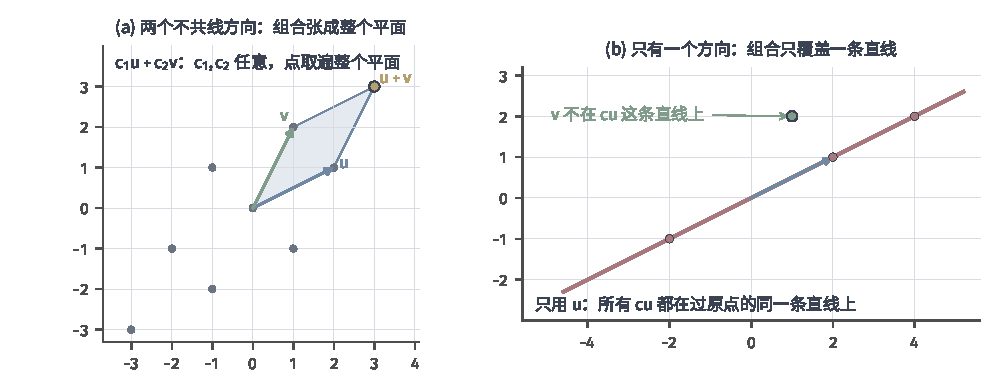
\includegraphics[width=169mm]{figures/01-mathematical-preliminaries-upper/02-linear-spaces/matplotlib/ls-linear-combination-span/ls-linear-combination-span.pdf}
  \caption{两个方向与一个方向的张成范围。左：$\bm u=(2,1)$（蓝箭头）与$\bm v=(1,2)$（绿箭头）的全部加权组合取遍整个平面，浅蓝平行四边形标出$0,\bm u,\bm u+\bm v,\bm v$，灰点为整数系数格点，黄点为$\bm u+\bm v=(3,3)$。右：只有$\bm u$一个方向时，组合$\{c\bm u\}$只是过原点的一条直线（红线），$\bm v$不在其上。两图坐标等比例，为解析教学例。}
  \label{fig:ls-linear-combination-span}
\end{figure*}

\paragraph{零向量的表示与线性无关}
表示是否冗余，要看零向量能否被非平凡地表示。若
\begin{equation}
 a_1\bm v_1+\cdots+a_k\bm v_k=\bm0
 \label{eq:linear-algebra-independence-relation}
\end{equation}
仅在全部$a_j=0$时成立，就称这组向量\term{线性无关}（linearly independent）；
否则称为\term{线性相关}（linearly dependent），即存在不全为零的系数使式
\eqref{eq:linear-algebra-independence-relation}成立。线性相关时挑出一个非零
系数$a_j$并移项，就能把$\bm v_j$写成其余向量的线性组合，说明这个方向重复了
已有方向能到达的范围。

在贯穿例\eqref{eq:linear-algebra-nearly-collinear-design}中，
$a_1\bm c_1+a_2\bm c_2=(a_1+a_2)\bm c_1+a_2\varepsilon\bm q$。
$\bm c_1$与$\bm q$线性无关，所以$\varepsilon\neq0$时两个系数只能都为零；
$\varepsilon=0$时却有$\bm c_1-\bm c_2=\bm0$。因此近共线和线性无关不同：
前者描述接近退化的程度，后者是精确的是非判断。

“能表示哪些对象”和“表示是否冗余”是两个独立的问题，分别由张成与线性无关回答。
在$\mathbb R^2$中取$\bm v_1=(1,0)^{\top}$、$\bm v_2=(0,1)^{\top}$，
$a_1\bm v_1+a_2\bm v_2=(a_1,a_2)^{\top}$可以取到平面上每个点，系数被目标点
唯一确定，这是“足够且无冗余”。只取$\bm v_1$一组方向，能到达的只是一条直线，
张成不够；再把$\bm v_3=(1,1)^{\top}$加入前两组，能到达的点仍只是整个平面，
$(1,1)^{\top}$却有$a_1=a_2=0,a_3=1$与$a_1=a_2=1,a_3=0$两组系数，这是
张成足够但表示冗余。图~\ref{fig:vol1-add-linear-redundant-directions}把这两种
表示画到同一个平面上。
\begin{figure}[!htb]
  \centering
  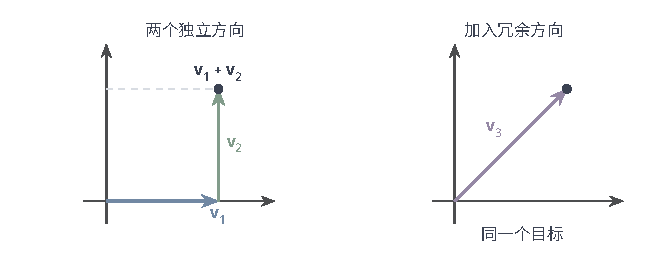
\includegraphics[width=112mm]{figures/01-mathematical-preliminaries-upper/02-linear-spaces/tikz/comprehension-additions/linear-redundant-directions.pdf}
  \caption{冗余方向与重复表示。取$\bm v_1=(1,0)^{\top}$、$\bm v_2=(0,1)^{\top}$与$\bm v_3=(1,1)^{\top}$。左图沿$\bm v_1$再沿$\bm v_2$，右图直接沿$\bm v_3$，到达同一个目标；前两向量已能表示平面中的每个向量，加入$\bm v_3$只使生成组冗余。两图坐标等比例。}
  \label{fig:vol1-add-linear-redundant-directions}
\end{figure}
存在性来自张成：张成之内的对象必有一组系数。唯一性来自线性无关：若同一对象
有两组系数，相减得到式\eqref{eq:linear-algebra-independence-relation}，
无关性保证两组系数完全相同。

反过来，唯一性也蕴含无关性。若存在一组不全为零的系数使线性组合为零，把这组
系数加到某个对象的一组表示上，就得到同一对象的第二组表示，表示不再唯一。
所以“张成内每个对象的系数唯一”与“零向量只有平凡表示”是同一件事的两面，
这正是后面坐标定义可以放心使用的根据。

\subsection{基与维数}
\label{sec:ls-basis-dimension}

\paragraph{基的抽取与扩充}
张成保证表示存在，无关保证表示唯一；同时做到这两条的一组向量，就是整个空间的
一把“尺子”。同时满足张成和线性无关的一组向量称为\term{基}（basis）：它足够
到达整个空间，又不重复。从任一有限生成组中反复抽取：若某成员能写成其余向量的
线性组合，删去它不会缩小张成范围，继续检查直到剩下的向量两两不可由其余表示，
最终得到一组线性无关的生成向量，即基。反过来，任一线性无关组可以逐次加入不在
其张成空间中的向量，直至扩充成基：每加入一个新方向，张成范围严格扩大；有限
空间迟早被填满，停止时留下的就是基。两条路线互补：抽取把冗余生成组压成基，
扩充把无关组补成基。

\paragraph{维数}
基的向量个数称为空间的\term{维数}（dimension）$\dim V$。这里有一个必须
先回答的问题：换一组基，个数会不会变？答案由交换引理给出。
\begin{theorem}[交换引理]
\label{thm:ls-exchange-lemma}
若$\bm u_1,\ldots,\bm u_r$线性无关，且每个$\bm u_i$都属于
$\operatorname{span}\{\bm v_1,\ldots,\bm v_s\}$，则$r\leq s$；并且这$r$个
$\bm u_i$可以逐个换入原生成组、换出同样多个$\bm v_j$，每次换完新组仍张成
原来的空间。
\begin{proof}
从生成组$G_0=\{\bm v_1,\ldots,\bm v_s\}$开始。因为$\bm u_1\in\operatorname{span}G_0$，
它可写成若干$\bm v_j$的组合；这些系数不能全为零，否则$\bm u_1=\bm0$，与
$\bm u_1,\ldots,\bm u_r$线性无关矛盾。取某个系数非零的$\bm v_j$，把它解出来：
$\bm v_j$可由$\bm u_1$与其余$\bm v$的组合表示，于是用$\bm u_1$换出$\bm v_j$，
新组$G_1$与$G_0$张成同一个空间。

一般地，第$i-1$步后的组$G_{i-1}$由$\bm u_1,\ldots,\bm u_{i-1}$和
$s-(i-1)$个幸存的$\bm v$组成，且与$G_0$张成同一空间。于是
$\bm u_i\in\operatorname{span}G_{i-1}$。若$\bm u_i$只用
$\bm u_1,\ldots,\bm u_{i-1}$就能表示，它与前面$i-1$个方向重复，违反
线性无关；所以表达式中至少一个幸存$\bm v$的系数非零，把它解出并换入
$\bm u_i$，张成范围不变。只要还有幸存$\bm v$，这一步就能做下去。

若$r>s$，换满$s$次以后组内只剩$\bm u_1,\ldots,\bm u_s$，却仍有
$\bm u_{s+1}$待入列；它属于$\operatorname{span}G_s=\operatorname{span}\{\bm u_1,\ldots,\bm u_s\}$，
与$r$个$\bm u$线性无关矛盾。故$r\leq s$，而上面的逐次交换正是定理要求的
换入换出过程。
\end{proof}
\end{theorem}

由此维数才是良定义的。任取两组基：把第一组看成无关组、第二组看成生成组，得
$r\leq s$；互换两组的角色又得$s\leq r$，所以$r=s$，换基不改变基的个数。
只含零向量的空间允许空基，维数为$0$。这一有限维结论支持后面的基扩充与维数
计算，不直接推广到无限维函数展开。$\mathbb R^d$的标准基
$\bm e_1,\ldots,\bm e_d$（第$j$个坐标为$1$、其余为$0$）是一组基，故
$\dim\mathbb R^d=d$；$P_k$的基为$1,t,\ldots,t^k$，故$\dim P_k=k+1$。

\section{子空间}
\label{sec:ls-subspaces}
\label{sec:linear-algebra-relations}
\label{sec:linear-algebra-subspace-relations}

固定同一个有限维实空间$V$，本节研究它的子空间怎样包含、相交与组合：包含比较
两个范围的大小，交找出公共方向，和合并两组方向，直和进一步要求分解唯一。这里
比较的始终是同一环境中的线性范围，不涉及长度或夹角。

\subsection{子空间包含}
\label{sec:ls-subspace-inclusion}

若子空间$U$的每个元素都属于子空间$W$，就记$U\subseteq W$。包含比较的是对象
范围：$U$的全部方向都在$W$中。取$U$的一组基，它在$W$中仍线性无关，按
~\ref{sec:ls-basis-dimension}节的基扩充补成$W$的基；只要$U$不占满$W$，
新增方向就不会是空的，因此$\dim U\leq\dim W$。

包含且同维，结论立刻收紧为相等。$\dim U=\dim W$时，$U$的基扩充成$W$的基
不需要新增任何方向，它本身已经张成$W$，故$U=W$。

反过来，同维本身推不出包含。平面中的两条不同直线维数都是$1$，却互不包含：
维数只数方向的个数，不管这些方向具体指向哪里。

把$U$的基扩充为$W$的基时，新增方向的个数恰为$\dim W-\dim U$，记录
$U$之外还有多少自由度。后面核与像、商空间的维数计算，都复用这一“先取已有基、
再补新方向”的做法。

\subsection{交空间}
\label{sec:ls-intersection}

两个子空间$U,W\subseteq V$的交$U\cap W$由同时属于二者的元素组成。它仍是
子空间：$\bm x,\bm y\in U\cap W$时二者既在$U$也在$W$，故$a\bm x+b\bm y$
同属两边。

交也是同时包含在$U$与$W$中的最大子空间：任何想同时装下两边公共方向的子空间，
装下的只能是交里的元素。平面中的画面帮着理解：两条重合的直线交出整条直线；
两条不同直线只交出零子空间。交为零只说明没有公共的非零方向，并不声称二者
合起来覆盖整个平面。

当$U,W$分别由齐次线性约束描述时，交就是同时满足两组约束的解集合。例如
$U=\{\bm x:x_1=0\}$与$W=\{\bm x:x_2=0\}$的交是
$\{\bm x:x_1=x_2=0\}$。集合与约束的对应在这里建立，具体消元求基留到求解章。

\subsection{和空间}
\label{sec:ls-sum}

\paragraph{维数公式}
两组方向联合能到达的对象组成和空间
$U+W=\{\bm u+\bm w:\bm u\in U,\ \bm w\in W\}$。它对线性组合封闭，是同时
包含$U,W$的最小子空间。注意并集$U\cup W$一般不对相加封闭，和空间补入了必要的
线性组合。

先取$U\cap W$的一组基，分别扩充为$U$与$W$的基；两组新增方向与共有基合起来
张成$U+W$。若其线性组合为零，把$U$一侧移到$W$一侧便得到交中的向量，各自
扩充基的无关性迫使新增系数为零，共有系数也为零。因此
\begin{equation}
 \dim(U+W)=\dim U+\dim W-\dim(U\cap W).
 \label{eq:ls-dimension-formula}
\end{equation}
被减去的维数正是两边重复计入的公共方向，而不是两个集合元素个数的差。例如在
$\mathbb R^3$中$U=\operatorname{span}\{\bm e_1,\bm e_2\}$、
$W=\operatorname{span}\{\bm e_2,\bm e_3\}$，交为$\operatorname{span}\{\bm e_2\}$，
$\dim(U+W)=3=2+2-1$；若把两条不同坐标轴当作$U,W$，交为零，和的维数直接相加。

\subsection{直和}
\label{sec:ls-direct-sum}

\paragraph{补空间}
平面上一条直线只能记录部分方向；再取一条不平行的直线，平面中的每个向量就能
拆成两个部分，各占一条直线上的一份。把这种“分解唯一”的要求写成代数条件：
若$U\cap W=\{\bm0\}$，则$U+W$中每个向量的两部分分解唯一：若
$\bm u_1+\bm w_1=\bm u_2+\bm w_2$，移项得$\bm u_1-\bm u_2=\bm w_2-\bm w_1$，
左边在$U$、右边在$W$，故同属交，只能是零，于是$\bm u_1=\bm u_2$、
$\bm w_1=\bm w_2$。这时称和为\term{直和}（direct sum），记为$U\oplus W$。
唯一分解不要求正交：平面中的两条非平行直线就构成直和，实际写出分量还要选择
相应基。

要写$V=U\oplus W$，还须满足$U+W=V$，这样的$W$称为$U$在$V$中的
\term{补空间}（complement）。
有限维中由基扩充总能选出这样的$W$，但选择一般不唯一：在平面中给一条直线选补空间，
任何不平行于它的直线都可以。指定内积以后的正交补是另一回事，由内积一节介绍，
不能把一般补空间自动称为正交补。

\section{坐标与换基}
\label{sec:ls-coordinates-change-of-basis}
\label{sec:linear-algebra-coordinate-conversions}

基保证表示唯一以后，本节研究怎样从基读出坐标，以及换一组基时同一对象的记录怎样
转换。被动换基只改变记录方式，不是对对象施加新的作用。

\subsection{坐标}
\label{sec:ls-coordinates}
\label{sec:linear-algebra-coordinates}

固定有序基$\mathcal B=(\bm b_1,\ldots,\bm b_d)$后，对象$\bm v$唯一写成
$\sum_{j=1}^d x_j\bm b_j$。系数列
$[\bm v]_{\mathcal B}=(x_1,\ldots,x_d)^{\top}$称为$\bm v$在基$\mathcal B$
下的\term{坐标}（coordinates）。存在性来自张成，唯一性来自线性无关，所以坐标
映射$\bm v\mapsto[\bm v]_{\mathcal B}$是线性双射。如图~\ref{fig:ls-basis-coordinates}
所示，同一个几何向量在标准基下读出$(1,2)$，在斜基$\bm b_1=(2,1)$、
$\bm b_2=(-1,1)$下读出$(1,1)$：向量本身没有移动，只是沿不同的基尺子去量。
\begin{figure*}[htbp]
  \centering
  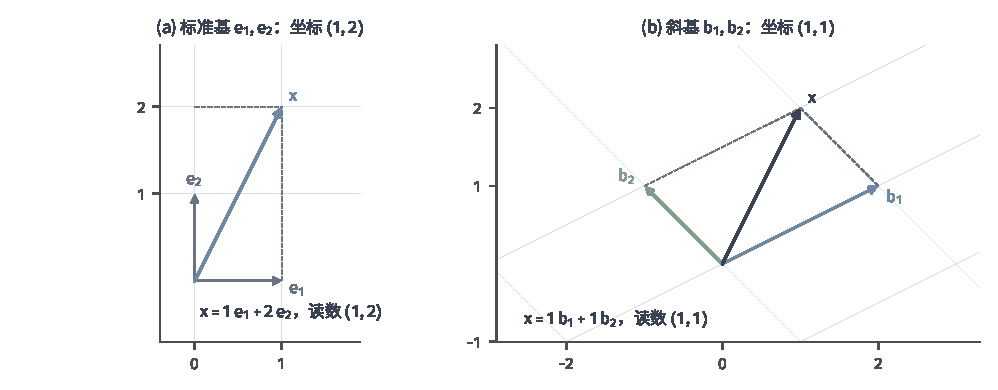
\includegraphics[width=169mm]{figures/01-mathematical-preliminaries-upper/02-linear-spaces/matplotlib/ls-basis-coordinates/ls-basis-coordinates.pdf}
  \caption{同一向量在两组基下的坐标。左：标准基$\bm e_1,\bm e_2$（灰箭头）下，向量$\bm x=(1,2)$（蓝箭头）的坐标为$(1,2)$，虚线为向坐标轴的垂线。右：斜基$\bm b_1=(2,1)$（蓝）、$\bm b_2=(-1,1)$（绿）下，同一个$\bm x$满足$\bm x=\bm b_1+\bm b_2$，坐标为$(1,1)$，浅色斜线为斜基网格，虚线为平行四边形读法。两图坐标系相同。}
  \label{fig:ls-basis-coordinates}
\end{figure*}

基的顺序同时固定：交换$\bm b_1,\bm b_2$，对象不变，坐标列的前两个数也交换。
在$\mathbb R^d$中直接写数字列，通常是默认使用标准基$\bm e_1,\ldots,\bm e_d$。
函数基展开完全如此：函数是对象，展开系数是坐标，例如$f_{a,b}=a\cdot1+b\cdot t$
在基$(1,t)$下的坐标是$(a,b)^{\top}$。坐标个数是维数，不能由某个冗余记录的
长度直接推断。

对象不变时，坐标仍可能很不一样。固定$\delta=0.1$并令
\begin{equation}
 \bm y=\bm c_1+\delta\bm q=\begin{bmatrix}1\\1.1\\0.9\end{bmatrix}.
 \label{eq:linear-algebra-nearly-collinear-target}
\end{equation}
在$\mathcal B_0=(\bm c_1,\bm q)$下坐标是$(1,\delta)^{\top}$。若
$\varepsilon\neq0$，改用同一平面上的基$\mathcal B_\varepsilon=(\bm c_1,\bm c_2)$，
则
\begin{equation}
 \bm y=\left(1-\frac{\delta}{\varepsilon}\right)\bm c_1
       +\frac{\delta}{\varepsilon}\bm c_2.
 \label{eq:linear-algebra-coordinate-instability}
\end{equation}
$\varepsilon=0.01$时坐标成为$(-9,10)^{\top}$，但$\bm y$没有改变。两个很大的
系数在几乎同向的基向量上相消，不能据此判断原对象很大；这种系数对基接近退化的
敏感，将在误差分析章定量讨论。

\subsection{换基}
\label{sec:ls-change-basis}

设$\mathcal C$是另一组基。把各$\bm b_j$的$\mathcal C$坐标排成列，得到换基矩阵
$\bm S_{\mathcal C\leftarrow\mathcal B}$；保持线性组合给出
\begin{equation}
 [\bm v]_{\mathcal C}
 =\bm S_{\mathcal C\leftarrow\mathcal B}[\bm v]_{\mathcal B}.
 \label{eq:linear-algebra-coordinate-change}
\end{equation}
沿反方向换基能恢复原坐标，两个坐标变换互逆。在贯穿例中，
$\bm S_{\mathcal B_0\leftarrow\mathcal B_\varepsilon}
=\begin{bmatrix}1&1\\0&\varepsilon\end{bmatrix}$，反向求坐标要除以
$\varepsilon$，已提示小扰动可能被放大。此处改变的是记录方式，不是对对象施加
新的物理变换。图~\ref{fig:vol1-add-linear-change-basis}核对了这种区别：目标
位置没有移动，改变的只是沿哪两条基方向累加，以及每条方向取多少份。
\begin{figure}[!htb]
  \centering
  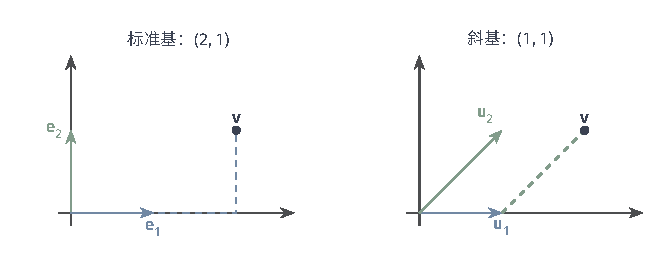
\includegraphics[width=112mm]{figures/01-mathematical-preliminaries-upper/02-linear-spaces/tikz/comprehension-additions/linear-change-basis.pdf}
  \caption{同一向量的两套坐标。左图使用标准基，$\bm v=(2,1)^{\top}$的坐标为$(2,1)^{\top}$；右图使用$\bm c_1=(1,0)^{\top}$、$\bm c_2=(1,1)^{\top}$，同一$\bm v$的坐标为$(1,1)^{\top}$。虚线表示相应的向量相加，两图的环境坐标比例相同。}
  \label{fig:vol1-add-linear-change-basis}
\end{figure}

若再换到第三组基$\mathcal D$，中间坐标应相消：
$\bm S_{\mathcal D\leftarrow\mathcal B}
=\bm S_{\mathcal D\leftarrow\mathcal C}\bm S_{\mathcal C\leftarrow\mathcal B}$。
这是逐坐标代入的结果：先按$\mathcal B$读出$\bm v$，再用$\mathcal C$坐标表示，
最后换到$\mathcal D$，中间那套坐标不留下痕迹。

被动换基与主动作用必须分开。换基时对象不动、记录改变，式
\eqref{eq:linear-algebra-coordinate-change}两侧是同一个$\bm v$的两套坐标；
主动作用则是固定坐标把对象送到另一个对象，例如把向量旋转或缩放。图
~\ref{fig:ls-passive-change-vs-active-map}把两种情形并排放置：左图中向量位置
不动，读数从$(3,3)$变成$(2,1)$；右图中坐标系不动，向量$\bm x=(3,3)$被切变
$\bm A=\begin{bmatrix}1&1\\0&1\end{bmatrix}$搬到$\bm A\bm x=(6,3)$。两者
乘法形式相似，含义不同，不能把所有乘矩阵都理解成换基；主动作用在
~\ref{sec:ls-linear-maps}节作为线性映射建立。
\begin{figure*}[htbp]
  \centering
  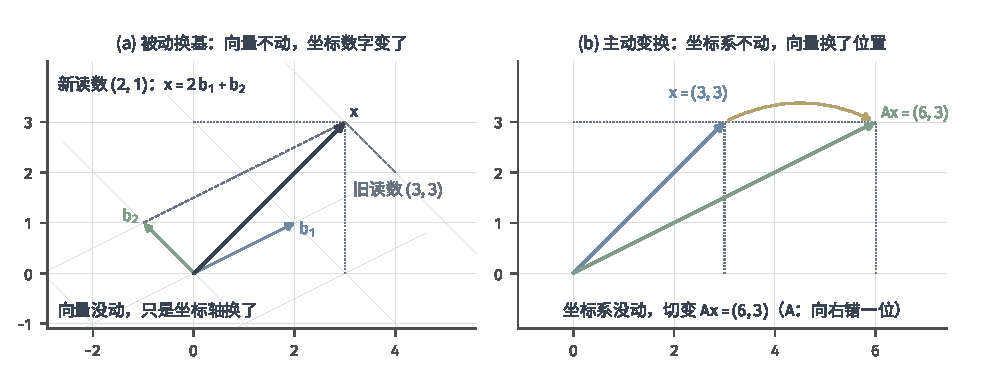
\includegraphics[width=169mm]{figures/01-mathematical-preliminaries-upper/02-linear-spaces/matplotlib/ls-passive-change-vs-active-map/ls-passive-change-vs-active-map.pdf}
  \caption{被动换基与主动变换的对照，两图使用同一个初始向量$\bm x=(3,3)$。左（被动换基）：箭头位置不动（深色），旧标准读数用点线投影读出$(3,3)$；新斜基$\bm b_1=(2,1)$（蓝）、$\bm b_2=(-1,1)$（绿）与浅色斜网格下，$\bm x=2\bm b_1+\bm b_2$，新读数为$(2,1)$。右（主动变换）：标准坐标系不动，$\bm x$（蓝）被切变映到$\bm A\bm x=(6,3)$（绿），黄色弧线表示搬动过程。}
  \label{fig:ls-passive-change-vs-active-map}
\end{figure*}

\section{线性映射}
\label{sec:ls-linear-maps}
\label{sec:linear-algebra-matrices-linear-maps}

对象之间的作用怎样决定输出、又保留或丢失了哪些输入信息，是本节的问题。选定输入与
输出两端的基以后，作用被记录为矩阵；核、像与秩零度定理描述被消去和被保留的
自由度，并据此判断何时可以由输出反求输入。

\subsection{线性映射}
\label{sec:ls-linear-map-definition}
\label{sec:linear-algebra-maps}

保持线性组合的作用称为\term{线性映射}（linear map）$T:V\to W$：
\begin{equation}
 T(a\bm x+b\bm y)=aT\bm x+bT\bm y,
 \qquad \bm x,\bm y\in V,\ a,b\in\mathbb R.
 \label{eq:ls-linear-map-def}
\end{equation}
特别有$T\bm0=\bm0$。第~\ref{chap:sets-functions-and-proofs}章
~\ref{sec:prelim-linear-actions-composition}节已经看到
矩阵乘向量满足这条规则，这里把它作为作用的一般定义。

给定输入基$\mathcal B=(\bm b_1,\ldots,\bm b_d)$和输出基$\mathcal C$，只要
记录每个基向量的像就能记录整个映射：由线性性，$T(\sum_j x_j\bm b_j)
=\sum_j x_jT\bm b_j$。把$[T\bm b_j]_{\mathcal C}$作为第$j$列，得到矩阵
$\bm A=[T]_{\mathcal C\leftarrow\mathcal B}\in\mathbb R^{m\times d}$，并有
\begin{equation}
 [T\bm v]_{\mathcal C}
 =[T]_{\mathcal C\leftarrow\mathcal B}[\bm v]_{\mathcal B}
 =\bm A[\bm v]_{\mathcal B}.
 \label{eq:linear-algebra-map-matrix-representation}
\end{equation}
列数是输入维数，行数是输出维数。图~\ref{fig:ch06-object-coordinate-map}中两条
路径给同一结果，表明矩阵是映射在两端坐标下的表示，不是映射本身的全部含义：改变
两端任一组基通常改变数表，却仍记录同一个映射。
\begin{figure}[htbp]
  \centering
  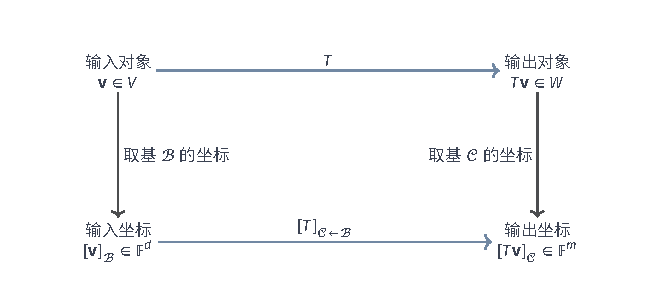
\includegraphics[width=112.0mm]{figures/01-mathematical-preliminaries-upper/02-linear-spaces/tikz/ch06-object-coordinate-map/figure.pdf}
  \caption{先作用于对象再取坐标，与先取输入坐标再乘矩阵，得到相同输出坐标。横向箭头改变对象或数值，竖向箭头只改变记录方式。}
  \label{fig:ch06-object-coordinate-map}
\end{figure}

设计矩阵$\bm X_\varepsilon$表示$T_\varepsilon:\mathbb R^2\to\mathbb R^3$，
$\bm w\mapsto w_1\bm c_1+w_2\bm c_2$。输入是两个系数，输出是三个样本的拟合值，
二者不能当成同一个空间中的向量。

带常数偏置的规则$\bm x\mapsto\bm A\bm x+\bm b$在$\bm b\neq\bm0$时为
\term{仿射映射}（affine map），不是线性映射：它把$\bm0$送到$\bm b$，而线性
映射必将$\bm0$送到$\bm0$。增广坐标
\begin{equation*}
 \begin{bmatrix}\bm A&\bm b\\\bm0^{\top}&1\end{bmatrix}
 \begin{bmatrix}\bm x\\1\end{bmatrix}
 =\begin{bmatrix}\bm A\bm x+\bm b\\1\end{bmatrix}
\end{equation*}
对增广空间是线性的，但原输入被限制在末坐标为$1$的仿射集合上，不能因此声称原映射
线性。仿射解集的几何在求解章直接使用这一形式。

\subsection{核与像}
\label{sec:ls-kernel-image}

被送到零的输入集合称为\term{零空间}（核，kernel）：
$\ker T=\{\bm x\in V:T\bm x=\bm0\}$；所有可到达的输出集合称为\term{像空间}
（像，image）：$\operatorname{im}T=\{T\bm x:\bm x\in V\}$。二者都是子空间：
若$T\bm x=T\bm y=\bm0$，则$T(a\bm x+b\bm y)=\bm0$；若$\bm u=T\bm x$、
$\bm v=T\bm y$，则$a\bm u+b\bm v=T(a\bm x+b\bm y)$。核记录被映射完全消去的
独立输入方向，像记录可达的输出范围；二者分别位于输入端与输出端，不能当作同一空间
中的两个集合直接比较。

例如用三个响应读取四个分量，教学矩阵$\bm S=[\,\bm I_3\mid\bm1\,]$满足
$\bm S(1,1,1,1)^{\top}=\bm S(0,0,0,2)^{\top}=(2,2,2)^{\top}$。两输入之差
$(1,1,1,-1)^{\top}$在核中，所以仅凭响应无法区分它们。这演示的是线性不可辨识性：
两个输入相差核方向时输出相同，具体约束下的合法输入范围另有限制。

\subsection{秩与零度}
\label{sec:ls-rank-nullity}

\paragraph{秩零度定理与独立约束}
像的维数称为\term{秩}（rank）$\operatorname{rank}T=\dim\operatorname{im}T$，
核的维数称为\term{零度}（nullity）$\dim\ker T$。
\begin{theorem}[秩零度定理]
\label{thm:ls-rank-nullity}
\label{thm:linear-algebra-rank-nullity}
有限维线性映射$T:V\to W$满足
\begin{equation}
 \dim V=\dim\ker T+\dim\operatorname{im}T,
 \qquad\text{即}\qquad
 \dim V=\dim\ker T+\operatorname{rank}T.
 \label{eq:ls-rank-nullity}
\end{equation}
\end{theorem}
\begin{proof}
取核的一组基$\bm v_1,\ldots,\bm v_r$并扩充成$V$的基
$\bm v_1,\ldots,\bm v_d$。前$r$个基向量的像为零，所以其余像
$T\bm v_{r+1},\ldots,T\bm v_d$张成像。若$\sum_{j>r}a_jT\bm v_j=\bm0$，
则$\sum_{j>r}a_j\bm v_j$属于核，能由前$r$个基向量表示；整个基的线性无关性
迫使全部$a_j=0$，所以这些像也是无关组。像的维数为$d-r$，结论成立。
\end{proof}
对矩阵$\bm A\in\mathbb R^{m\times d}$，记$\operatorname{rank}\bm A$为其映射
的秩，有$d=\dim\ker\bm A+\operatorname{rank}\bm A$。秩计数独立的输出方向，
零度计数被消去的独立输入方向，二者此消彼长。图
~\ref{fig:ls-kernel-image-rank-nullity}给出两个几何化算例：被映到零的方向与
实际用到的输出方向，维数相加恰为定义域维数。
\begin{figure*}[htbp]
  \centering
  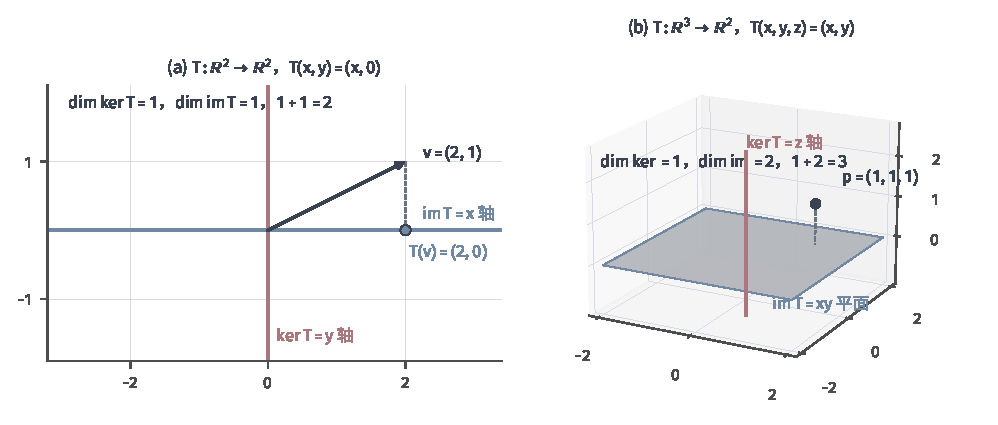
\includegraphics[width=169mm]{figures/01-mathematical-preliminaries-upper/02-linear-spaces/matplotlib/ls-kernel-image-rank-nullity/ls-kernel-image-rank-nullity.pdf}
  \caption{核与像的维数此消彼长。左：$T(x,y)=(x,0)$把平面映到$x$轴，核是$y$轴（红直线）、像是$x$轴（蓝直线），$\dim\ker T=1$、$\dim\operatorname{im}T=1$，$1+1=2$；样本$\bm v=(2,1)$被映到$(2,0)$。右：$T(x,y,z)=(x,y)$把三维空间映到$xy$平面，核是$z$轴（红直线）、像是整个$xy$平面（浅蓝），$\dim\ker T=1$、$\dim\operatorname{im}T=2$，$1+2=3$。两图为解析教学例。}
  \label{fig:ls-kernel-image-rank-nullity}
\end{figure*}

对$\bm A\in\mathbb R^{m\times d}$，$\operatorname{rank}\bm A\leq\min(m,d)$。
$\operatorname{rank}\bm A=d$称为满列秩，输入方向全部被保留；
$\operatorname{rank}\bm A=m$称为满行秩，输出全部可达；二者统称
\term{满秩}（full rank）。形状不同时二者不能
同时成立：$m<d$时满行秩仍可能有非零核，$m>d$时满列秩仍可能有输出缺失。
这里以列张成空间读取秩；行秩等于列秩的证明在~\ref{sec:ls-dual-map}节由对偶
映射补齐。

\subsection{单射、满射与可逆性}
\label{sec:ls-injective-surjective-invertible}
\label{sec:prelim-inverse-matrices}

\paragraph{逆与单侧逆}
第~\ref{chap:sets-functions-and-proofs}章~\ref{sec:prelim-function-types}节按一般
函数定义过单射、满射与双射。对线性
映射，单射等价于核为零：$T\bm x=T\bm y$当且仅当$\bm x-\bm y\in\ker T$，
核为零时输出相同必输入相同。满射等价于像等于整个输出空间。二者同时成立时得到
线性双射，每个输出恰有一个原输入，逆映射$T^{-1}:W\to V$也是线性的。有限维且
输入输出维数相等时，秩零度定理给出单射、满射、双射等价；维数不同则须分别判断，
不把矩形矩阵的满秩直接说成双侧可逆。

对$n$阶方阵$\bm A$，若存在$n$阶方阵$\bm B$满足
$\bm A\bm B=\bm B\bm A=\bm I_n$，就称$\bm A$可逆，$\bm B$为
\term{逆矩阵}（inverse matrix），记作$\bm A^{-1}$。两边的单位矩阵条件分别
保证先后两个方向的乘法都能撤销。若$\bm B,\bm C$都满足条件，则
\[
 \bm B=\bm B\bm I_n=\bm B(\bm A\bm C)
 =(\bm B\bm A)\bm C=\bm I_n\bm C=\bm C,
\]
所以逆矩阵唯一，每次改写只使用结合律，没有交换矩阵次序。

可逆要回答的问题是：给一个输出，能否唯一还原输入。先看最容易还原的情形——
对角矩阵把各坐标分别乘以一个数，坐标之间互不影响，撤销它就是逐坐标除以这些
数。每个$d_i\neq0$时，
$\operatorname{diag}(d_1,\ldots,d_n)^{-1}
=\operatorname{diag}(1/d_1,\ldots,1/d_n)$，例如
$\operatorname{diag}(2,1)$的逆为$\operatorname{diag}(1/2,1)$。

这一简单情形同时划出不可逆的边界：若某个$d_i=0$，相应坐标被压为零，两个只在
该坐标不同的输入给出相同输出，反求必然失败。对角情形把“可逆等于每个输入方向
都能被原样读回”看得最清楚；一般矩阵把坐标掺在一起，不能逐坐标处理，但撤销
的目标相同：对一般可逆矩阵，$\bm A\bm x=\bm y$左乘$\bm A^{-1}$，得到唯一的
$\bm x=\bm A^{-1}\bm y$。

两个可逆方阵接连作用时，撤销过程应当倒过来执行，这与逆映射的复合规则相同：
若$\bm A,\bm B$都是$n$阶可逆方阵，则
\begin{equation}
 (\bm A\bm B)^{-1}=\bm B^{-1}\bm A^{-1}.
 \label{eq:ls-inverse-product}
\end{equation}
验证：$(\bm A\bm B)(\bm B^{-1}\bm A^{-1})
=\bm A(\bm B\bm B^{-1})\bm A^{-1}=\bm I_n$，反方向也等于单位矩阵。这里的
逆一般不是逐元素取倒数；矩阵乘法的行列混合决定了它必须作为整体计算。

矩形矩阵没有方阵意义的双侧逆。满列秩的长矩阵可有左逆$\bm L$使
$\bm L\bm A=\bm I_d$，满行秩的宽矩阵可有右逆$\bm R$使$\bm A\bm R=\bm I_m$，
但这些单侧逆一般不唯一。此处只判断恢复关系是否存在；如何通过分解应用逆、多解时
如何选择代表，分别由运算章与求解章回答。

\section{对偶空间}
\label{sec:ls-dual-spaces}

怎样把一个对象线性地读成一个数，读取规则又怎样随映射改变？本节从线性泛函构造对偶
基，再由复合定义对偶映射并给出转置表示；这一代数构造不依赖长度、夹角或内积，
内积意义下的伴随在运算章建立。

\subsection{对偶空间}
\label{sec:ls-dual-space}

读取多项式在$t=0$处的取值、取信号的第一个样本、计算一组系数加权和，都是把一个
对象读成一个数。保持线性组合的标量读取称为\term{线性泛函}（linear functional）：
$\varphi:V\to\mathbb R$满足$\varphi(a\bm x+b\bm y)
=a\varphi(\bm x)+b\varphi(\bm y)$。读取一个坐标、计算一个线性加权和都是
线性泛函；同一个对象可以接受多种读取。全部线性泛函按逐点加法与数乘
$(\alpha\varphi+\beta\psi)(\bm x)=\alpha\varphi(\bm x)+\beta\psi(\bm x)$
组成线性空间，称为$V$的\term{对偶空间}（dual space）$V^*$。输入向量是被读取
的对象，泛函是读取规则，二者属于不同类型。

\paragraph{对偶基}
对$V$的基$\mathcal B=(\bm b_1,\ldots,\bm b_d)$，逐个定义泛函
$\varphi_j\in V^*$使
\begin{equation}
 \varphi_j(\bm b_i)=\delta_{ji}
 =\begin{cases}1,&i=j,\\0,&i\neq j.\end{cases}
 \label{eq:ls-dual-basis-def}
\end{equation}
任意$\varphi\in V^*$都能唯一展开为$\varphi=\sum_j\varphi(\bm b_j)\varphi_j$：
两边在$\bm b_i$上取值即得系数，无关性由$\varphi_j$的取值约束保证。这组
$\varphi_1,\ldots,\varphi_d$称为$\mathcal B$的\term{对偶基}（dual basis），
因而$\dim V^*=d=\dim V$。坐标可逐项恢复：$x_j=\varphi_j(\bm v)$。
标准基$\bm e_j$的对偶基就是第$j$坐标投影$x_j$。换一组基，对偶基随之更换：
取$\bm b_1=(1,1)^{\top}$、$\bm b_2=(1,0)^{\top}$，解$\varphi_j(\bm b_i)=\delta_{ji}$
得$\varphi_1(x,y)=y$、$\varphi_2(x,y)=x-y$；读取规则随基改变，但$\dim V^*$
不变。图~\ref{fig:ls-dual-basis-readout}在平面中把这种逐项读取画出来：对偶
方向$\bm b^1,\bm b^2$分别只在一个基方向上读到$1$，其余读到$0$。
\begin{figure}[htbp]
  \centering
  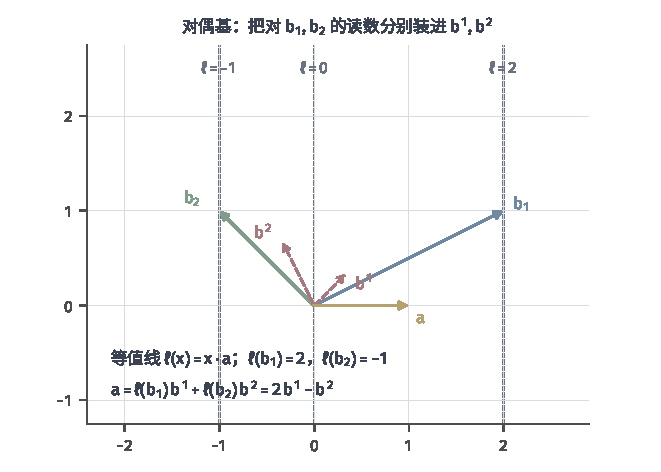
\includegraphics[width=112mm]{figures/01-mathematical-preliminaries-upper/02-linear-spaces/matplotlib/ls-dual-basis-readout/ls-dual-basis-readout.pdf}
  \caption{对偶读取的几何示意。蓝箭头$\bm b_1=(2,1)$、绿箭头$\bm b_2=(-1,1)$为基向量；红色虚线箭头为满足$\varphi_i(\bm b_j)=\delta_{ij}$的对偶基方向$\bm b^1=(1/3,1/3)$、$\bm b^2=(-1/3,2/3)$（本章中对偶基是读取规则；画成平面箭头借用的是内积意义下的对应向量，该对应在运算章建立）。黄色箭头$\bm a=(1,0)$给出读取$\ell(\bm x)=\bm a\cdot\bm x$，灰色虚线为等值线$\ell=c$（$c=-1,0,2$）；$\ell(\bm b_1)=2$、$\ell(\bm b_2)=-1$，且$\bm a=2\bm b^1-\bm b^2$。}
  \label{fig:ls-dual-basis-readout}
\end{figure}

\subsection{对偶映射}
\label{sec:ls-dual-map}

已知$T:V\to W$和输出端的读取$f\in W^*$，输入$\bm x$经过$T$后被读成
$f(T\bm x)$。由这项复合定义\term{对偶映射}（dual map）$T':W^*\to V^*$，
\begin{equation}
 T'f=f\circ T,\qquad (T'f)(\bm x)=f(T\bm x),
 \label{eq:ls-dual-map-def}
\end{equation}
反向传递的是读取规则，并非对$T$求逆。$T'$保持线性组合。

设输入基$\mathcal B=(\bm b_1,\ldots,\bm b_d)$、输出基
$\mathcal C=(\bm c_1,\ldots,\bm c_m)$下$T$的矩阵为$\bm A$，即
$T\bm b_j=\sum_i a_{i,j}\bm c_i$，对应的对偶基分别为$\varphi_j^V$、
$\varphi_i^W$。取输出读取$f=\sum_i y_i\varphi_i^W$，则
\begin{equation*}
 (T'f)(\bm b_j)=f(T\bm b_j)
 =\sum_i y_i\varphi_i^W\left(\sum_k a_{k,j}\bm c_k\right)
 =\sum_i a_{i,j}y_i=(\bm A^{\top}\bm y)_j.
\end{equation*}
所以$T'f$在输入对偶基下的系数列为$\bm A^{\top}\bm y$，即对偶映射的矩阵是
\term{转置}（transpose）$\bm A^{\top}$。这一推导只使用线性性和坐标，不需要
长度、夹角或内积；内积把读取方向识别为某个向量的表示，由运算章另行建立。

$\ker T'$由在$\operatorname{im}T$上恒为零的读取组成。设$r=\operatorname{rank}T$，
在$\operatorname{im}T$上取基并扩充为$W$的基，相应对偶读取中只有$m-r$个在
$\operatorname{im}T$上为零，故$\dim\ker T'=m-r$。对$T'$应用秩零度定理，
$\operatorname{rank}T'=m-(m-r)=r=\operatorname{rank}T$。在矩阵记录下
$\operatorname{rank}(\bm A^{\top})=\operatorname{rank}\bm A$，即行秩等于
列秩，闭合了~\ref{sec:ls-rank-nullity}节留下的判据。

\section{商空间}
\label{sec:ls-quotient-spaces}

当相差某个子空间内方向的对象应视为同一结果时，怎样表示忽略差别以后剩余的信息？
本节以差属于子空间定义等价，验证类上的运算与代表元无关，由基扩充求维数，最后把
商空间与映射的像对应起来。

\subsection{等价类}
\label{sec:ls-equivalence-classes}
\label{sec:linear-algebra-equivalence-relations}

例如只读取仿射函数在$t=0$处的截距时，斜率不同的两个函数应当被视为同一结果：
它们在截距上没有区别。把这种“忽略指定方向”的直觉写成代数关系。设$U$是$V$的
子空间，规定$\bm x\sim\bm y$当且仅当$\bm x-\bm y\in U$。这是
第~\ref{chap:sets-functions-and-proofs}章~\ref{def:prelim-equivalence-relation}定义的
等价关系：$\bm x-\bm x=\bm0\in U$
给出自反性；$\bm x-\bm y\in U$蕴含$\bm y-\bm x\in U$给出对称性；
$(\bm x-\bm y)+(\bm y-\bm z)=\bm x-\bm z\in U$给出传递性。
$\bm x$的\term{等价类}（equivalence class）为
$\bm x+U=\{\bm x+\bm n:\bm n\in U\}$；两个类相等不要求当前选取的代表元相等，
只要求代表元之差落在$U$中。全部等价类把$V$划分成互不重叠的块。图
~\ref{fig:ls-quotient-equivalence-classes}把这一划分画出来：子空间$U$是
$x$轴，平面被一族平行于$U$的直线切成一条条等价类，同一条线上的任意两点之差
都落在$U$中。
\begin{figure}[htbp]
  \centering
  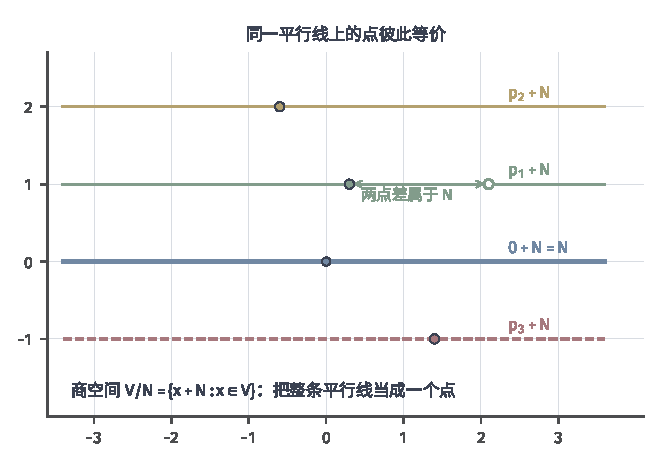
\includegraphics[width=112mm]{figures/01-mathematical-preliminaries-upper/02-linear-spaces/matplotlib/ls-quotient-equivalence-classes/ls-quotient-equivalence-classes.pdf}
  \caption{商空间的等价类。$V=\mathbb R^2$，子空间$U$为$x$轴（蓝线$0+U$）；每条平行直线$p+U=\{(x,p_y)\}$是一个等价类，图中画出$y=1$（绿）、$y=2$（黄）、$y=-1$（红虚线）。绿线上实点$(0.3,1)$与空心点$(2.1,1)$之差$(1.8,0)\in U$，故属同一类；商空间$V/U$把每条平行线当成一个点。}
  \label{fig:ls-quotient-equivalence-classes}
\end{figure}

\subsection{商空间}
\label{sec:ls-quotient-space}
\label{def:linear-algebra-quotient-space}

\paragraph{代表元无关}
全部等价类组成的集合$V/U$称为\term{商空间}（quotient space），其运算规定为
\begin{equation}
 (\bm x+U)+(\bm y+U)=(\bm x+\bm y)+U,
 \qquad
 a(\bm x+U)=a\bm x+U.
 \label{eq:ls-quotient-operations}
\end{equation}
换代表元$\bm x'=\bm x+\bm n_1$、$\bm y'=\bm y+\bm n_2$时，结果只相差
$\bm n_1+\bm n_2$或$a\bm n_1$，仍属于$U$，所以运算不依赖代表元。零类是
$U$本身，逆元为$-\bm x+U$，其余公理由$V$继承，$V/U$构成实线性空间。任务也
可以主动忽略一个指定子空间，不必先由误差尺度产生它；原对象、被忽略的方向和等价类
须分别记录。

取$U$的一组基$\bm u_1,\ldots,\bm u_s$并扩充为$V$的基
$\bm u_1,\ldots,\bm u_s,\bm v_1,\ldots,\bm v_t$。新增$\bm v_j$的等价类张成
$V/U$：任一$\bm x$写成两组基的组合，$U$部分落进零类被消去；这些类线性无关：
若$\sum_j a_j(\bm v_j+U)=U$，则$\sum_j a_j\bm v_j\in U$，它能由$\bm u_i$
表示，整个基的无关性迫使$a_j=0$。故商基有$t$个成员，
\begin{equation}
 \dim(V/U)=\dim V-\dim U.
 \label{eq:ls-quotient-dimension}
\end{equation}
例如仿射函数中只读取$t=0$处的截距时，零方向是$\operatorname{span}\{t\}$，
商空间只保留截距，被消去的是全部斜率方向。

\subsection{商映射}
\label{sec:ls-quotient-map}

自然映射$q:V\to V/U$把对象送到其等价类，$q(\bm x)=\bm x+U$。它线性：
$q(a\bm x+b\bm y)=(a\bm x+b\bm y)+U=a(\bm x+U)+b(\bm y+U)$，正是类上定义的
加法与数乘。它满射：$V/U$的每个类$\bm x+U$都有原代表$\bm x$。它的核恰为
$U$：$q(\bm x)=U$（零类）当且仅当$\bm x\in U$，即恰好被消去的方向组成这个
子空间。例如消去$\operatorname{span}\{t\}$后，截距类由$q(f_{a,b})=a+U$送出，
斜率$b$不在类中出现。

对$T:V\to W$取$U=\ker T$。规则$[\bm x]\mapsto T\bm x$不依赖代表元：
若$\bm x'=\bm x+\bm n$且$\bm n\in\ker T$，则$T\bm x'=T\bm x$。它线性、
满射到$\operatorname{im}T$，且核为零，因而是线性双射：
\begin{equation}
 V/\ker T\ \cong\ \operatorname{im}T.
 \label{eq:ls-first-isomorphism}
\end{equation}
压去全部丢失方向后，每个等价类恰对应一个可达输出；原映射本身未必具有双侧逆，
这里建立的是商空间与像之间的一一对应。

\section{矩阵表示的等价关系}
\label{sec:ls-matrix-equivalences}

不同矩阵是否记录同一个映射或同一个双线性读取？换基只改变记录、不改变对象，于是
同一对象在不同坐标下得到不同数表。本节分别在相似、相抵、合同内部讲清各自的坐标
约定、保持的不变量和验证条件，三者对象不同，不能混用。统一采用旧坐标
$\bm x=\bm P\bm x'$、$\bm y=\bm Q\bm y'$，带撇的是新坐标。本章只使用秩与
核维数等已经建立的量；迹、行列式的不变量在运算章相应定义后再补充，完整的实分裂
相似分类后置。

\subsection{相似}
\label{sec:ls-similarity}

\subsubsection{定义与含义}
\label{sec:ls-similarity-meaning}

同一个旋转，换一套坐标系以后写出来的数表并不相同；那么什么时候两个数表记录的是
同一个作用？固定同一个实线性自映射$T:V\to V$，比较它在两组基下的矩阵记录。
设旧基$\mathcal B$下坐标为$\bm x$，新基$\mathcal B'$下坐标为$\bm x'$，
旧矩阵$\bm A$满足$\bm y=\bm A\bm x$，新矩阵$\bm B$满足$\bm y'=\bm B\bm x'$。

旧坐标与新坐标由可逆换基矩阵联系：新基向量$\bm b_j'$在旧基下的坐标列拼成
$\bm P$的第$j$列，故对象的旧坐标$\bm x=\bm P\bm x'$，新坐标是旧坐标经
$\bm P$反向读出。$\bm P$可逆，因为两组基都能唯一表示$V$中的对象；反向
换基矩阵为$\bm P^{-1}$，把旧坐标换回新坐标。这里输入与输出是同一个空间、
同一组新基，所以输出坐标也按同一方式回换：$\bm y=\bm P\bm y'$。这是相似与
相抵的区别：相似两端使用同一次换基，$\bm P$左右两侧是同一个矩阵；相抵允许
输入、输出各自选基，左右两侧矩阵不同。

\paragraph{相似变换的推导}
把$\bm y=\bm P\bm y'$与$\bm x=\bm P\bm x'$代入$\bm y=\bm A\bm x$，得到
$\bm P\bm y'=\bm A\bm P\bm x'$，左乘$\bm P^{-1}$后
\begin{equation}
 \bm y'=\bm P^{-1}\bm A\bm P\,\bm x',
 \qquad\text{即}\qquad
 \bm B=\bm P^{-1}\bm A\bm P.
 \label{eq:linear-algebra-similarity-change-basis}
\end{equation}
若存在实可逆矩阵$\bm P$使上式成立，就称$\bm A$与$\bm B$
\term{相似}（similar）。它记录同一个自映射使用不同基，不要求$\bm A,\bm B$自身可逆。

图~\ref{fig:ls-similarity-change-of-basis-flow}把整个换基过程画成一张闭环：
旧基坐标先经$\bm P^{-1}$换成新基坐标，在新基下用$\bm B$作用，再经$\bm P$
换回旧基读数。沿上边直接用$\bm A$作用，与沿下边“换基—作用$\bm B$—回换”，
最终是同一个$\bm y$；闭环合拢的条件正是$\bm B=\bm P^{-1}\bm A\bm P$。
\begin{figure*}[htbp]
  \centering
  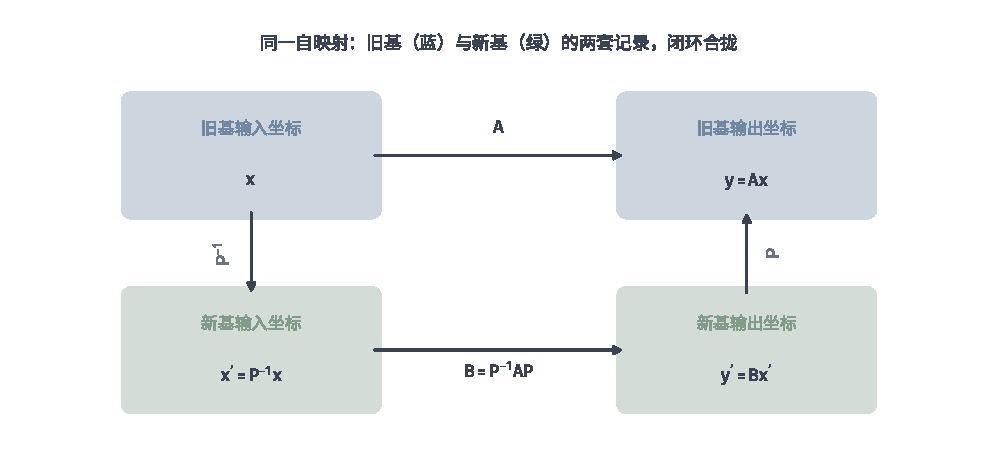
\includegraphics[width=169mm]{figures/01-mathematical-preliminaries-upper/02-linear-spaces/matplotlib/ls-similarity-change-of-basis-flow/ls-similarity-change-of-basis-flow.pdf}
  \caption{相似换基的闭环。上边是旧基下的作用$\bm y=\bm A\bm x$；左边箭头把旧输入
  坐标$\bm x$换成新输入坐标$\bm x'=\bm P^{-1}\bm x$，下边是新基下的作用
  $\bm y'=\bm B\bm x'=\bm P^{-1}\bm A\bm P\,\bm x'$，右边箭头把新输出坐标
  换回旧读数$\bm y=\bm P\bm y'$。两条路径给出同一个$\bm y$，闭环合拢即
  $\bm B=\bm P^{-1}\bm A\bm P$。}
  \label{fig:ls-similarity-change-of-basis-flow}
\end{figure*}

用一次具体换基核对对象未变，按首次阅读的顺序一步步代入。第一步选基并排换基
矩阵：在$\mathbb R^2$中取旧基为标准基，新基为$\bm b_1'=\bm e_1$、
$\bm b_2'=\bm e_1+\bm e_2$；新基向量在旧基下的坐标分别是
$(1,0)^{\top}$与$(1,1)^{\top}$，排成列得
$\bm P=\begin{bmatrix}1&1\\0&1\end{bmatrix}$，所以旧坐标$\bm x=\bm P\bm x'$，
反向为$\bm P^{-1}=\begin{bmatrix}1&-1\\0&1\end{bmatrix}$。

第二步写出旧基记录的映射。设旧矩阵为$\bm A=\begin{bmatrix}2&1\\0&3\end{bmatrix}$，
它满足$T\bm e_1=2\bm e_1$、$T\bm e_2=\bm e_1+3\bm e_2$。第三步代入公式
计算新记录：
\[
 \bm B=\bm P^{-1}\bm A\bm P
 =\begin{bmatrix}1&-1\\0&1\end{bmatrix}
 \begin{bmatrix}2&1\\0&3\end{bmatrix}
 \begin{bmatrix}1&1\\0&1\end{bmatrix}
 =\begin{bmatrix}2&0\\0&3\end{bmatrix}.
\]

两种记录对应同一个$T$：新基的两个方向$\bm e_1$与$\bm e_1+\bm e_2$正好是
$T$的两个特征方向，$T$把它们分别放大$2$倍与$3$倍，换到新基后系数可直接读出，
正是$\bm B$的对角元。改变的只是沿哪两条基方向读取，$T$本身没有被改写。

\subsubsection{性质与不变量}
\label{sec:ls-similarity-properties}

为什么先要核对相似是等价关系？换基可以做多次：不换基对应自己，换基两次可以
原路换回，两次换基可以合并成一次。具体写下来：$\bm A=\bm I^{-1}\bm A\bm I$
给出自反性；由$\bm B=\bm P^{-1}\bm A\bm P$得
$\bm A=\bm P\bm B\bm P^{-1}$给出对称性；若$\bm B=\bm P^{-1}\bm A\bm P$、
$\bm C=\bm Q^{-1}\bm B\bm Q$，则
$\bm C=(\bm P\bm Q)^{-1}\bm A(\bm P\bm Q)$给出传递性。

换基怎样搬动核与像，由这个公式直接读出。$\bm B\bm x'=\bm0$当且仅当
$\bm A(\bm P\bm x')=\bm0$，即$\bm P\bm x'\in\ker\bm A$，故
$\ker\bm B=\bm P^{-1}\ker\bm A$；同理
$\operatorname{im}\bm B=\bm P^{-1}\operatorname{im}\bm A$。核与像作为
方向集合被可逆坐标对应整体搬运，并不是逐点保持在原坐标位置。

可逆坐标对应是线性双射，保持维数，因此
\begin{equation}
 \operatorname{rank}\bm B=\operatorname{rank}\bm A,
 \qquad
 \dim\ker\bm B=\dim\ker\bm A.
 \label{eq:ls-similarity-invariants}
\end{equation}
这是本章能直接给出的相似不变量；迹与行列式在运算章定义后再核对它们的相似
不变性。

复合作用在换基下同样良好行为，这对反复作用很重要。若
$\bm B_1=\bm P^{-1}\bm A_1\bm P$、$\bm B_2=\bm P^{-1}\bm A_2\bm P$，则
\begin{equation}
 \bm B_1\bm B_2
 =\bm P^{-1}\bm A_1\bm P\,\bm P^{-1}\bm A_2\bm P
 =\bm P^{-1}\bm A_1\bm A_2\bm P.
 \label{eq:ls-similarity-product}
\end{equation}
中间的$\bm P\bm P^{-1}$抵消，复合仍表示同一对映射的复合；由此归纳得
$\bm B^k=\bm P^{-1}\bm A^k\bm P$，反复作用在新基下仍是同一过程的记录。

相应核的维数等信息保留，但一般换基不保持原坐标下的欧氏长度与夹角；长度、
夹角属于内积与度量，本章不作要求。

\subsubsection{成立条件}
\label{sec:ls-similarity-conditions}

把$\bm B=\bm P^{-1}\bm A\bm P$两端左乘$\bm P$，相似等价改写为关于
$\bm P$的方程
\begin{equation}
 \bm A\bm P=\bm P\bm B.
 \label{eq:ls-similarity-equation}
\end{equation}
这是关于$\bm P$各元素的一组线性约束。方程有非零解还不够，必须再筛出可逆解
$\det\bm P\neq0$（行列式在运算章定义）：只找到非零但奇异的$\bm P$，得到的
只是两个坐标子空间之间的对应，不是两组基之间的换基。若找到可逆$\bm P$满足
上式，则$\bm B=\bm P^{-1}\bm A\bm P$，按新基恢复出的映射与$\bm A$记录的
是同一个$T$：新坐标经$\bm B$作用后，由$\bm P$换回旧坐标恰为$\bm A$的作用。

反过来说，秩、核维数相同只给必要条件，不足以判定相似。例如$\bm I_2$与
$\begin{bmatrix}1&1\\0&1\end{bmatrix}$同秩、同核维数（核均为零），但
$\ker(\bm I_2-\bm I_2)=\mathbb R^2$与
$\ker\left(\begin{bmatrix}0&1\\0&0\end{bmatrix}\right)$维数不同，因而不相似。
检查$T$减去某个数值作用后的核维数，是比总秩更细的必要条件；完整判据需要后续
分解工具。把相似化为简单标准形的完整分类，依赖特征方向与实分裂等后续概念，在
幂序列与长期行为一节回接；本章只承诺定义层面的换基验证和已建立不变量的必要性，
不把相同秩或相同数值特征当作充分条件。

\subsection{相抵}
\label{sec:ls-equivalence-matrices}

\subsubsection{定义与含义}
\label{sec:ls-equivalence-meaning}

与同一空间上的相似对照，这里处理一般线性映射$T:V\to W$，输入空间$V$（维数$d$）
与输出空间$W$（维数$m$）是两个不同空间，各自选择自己的基，两端不必由同一个
换基矩阵联系。当$d\neq m$时甚至无法用同一个方阵同时充当两次换基，这正是相抵
比相似更一般的原因；矩阵可以是长方形$\bm A\in\mathbb R^{m\times d}$。贯穿例
$T_\varepsilon:\mathbb R^2\to\mathbb R^3$（系数映射为三个样本拟合值）正是这种两端
不同维的映射，输入端选系数基、输出端选样本读取基，各自独立。

输入端在$V$内换基，旧坐标$\bm x=\bm P\bm x'$，$\bm P$是$d\times d$可逆矩阵，
记录输入基的更换。把它代入映射$\bm y=\bm A\bm x$时，$\bm P$出现在$\bm A$的
右侧：$\bm A\bm P\bm x'$，先完成输入坐标的换算，再进入作用。输出端在$W$内
独立换基，旧坐标$\bm y=\bm Q\bm y'$，$\bm Q$是$m\times m$可逆矩阵，记录
输出基的更换。要求出新坐标$\bm y'$，就要在等式左侧用$\bm Q^{-1}$把旧输出
坐标解开，$\bm Q^{-1}$出现在$\bm A$的左侧。两端的$\bm P,\bm Q$彼此独立，
不要求对方是可逆方阵之外的任何关系。

\paragraph{相抵变换的推导}
把两次代入$\bm y=\bm A\bm x$，得$\bm Q\bm y'=\bm A\bm P\bm x'$，左乘
$\bm Q^{-1}$后
\begin{equation}
 \bm y'=\bm Q^{-1}\bm A\bm P\,\bm x',
 \qquad\text{即}\qquad
 \bm B=\bm Q^{-1}\bm A\bm P.
 \label{eq:ls-equivalence-transform}
\end{equation}
若存在实可逆$\bm Q\in\mathbb R^{m\times m}$与$\bm P\in\mathbb R^{d\times d}$
使上式成立，就称同形的$\bm A,\bm B$
\term{相抵}（equivalent matrices）。

右乘可逆$\bm P$对应输入基（列方向）的更换，左乘可逆$\bm Q^{-1}$对应输出基
（行方向）的更换。初等列变换与初等行变换分别是两端换基的具体实现，行列操作
由此获得坐标含义，不只是数表上的算术动作。

图~\ref{fig:ls-equivalence-two-sided-bases-flow}把两端独立换基的闭环画出来：
输入端经$\bm P^{-1}$换基，输出端经$\bm Q^{-1}$换基，新基下的作用$\bm B$夹在
两次回换之间。沿上边直接用$\bm A$作用，与沿下边“输入换基—作用$\bm B$—输出
回换”，殊途同归；闭环合拢的条件正是$\bm B=\bm Q^{-1}\bm A\bm P$。与
图~\ref{fig:ls-similarity-change-of-basis-flow}对照可以看出，相似是左右
两侧共用同一个$\bm P$的特例。
\begin{figure*}[htbp]
  \centering
  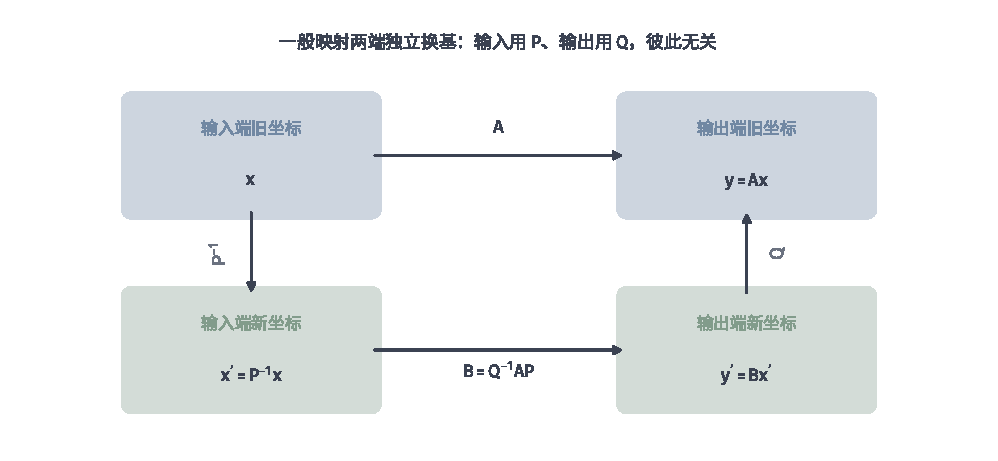
\includegraphics[width=169mm]{figures/01-mathematical-preliminaries-upper/02-linear-spaces/matplotlib/ls-equivalence-two-sided-bases-flow/ls-equivalence-two-sided-bases-flow.pdf}
  \caption{相抵两端换基的闭环。上边是旧坐标下的作用$\bm y=\bm A\bm x$；左边箭头
  把输入旧坐标$\bm x$换成新坐标$\bm x'=\bm P^{-1}\bm x$，右边箭头把输出新坐标
  $\bm y'$换回旧读数$\bm y=\bm Q\bm y'$，下边是新基下的作用
  $\bm y'=\bm B\bm x'=\bm Q^{-1}\bm A\bm P\,\bm x'$。两端的$\bm P$与$\bm Q$
  彼此独立；闭环合拢即$\bm B=\bm Q^{-1}\bm A\bm P$。}
  \label{fig:ls-equivalence-two-sided-bases-flow}
\end{figure*}

\subsubsection{性质与不变量}
\label{sec:ls-equivalence-properties}

相抵是不是等价关系，同样由公式直接核对。自反取$\bm Q=\bm I,\bm P=\bm I$得
$\bm A=\bm I^{-1}\bm A\bm I$。对称：由$\bm B=\bm Q^{-1}\bm A\bm P$，左乘
$\bm Q$、右乘$\bm P^{-1}$得$\bm A=\bm Q\bm B\bm P^{-1}$，形式仍为两端可逆
夹乘。传递：若$\bm B=\bm Q_1^{-1}\bm A\bm P_1$、
$\bm C=\bm Q_2^{-1}\bm B\bm P_2$，代入得
$\bm C=(\bm Q_1\bm Q_2)^{-1}\bm A(\bm P_1\bm P_2)$，两端可逆矩阵分别复合。

换基对核与像的影响两端各自独立。由\eqref{eq:ls-equivalence-transform}
$\bm B=\bm Q^{-1}\bm A\bm P$，$\bm B\bm x'=\bm0$等价于$\bm A\bm P\bm x'=\bm0$，
即$\bm P\bm x'\in\ker\bm A$，故$\ker\bm B=\bm P^{-1}\ker\bm A$；而
$\bm B\bm x'=\bm Q^{-1}(\bm A\bm P\bm x')$，$\bm P$遍历输入使
$\bm A\bm P\bm x'$遍历$\operatorname{im}\bm A$，$\bm Q^{-1}$再搬到输出端，
故$\operatorname{im}\bm B=\bm Q^{-1}\operatorname{im}\bm A$。核在输入端被
$\bm P$搬运，像在输出端被$\bm Q$搬运。

两次可逆坐标对应都保持维数，因此
\begin{equation}
 \operatorname{rank}\bm B=\operatorname{rank}\bm A,
 \qquad
 \dim\ker\bm B=d-\operatorname{rank}\bm A,
 \qquad
 m-\dim\operatorname{im}\bm B=m-\operatorname{rank}\bm A.
 \label{eq:ls-equivalence-invariants}
\end{equation}
保持的是两端方向的独立个数，不能宣称原坐标中的核或像逐点不动。

两端坐标独立改变，也不保留与某一端特定坐标有关的长度、角度等数值信息；相抵
比相似允许的记录变化更宽，度量由运算章的内积与范数规定。还须注意，输入与输出
是不同空间时，$\bm B$无法对自身重复作用，“复合”只发生在同一空间的自映射
之间；这是相抵与相似在对象上的根本区别。

\subsubsection{成立条件}
\label{sec:ls-equivalence-conditions}

构造判据之前，先在两端各选一组配合$T$的基。取$\ker\bm A$的一组基并扩充为
$V$的基：新增的$r$个方向在核外，它们的像线性无关（否则某一非零组合的像为零，
该组合就落进核），并恰好张成$\operatorname{im}\bm A$；在$W$中把这组$r$个
像扩充为输出基，余下的$m-r$个基方向上没有可达输出。在这样选取的输入基与输出基
下，矩阵化为秩标准形
\begin{equation}
 \begin{bmatrix}\bm I_r&\bm0\\\bm0&\bm0\end{bmatrix},
 \qquad r=\operatorname{rank}\bm A,
 \label{eq:ls-rank-normal-form}
\end{equation}
其中$r$个独立输入方向被送到$r$个独立输出方向，其余方向进核、其余输出为缺失。

\paragraph{同形同秩矩阵的相抵判据}
\begin{theorem}[相抵判据]
\label{thm:ls-equivalence-criterion}
两个同形实矩阵$\bm A,\bm B\in\mathbb R^{m\times d}$相抵，当且仅当
$\operatorname{rank}\bm A=\operatorname{rank}\bm B$。
\end{theorem}
必要性由两端可逆保持秩得到；充分性由二者都化为同一个秩标准形
\eqref{eq:ls-rank-normal-form}，两次化简连接为$\bm Q^{-1}\bm A\bm P$。固定
形状之后，秩就是相抵的完整不变量。设$\bm A,\bm B$都化到同一秩标准形$\bm R$：
$\bm R=\bm Q_A^{-1}\bm A\bm P_A=\bm Q_B^{-1}\bm B\bm P_B$。两式对接得
$\bm B=\bm Q_B\bm Q_A^{-1}\bm A\bm P_A\bm P_B^{-1}$，对照
\eqref{eq:ls-equivalence-transform}即解出$\bm Q=\bm Q_A\bm Q_B^{-1}$、
$\bm P=\bm P_A\bm P_B^{-1}$。具体用哪些消元或分解把矩阵化到标准形，算法在
求解章建立，这里只给出对接关系。退化边界也由此清楚：零秩对应零映射，
$\bm A=\bm0$只能与零矩阵相抵；满行秩时输出全部可达，满列秩时核为零。同秩
但不同形状的矩阵不直接比较，相抵以同形为前提。

\subsection{合同}
\label{sec:ls-congruence}

\subsubsection{定义与含义}
\label{sec:ls-congruence-meaning}

前两种关系记录单输入算子；合同记录的是把两个向量位置分别读成一个数的规则。
\term{双线性型}（bilinear form）是在两个输入位置上分别保持线性组合的规则
$B:V\times V\to\mathbb R$，即$B(a\bm u+b\bm u',\bm v)=aB(\bm u,\bm v)+bB(\bm u',\bm v)$，
另一位置同理。在选定基下它写成$B(\bm u,\bm v)=\bm u^{\top}\bm A\bm v$，矩阵
$\bm A$记录这次读取：$A_{i,j}=B(\bm b_i,\bm b_j)$。例如$B(\bm u,\bm v)=u_1v_2$
由$\bm A=\begin{bmatrix}0&1\\0&0\end{bmatrix}$记录，对象不是一个自映射，
$\bm A$乘的是两个变量而不是把一个向量送到另一个向量。

双线性型的两个位置都取自同一个空间$V$，因此换基时两个位置使用同一组变量、
同一次坐标更换：$\bm u=\bm P\bm x$，$\bm v=\bm P\bm y$，$\bm P$是同一个
可逆换元矩阵，而不是左右各取一个。这与相抵形成对照：相抵的输入、输出是两个空间，
两侧可以分别换基；合同只在一个空间内换元，若给两个位置各配一个不同矩阵，就是在
两套互不相干的坐标里读取同一个型，不再记录换元前后的同一个$B$。

\paragraph{合同变换的推导}
代入得
\begin{equation}
 B(\bm P\bm x,\bm P\bm y)
 =\bm x^{\top}\bm P^{\top}\bm A\bm P\,\bm y,
 \qquad\text{即}\qquad
 \bm C=\bm P^{\top}\bm A\bm P.
 \label{eq:ls-congruence-transform}
\end{equation}
若存在实可逆$\bm P$使上式成立，就称$\bm A$与$\bm C$
\term{合同}（congruent）。合同本身不要求$\bm A$对称。

把两个位置取成同一个变量，$q_A(\bm x)=\bm x^{\top}\bm A\bm x$称为
\term{二次型}（quadratic form）。
只有对称部分$\bm S=(\bm A+\bm A^{\top})/2$出现在$q_A$中：
$\bm x^{\top}\bm A\bm x=\bm x^{\top}\bm S\bm x$，反对称部分取值恒为零。
一般双线性型与其二次型不能混同，非对称矩阵的反对称信息在对角取值中消失。合同与
相似的对象也由此分清：合同记录同一个二次型或双线性读取在换元下的表达，变换是
$\bm P^{\top}$；相似记录同一个自映射在换基下的表达，变换是$\bm P^{-1}$。
即使形式上都乘可逆矩阵，二者回答的问题不同。

\subsubsection{性质与不变量}
\label{sec:ls-congruence-properties}

合同是不是等价关系，由$\bm C=\bm P^{\top}\bm A\bm P$核对。自反取
$\bm P=\bm I$得$\bm A=\bm I^{\top}\bm A\bm I$。对称：两边乘
$\bm P^{-\top}$与$\bm P^{-1}$（其中$\bm P^{-\top}=(\bm P^{-1})^{\top}$），
得$\bm A=\bm P^{-\top}\bm C\bm P^{-1}$。传递：若
$\bm C=\bm P_1^{\top}\bm A\bm P_1$、$\bm D=\bm P_2^{\top}\bm C\bm P_2$，
代入得$\bm D=(\bm P_1\bm P_2)^{\top}\bm A(\bm P_1\bm P_2)$，两个可逆
换元复合后仍可逆。

换元怎样改变二次型的取值，是合同真正要回答的问题。由
$q_C(\bm y)=\bm y^{\top}\bm C\bm y
=(\bm P\bm y)^{\top}\bm A(\bm P\bm y)=q_A(\bm P\bm y)$，
可逆换元把$q_A$在$\bm P\bm y$方向上的取值搬到$q_C$在$\bm y$方向上。因为
$\bm P$可逆，$\bm y\neq\bm0$当且仅当$\bm P\bm y\neq\bm0$，于是
$q_A(\bm P\bm y)>0$、$=0$、$<0$分别对应$q_C(\bm y)>0$、$=0$、$<0$；
数值大小随换元改变，正负号与零值方向双向对应保持。

对所有非零$\bm x$都有$q_A(\bm x)>0$时称\term{正定}（positive definite），
$q_A(\bm x)\geq0$时称\term{半正定}（positive semidefinite），既取正值又取
负值时称\term{不定}（indefinite）。可逆换元下正、负、零值方向双向对应，
因此这些符号性质保持；以使二次型严格为正或严格为负的最大子空间维数，以及
$\dim\ker\bm A$，记录符号结构，它们都经可逆换元给出的线性双射保持不变，
秩也因$\bm P$可逆而保持。这里用二次型本身判断符号，不借用尚未建立的谱分类。

还须区分两类“零”：$q_A(\bm x)=0$不等于$\bm A\bm x=\bm0$。例如$q=x^2-y^2$
在$(1,1)^{\top}$上取值为零，但$\operatorname{diag}(1,-1)$可逆、核为零；
零能量方向不是核方向，不能从某个方向的零能量判定零惯性。

\subsubsection{成立条件}
\label{sec:ls-congruence-conditions}

验证两个矩阵合同，就是寻找可逆$\bm P$使$\bm C=\bm P^{\top}\bm A\bm P$；这是
关于$\bm P$元素的一组方程，可逆性是合法换元的前提。秩相同只给出必要条件：可逆
$\bm P$保秩，合同必有同秩，但同秩不足以判定合同，例如$\operatorname{diag}(1,1)$
与$\operatorname{diag}(1,-1)$同秩，正负方向个数不同，并不合同。能直接配方的
例子可以当场看出符号：$x^2+2xy+y^2=(x+y)^2$恒非负、在$x+y=0$上取零，是
半正定；$x^2-y^2=(x+y)(x-y)$在$(1,0)$取正、在$(0,1)$取负，是不定；
$x^2$只取非负且仅在$x=0$取零。配方把二次型拆成若干带符号的平方项，可逆换元
不改变正、负平方项的个数，故配方直接处理的符号结构在可逆换元下保持。

实对称矩阵合同的完整判据（正负零方向个数相同，即惯性三元组）需要把正、负、零方向
化为相同标准坐标，其构造在二次优化一节以谱为工具完成；本章只由可逆对应证明符号
子空间维数保持，不提前用特征值定义惯性或承诺完整分类。同惯性的充要分类也不扩大
到任意非对称矩阵：反对称部分不出现在二次型中，非对称双线性型不能套用实对称型的
判据；正定情形只含正方向，因此同阶正定二次型彼此合同。

\section{本章小结}
\label{sec:ls-representation-summary}

本章回答“怎样表示”，得到一条由对象到记录的链条。4.1先辨认标量、向量、矩阵与
张量：对象本身不是一串数，数只是选定方向以后的记录。4.2把可相加、可缩放的对象
规定为实线性空间，张成回答表示能否存在，线性无关回答表示是否唯一，二者共同给出
基与不依赖选择的维数。4.3研究同一环境中子空间的包含、交、和与直和，维数公式
\eqref{eq:ls-dimension-formula}由公共基扩充得到，一般补空间不是正交补。

4.4固定有序基建立坐标，并区分被动换基与主动作用。4.5把保持线性组合的对应记录为
矩阵，用核、像与秩零度定理\eqref{eq:ls-rank-nullity}计数被消去与被保留的
自由度，据此判断单射、满射与可逆性。4.6把标量读取规则收集为对偶空间，对偶映射
以转置表示，并由此证明行秩等于列秩。4.7以差属于子空间定义等价类，商空间消去指定
方向，且$V/\ker T\cong\operatorname{im}T$。

4.8比较三种换记录关系：相似$\bm B=\bm P^{-1}\bm A\bm P$记录同一自映射，
相抵$\bm B=\bm Q^{-1}\bm A\bm P$记录两端独立换基的同一映射，合同
$\bm C=\bm P^{\top}\bm A\bm P$记录同一双线性读取；三者对象不同，保持的
不变量也不同，且本章只用秩与核维数。

仅有坐标尚未指定长度、夹角或最优性：度量配对与范数在运算章建立，反求未知量在
求解章按目标判存在唯一，结果对数据与计算误差的敏感度在分析章衡量。贯穿例
$\bm X_\varepsilon$的近共线结构，将在这些章节依次回到拟合稳定而系数敏感的
现象。

\chapter{运算}
\label{chap:linear-operations}

第~\ref{chap:linear-representation}章把标量、向量、矩阵和映射用基与坐标记录下来。记录本身不回答“怎样算”：两个预测分支的输出怎样合并，两个映射怎样先后作用，一个数组换一种排列后哪些量改变，怎样判断两个方向是否垂直，一个误差向量究竟算多大，一组向量张成的体积有多大，多轴数据又怎样组合与汇总。本章在实数、有限维范围内逐一规定这些基本运算：每种运算说明它做什么、输入输出满足什么条件，以及可以直接使用的性质。第~\ref{chap:sets-functions-and-proofs}章已经给出逐项加减、数乘和行列相乘的算式，这里不重复算术教程。

运算按作用分为三组。第一组把对象合并成同类对象：加法与数乘（\ref{sec:ls-addition-scaling}），逐项乘法、矩阵乘法以及由反复相乘得到的矩阵幂（\ref{sec:ls-multiplication}），还有只改变记录位置的转置与重排（\ref{sec:ls-reshaping}）。第二组给对象以几何：内积把两个对象配成标量并规定垂直（\ref{sec:ls-inner-products}），范数为对象给出大小（\ref{sec:ls-norms-distances}），伴随把内积配对中的作用从一侧搬到另一侧（\ref{sec:ls-adjoints}）。第三组处理多个槽位：外积与行列式测量一组向量张成的有向体积（\ref{sec:ls-exterior-determinants}），张量积、Kronecker积与缩约组织多轴数据的组合与汇总（\ref{sec:ls-tensor-operations}）。

% 第5章：加法与数乘、乘法（逐项乘法、矩阵乘法、矩阵幂）、转置与重排、内积、范数与距离、伴随。

\section{加法与数乘}
\label{sec:ls-addition-scaling}

第~\ref{chap:sets-functions-and-proofs}章已经按对应坐标定义了向量、矩阵的逐项相加与实数数乘，第~\ref{sec:ls-vector-spaces}节又把这些规则抽象为线性空间公理。本节不再重复逐项算式，只回答两个实际问题：两个对象或两个映射在什么条件下可以相加，以及按结构组织计算时实际付出多少。

\subsection{定义与性质}

两个数组能够相加，首先要求形状相同、对应索引的含义相同：$\bm A,\bm B\in\mathbb R^{m\times n}$才有$(\bm A+\bm B)_{i,j}=a_{i,j}+b_{i,j}$，向量$\bm x,\bm y\in\mathbb R^d$才有$(\bm x+\bm y)_j=x_j+y_j$。形状不同的数组不能逐项配对；即使元素总数恰好相同，把$m\times n$与$p\times q$直接相加也没有定义，因为第$(i,j)$个位置在两张表中可能记录不同的量。数乘$c\bm A$把每个元素乘以同一个实数$c$，不改变形状。

逐项规则只用到实数加法与乘法，因此第~\ref{sec:ls-vector-spaces}节列出的交换律、结合律、零元与负元、数乘分配律都按位置各自成立，不需要新的验证。需要单独记住的是相容条件：$\bm A+\bm B$合法当且仅当两者属于同一个同型数组空间。

\paragraph{线性组合与张成}
\label{sec:linear-algebra-map-addition}

若干同型对象分别乘以系数后相加，就是它们的\term{线性组合}：$\sum_{j=1}^k c_j\bm A_j$的每个位置是对应位置元素的同一组合。系数$c_j$是实数，不要求非负，也不要求和为$1$；固定一组系数，线性组合把多个记录合并成一个同型记录。

映射也可以叠加。设$T,S:V\to W$是同一对空间之间的两个线性映射，定义
\[
 (aT+bS)(\bm x)=aT\bm x+bS\bm x,\qquad \bm x\in V,
\]
其中$a,b\in\mathbb R$。叠加保持线性：把输入的线性组合代入，两个分支分别展开再汇总即可。在$V$与$W$的固定基下，$T,S$的矩阵为$\bm A,\bm B$，则$aT+bS$的矩阵就是$a\bm A+b\bm B$。

相加的前提是两个映射的定义域与陪域都一致。这并不要求$V=W$：两个从$\mathbb R^2$到$\mathbb R^3$的映射照样可以相加，只是不能与一个从$\mathbb R^3$到$\mathbb R^2$的映射相加。系数$a,b$必须与输入无关；若叠加系数随$\bm x$改变，叠加后的映射一般不再线性，需要单独检验。

\section{乘法}
\label{sec:ls-multiplication}

“相乘”在线性代数里有两种互不相同的含义。逐项乘法在对应位置把两个同形数组配对相乘，不汇总任何索引；矩阵乘法把两个映射经中间空间复合，对被消去的索引求和。二者输入条件、输出形状和线性性都不同。同一个方阵与自身反复复合得到矩阵幂，它是矩阵乘法的特例，放在本节最后。

\subsection{逐项乘法}

\subsubsection{定义与性质}

\paragraph{逐项乘积（Hadamard积）}

设$\bm A,\bm B\in\mathbb R^{m\times n}$，\term{逐元素乘积}（Hadamard product）记作$\bm A\odot\bm B$，定义为
\begin{equation}
 (\bm A\odot\bm B)_{i,j}=a_{i,j}b_{i,j},
 \label{eq:ls-hadamard}
\end{equation}
输出仍是$m\times n$，每个位置只取两个因子在同一位置的数相乘，不对任何索引求和。例如
\[
 \begin{bmatrix}1&2\\3&4\end{bmatrix}
 \odot
 \begin{bmatrix}0&1\\1&0\end{bmatrix}
 =
 \begin{bmatrix}0&2\\3&0\end{bmatrix}.
\]
它适合表达“用一个掩码挑选或调制另一个数组”：固定掩码$\bm M$后，$\bm X\mapsto\bm M\odot\bm X$把$\bm M$为零的位置置零，把非零位置按系数缩放。

由于等式~\eqref{eq:ls-hadamard} 右端只是实数乘法，按位置逐项验证即得交换律$\bm A\odot\bm B=\bm B\odot\bm A$、结合律$(\bm A\odot\bm B)\odot\bm C=\bm A\odot(\bm B\odot\bm C)$，以及对加法的分配律$\bm A\odot(\bm B+\bm C)=\bm A\odot\bm B+\bm A\odot\bm C$；单位元是全$1$数组。固定一个因子时$\bm X\mapsto\bm M\odot\bm X$是线性映射；两个因子都作为未知量时，乘积只对各自分别线性：同时把两者放大两倍，结果放大四倍。

逐项乘积不是映射复合。上面两个矩阵的普通乘积是$\begin{smallmatrix}2&1\\4&3\end{smallmatrix}$，与逐项结果完全不同。逐项乘法还依赖所选坐标：换基后同一对象的坐标改变，原掩码位置不再对应原来的方向。因此它描述的是记录层面的配对，而矩阵乘法对应与坐标无关的映射复合。

\subsection{矩阵乘法}

\subsubsection{定义与含义}

矩阵乘法来自映射的复合。设$T:U\to V$、$S:V\to W$是线性映射，先让$\bm x$经过$T$得到中间结果$\bm y=T\bm x\in V$，再让$S$作用于$\bm y$，得到$S(T\bm x)\in W$。复合$S\circ T$从$U$直接到$W$，中间空间$V$只用于衔接。

在固定基下设$\bm y=\bm B\bm x$（$\bm B\in\mathbb R^{d\times k}$），$\bm z=\bm A\bm y$（$\bm A\in\mathbb R^{m\times d}$）。逐坐标展开
\[
 z_i=\sum_{\ell=1}^d a_{i,\ell}y_\ell
 =\sum_{\ell=1}^d a_{i,\ell}\sum_{j=1}^k b_{\ell,j}x_j
 =\sum_{j=1}^k\left(\sum_{\ell=1}^d a_{i,\ell}b_{\ell,j}\right)x_j.
\]
有限求和交换次序后，中间坐标$y_\ell$被消去，$z_i$直接由$x_j$表示。

\paragraph{矩阵乘法的定义}

对相容形状的$\bm A\in\mathbb R^{m\times d}$、$\bm B\in\mathbb R^{d\times k}$，乘积$\bm A\bm B\in\mathbb R^{m\times k}$定义为
\begin{equation}
 (\bm A\bm B)_{i,j}=\sum_{\ell=1}^d a_{i,\ell}b_{\ell,j}.
 \label{eq:linear-algebra-matrix-product}
\end{equation}
左矩阵的列数必须等于右矩阵的行数，这个公共维数就是被消去的中间空间维数；第$(i,j)$项取左矩阵第$i$行与右矩阵第$j$列逐项相乘再相加。按行乘列不是任意约定，而是“先代入再读出”这一复合要求的唯一写法。

同一乘积有三种读法。按列看，$(\bm A\bm B)_{:,j}=\bm A\bm B_{:,j}$：$\bm A$作用在$\bm B$的每一列上，乘积记录$\bm B$的各列再经$\bm A$传播的结果。按行看，$(\bm A\bm B)_{i,:}=\bm A_{i,:}\bm B$：$\bm B$作用在$\bm A$的每一行上。按中间索引看，
\begin{equation}
 \bm A\bm B=\sum_{\ell=1}^d\bm A_{:,\ell}\bm B_{\ell,:},
 \label{eq:ls-product-outer-sum}
\end{equation}
乘积是$d$个秩一矩阵之和，每个中间维度贡献一项。三种读法给出同一组数，区别在于先汇总哪个索引，这决定了后面的分块与近似方式。

规则$\bm x\mapsto\bm A\bm x+\bm b$在$\bm b\neq\bm0$时是仿射映射而不是线性映射，因为它把$\bm0$送到$\bm b$。两个仿射映射$\bm x\mapsto\bm A_1\bm x+\bm b_1$、$\bm y\mapsto\bm A_2\bm y+\bm b_2$复合得$\bm x\mapsto\bm A_2\bm A_1\bm x+(\bm A_2\bm b_1+\bm b_2)$，平移项也被后一个映射作用。给坐标补一个恒为$1$的末位，仿射映射可以写成增广空间上的线性作用：
\begin{equation}
 \begin{bmatrix}\bm A&\bm b\\ \bm0^\top&1\end{bmatrix}
 \begin{bmatrix}\bm x\\1\end{bmatrix}
 =
 \begin{bmatrix}\bm A\bm x+\bm b\\1\end{bmatrix}.
 \label{eq:ls-affine-homogeneous}
\end{equation}
大矩阵对整个增广空间是线性的，但原输入被限制在末坐标为$1$的集合上，不能据此声称原映射线性；复合仿射映射对应增广矩阵的普通乘积。

\subsubsection{运算性质}
\label{sec:linear-algebra-map-composition}

映射复合满足结合律：$(R\circ S)\circ T$与$R\circ(S\circ T)$都是先$T$、再$S$、后$R$。翻译成矩阵即$(\bm A\bm B)\bm C=\bm A(\bm B\bm C)$，可在式~\eqref{eq:linear-algebra-matrix-product} 中交换有限求和次序验证，所以多个相容矩阵连乘不需要规定括号。复合也保持叠加：$\bm A(\bm B+\bm C)=\bm A\bm B+\bm A\bm C$，$(\bm A+\bm B)\bm C=\bm A\bm C+\bm B\bm C$，$c(\bm A\bm B)=(c\bm A)\bm B=\bm A(c\bm B)$。单位矩阵满足$\bm I_m\bm A=\bm A=\bm A\bm I_d$，对应恒等映射。

复合次序不能交换。先交换坐标再保留第一坐标，与先保留第一坐标再交换，结果不同：
\[
 \begin{bmatrix}1&0\\0&0\end{bmatrix}
 \begin{bmatrix}0&1\\1&0\end{bmatrix}
 =
 \begin{bmatrix}0&1\\0&0\end{bmatrix},\qquad
 \begin{bmatrix}0&1\\1&0\end{bmatrix}
 \begin{bmatrix}1&0\\0&0\end{bmatrix}
 =
 \begin{bmatrix}0&0\\1&0\end{bmatrix}.
\]
一般$\bm A\bm B\neq\bm B\bm A$，书写乘积时必须从右向左读作用顺序。

乘积可以为零而两个因子都不为零：取$\bm A=\begin{smallmatrix}1&0\\0&0\end{smallmatrix}$、$\bm B=\begin{smallmatrix}0&0\\1&0\end{smallmatrix}$，则$\bm A\bm B=\bm0$。$\bm A\bm B=\bm0$恰好意味着$\bm B$的每一列都落入$\bm A$的零空间，即$\operatorname{range}(\bm B)\subseteq\operatorname{null}(\bm A)$：右因子的可达方向被左因子完全消去，因此不能由$\bm A\bm B=\bm0$推出某个因子为零。

把矩阵按行、列分成尺寸相容的小块，乘法规则对块照样成立：$\bm C_{i,j}=\sum_\ell\bm A_{i,\ell}\bm B_{\ell,j}$，其中$\bm A_{i,\ell}$的列数须等于$\bm B_{\ell,j}$的行数。例如把中间维数分成两段，$\bm C_{i,j}=\bm A_{i,1}\bm B_{1,j}+\bm A_{i,2}\bm B_{2,j}$，与整段求和逐项相等。这称为分块矩阵乘法，块可以像数一样参与运算，只是块之间的次序不能交换。

由第~\ref{sec:ls-injective-surjective-invertible}节的可逆判定，方阵乘积$\bm A\bm B$可逆当且仅当$\bm A$与$\bm B$都可逆，且$(\bm A\bm B)^{-1}=\bm B^{-1}\bm A^{-1}$：先作用的后撤销。

\subsection{矩阵幂}
\label{sec:ls-matrix-powers}
\label{sec:ch06-powers-spectrum}

同一个方阵反复作用，是矩阵乘法最常见的特例：定常迭代$\bm x^{(k+1)}=\bm A\bm x^{(k)}$走$k$步后得到$\bm x^{(k)}=\bm A^k\bm x^{(0)}$。

\paragraph{定义与运算规则}

矩形矩阵不能与自身复合，幂只对$d$阶方阵定义：$\bm A^k$是$k$个$\bm A$连乘（$k\geq1$），并规定$\bm A^0=\bm I_d$，表示不施加任何作用；$\bm A$可逆时再定义负幂$\bm A^{-k}=(\bm A^{-1})^k$。幂是作用的反复复合，不是逐元素乘方：$\bm A=\begin{pmatrix}1&1\\0&1\end{pmatrix}$给出$\bm A^2=\begin{pmatrix}1&2\\0&1\end{pmatrix}$，非对角元随复合次数累加。

由结合律，同一矩阵的幂满足$\bm A^m\bm A^n=\bm A^{m+n}$、$(\bm A^m)^n=\bm A^{mn}$（指数在有定义的范围内取整数），不同次幂彼此交换。不同矩阵则不然：$(\bm B\bm C)^2=\bm B\bm C\bm B\bm C$只有在$\bm B\bm C=\bm C\bm B$时才能整理成$\bm B^2\bm C^2$。例如$\bm B=\begin{pmatrix}0&1\\0&0\end{pmatrix}$、$\bm C=\begin{pmatrix}1&0\\1&0\end{pmatrix}$给出$(\bm B\bm C)^2=\begin{pmatrix}1&0\\0&0\end{pmatrix}$，而$\bm B^2\bm C^2=\bm0$。

两类幂关系经常出现。满足$\bm A^2=\bm A$的作用称为\term{幂等}（idempotent），施加一次与施加多次效果相同，把向量投到某个子空间上的投影就是这种作用。存在正整数$s$使$\bm N^s=\bm0$的作用称为\term{幂零}（nilpotent），它在有限步后把所有向量送到零；例如$\bm N=\begin{pmatrix}0&1\\0&0\end{pmatrix}\neq\bm0$，却有$\bm N^2=\bm0$。

\paragraph{特征值与特征向量}
\label{sec:matrix-analysis-spectrum}

直接连乘会不断混合坐标，$\bm A^k$的长期样子难以从元素看出。第~\ref{sec:ls-operator-eigenvectors}节的特征向量给出简化：
由$\bm A\bm v=\lambda\bm v$归纳得$\bm A^k\bm v=\lambda^k\bm v$，沿特征方向，$k$次作用化为标量乘方，长度乘以$|\lambda|^k$，
$\lambda<0$时每次还翻转方向。例如$\bm A=\begin{pmatrix}0.8&4\\0&0.5\end{pmatrix}$满足$\bm A(1,0)^\top=0.8(1,0)^\top$与
$\bm A(-40/3,1)^\top=0.5(-40/3,1)^\top$，两条特征方向上的分量分别按$0.8^k$与$0.5^k$衰减。

若$\bm A$实可对角化，把$d$个线性无关的特征向量排成可逆矩阵$\bm V$，则$\bm A\bm V=\bm V\bm\Lambda$，即
$\bm A=\bm V\bm\Lambda\bm V^{-1}$，其中$\bm\Lambda$是特征值组成的对角矩阵；于是$\bm A^k=\bm V\bm\Lambda^k\bm V^{-1}$，
幂只需对对角元逐个乘方。并非每个实方阵都可对角化：$\begin{pmatrix}0.8&1\\0&0.8\end{pmatrix}$的特征向量只有$(1,0)^\top$的倍数，
凑不出两条独立方向，其幂中会出现$k\,0.8^{k-1}$这样的项。特征值怎样求出、何时可以对角化，要借助第~\ref{sec:ls-determinant-properties}节的行列式回答。

\section{转置与重排}
\label{sec:ls-reshaping}
\label{sec:linear-algebra-tensors-structured-operations}

加法与乘法都产生新的数值；还有一类操作只改变元素记录在哪个位置，不对任何索引求和，也不改变元素数值。转置、轴置换、reshape与向量化都属于这一类，使用前必须说清新索引怎样对应旧索引。

\subsection{索引变换}

转置交换行与列：若$\bm A\in\mathbb R^{m\times n}$，则$\bm A^\top\in\mathbb R^{n\times m}$满足$(\bm A^\top)_{j,i}=a_{i,j}$。每个元素原样搬到新位置，形状交换而数值不变。

对多于两个轴的数组，\term{维度重排}（permutation of axes）按给定顺序调换轴的位置。例如$y_{i,k,j}=x_{i,j,k}$把$b\times\ell\times d$的数组变为$b\times d\times\ell$：第一个轴保持原位，第二、第三轴互换。元素跟随自己的索引移动，轴的含义不变，只是记录次序改变。

\term{形状重整}（reshape）先指定元素的遍历顺序，再把同一个数列装入另一形状，仅要求元素总数相同。以
$\bm A=\begin{smallmatrix}1&2&3\\4&5&6\end{smallmatrix}$为例，轴交换得到
$\bm A^\top=\begin{smallmatrix}1&4\\2&5\\3&6\end{smallmatrix}$，而按行读取后重整成$3\times2$得到
$\begin{smallmatrix}1&2\\3&4\\5&6\end{smallmatrix}$，两者不同。所以重整不能只给目标形状，还要给遍历顺序；形状相同不能说明完成了轴交换。

图~\ref{fig:vol1-add-linear-transpose-reshape} 把两种结果并排放置：转置后原两行分别成为两列，按行重整则把数列$1,2,3,4,5,6$依次装入新表，原来相邻的元素被安排到不同位置。
\begin{figure}[!htb]
  \centering
  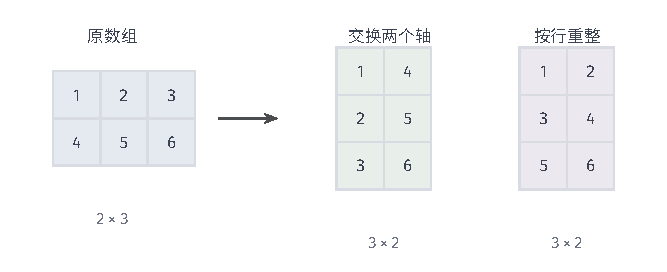
\includegraphics[width=112mm]{figures/01-mathematical-preliminaries-upper/02-linear-spaces/tikz/comprehension-additions/linear-transpose-reshape.pdf}
  \caption{轴交换与按行重整。原数组两行为$(1,2,3)$与$(4,5,6)$；中图转置后两列分别保留原来的两行，右图则把按行读取的数列$1,2,3,4,5,6$依次装入$3\times2$数组。数字及其排列由正文示例直接给出。}
  \label{fig:vol1-add-linear-transpose-reshape}
\end{figure}

\paragraph{向量化}

按列堆叠的\term{向量化}（vectorization）把$m\times n$矩阵展成长列：
\[
 \operatorname{vec}(\bm A)=(a_{1,1},\ldots,a_{m,1},a_{1,2},\ldots,a_{m,n})^\top,
\]
元素$a_{i,j}$对应一维索引$i+(j-1)m$。反过来，矩阵展开（unfolding）把多维数组的指定轴选为行、其余轴合并为列，得到一个矩阵；选哪些轴保留为独立索引，决定展开结果的形状，也决定后续乘积汇总哪个轴。向量化与展开都是固定索引映射的reshape，保留全部信息。

\subsection{运算性质}

目标形状与遍历顺序固定后，转置、轴置换、reshape与向量化都是数组空间之间的线性双射：它们把加法和数乘逐项搬到新排列，逆变换（再转置一次、逆置换、按原次序装回）恢复原数组。因此$(\bm A+\bm B)^\top=\bm A^\top+\bm B^\top$、$(c\bm A)^\top=c\bm A^\top$一类等式按位置直接成立。

转置与乘法的交互由元素公式推出：
\[
 (\bm A^\top)^\top=\bm A,\qquad
 (\bm A\bm B)^\top=\bm B^\top\bm A^\top,\qquad
 (\bm A^{-1})^\top=(\bm A^\top)^{-1}.
\]
乘积转置后因子次序反转；可逆矩阵转置后仍可逆，逆与转置可交换次序。转置还保持矩阵秩，因为行空间与列空间只是互换。一般reshape不保持矩阵秩：它只重排元素，新矩阵各行各列之间的线性相关关系可以完全不同。轴置换与reshape都不是映射作用，把存储格式当成几何性质或变换效果，是这里最常见的错误。

\section{内积}
\label{sec:ls-inner-products}

加法与乘法回答怎样合并对象，内积则把两个对象配成一个标量：它同时给出长度、角度和垂直的判据。第~\ref{chap:sets-functions-and-proofs}章已在标准坐标下定义$\langle\bm x,\bm y\rangle=\sum_j x_jy_j$，本节先把它抽象为配对公理，再引入区分方向代价的加权配对，最后用Gram矩阵建立正交分解和线性泛函的内积表示。

\subsection{内积的定义与性质}

\paragraph{内积的定义}

\begin{definition}[实内积]
\label{def:linear-algebra-inner-product}
\label{def:functional-inner-product-space}
实向量空间$V$上的\term{内积}（inner product）是映射$\langle\cdot,\cdot\rangle:V\times V\to\mathbb R$，同时满足下列三条公理。
\begin{enumerate}
 \item 双线性：对两个变量分别保持线性组合，即$\langle a\bm x+b\bm y,\bm z\rangle=a\langle\bm x,\bm z\rangle+b\langle\bm y,\bm z\rangle$，且对第二变量同样线性。
 \item 对称性：$\langle\bm x,\bm y\rangle=\langle\bm y,\bm x\rangle$。
 \item 正定性：$\langle\bm x,\bm x\rangle>0$对所有非零$\bm x$成立，且$\langle\bm x,\bm x\rangle=0$当且仅当$\bm x=\bm0$。
\end{enumerate}
配备内积的向量空间称为\term{内积空间}（inner-product space）。
\end{definition}

标准实坐标的内积是$\langle\bm x,\bm y\rangle=\bm x^\top\bm y=\sum_j x_jy_j$。由配对直接诱导长度
\begin{equation}
 \lVert\bm x\rVert=\sqrt{\langle\bm x,\bm x\rangle},
 \label{eq:linear-algebra-inner-product-norm}
\end{equation}
$\langle\bm x,\bm y\rangle=0$时称两向量\term{正交}（orthogonal）。

\paragraph{Cauchy--Schwarz不等式}

内积能否给出夹角，取决于配对值是否受两个长度控制。
\begin{theorem}[Cauchy--Schwarz不等式]
\label{thm:linear-algebra-cauchy-schwarz}
在内积空间中，$|\langle\bm x,\bm y\rangle|\leq\lVert\bm x\rVert\,\lVert\bm y\rVert$，等号成立当且仅当两向量线性相关。
\end{theorem}
\begin{proof}
$\bm y=\bm0$时两边都为零。否则令$a=\langle\bm x,\bm y\rangle/\lVert\bm y\rVert^2$，则
\[
 0\leq\lVert\bm x-a\bm y\rVert^2
 =\lVert\bm x\rVert^2-\frac{\langle\bm x,\bm y\rangle^2}{\lVert\bm y\rVert^2}.
\]
移项即得不等式；等号恰好要求$\bm x-a\bm y=\bm0$，即两向量共线。
\end{proof}

非零向量的夹角由$\cos\theta=\langle\bm x,\bm y\rangle/(\lVert\bm x\rVert\lVert\bm y\rVert)$定义，CS不等式保证它落在$[-1,1]$。例如$\bm x=(1,0)^\top$、$\bm y_\varepsilon=(1,\varepsilon)^\top$随$\varepsilon\to0$趋近共线，
\begin{equation}
 \cos\theta_\varepsilon=\frac{1}{\sqrt{1+\varepsilon^2}}\longrightarrow1,
 \label{eq:linear-algebra-nearly-collinear-angle}
\end{equation}
这给“几乎同向”一个确定的欧氏度量；更换内积也会更换角度。

并非每个范数都来自内积。实向量空间中一个范数来自内积，当且仅当它满足\term{平行四边形恒等式}
\begin{equation}
 \lVert\bm x+\bm y\rVert^2+\lVert\bm x-\bm y\rVert^2
 =2\lVert\bm x\rVert^2+2\lVert\bm y\rVert^2.
 \label{eq:functional-parallelogram-identity}
\end{equation}
必要性由内积展开直接得到；例如第~\ref{sec:ls-norms-distances}节的$\ell_1$范数在$\bm e_1,\bm e_2$上左侧为$8$、右侧为$4$，故不来自任何内积。充分性可用极化公式$\langle\bm x,\bm y\rangle=(\lVert\bm x+\bm y\rVert^2-\lVert\bm x-\bm y\rVert^2)/4$恢复配对，这里不展开。

对同形矩阵，把元素看作有限坐标，得到\term{Frobenius内积}
\[
 \langle\bm A,\bm B\rangle_{\mathrm F}=\sum_{i,j}a_{i,j}b_{i,j},
 \qquad
 \lVert\bm A\rVert_{\mathrm F}=\left(\sum_{i,j}a_{i,j}^2\right)^{1/2}.
\]
这是矩阵作为数表本身的长度；它与矩阵作为变换时的最大放大率不是同一口径，后者在第~\ref{sec:ls-matrix-norms}节建立。

\subsection{加权内积}
\label{sec:ls-weighted-inner-products}

标准坐标把每个方向一视同仁，但实际问题里不同方向的代价不同。设$\bm M=\operatorname{diag}(4,1)$，则$\sqrt{4x_1^2+x_2^2}$把第一坐标的偏差放大两倍：点$(1,1)$的欧氏长度是$\sqrt2$，这种加权长度却是$\sqrt5$。只要权重矩阵满足适当条件，这样的长度仍来自一个合法内积。

对称矩阵$\bm M$给出二次型$q(\bm x)=\bm x^\top\bm M\bm x$：若对每个非零$\bm x$都有$q(\bm x)>0$，称$\bm M$\term{正定}（positive definite）；若只保证$q(\bm x)\geq0$，称$\bm M$\term{半正定}（positive semidefinite）。要求对称，是因为配对必须对称；非对称部分在$\bm x^\top\bm M\bm x$中自动抵消，不进入二次型。

\paragraph{加权内积的定义}

对称正定$\bm M$给出加权配对
\[
 \langle\bm x,\bm y\rangle_{\bm M}=\bm x^\top\bm M\bm y,
 \qquad
 \lVert\bm x\rVert_{\bm M}=\sqrt{\bm x^\top\bm M\bm x}.
\]
它满足双线性、对称与正定性，是一个合法内积。若$\bm M$仅半正定，配对只给半内积，诱导半范数以及伪距离
\begin{equation}
 d_{\bm M}(\bm x,\bm y)
 =\sqrt{(\bm x-\bm y)^\top\bm M(\bm x-\bm y)}.
 \label{eq:linear-algebra-mahalanobis-pseudodistance}
\end{equation}
不同点的距离可能为零：例如$\bm M=\operatorname{diag}(1,0)$无法区分$(0,0)^\top$与$(0,1)^\top$。半正定时CS不等式仍可由$\langle\bm x+t\bm y,\bm x+t\bm y\rangle_{\bm M}\geq0$对所有实数$t$成立得到，三角不等式保留。

\paragraph{Gram因子定理}

加权配对不必当作新几何：有限维半正定矩阵都能写成欧氏平方和。
\begin{theorem}[半正定矩阵的配方因子]
\label{thm:ls-gram-factor}
设$\bm M\in\mathbb R^{r\times r}$对称半正定，则存在$\bm L$使$\bm M=\bm L^\top\bm L$；若$\bm M$正定，可取$\bm L$可逆。
\end{theorem}
\begin{proof}
对$r$归纳。$r=1$时$\bm M=(m_{1,1})$且$m_{1,1}\geq0$，取$\bm L=(\sqrt{m_{1,1}})$即可。

若所有对角项都为零，任取$i,j$，把$\bm x=\bm e_i+t\bm e_j$代入半正定性：
\[
 0\leq\bm x^\top\bm M\bm x=2t\,m_{i,j}+t^2m_{j,j}=2t\,m_{i,j},
\]
对正负$t$同时成立迫使$m_{i,j}=0$，于是$\bm M=0$，取$\bm L=0$。

否则存在正对角项。取一个置换矩阵$\bm P$（行列同步交换，$\bm P^\top=\bm P^{-1}$）把它换到首位，记
\[
 \widetilde{\bm M}=\bm P\bm M\bm P^\top
 =\begin{bmatrix}a&\bm b^\top\\ \bm b&\bm C\end{bmatrix},\qquad a>0.
\]
配方消去第一行：令$\bm x=(-\bm b^\top\bm u/a,\bm u)$，则$\bm x^\top\widetilde{\bm M}\bm x=\bm u^\top(\bm C-\bm b\bm b^\top/a)\bm u\geq0$，故余项$\bm M'=\bm C-\bm b\bm b^\top/a$仍半正定。由归纳假设$\bm M'=\bm L'^\top\bm L'$，取上三角因子
\[
 \widetilde{\bm L}=\begin{bmatrix}\sqrt a&\bm b^\top/\sqrt a\\ \bm0&\bm L'\end{bmatrix},
\]
直接相乘得
\[
 \widetilde{\bm L}^\top\widetilde{\bm L}
 =\begin{bmatrix}a&\bm b^\top\\ \bm b&\bm b\bm b^\top/a+\bm L'^\top\bm L'\end{bmatrix}
 =\widetilde{\bm M}.
\]
换回原矩阵：$\bm M=\bm P^\top\widetilde{\bm M}\bm P=(\widetilde{\bm L}\bm P)^\top(\widetilde{\bm L}\bm P)$，取$\bm L=\widetilde{\bm L}\bm P$即可。

正定时$\bm M'$也正定（上述$\bm x$在$\bm u\neq\bm0$时非零），归纳得$\bm L'$可逆，于是$\widetilde{\bm L}$可逆，$\bm L=\widetilde{\bm L}\bm P$仍可逆。
\end{proof}
于是加权长度可写成$\lVert\bm x\rVert_{\bm M}=\lVert\bm L\bm x\rVert_2$：正定时只是换了一组坐标，退化时则把$\bm L$的零空间方向压成零长度。使用半内积前必须先说明哪些方向被忽略，不能把退化配对当成正定内积参与正交判断。证明中的配方步骤就是第~\ref{sec:ls-exact-linear-equations}节Cholesky分解的雏形。

对两个对称矩阵记$\bm M\succeq\bm N$当且仅当$\bm M-\bm N$半正定，即$\bm x^\top\bm M\bm x\geq\bm x^\top\bm N\bm x$对所有$\bm x$成立，它给出加权长度的逐点比较$\lVert\bm x\rVert_{\bm M}\geq\lVert\bm x\rVert_{\bm N}$。作可逆线性替换$\bm x=\bm S\bm z$，二次型变为$\bm z^\top(\bm S^\top\bm M\bm S)\bm z$；这种合同变换$\bm M\mapsto\bm S^\top\bm M\bm S$保持半正定性、正定性与序关系。因此换基后新坐标下的度量矩阵是$\bm S^\top\bm M\bm S$而不是$\bm M$，把新坐标直接按欧氏长度比较，一般已经换了问题。

\subsection{正交关系}
\label{sec:ls-orthogonality}

\paragraph{Gram矩阵}

正交是两个向量之间的关系；一组向量之间的全部配对关系由一张数表记录。
\begin{definition}[有限向量族的Gram矩阵]
\label{def:linear-algebra-gram-matrix}
向量$\bm b_1,\ldots,\bm b_r$的\term{Gram矩阵}（Gram matrix）为$g_{i,j}=\langle\bm b_i,\bm b_j\rangle$。若$\bm B$以它们为列，标准坐标中$\bm G=\bm B^\top\bm B$，加权坐标中$\bm G=\bm B^\top\bm M\bm B$。
\end{definition}

因为$\bm a^\top\bm G\bm a=\lVert\sum_j a_j\bm b_j\rVert^2\geq0$，Gram矩阵半正定；并且$\bm G$正定（从而非奇异）当且仅当这组向量线性无关：线性相关时某个非零系数使组合为零，平方长度为零；线性无关时任意非零系数的组合非零，平方长度为正。$\bm G$是对角阵恰好表示这组向量两两正交，是单位阵则表示两两正交且长度为$1$。图~\ref{fig:ls-gram-matrix-coefficients} 把两条基向量的两两内积排成数表。
\begin{figure}[!htb]
  \centering
  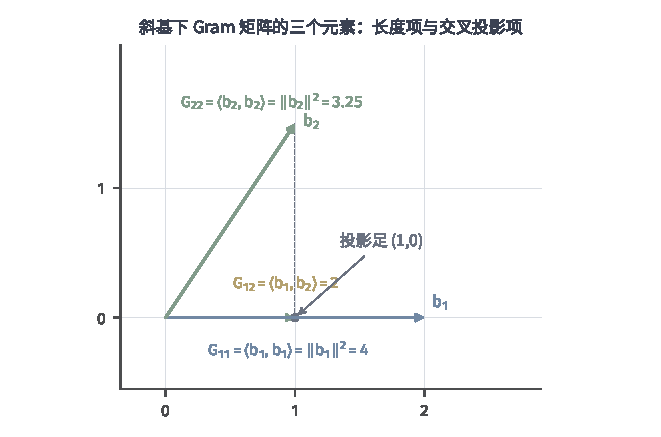
\includegraphics[width=112mm]{figures/01-mathematical-preliminaries-upper/02-linear-spaces/matplotlib/ls-gram-matrix-coefficients/ls-gram-matrix-coefficients.pdf}
  \caption{Gram矩阵把一组基向量的两两内积排成数表。左：平面上两条不垂直的基向量$\bm b_1,\bm b_2$及其夹角；右：$G_{i,j}=\langle\bm b_i,\bm b_j\rangle$构成的$2\times2$Gram矩阵，对角元为各向量长度平方，非对角元为夹角投影。基越接近正交，非对角元越接近零；线性相关时$\det\bm G=0$。向量与矩阵均为解析教学例。}
  \label{fig:ls-gram-matrix-coefficients}
\end{figure}

\paragraph{正交补与正交直和}

设$U$是有限维内积空间$V$的子空间，\term{正交补}（orthogonal complement）定义为
\[
 U^\perp=\{\bm r\in V:\langle\bm u,\bm r\rangle=0,\ \forall\bm u\in U\}.
\]
Gram矩阵非奇异给出正交分解的存在与唯一。
\begin{lemma}[正交直和]
\label{lem:ls-orthogonal-decomposition}
设$U$是有限维内积空间$V$的子空间，则每个$\bm x\in V$唯一分解为$\bm x=\bm u+\bm r$，其中$\bm u\in U$、$\bm r\in U^\perp$；即$V=U\oplus U^\perp$。
\end{lemma}
\begin{proof}
取$U$的一组基$\bm b_1,\ldots,\bm b_r$，其Gram矩阵$\bm G$非奇异。对任意$\bm x$，令$\bm u=\sum_j a_j\bm b_j$，并要求$\bm r=\bm x-\bm u$与每个$\bm b_i$正交，得到系数方程
\[
 \sum_j g_{i,j}a_j=\langle\bm b_i,\bm x\rangle,\qquad i=1,\ldots,r,
\]
即$\bm G\bm a=(\langle\bm b_i,\bm x\rangle)_i$。非奇异$\bm G$保证系数唯一解出，残差$\bm r$与全部基向量正交，因而落在$U^\perp$。

若$\bm x=\bm u+\bm r=\bm u'+\bm r'$是两种分解，则$\bm u-\bm u'=\bm r'-\bm r$同时属于$U$与$U^\perp$，与自身正交，长度为零，故两种分解相同。
\end{proof}
这里只证明正交分量存在且唯一；它就是$U$中离$\bm x$最近的点，这一判定与具体算法在第~\ref{sec:ls-subspace-nearest-points}节给出。

\section{范数与距离}
\label{sec:ls-norms-distances}
\label{sec:linear-algebra-distance-relations}
\label{sec:ch06-map-comparison}
\label{sec:matrix-analysis-norms-effective-rank}
\label{sec:linear-algebra-length-angle-distance}

同一个误差向量$(1,1)$可以按绝对偏差计为$2$，按欧氏长度计为$\sqrt2$，也可以只记录最大坐标偏差$1$。不同任务要求不同的误差含义，没有对所有目的都最合适的长度。本节用范数统一表达这些尺度，再给出矩阵的大小、点间的距离与夹角，以及线性读取在给定误差预算下的最大值。

\subsection{向量范数}

\paragraph{范数的定义}

\begin{definition}[赋范空间]
\label{def:functional-normed-space}
设$V$为实向量空间。映射$\lVert\cdot\rVert:V\to[0,\infty)$同时满足下列四条公理时，称为\term{范数}（norm），$(V,\lVert\cdot\rVert)$称为\term{赋范空间}（normed space）。它诱导距离$d(\bm x,\bm y)=\lVert\bm x-\bm y\rVert$。
\begin{enumerate}
 \item 非负性：$\lVert\bm x\rVert\geq0$。
 \item 正定性：$\lVert\bm x\rVert=0$当且仅当$\bm x=\bm0$。
 \item 齐次性：$\lVert c\bm x\rVert=|c|\,\lVert\bm x\rVert$。
 \item 三角不等式：$\lVert\bm x+\bm y\rVert\leq\lVert\bm x\rVert+\lVert\bm y\rVert$。
\end{enumerate}
\end{definition}

内积诱导的$\lVert\bm x\rVert=\sqrt{\langle\bm x,\bm x\rangle}$满足公理：正定性直接来自内积，三角不等式由$\lVert\bm x+\bm y\rVert^2=\lVert\bm x\rVert^2+2\langle\bm x,\bm y\rangle+\lVert\bm y\rVert^2$和CS不等式得到。

有限坐标中常用
\[
 \lVert\bm x\rVert_p=\left(\sum_j|x_j|^p\right)^{1/p}\quad(1\leq p<\infty),
 \qquad
 \lVert\bm x\rVert_\infty=\max_j|x_j|.
\]
$p=1$累加绝对偏差，$p=2$累计平方偏差再开方，$p=\infty$控制最大坐标偏差。图~\ref{fig:ls-norm-unit-balls} 比较三种口径下单位球的形状。
\begin{figure*}[htbp]
  \centering
  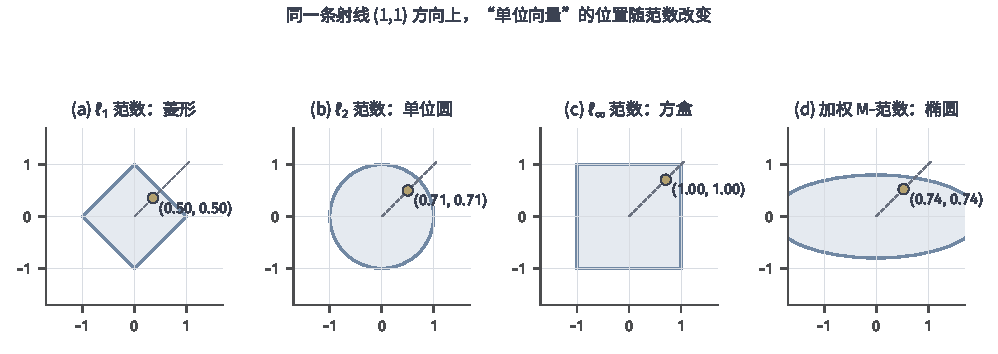
\includegraphics[width=169mm]{figures/01-mathematical-preliminaries-upper/02-linear-spaces/matplotlib/ls-norm-unit-balls/ls-norm-unit-balls.pdf}
  \caption{同一向量在不同范数下的“单位球”形状。左：$\ell_1$单位球为菱形（累加绝对偏差）；中：$\ell_2$单位球为圆（欧氏长度）；右：$\ell_\infty$单位球为正方形（最大坐标偏差）。同一个点$(1,1)$的范数依次为$2$、$\sqrt2$、$1$，单位球大小随口径而变，三者之间的倍数关系由正文的显式不等式给出。三图坐标尺度相同，为解析教学例。}
  \label{fig:ls-norm-unit-balls}
\end{figure*}

$p=1,2,\infty$的三角不等式可以直接验证；一般$p$需要下面的不等式。
\begin{theorem}[有限维Hölder不等式]
\label{thm:linear-algebra-holder}
设$1\leq p,q\leq\infty$且$1/p+1/q=1$（约定$1/\infty=0$），则$|\bm x^\top\bm y|\leq\lVert\bm x\rVert_p\lVert\bm y\rVert_q$。
\end{theorem}
\begin{proof}
先设$1<p,q<\infty$。Young不等式$uv\leq u^p/p+v^q/q$对$u,v\geq0$成立：$u>0$时令$t=v/u^{p-1}$，验证$1/p+t^q/q-t\geq0$，其最小值在$t=1$处为零；$u=0$时也成立。两向量非零时取$u_j=|x_j|/\lVert\bm x\rVert_p$、$v_j=|y_j|/\lVert\bm y\rVert_q$求和，得$\sum_j u_jv_j\leq1/p+1/q=1$，恢复尺度后用$|\bm x^\top\bm y|\leq\sum_j|x_j||y_j|$。零向量时两侧都为零；$p=1,q=\infty$时用$\sum_j|x_j||y_j|\leq(\max_j|y_j|)\sum_j|x_j|$，另一端点交换两者。
\end{proof}
对一般$p$，把$|x_j+y_j|^{p}\leq|x_j+y_j|^{p-1}(|x_j|+|y_j|)$求和后对两部分分别应用Hölder，得到
$\lVert\bm x+\bm y\rVert_p^p\leq(\lVert\bm x\rVert_p+\lVert\bm y\rVert_p)\lVert\bm x+\bm y\rVert_p^{p-1}$，非零时相除即得三角不等式（Minkowski不等式）。常用坐标范数之间还有直接界
\[
 \lVert\bm x\rVert_\infty\leq\lVert\bm x\rVert_2\leq\sqrt d\,\lVert\bm x\rVert_\infty,
 \qquad
 \lVert\bm x\rVert_2\leq\lVert\bm x\rVert_1\leq\sqrt d\,\lVert\bm x\rVert_2,
\]
右端两式分别来自$\sum_jx_j^2\leq d\max_jx_j^2$与Cauchy--Schwarz不等式。维数增大时$\sqrt d$不能在误差预算中忽略。

分组误差要先固定分组方式，例如以行为组的混合范数
$\lVert\bm A\rVert_{p,q}=(\sum_i\lVert\bm A_{i,:}\rVert_p^q)^{1/q}$，内层衡量组内、外层汇总各组。允许非零对象也具有零大小、但保留齐次性与三角不等式的尺度称为\term{半范数}（seminorm），它给出伪距离：例如只读取截距的仿射函数尺度$p(f_{a,b})=|a|$忽略全部斜率方向，相同截距的不同函数距离为零。把零方向归并为同一元素后得到的商范数，在讨论点到子空间的距离时给出（第~\ref{sec:ls-quotient-norms}节）。

\subsection{矩阵范数}
\label{sec:ls-matrix-norms}

矩阵有两种“大小”口径：Frobenius范数描述数表本身有多大；误差分析更关心它作为变换最坏把输入放大多少倍。
\begin{definition}[由向量范数诱导的矩阵范数]
\label{def:matrix-analysis-induced-norm}
给定输入范数$\lVert\cdot\rVert_\alpha$和输出范数$\lVert\cdot\rVert_\beta$，\term{诱导矩阵范数}（induced matrix norm）为
\[
 \lVert\bm A\rVert_{\alpha\to\beta}
 =\sup_{\bm x\neq0}\frac{\lVert\bm A\bm x\rVert_\beta}{\lVert\bm x\rVert_\alpha}.
\]
两端采用同一类$p$范数时简写为$\lVert\bm A\rVert_p$。
\end{definition}

\paragraph{诱导矩阵范数}

由定义直接得$\lVert\bm A\bm x\rVert_\beta\leq\lVert\bm A\rVert_{\alpha\to\beta}\lVert\bm x\rVert_\alpha$，诱导范数就是这一不等式中最小的常数。标准坐标下两个诱导范数可直接读取：
\[
 \lVert\bm A\rVert_1=\max_j\sum_i|a_{i,j}|,\qquad
 \lVert\bm A\rVert_\infty=\max_i\sum_j|a_{i,j}|.
\]
第一式由$\lVert\bm A\bm x\rVert_1\leq\sum_j|x_j|\lVert\bm A_{:,j}\rVert_1$得到上界，在最大绝对列和对应的坐标向量上达到；第二式的上界同理，取输入各坐标为对应行元素的符号即达到。诱导$2$范数也称\term{谱范数}（spectral norm），$\lVert\bm A\rVert_2=\sup_{\lVert\bm x\rVert_2=1}\lVert\bm A\bm x\rVert_2$；对每行用CS不等式得$\lVert\bm A\bm x\rVert_2\leq\lVert\bm A\rVert_{\mathrm F}\lVert\bm x\rVert_2$，故它有限且$\lVert\bm A\rVert_2\leq\lVert\bm A\rVert_{\mathrm F}$，其奇异值表达在第~\ref{sec:ls-svd}节推导。对一般的范数对，比值有界且上确界在某个方向达到，由第~\ref{sec:ls-error-scale-comparison}节的范数等价与极值定理保证。图~\ref{fig:ls-induced-norm-action} 把单位圆被拉成椭圆后的最长轴读作最大放大倍数。
\begin{figure*}[htbp]
  \centering
  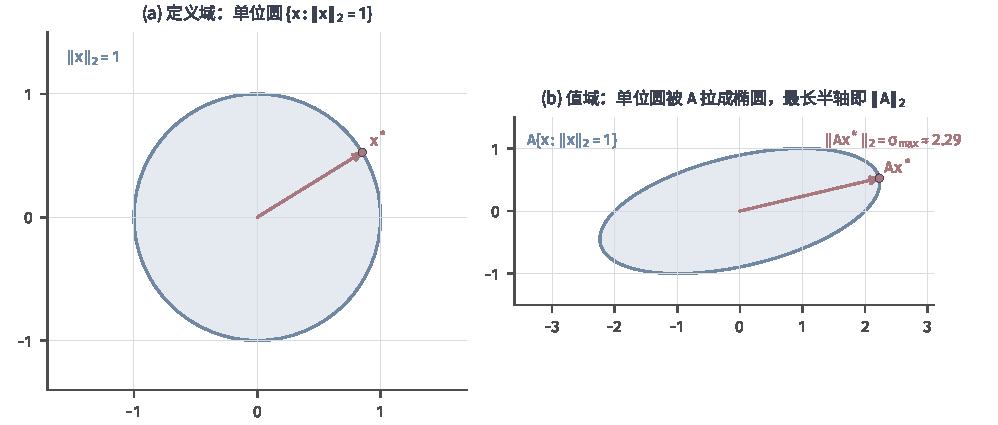
\includegraphics[width=169mm]{figures/01-mathematical-preliminaries-upper/02-linear-spaces/matplotlib/ls-induced-norm-action/ls-induced-norm-action.pdf}
  \caption{诱导矩阵范数衡量最坏放大倍数。左：单位圆$\lVert\bm x\rVert_2=1$；中：同一线性作用$\bm A$把单位圆映成椭圆；右：椭圆上最长的轴给出$\lVert\bm A\rVert_2=\max_{\lVert\bm x\rVert_2=1}\lVert\bm A\bm x\rVert_2$，箭头指示最大放大方向。数值由$\bm A$的教学构造直接得到，是解析例。}
  \label{fig:ls-induced-norm-action}
\end{figure*}

Frobenius范数从另一个角度累计作用：
\[
 \lVert\bm A\rVert_{\mathrm F}^2
 =\sum_j\lVert\bm A\bm e_j\rVert_2^2
 =\sum_{i,j}a_{i,j}^2,
\]
它是所有标准输入方向的总平方输出，而非一次最坏输入。对$\bm A=\begin{smallmatrix}1&1\\0&1\end{smallmatrix}$，$\lVert\bm A\rVert_1=\lVert\bm A\rVert_\infty=2$、$\lVert\bm A\rVert_{\mathrm F}=\sqrt3$，不同口径的数值不必相同。

中间空间范数匹配时，连续应用两次界得到次乘性
\[
 \lVert\bm A\bm B\rVert_{\alpha\to\gamma}
 \leq\lVert\bm A\rVert_{\beta\to\gamma}
 \lVert\bm B\rVert_{\alpha\to\beta}.
\]
逐列应用诱导范数界，转置后对列重复同一论证，得到混合界
\begin{equation}
 \lVert\bm A\bm B\rVert_{\mathrm F}
 \leq\lVert\bm A\rVert_2\lVert\bm B\rVert_{\mathrm F},
 \qquad
 \lVert\bm A\bm B\rVert_{\mathrm F}
 \leq\lVert\bm A\rVert_{\mathrm F}\lVert\bm B\rVert_2.
 \label{eq:matrix-analysis-mixed-submultiplicativity}
\end{equation}
其中$\lVert\bm B^\top\rVert_2=\lVert\bm B\rVert_2$可由
$\lVert\bm B\rVert_2=\max_{\lVert\bm x\rVert_2=\lVert\bm y\rVert_2=1}|\bm y^\top\bm B\bm x|$交换两向量得到。结合$\lVert\bm A\rVert_2\leq\lVert\bm A\rVert_{\mathrm F}$，Frobenius范数也次乘。

\subsection{距离与夹角}

范数诱导的距离$d(\bm x,\bm y)=\lVert\bm x-\bm y\rVert$满足非负、对称与三角不等式；非零向量的夹角已由CS不等式在第~\ref{sec:ls-inner-products}节定义。更换范数只改变距离口径，不改变两点是否重合。

比较两个方向时先把各自归一化到单位长度，消除整体缩放：$\bm x$与$c\bm x$（$c\neq0$）是同一方向，$\langle\bm x/\lVert\bm x\rVert,\bm y/\lVert\bm y\rVert\rangle$才只反映角度。两个子空间之间的夹角以各自单位向量之间的最小夹角为起点定义，其计算与敏感度在后续分析章节展开。尺度约定不同（例如一边用$\ell_2$、一边用$\ell_1$又不归一）时，比较结果没有意义，因此先统一度量口径再谈远近。

\subsection{对偶范数}
\label{sec:ls-dual-norms}

\paragraph{对偶范数}

误差$\bm r$只知道落在某个范数球内时，一次线性读取$\bm z^\top\bm r$最多变化多少，由下面的量回答。
\begin{definition}[对偶范数]
\label{def:linear-algebra-dual-norm}
给定$\mathbb R^d$上的范数，相对于标准坐标配对的\term{对偶范数}（dual norm）为
\begin{equation}
 \lVert\bm z\rVert_*=\sup_{\lVert\bm r\rVert\leq1}|\bm z^\top\bm r|.
 \label{eq:linear-algebra-dual-norm-definition}
\end{equation}
\end{definition}
它满足范数公理：线性读取满足三角不等式与齐次性，非零$\bm z$总能读取某个坐标得到非零值。对$\ell_p$范数，下面直接构造达到上确界的$\bm r$；一般范数下上确界同样可以取到（第~\ref{sec:ls-error-scale-comparison}节）。图~\ref{fig:ls-dual-norm-unit-ball} 把这个最大值画成支撑线最后接触单位球的位置。

\begin{figure}[!htb]
  \centering
  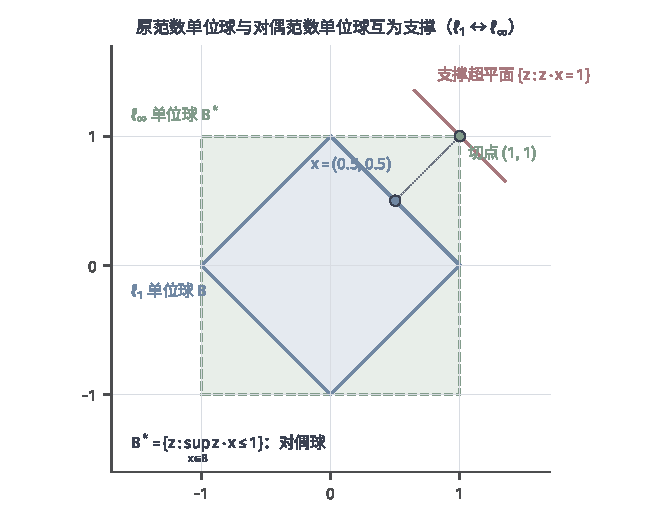
\includegraphics[width=112mm]{figures/01-mathematical-preliminaries-upper/02-linear-spaces/matplotlib/ls-dual-norm-unit-ball/ls-dual-norm-unit-ball.pdf}
  \caption{对偶范数的几何：在原范数单位球$\lVert\bm r\rVert\leq1$上求线性读取$\bm z^\top\bm r$的最大值。左：原单位球（灰色）与读取方向$\bm z$；右：支撑直线最后接触单位球处给出$\lVert\bm z\rVert_*=\max_{\lVert\bm r\rVert\leq1}|\bm z^\top\bm r|$。对偶单位球（虚线）与原单位球互为极体，为解析教学例。}
  \label{fig:ls-dual-norm-unit-ball}
\end{figure}

Hölder不等式给出$\ell_p$单位球上的上界$\lVert\bm z\rVert_q$，且上界可达到：$1<p<\infty$时取$r_j=|z_j|^{q-1}\operatorname{sgn}(z_j)/\lVert\bm z\rVert_q^{q-1}$；$p=1$时把单位预算放在$|z_j|$最大的坐标；$p=\infty$时逐坐标取$r_j=\operatorname{sgn}(z_j)$。因而
\begin{equation}
 (\lVert\cdot\rVert_p)_*=\lVert\cdot\rVert_q,\qquad \frac1p+\frac1q=1,
 \label{eq:linear-algebra-lp-duality}
\end{equation}
并对$\rho\geq0$有
\begin{equation}
 \max_{\lVert\bm r\rVert_p\leq\rho}|\bm z^\top\bm r|
 =\rho\lVert\bm z\rVert_q.
 \label{eq:linear-algebra-linear-perturbation-duality}
\end{equation}
例如$\bm z=(2,-1)^\top$、$|r_j|\leq0.01$时最大变化为$0.03$，由$\bm r=(0.01,-0.01)^\top$达到。图~\ref{fig:linear-algebra-dual-unit-balls} 固定同一次读取，显示预算形状怎样改变最坏方向。
\begin{figure*}[htbp]
  \centering
  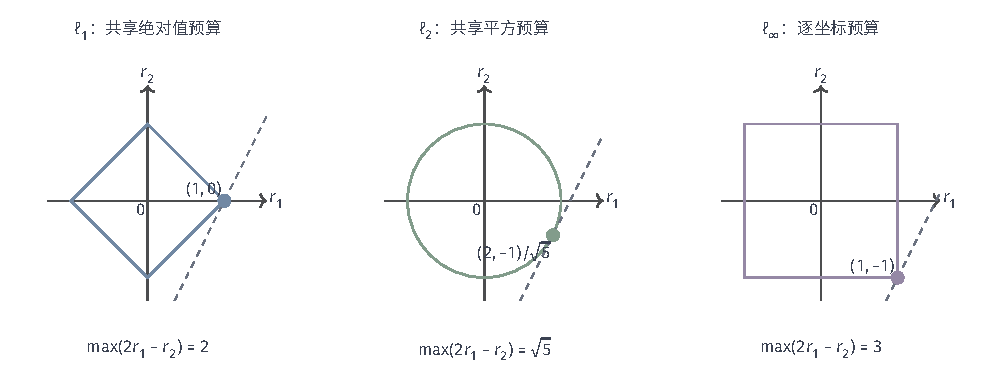
\includegraphics[width=168.998mm]{figures/01-mathematical-preliminaries-upper/02-linear-spaces/tikz/linear-algebra-dual-unit-balls/figure.pdf}
  \caption{同一线性读取$2r_1-r_2$在$\ell_1$、$\ell_2$、$\ell_\infty$单位球上的最大值依次为$2$、$\sqrt5$、$3$。虚线为最后接触可行集的支撑直线，点为最大化方向。三图坐标尺度相同，均为解析教学例；改变允许误差的形状会改变误差常数。}
  \label{fig:linear-algebra-dual-unit-balls}
\end{figure*}

加权长度$\lVert\bm r\rVert_{\bm M}=\sqrt{\bm r^\top\bm M\bm r}$的对偶范数由逆矩阵给出：误差按$\bm M$计量时，读取方向要按$\bm M^{-1}$计量。
\begin{theorem}[加权对偶范数]
\label{prop:ls-weighted-dual-norm}
设$\bm M$对称正定，则范数$\lVert\cdot\rVert_{\bm M}$相对于标准坐标配对的对偶范数为
\[
 \lVert\bm z\rVert_{\bm M,*}
 =\sup_{\bm r^\top\bm M\bm r\leq1}\bm z^\top\bm r
 =\sqrt{\bm z^\top\bm M^{-1}\bm z}.
\]
\end{theorem}
\begin{proof}
取可逆配方因子$\bm M=\bm L^\top\bm L$（定理~\ref{thm:ls-gram-factor}），令$\bm w=\bm L\bm r$，约束化为$\bm w^\top\bm w\leq1$，目标化为$\bm z^\top\bm r=\bm z^\top\bm L^{-1}\bm w=(\bm L^{-\top}\bm z)^\top\bm w$。由欧氏情形$\sup_{\lVert\bm w\rVert_2\leq1}\bm a^\top\bm w=\lVert\bm a\rVert_2$（$\bm w=\bm a/\lVert\bm a\rVert_2$时取到），上确界为
\[
 \lVert\bm L^{-\top}\bm z\rVert_2
 =\sqrt{\bm z^\top\bm L^{-1}\bm L^{-\top}\bm z}
 =\sqrt{\bm z^\top\bm M^{-1}\bm z},
\]
其中$\bm L^{-1}\bm L^{-\top}=(\bm L^\top\bm L)^{-1}=\bm M^{-1}$。
\end{proof}

把约束中的$\bm r$按比例缩放，定理也可写成$\bm z^\top\bm M^{-1}\bm z=\sup_{\bm r\neq\bm0}(\bm z^\top\bm r)^2/(\bm r^\top\bm M\bm r)$。由这一极值写法立即得到正定矩阵求逆的序反转。
\begin{theorem}[正定求逆的序反转]
\label{cor:ls-inverse-order-reversal}
若$\bm M_1\preceq\bm M_2$都正定，则$\bm M_2^{-1}\preceq\bm M_1^{-1}$。
\end{theorem}
\begin{proof}
对任意$\bm z$，由$\bm r^\top\bm M_1\bm r\leq\bm r^\top\bm M_2\bm r$，分母较小者比值较大：
\[
 \bm z^\top\bm M_2^{-1}\bm z
 =\sup_{\bm r\neq\bm0}\frac{(\bm z^\top\bm r)^2}{\bm r^\top\bm M_2\bm r}
 \leq\sup_{\bm r\neq\bm0}\frac{(\bm z^\top\bm r)^2}{\bm r^\top\bm M_1\bm r}
 =\bm z^\top\bm M_1^{-1}\bm z.
\]
\end{proof}
原度量增大时，对偶度量缩小。这是两个对称矩阵之间的序关系，不是逐元素不等式。

\section{伴随}
\label{sec:ls-adjoints}

矩阵转置把作用从输出端搬回输入端，但“搬运”依赖所选配对。内积空间中这个搬运者称为伴随；它与代数对偶中的转置、与求解复原的逆是三个不同对象。

\subsection{定义与性质}

\paragraph{内积伴随的定义}

设$T:V\to W$是两个有限维实内积空间之间的线性映射。若存在$T^\star:W\to V$使
\begin{equation}
 \langle T\bm x,\bm y\rangle_W=\langle\bm x,T^\star\bm y\rangle_V
 \label{eq:ls-adjoint-pairing}
\end{equation}
对所有$\bm x\in V$、$\bm y\in W$成立，则$T^\star$称为$T$的\term{伴随}（adjoint）。
\label{def:linear-algebra-adjoint}

伴随总存在且唯一。取$V,W$的基，把两边的内积写成$\langle\bm x,\bm x'\rangle_V=\bm x^\top\bm M_V\bm x'$、$\langle\bm y,\bm y'\rangle_W=\bm y^\top\bm M_W\bm y'$，其中$\bm M_V,\bm M_W$是基的Gram矩阵，对称正定因而可逆；设$T$的矩阵为$\bm A$，所求伴随的矩阵为$\bm B$。式~\eqref{eq:ls-adjoint-pairing}要求$(\bm A\bm x)^\top\bm M_W\bm y=\bm x^\top\bm M_V\bm B\bm y$对所有$\bm x,\bm y$成立，即$\bm A^\top\bm M_W=\bm M_V\bm B$，它有唯一解
\begin{equation}
 \bm B=\bm M_V^{-1}\bm A^\top\bm M_W.
 \label{eq:ls-weighted-adjoint}
\end{equation}
标准内积下$\bm M_V,\bm M_W$都是单位矩阵，伴随矩阵就是$\bm A^\top$；两边权重不同时，伴随既不是单纯转置，也不是转置再求逆。

伴随与组合的规则由配对定义逐项推出：
\[
 (T+S)^\star=T^\star+S^\star,\qquad
 (cT)^\star=c\,T^\star,\qquad
 (TS)^\star=S^\star T^\star,\qquad
 T^{\star\star}=T.
\]
复合伴随的次序与乘积转置一样反转；恒等映射的伴随是自身。图~\ref{fig:ls-adjoint-action-transfer} 把这种配对方向的搬回画成示意图。
\begin{figure}[!htb]
  \centering
  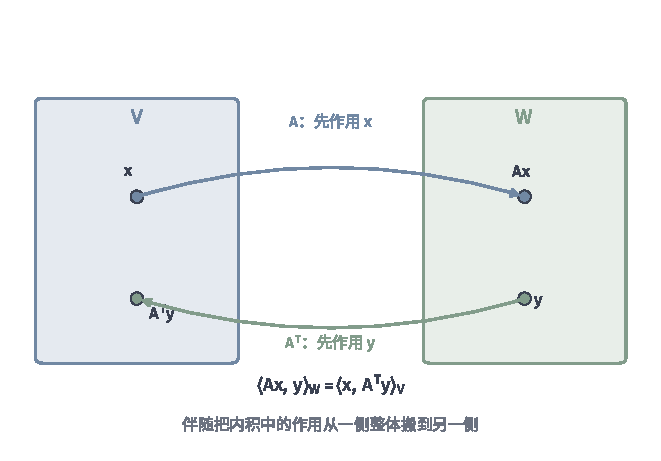
\includegraphics[width=112mm]{figures/01-mathematical-preliminaries-upper/02-linear-spaces/matplotlib/ls-adjoint-action-transfer/ls-adjoint-action-transfer.pdf}
  \caption{内积伴随把输出端的配对搬回输入端。左：$T:V\to W$把$\bm x$映成$T\bm x$，与$\bm y\in W$配对；右：伴随$T^\star:W\to V$把$\bm y$映回$T^\star\bm y\in V$，使$\langle T\bm x,\bm y\rangle_W=\langle\bm x,T^\star\bm y\rangle_V$。标准欧氏内积下$T^\star$就是转置，是配对方向的反转而非逆作用。箭头与空间为解析示意。}
  \label{fig:ls-adjoint-action-transfer}
\end{figure}

标准欧氏内积下伴随就是矩阵转置，因此转置是伴随在一种特定配对下的特例；更换加权内积后伴随一般不等于转置，见式~\eqref{eq:ls-weighted-adjoint}。第~\ref{sec:ls-dual-spaces}节从代数对偶出发的转置记录的是线性泛函的坐标变换，不需要内积。伴随也不是逆：逆把输出复原成输入，伴随只把读取方向换一侧。例如$2I$的伴随仍是$2I$，而逆为$\tfrac12 I$。

若$T^\star=T$，称$T$为\term{自伴}（self-adjoint），标准坐标下对应对称矩阵。若$Q^\star Q=I$，称$Q$为\term{正交}（orthogonal）作用：它保持内积$\langle Q\bm x,Q\bm y\rangle=\langle\bm x,Q^\star Q\bm y\rangle=\langle\bm x,\bm y\rangle$，在方阵情形下$Q^{-1}=Q^\star$。满足$TT^\star=T^\star T$的作用称为\term{正规}（normal）作用，自伴与正交都属于它；这些类别的谱性质在后续谱分解中展开，这里只给出定义。

% ============================================================
% 第5章：外积与行列式、张量运算（张量积、Kronecker积、张量缩约）、本章小结
% ============================================================

\section{外积与行列式}
\label{sec:ls-exterior-determinants}
\label{sec:linear-algebra-scalar-readouts}

内积回答一个向量有多长、两个向量夹角多大；把一组向量看成一个整体，还需要测量它们张成的平行多面体有多大。平行四边形的面积、平行六面体的体积都不是逐对长度相加能得到的量：它们由向量之间的相对方向共同决定，并且在两个向量交换位置时改变指向。本节先用一种满足交替性的多线性乘法建立外积，再在最高维得到行列式，说明它怎样测量体积缩放、怎样判断退化，以及怎样把特征值问题化为一个多项式方程。行列式只对每一列分别线性，与第~\ref{sec:ls-matrix-contractions}节对整个矩阵线性的迹是两种不同的标量读取。

\subsection{外积与有向体积}

\paragraph{外积（楔积）的定义}

内积把两个向量合成一个标量，面积和体积却要求把$k$个向量合成一个仍带有$k$个槽位的量：交换其中两个输入，结果应当改变指向而不是消失。设$V=\mathbb R^d$，对$k$个向量$\bm v_1,\ldots,\bm v_k$定义它们的\term{外积}（exterior product，又称\term{楔积}wedge product）$\bm v_1\wedge\cdots\wedge\bm v_k$，要求它满足两条规则。

第一是多线性：对每个因子分别保持线性，即把某个$\bm v_i$换成$a\bm u+b\bm w$时，整个楔积等于$a(\cdots\wedge\bm u\wedge\cdots)+b(\cdots\wedge\bm w\wedge\cdots)$，其余因子不动。第二是交替性：交换相邻两个因子，楔积变号，
\[
 \cdots\wedge\bm v_i\wedge\bm v_j\wedge\cdots
 =-\cdots\wedge\bm v_j\wedge\bm v_i\wedge\cdots.
\]
由交替性立刻得到，两个因子相同的楔积为零：交换两个相同因子，楔积等于自身的相反数，只能为零。由此还可推出，任一因子是其余因子的线性组合时，整个楔积为零：代入后展开式中每一项都含有重复因子。

取标准基$\bm e_1,\ldots,\bm e_d$后，每个楔积都能用基楔积展开。下标满足$i_1<\cdots<i_k$的基楔积$\bm e_{i_1}\wedge\cdots\wedge\bm e_{i_k}$共有$\binom{d}{k}$个，它们构成$k$阶楔积空间的一组基；任意$\bm v_j=\sum_i v_{j,i}\bm e_i$代入并展开，只保留下标互不相同的项，再按交替性把下标排成递增次序。当$k>d$时取不出$k$个互不相同的下标，故$k>d$的楔积恒为零。

二阶楔积$\bm u\wedge\bm v$记录由$\bm u,\bm v$张成的平行四边形：它的绝对值是面积，符号是定向。在$\mathbb R^2$中，
\[
 \bm u\wedge\bm v
 =(u_1\bm e_1+u_2\bm e_2)\wedge(v_1\bm e_1+v_2\bm e_2)
 =(u_1v_2-u_2v_1)\,\bm e_1\wedge\bm e_2,
\]
其中$\bm e_1\wedge\bm e_1$与$\bm e_2\wedge\bm e_2$为零，$\bm e_2\wedge\bm e_1=-\bm e_1\wedge\bm e_2$。系数$u_1v_2-u_2v_1$正是平行四边形的有向面积。例如$\bm u=(1,0)^\top$、$\bm v=(1,1)^\top$给出$1$；交换两向量得$-1$，面积不变而定向翻转。三个向量的楔积$\bm u\wedge\bm v\wedge\bm w$在$\mathbb R^3$中的系数，绝对值就是平行六面体的体积，带符号时称为\term{有向体积}。

交替性还直接给出退化判据：$k\leq d$时，$\bm v_1,\ldots,\bm v_k$线性相关当且仅当楔积为零。相关时楔积为零已如上述；无关时这组向量可以扩充为一组基，其楔积与相应基楔积只差一个非零系数。楔积为零，等价于这组向量张成的平行多面体被压低了维数。例如$\bm u=(1,1)^\top$、$\bm v=(2,2)^\top$给出$2-2=0$，平行四边形退化成一条线段。

交换两个因子只改变符号、不改变绝对值，这正是“定向”的代数表达。对一般排列$\pi$，
\[
 \bm v_{\pi(1)}\wedge\cdots\wedge\bm v_{\pi(k)}
 =\operatorname{sgn}(\pi)\,\bm v_1\wedge\cdots\wedge\bm v_k,
\]
其中$\operatorname{sgn}(\pi)=(-1)^{N(\pi)}$，$N(\pi)$为逆序对数，即满足$i<j$而$\pi(i)>\pi(j)$的索引对数；每做一次相邻交换，$N(\pi)$改变$1$，符号翻转一次。

\subsection{行列式的定义与性质}
\label{sec:ls-determinant-properties}
\label{sec:prelim-determinants}

在$d$维空间中取$d$个向量，最高维楔积只有一个基元素$\bm e_1\wedge\cdots\wedge\bm e_d$。把线性作用$\bm A$依次作用到标准基上，
\[
 \bm A\bm e_1\wedge\cdots\wedge\bm A\bm e_d
 =(\det\bm A)\,\bm e_1\wedge\cdots\wedge\bm e_d,
\]
标量$\det\bm A$就是\term{行列式}（determinant）：它是作用$\bm A$把单位立方体变成平行多面体时的有向体积倍数，绝对值为体积比，符号表示定向是否翻转。图~\ref{fig:ls-determinant-oriented-volume} 在平面上画出这一缩放。
\begin{figure*}[htbp]
  \centering
  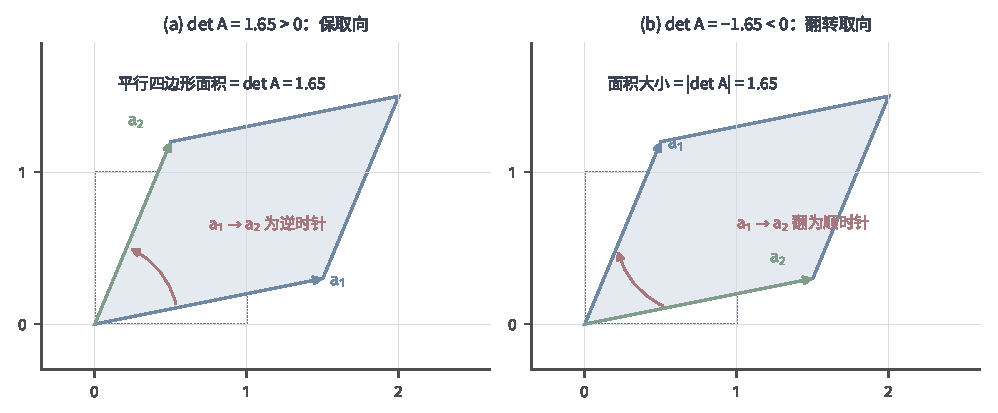
\includegraphics[width=169mm]{figures/01-mathematical-preliminaries-upper/02-linear-spaces/matplotlib/ls-determinant-oriented-volume/ls-determinant-oriented-volume.pdf}
  \caption{行列式作为有向体积的缩放。左：单位正方形由$\bm e_1=(1,0)$、$\bm e_2=(0,1)$张成，面积为$1$。中：$\bm A=\bigl(\begin{smallmatrix}2&0.5\\0&1.5\end{smallmatrix}\bigr)$把它映成由$\bm A\bm e_1=(2,0)$、$\bm A\bm e_2=(0.5,1.5)$张成的平行四边形，有向面积为$2\cdot1.5-0.5\cdot0=3=\det\bm A>0$（保定向）。右：$\bm A$把$\bm e_1$反射到$(-2,0)$，有向面积为$-3$（反定向）。向量与数值均为解析教学例。}
  \label{fig:ls-determinant-oriented-volume}
\end{figure*}

为了直接由矩阵元素计算，把$\bm A\bm e_j=\sum_i a_{i,j}\bm e_i$代入楔积展开，得到有限和
\[
 \det\bm A
 =\sum_{\pi\in S_d}\operatorname{sgn}(\pi)
   \prod_{i=1}^d a_{i,\pi(i)}.
\]
这里$S_d$是$\{1,\ldots,d\}$到自身的全部双射，每个$\pi$规定第$i$行选取第$\pi(i)$列。$d=2$时两种列次序的逆序对数分别为$0$与$1$，正好得到$ad-bc$。行列式因而是矩阵元素的多项式。例如$\begin{pmatrix}1&2\\3&4\end{pmatrix}$的行列式为$-2$，与它的迹$5$是两个不同的量。

由楔积的规则可逐条读出行列式的列变换性质：对每一列分别线性；交换两列变号，两列相同则为零；把某列的倍数加到另一列上不改变行列式。把排列展开中的$\pi$换成逆排列，得到$\det(\bm A^\top)=\det\bm A$，所以这些规则对行同样成立。三角矩阵的排列展开中只有主对角线一项非零，故三角行列式等于对角元之积，$\det\bm I_d=1$。行列式不是对整个矩阵线性的函数：$d\geq2$时一般$\det(\bm A+\bm B)\neq\det\bm A+\det\bm B$。

\paragraph{行列式乘法性与可逆判据}

复合两次作用时，体积缩放倍数应当相乘。由楔积的多线性，
\[
 (\bm A\bm B)\bm e_1\wedge\cdots\wedge(\bm A\bm B)\bm e_d
 =(\det\bm B)\,\bm A\bm e_1\wedge\cdots\wedge\bm A\bm e_d
 =(\det\bm A)(\det\bm B)\,\bm e_1\wedge\cdots\wedge\bm e_d,
\]
其中第一步把$\bm B\bm e_j=\sum_i b_{i,j}\bm e_i$代入后，$\bm A$作用在展开式的各项上，系数正是$\det\bm B$。于是
\[
 \det(\bm A\bm B)=\det\bm A\,\det\bm B.
\]
列线性相关时楔积为零，行列式为零；列线性无关时楔积非零，行列式非零。所以方阵可逆恰好等价于行列式非零，且可逆时$\det(\bm A^{-1})=1/\det\bm A$。

在第~\ref{sec:ls-matrix-equivalences}节的相似关系$\bm B=\bm P^{-1}\bm A\bm P$中，由乘法性
\[
 \det\bm B
 =\det(\bm P^{-1})\det\bm A\det\bm P
 =\det\bm A,
\]
相似变换不改变行列式；它与第~\ref{sec:ls-matrix-contractions}节迹的相似不变性一起，是判断两个矩阵能否记录同一映射时可直接计算的两个标量不变量。双线性型在两个输入同时换基时按合同$\bm B=\bm P^\top\bm A\bm P$变换，此时$\det\bm B=(\det\bm P)^2\det\bm A$：合同只保持行列式的符号与非零性，不保持数值。

\paragraph{特征多项式}

行列式把第~\ref{sec:ls-matrix-powers}节的特征值问题化为一个标量方程。$\lambda$是$\bm A$的特征值，当且仅当$(\bm A-\lambda\bm I)\bm v=\bm0$有非零解，即$\bm A-\lambda\bm I$不可逆，也即$\det(\lambda\bm I-\bm A)=0$。定义
\begin{equation}
 p_{\bm A}(z)=\det(z\bm I-\bm A),
 \label{eq:matrix-analysis-characteristic-polynomial}
\end{equation}
称为\term{特征多项式}（characteristic polynomial）。排列展开中只有对角线一项含$z^d$，故它是首项系数为$1$的$d$次实多项式，实特征值恰为它的实根。以$\bm A=\begin{pmatrix}0.8&4\\0&0.5\end{pmatrix}$为例，$p_{\bm A}(z)=(z-0.8)(z-0.5)$，与第~\ref{sec:ls-matrix-powers}节找到的两条特征方向相符；$90^\circ$旋转的特征多项式$z^2+1$没有实根，因而没有实特征向量。相似矩阵的特征多项式相同：$\det(z\bm I-\bm P^{-1}\bm A\bm P)=\det\bigl(\bm P^{-1}(z\bm I-\bm A)\bm P\bigr)=p_{\bm A}(z)$。

根$\lambda$在$p_{\bm A}$中的重数称为\term{代数重数}，特征空间的维数$\dim\ker(\bm A-\lambda\bm I)$称为\term{几何重数}。把$\lambda$的特征空间的一组基（设有$g$个向量）扩充成全空间的基，$\bm A$在新基下成为分块上三角$\begin{pmatrix}\lambda\bm I_g&*\\\bm0&\bm C\end{pmatrix}$，特征多项式含因子$(z-\lambda)^g$，故几何重数不超过代数重数。例如$\begin{pmatrix}0.8&1\\0&0.8\end{pmatrix}$的特征多项式为$(z-0.8)^2$，代数重数为$2$，几何重数却只有$1$。

不同特征值的特征空间之和是直和：若$\sum_\lambda\bm w_\lambda=\bm0$且$\bm w_\lambda$属于相应特征空间，其中非零的$\bm w_\lambda$是不同特征值的特征向量，由第~\ref{sec:ls-matrix-powers}节它们线性无关，所以每个$\bm w_\lambda=\bm0$。因此各特征空间的基合在一起仍线性无关。由此得到可对角化的判据：$\bm A$实可对角化，当且仅当$p_{\bm A}$能分解为实一次因子之积，且每个特征值的几何重数等于代数重数。充分性是因为此时几何重数之和等于$d$，各特征空间的基合成一组特征基；必要性是因为$\bm A=\bm V\bm\Lambda\bm V^{-1}$时$p_{\bm A}(z)=\prod_i(z-\lambda_i)$，$\lambda$在$\bm\Lambda$对角线上出现的次数既是代数重数，也是$\bm\Lambda-\lambda\bm I$的零空间维数，而相似变换不改变零空间维数。

\paragraph{余子式与古典伴随恒等式}

行列式还可以按一行展开。对$d\geq2$，删除第$i$行、第$j$列得到的$(d-1)$阶子矩阵记为$\bm A^{(i,j)}$，定义\term{代数余子式}（cofactor）
\[
 C_{i,j}=(-1)^{i+j}\det\bm A^{(i,j)}.
\]
把排列展开按第$i$行选取的列分类，得到$\det\bm A=\sum_{j=1}^d a_{i,j}C_{i,j}$；按列同样有$\det\bm A=\sum_{i=1}^d a_{i,j}C_{i,j}$。把全部代数余子式排成矩阵$\bm C$，其转置称为\term{古典伴随}（classical adjugate）$\operatorname{adj}(\bm A)=\bm C^\top$。

\begin{theorem}[古典伴随恒等式]
\label{thm:ls-adjugate-identity}
对任意$d$阶方阵$\bm A$，
\[
 \bm A\,\operatorname{adj}(\bm A)
 =\operatorname{adj}(\bm A)\,\bm A
 =(\det\bm A)\,\bm I_d.
\]
\end{theorem}
\begin{proof}
乘积$\bm A\bm C^\top$的$(i,k)$元素为$\sum_j a_{i,j}C_{k,j}$。当$i=k$时，这正是沿第$i$行展开的$\det\bm A$；当$i\neq k$时，它是把第$k$行换成第$i$行后的矩阵沿第$k$行的展开，新矩阵有两行相同，行列式为零。于是$\bm A\bm C^\top=(\det\bm A)\bm I_d$。按列展开同样得到$\bm C^\top\bm A=(\det\bm A)\bm I_d$。
\end{proof}

古典伴随是由余子式得到的代数构造，与第~\ref{sec:ls-adjoints}节由内积配对定义的伴随不是同一个对象。$\det\bm A\neq0$时，恒等式给出逆的代数表达$\bm A^{-1}=\operatorname{adj}(\bm A)/\det\bm A$，二阶时即$\begin{pmatrix}a&b\\c&d\end{pmatrix}^{-1}=\frac1{ad-bc}\begin{pmatrix}d&-b\\-c&a\end{pmatrix}$。高阶时展开余子式的代价是阶乘级的，恒等式主要作为证明工具，例如第~\ref{sec:ls-matrix-power-behavior}节的Cayley--Hamilton定理。

\section{张量运算}
\label{sec:ls-tensor-operations}

前面的运算大多把同类对象合成同类对象。张量运算处理多个槽位：张量积把多个输入的槽位全部保留下来，组合成一个带更多轴的对象；Kronecker积是两个矩阵的张量积在坐标下的分块记录；缩约则反过来，指定一对槽位对齐求和，把多轴对象汇总成更低阶的对象。三者共同组成多轴数据的基本运算，内积、矩阵乘法与迹都是其中的特例。

\subsection{张量积}
\label{sec:ls-tensor-products}
\label{sec:linear-algebra-joint-operations}

\subsubsection{定义与含义}

\paragraph{张量积与简单张量}

设$\bm x\in\mathbb R^m$、$\bm y\in\mathbb R^n$，它们的\term{张量积}（tensor product）$\bm x\otimes\bm y$是一个$m\times n$数组，元素为$(\bm x\otimes\bm y)_{i,j}=x_i y_j$。这样的对象称为\term{简单张量}（simple tensor）。例如$\bm x=(1,2)^\top$、$\bm y=(3,-1)^\top$给出$\bm x\otimes\bm y=\begin{pmatrix}3&-1\\6&-2\end{pmatrix}$，每一行都是$\bm y$的倍数，每一列都是$\bm x$的倍数。一般张量是若干简单张量之和$\sum_s\bm x_s\otimes\bm y_s$；并非每个二阶张量都能写成单个简单张量，正如并非每个矩阵都是秩一矩阵。图~\ref{fig:ls-tensor-product-slots} 展示张量积怎样保留两个因子的槽位。
\begin{figure}[htbp]
  \centering
  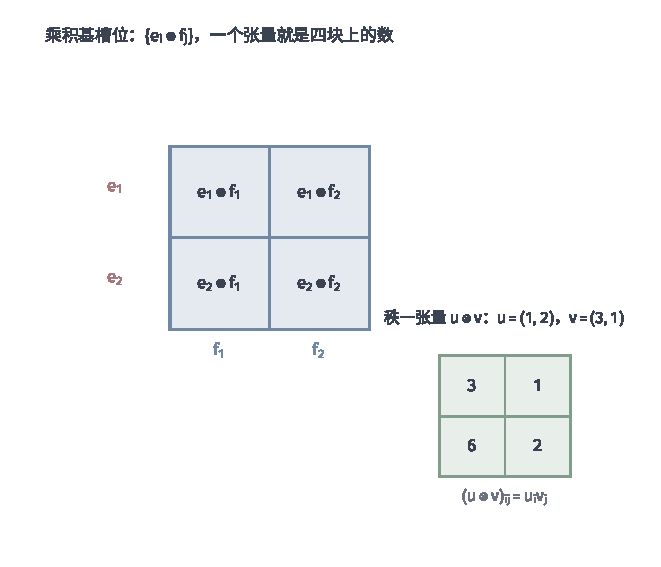
\includegraphics[width=112mm]{figures/01-mathematical-preliminaries-upper/02-linear-spaces/matplotlib/ls-tensor-product-slots/ls-tensor-product-slots.pdf}
  \caption{张量积并排保留两个因子的槽位。左：$\bm u\in\mathbb R^2$、$\bm v\in\mathbb R^3$。右：$\bm u\otimes\bm v$排成$2\times3$网格，每行由$\bm v$方向复制并按$u_i$缩放；它是秩一张量，数值由$\bm u=(1,0.6)$、$\bm v=(1,0.5,0.2)$直接相乘得到，是教学构造。}
  \label{fig:ls-tensor-product-slots}
\end{figure}

取$\mathbb R^m$的基$\bm e_i$与$\mathbb R^n$的基$\bm f_j$，产品基$\bm e_i\otimes\bm f_j$共$mn$个，构成张量积空间的一组基，故维数为$mn$。三个向量的张量积$(\bm x\otimes\bm y\otimes\bm z)_{i,j,k}=x_i y_j z_k$保留三条轴，多重张量积按同样规则逐槽位相乘。

张量积的作用是把双线性映射变成线性映射。给定双线性映射$B:\mathbb R^m\times\mathbb R^n\to W$，存在唯一的线性映射$\widetilde B:\mathbb R^m\otimes\mathbb R^n\to W$使$\widetilde B(\bm x\otimes\bm y)=B(\bm x,\bm y)$：先在产品基上规定$\widetilde B(\bm e_i\otimes\bm f_j)=B(\bm e_i,\bm f_j)$，再线性延拓即可。以欧氏内积$B(\bm x,\bm y)=\bm x^\top\bm y$为例，提升后的线性映射把$\bm x\otimes\bm y$送到$\sum_ix_iy_i$，也就是对数组$\bm x\otimes\bm y$的对角线求和——这正是后面的缩约。

二阶张量与矩阵是同一组数的两种记录：张量强调槽位来自哪一组输入，矩阵强调行列在复合中的角色。二者由第~\ref{sec:ls-reshaping}节的重排互相转换，数值不变。

\subsubsection{运算性质}

张量积对两个因子分别线性：$(a\bm x)\otimes\bm y=\bm x\otimes(a\bm y)=a(\bm x\otimes\bm y)$，且对加法分配；括号可以在槽位间移动，$(\bm x\otimes\bm y)\otimes\bm z=\bm x\otimes(\bm y\otimes\bm z)$。交换两个槽位对应轴置换：$\bm x\otimes\bm y$的$(i,j)$元素$x_iy_j$是$\bm y\otimes\bm x$的$(j,i)$元素，两者互为转置。

第~\ref{sec:ls-exterior-determinants}节的楔积可以由张量积经反对称化得到：$\bm x\wedge\bm y$对应$\bm x\otimes\bm y-\bm y\otimes\bm x$。这里只指出联系，楔积的构造不依赖张量积。

在Frobenius内积下，简单张量的配对与范数都分离：
\[
 \langle\bm x\otimes\bm y,\bm x'\otimes\bm y'\rangle_{\mathrm F}
 =\langle\bm x,\bm x'\rangle\langle\bm y,\bm y'\rangle,
 \qquad
 \lVert\bm x\otimes\bm y\rVert_{\mathrm F}=\lVert\bm x\rVert\,\lVert\bm y\rVert,
\]
因为$\sum_{i,j}x_iy_jx'_iy'_j=(\sum_ix_ix'_i)(\sum_jy_jy'_j)$。以$\bm x=(1,2)^\top$、$\bm y=(3,-1)^\top$为例，乘积范数为$\sqrt5\cdot\sqrt{10}=5\sqrt2$，与直接对$\begin{pmatrix}3&-1\\6&-2\end{pmatrix}$求Frobenius范数一致。

\paragraph{Schur乘积定理}

配对的分离性给出一个关于逐项乘积的结论。设$\bm A,\bm B$均为半正定矩阵，由定理~\ref{thm:ls-gram-factor}，它们各有Gram因子$\bm A=\bm U^\top\bm U$、$\bm B=\bm V^\top\bm V$，即$A_{i,k}=\langle\bm u_i,\bm u_k\rangle$、$B_{i,k}=\langle\bm v_i,\bm v_k\rangle$，其中$\bm u_i,\bm v_i$是两个因子的列。考虑向量组$\{\bm u_i\otimes\bm v_i\}$，其Gram矩阵为
\[
 \langle\bm u_i\otimes\bm v_i,\bm u_k\otimes\bm v_k\rangle_{\mathrm F}
 =\langle\bm u_i,\bm u_k\rangle\langle\bm v_i,\bm v_k\rangle
 =A_{i,k}B_{i,k}.
\]
Gram矩阵恒半正定，故逐项乘积$\bm A\odot\bm B$半正定，这就是\term{Schur乘积}定理。例如$\bm A=\bm B=\begin{pmatrix}1&1\\1&2\end{pmatrix}$，逐项乘积$\begin{pmatrix}1&1\\1&4\end{pmatrix}$的行列式为$3>0$、对角元为正，仍半正定。核方法中两个核矩阵的逐项乘积仍是合法核矩阵，依据就是这一定理。

\subsection{Kronecker积}
\label{sec:ls-kronecker-products}

当两个因子本身都是矩阵时，张量积空间上的联合作用可以写成一张分块矩阵，这就是Kronecker积。

\subsubsection{定义与含义}

\paragraph{Kronecker积的定义}

对$\bm A\in\mathbb R^{m\times n}$、$\bm B\in\mathbb R^{p\times q}$，定义
\begin{equation}
 \bm A\otimes\bm B
 =\begin{bmatrix}
  A_{1,1}\bm B&\cdots&A_{1,n}\bm B\\
  \vdots&\ddots&\vdots\\
  A_{m,1}\bm B&\cdots&A_{m,n}\bm B
 \end{bmatrix}\in\mathbb R^{mp\times nq}.
 \label{eq:linear-algebra-kronecker-product}
\end{equation}
每个块$A_{i,j}\bm B$是$\bm B$整体乘以$A_{i,j}$。图~\ref{fig:ls-kronecker-block-structure} 展示这种逐元素替换的分块结构。
\begin{figure}[htbp]
  \centering
  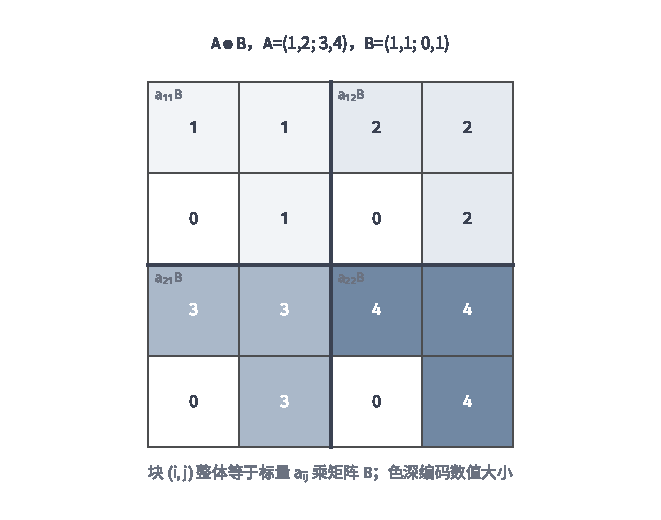
\includegraphics[width=112mm]{figures/01-mathematical-preliminaries-upper/02-linear-spaces/matplotlib/ls-kronecker-block-structure/ls-kronecker-block-structure.pdf}
  \caption{Kronecker积的分块结构。上：$\bm A=\bigl(\begin{smallmatrix}1&2\\3&4\end{smallmatrix}\bigr)$、$\bm B=\bigl(\begin{smallmatrix}10&20\\30&40\end{smallmatrix}\bigr)$。下：$\bm A\otimes\bm B$是把$\bm A$的每个元素替换为该元素乘$\bm B$得到的$4\times4$分块矩阵，块边界用白线强调。数值由定义直接计算，是教学例。}
  \label{fig:ls-kronecker-block-structure}
\end{figure}

在产品基$\bm e_i\otimes\bm f_j$下，$(\bm A\otimes\bm B)(\bm x\otimes\bm y)=(\bm A\bm x)\otimes(\bm B\bm y)$：第一个槽位只经过$\bm A$，第二个槽位只经过$\bm B$，两个作用并行而不串联。这与矩阵乘法把前后两次作用串成一条链形成对照。向量的张量积是它的特例：两个列向量的Kronecker积就是按行展开的$\bm x\otimes\bm y$。

\subsubsection{运算性质}

按成对索引分别求和，相容乘积满足混合乘积规则
\begin{equation}
 (\bm A\otimes\bm B)(\bm C\otimes\bm D)
 =(\bm A\bm C)\otimes(\bm B\bm D),
 \label{eq:matrix-analysis-kronecker-mixed-product}
\end{equation}
其中$\bm A\bm C$与$\bm B\bm D$分别相容：左侧的块$(i,k)$为$\sum_jA_{i,j}C_{j,k}\bm B\bm D$，恰是右侧的块。由此得到$(\bm A\otimes\bm B)^\top=\bm A^\top\otimes\bm B^\top$；两因子都可逆时$(\bm A\otimes\bm B)^{-1}=\bm A^{-1}\otimes\bm B^{-1}$；方阵情形下$\operatorname{tr}(\bm A\otimes\bm B)=\operatorname{tr}\bm A\operatorname{tr}\bm B$。

结合第~\ref{sec:ls-reshaping}节的向量化，对$\bm A\in\mathbb R^{p\times m}$、$\bm X\in\mathbb R^{m\times n}$、$\bm B\in\mathbb R^{n\times q}$，
\begin{equation}
 \operatorname{vec}(\bm A\bm X\bm B)
 =(\bm B^\top\otimes\bm A)\operatorname{vec}(\bm X).
 \label{eq:matrix-analysis-vec-kronecker}
\end{equation}
证明只需比较输出元素：两侧的$(i,j)$元素均为$\sum_{\ell=1}^m\sum_{k=1}^n A_{i,\ell}X_{\ell,k}B_{k,j}$。固定$\bm A,\bm B$后这是关于$\bm X$的线性映射，把两侧同时作用于未知矩阵的方程化成普通线性方程组。

表~\ref{tab:linear-algebra-products-and-shapes}汇总本章几种“乘法”的形状条件与索引作用。

\begin{table*}[htbp]
 \centering\small
 \begin{tabularx}{\linewidth}{@{}lXX@{}}
  \toprule
  运算 & 形状条件与输出 & 索引作用\\
  \midrule
  $\bm A\bm B$ & $(m\times n)(n\times p)\to m\times p$ & 汇总共同索引\\
  $\bm A\odot\bm B$ & 同为$m\times n$，输出仍为$m\times n$ & 同位置相乘，不求和\\
  $\bm A\otimes\bm B$ & $(m\times n)$与$(p\times q)\to(mp)\times(nq)$ & 保留两组成对索引\\
  $\langle\bm x,\bm y\rangle$ & 两个$n$维向量，输出标量 & 配对后汇总\\
  \bottomrule
 \end{tabularx}
 \caption{相乘符号对应不同操作。先检查消去哪些索引，再判断其线性性和输出含义。}
 \label{tab:linear-algebra-products-and-shapes}
\end{table*}

\subsection{张量缩约}
\label{sec:ls-tensor-contraction}

张量积把槽位全部保留，缩约则指定一对相容槽位，对齐相乘后求和，消去这对轴。

\subsubsection{定义与性质}

\paragraph{张量缩约的定义}

缩约须先指定参与求和的轴，并保证对应尺寸相同。例如$\bm A\in\mathbb R^{m\times d\times r}$、$\bm B\in\mathbb R^{d\times n\times r}$可定义
\[
 c_{i,j}=\sum_{k=1}^d\sum_{s=1}^r a_{i,k,s}b_{k,j,s},
\]
同时消去$k$与$s$两对轴。被求和的轴消失，其余轴保留：上例输出为$m\times n$矩阵。矩阵乘法是只消去一对轴的特例，内积是两个向量唯一一对轴的缩约。对$\bm X\in\mathbb R^{b\times\ell\times d}$的最后一轴作用$\bm W\in\mathbb R^{d\times h}$，$z_{i,j,r}=\sum_k x_{i,j,k}w_{k,r}$，输出形状为$b\times\ell\times h$。写出索引就能检查哪些轴被消去、哪些轴应当保留。图~\ref{fig:ls-tensor-contraction} 沿一对选中的轴求和并保留其余轴。
\begin{figure}[htbp]
  \centering
  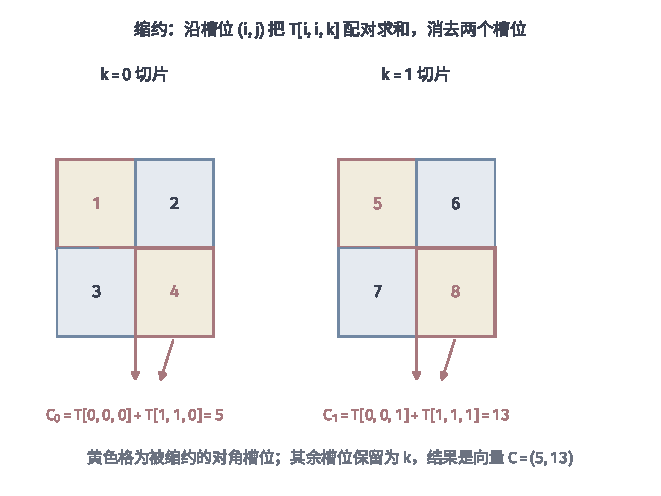
\includegraphics[width=112mm]{figures/01-mathematical-preliminaries-upper/02-linear-spaces/matplotlib/ls-tensor-contraction/ls-tensor-contraction.pdf}
  \caption{张量缩约沿选中的一对轴求和、保留其余轴。左：二阶张量按行和列着色；选中列轴（虚线箭头）沿列求和，输出对每行汇总为一个值。右：缩约后得到$3$个输出，分别对应原矩阵三行的行和，颜色由红(小)经黄到蓝(大)。张量与数值均为解析教学例。}
  \label{fig:ls-tensor-contraction}
\end{figure}

系数是简单张量时，缩约可以分开计算。一次读取同时依赖三组向量$\bm x\in\mathbb R^m$、$\bm y\in\mathbb R^n$、$\bm z\in\mathbb R^p$时，若系数数组是秩一张量$\bm a\otimes\bm b\otimes\bm c$，则
\begin{equation}
 \left\langle\bm a\otimes\bm b\otimes\bm c,
 \bm x\otimes\bm y\otimes\bm z\right\rangle_{\mathrm F}
 =(\bm a^\top\bm x)(\bm b^\top\bm y)(\bm c^\top\bm z),
 \label{eq:linear-algebra-rank-one-contraction}
\end{equation}
三重求和分离成三个内积的乘积。例如取$\bm a=(1,2)^\top$、$\bm b=(3,-1)^\top$、$\bm c=(2,1)^\top$，$\bm x=(2,1)^\top$、$\bm y=(1,1)^\top$、$\bm z=(1,-1)^\top$，三个内积依次为$4,2,1$，读取等于$8$。

固定配对对象后，缩约对被作用张量线性。多对轴的缩约是有限和，求和次序可以交换，结果与先消哪一对轴无关。$\operatorname{softmax}$、逐元素非线性等操作不属于缩约：一个模型即使由缩约和这些操作交替组成，固定系数时的线性也不代表整体线性。

\subsubsection{矩阵上的缩约}
\label{sec:ls-matrix-contractions}
\label{sec:prelim-matrix-trace}

\paragraph{迹的定义}

方阵最自然的缩约是把行轴与列轴对齐到同一索引后求和。对$n$阶方阵，定义\term{迹}（trace）
\[
 \operatorname{tr}(\bm A)=\sum_{i=1}^n A_{i,i}.
\]
例如$\bm A=\begin{pmatrix}1&2\\3&4\end{pmatrix}$的迹为$1+4=5$。迹是对角元之和，不是全部元素之和。有限和的线性规则直接给出$\operatorname{tr}(a\bm A+b\bm B)=a\operatorname{tr}(\bm A)+b\operatorname{tr}(\bm B)$。

矩阵乘法没有交换律，但乘积的迹在合法的循环移位下不变。对$\bm A\in\mathbb R^{m\times n}$、$\bm B\in\mathbb R^{n\times m}$，有限和换序给出
\begin{equation}
 \operatorname{tr}(\bm A\bm B)
 =\sum_{i=1}^m\sum_{j=1}^n A_{i,j}B_{j,i}
 =\operatorname{tr}(\bm B\bm A).
 \label{eq:linear-algebra-trace-cyclic}
\end{equation}
两个乘积甚至可以是不同阶的方阵；相等的是迹，不是矩阵本身。三因子只能循环移动，$\operatorname{tr}(\bm A\bm B\bm C)=\operatorname{tr}(\bm B\bm C\bm A)=\operatorname{tr}(\bm C\bm A\bm B)$，不能任意交换相邻因子：取$\bm A=\begin{pmatrix}1&0\\0&0\end{pmatrix}$、$\bm B=\begin{pmatrix}0&0\\1&0\end{pmatrix}$、$\bm C=\begin{pmatrix}0&1\\0&0\end{pmatrix}$，则$\bm A\bm B\bm C=\bm0$，而$\bm A\bm C\bm B=\begin{pmatrix}1&0\\0&0\end{pmatrix}$，迹分别为$0$与$1$。由循环性，相似变换不改变迹：
\[
 \operatorname{tr}(\bm P^{-1}\bm A\bm P)
 =\operatorname{tr}(\bm A\bm P\bm P^{-1})
 =\operatorname{tr}\bm A.
\]
迹与行列式一样，是第~\ref{sec:ls-matrix-equivalences}节相似关系下的标量不变量。

第~\ref{sec:ls-inner-products}节定义的Frobenius内积把对应位置相乘后相加，写成缩约就是
\[
 \langle\bm A,\bm B\rangle_{\mathrm F}
 =\sum_{i,j}A_{i,j}B_{i,j}
 =\operatorname{tr}(\bm A^\top\bm B),
\]
因为$\bm A^\top\bm B$第$j$个对角元为$\sum_i A_{i,j}B_{i,j}$，再对$j$求和恰好遍历所有位置。计算$\operatorname{tr}(\bm A\bm B)$时也不必形成乘积：只需$\sum_{i,j}A_{i,j}B_{j,i}$，代价为$mn$而非$m^2n$。

\section{本章小结}
\label{sec:ls-operations-summary}

本章回答第~\ref{chap:linear-representation}章记录下来的对象怎样运算。对每种运算，我们都规定了输入的相容条件与输出形状，说明了它的运算逻辑，并给出可以直接使用的性质。

第一组运算把对象合并成同类对象。加法与数乘要求形状一致，线性组合把多个记录合成一个，映射的叠加对应矩阵的逐项相加。“乘法”有两种含义：逐项乘法在同一位置相乘、不汇总任何索引，依赖坐标；矩阵乘法来自映射复合，汇总共同索引，满足结合律而不满足交换律。分块后块可以像数一样相乘。同一方阵的反复作用得到矩阵幂；特征方向是幂在其上只作标量缩放的方向，可对角化时幂化为对角元的乘方。转置、轴置换、reshape与向量化只改变记录位置，不改变数值，但会改变秩与诱导范数这类依赖排列的量。

第二组运算给对象以几何。内积把两个对象配成标量，由Cauchy--Schwarz不等式得到夹角；加权内积由正定矩阵给出，Gram因子定理说明它只是换了一组欧氏坐标；Gram矩阵记录一组向量的全部配对，非奇异当且仅当它们线性无关，由此得到正交直和。范数给出误差的大小：$\ell_p$范数由Hölder不等式联系，诱导矩阵范数度量最坏放大并满足次乘性，对偶范数回答线性读取在误差预算下的最大变化。伴随把内积配对中的作用从输出端搬到输入端，标准内积下就是转置，加权内积下要带上两侧权重。

第三组运算处理多个槽位。外积用交替多线性记录有向体积，最高维系数就是行列式：它满足乘法性，非零当且仅当矩阵可逆，并把特征值问题化为特征多项式的求根；几何重数与代数重数是否相等决定能否对角化。张量积保留全部槽位，Kronecker积是矩阵张量积的分块记录，混合乘积规则与向量化恒等式把两者与普通矩阵乘法联系起来；缩约沿指定槽位求和，矩阵乘法、内积与迹都是它的实例。

这些运算都在精确输入、一次计算的前提下讨论。点到子空间的最近点、方程的求解与逼近在第~\ref{chap:linear-equations-and-optimization}章展开，有限维范数之间的比较也在那里随距离问题建立；矩阵指数等矩阵函数、输入误差的放大与反复作用的长期行为留给第~\ref{chap:linear-analysis}章。


\chapter{方程和优化}
\label{chap:linear-equations-and-optimization}
\label{sec:linear-algebra-reachability-solvability}

正向作用给定输入就能算出输出；反向问题则固定矩阵和目标，寻找使输出符合要求的输入。
前面各章建立了向量、矩阵、内积、范数与线性映射的表示，本章把这些表示放进四类具体任务：
第一类是\term{精确解}（exact solution），要求等式$\bm A\bm x=\bm b$严格成立，
先判断目标是否可达、解是否唯一，再用直接法或迭代法把解求出来；
第二类是\term{残差最小}（least-squares fit），目标不可达时不要求等式成立，
转而最小化输出与目标的差距；第三类是\term{结构逼近}（structured approximation），
在秩、正交性、对称性或谱范围等限制下寻找离目标最近的矩阵；
第四类是\term{矩阵方程}（matrix equation），未知量本身是矩阵，
单侧、双侧或多项作用同时约束它。子空间最近点一节先解决目标到子空间的距离问题，
它为精确解的选解和残差最小提供共同的正交几何。

每类任务都按相同顺序回答三个问题：满足条件的对象是否存在、是否唯一；
用什么构造把它算出来；算完以后怎样核验。本章只说明方法能否执行、每一步怎样更新、
以及用什么残差或条件核对结果；迭代序列收敛得多快、数据扰动会放大多少误差，
分别由后续收敛分析与扰动分析章节承担，这里不提前证明速度与敏感度。

% 6.1 子空间最近点；6.2 线性方程：精确求解

\section{子空间最近点}
\label{sec:ls-subspace-nearest-points}
\label{sec:linear-algebra-decomposition-projection}

\subsection{问题与条件}

设$V$为有限维实内积空间，$U\subseteq V$为子空间，给定目标$\bm y\in V$。
\term{子空间最近点}问题要求在$U$中找到使距离$\lVert\bm y-\bm p\rVert$最小的点
$\bm p\in U$。典型场景是：可达输出全部落在列空间$U=\operatorname{range}(\bm B)$中，
目标$\bm y$未必落在其中，于是在可达输出里挑离它最近的一个；相容方程选解时，
又要在同一仿射解集里挑范数最小的代表，二者都是同一个正交几何问题。
距离由当前内积诱导，更换内积就更换“最近”的几何：
斜坐标系里沿坐标轴拆分得到的两个分量并不垂直，丢掉一个方向后剩下的点一般不是最近点。
前面的内积与正交关系已经建立，本节不再重复定义。我们先在一般范数下说明最近点存在，
这需要有限维的紧性与范数等价；再用已有的正交分量证明内积下的唯一性，最后解决一般基下
怎样把最近点算出来。

取$U$的一组基$\bm b_1,\ldots,\bm b_r$，写成矩阵$\bm B=[\bm b_1\;\cdots\;\bm b_r]$，
则$U=\{\bm B\bm c:\bm c\in\mathbb R^r\}$，最近点问题化为
\begin{equation}
 \min_{\bm c\in\mathbb R^r}\lVert\bm y-\bm B\bm c\rVert_2.
 \label{eq:ls-nearest-point-coefficients}
\end{equation}
换一组基只更换系数$\bm c$的坐标，不改变点集$U$，因而不改变最近点本身。
困难在于：基向量一般互不正交，系数不能逐个由内积直接读出，
逐个扣除又会互相串扰，需要先把基整理成便于计算的形式。
例如在$\mathbb R^2$中取$U=\operatorname{span}\{(1,1)^\top,(1,0)^\top\}$，
两个基方向夹$45^\circ$，目标$(0,1)^\top$的系数不能直接由内积读取，
先正交化才能得到唯一系数。

\subsection{距离与误差尺度}
\label{sec:ls-error-scale-comparison}

最近点问题的目标值是点到子空间的距离。对一般范数$\lVert\cdot\rVert$与子空间$U$，定义
\[
 d(\bm y,U)=\inf_{\bm u\in U}\lVert\bm y-\bm u\rVert.
\]
定义只给出下确界。要说明某个$\bm u\in U$真的达到它，需要两件此前没有建立的工具：有限维闭有界集上连续函数取到最小值，以及更换范数不改变“闭”“有界”“收敛”这些定性结论。本小节先建立这两件工具，再看一般范数下最近点存在但未必唯一；内积范数下的唯一性与计算在后面几小节完成。

第~\ref{chap:function-limits}章的Bolzano--Weierstrass定理~\ref{thm:analysis-bounded-subsequence} 保证有界实数列有收敛子列。对$\mathbb R^d$中的有界向量序列$\bm x_n$，先对第一坐标抽取收敛子列，再在该子列上对第二坐标抽取，逐坐标重复$d$次；最后得到的子列每个坐标都收敛，因而向量收敛。若序列取自闭集，闭集的序列判据（引理~\ref{lem:analysis-closed-sequence-criterion}）保证极限仍留在集合内。

\paragraph{有限维闭有界集上的极值定理}

\begin{theorem}[有限维闭有界集上的极值定理]
\label{thm:ls-extreme-value}
设$K\subseteq\mathbb R^d$非空、闭且有界，$f:K\to\mathbb R$连续，则$f$有界，并在$K$上达到最小值与最大值。
\end{theorem}
\begin{proof}
若$f$无界，可选$\bm x_n\in K$使$|f(\bm x_n)|>n$；有界序列取收敛子列$\bm x_{n_k}\to\bm x\in K$，连续性给出$f(\bm x_{n_k})\to f(\bm x)$，与$|f(\bm x_{n_k})|>n_k$矛盾。令$m=\inf_K f$，对每个$n$选$\bm x_n\in K$使$m\leq f(\bm x_n)<m+1/n$，再取收敛子列$\bm x_{n_k}\to\bm x^\star\in K$，得$f(\bm x^\star)=m$。对$-f$重复论证即得最大值。
\end{proof}
证明只使用逐坐标子列与闭性，不依赖范数等价。这里的“闭”“有界”按坐标理解；下面的范数等价说明换成任意范数，这两个概念不变。

\paragraph{有限维范数等价}

固定基$(\bm b_1,\ldots,\bm b_d)$，记坐标最大范数$\lVert\bm x\rVert_c=\max_j|x_j|$。对任意范数$p$，三角不等式给出
\[
 p\Bigl(\sum_jx_j\bm b_j\Bigr)\leq\sum_j|x_j|p(\bm b_j)\leq C\lVert\bm x\rVert_c,
 \qquad C=\sum_jp(\bm b_j).
\]
反向三角不等式$|p(\bm x)-p(\bm y)|\leq p(\bm x-\bm y)\leq C\lVert\bm x-\bm y\rVert_c$说明$p$对坐标连续。坐标单位球面$\lVert\bm x\rVert_c=1$是闭有界集，连续的$p$在其上取到最小值$m$；正定性使$m>0$。缩放任意非零$\bm x$得到
\begin{equation}
 m\lVert\bm x\rVert_c\leq p(\bm x)\leq C\lVert\bm x\rVert_c.
 \label{eq:linear-algebra-finite-norm-equivalence}
\end{equation}
\begin{theorem}[有限维范数等价]
\label{thm:ls-norm-equivalence}
有限维实向量空间上任意两个范数$p,q$都等价：存在常数$c,C>0$使$c\,q(\bm x)\leq p(\bm x)\leq C\,q(\bm x)$对所有$\bm x$成立。
\end{theorem}
\begin{proof}
分别由$p\leq C_p\lVert\cdot\rVert_c$、$q\geq m_q\lVert\cdot\rVert_c$得$p\leq(C_p/m_q)q$，交换$p,q$得反向下界。
\end{proof}
证明顺序是先坐标子列、再极值、后等价，没有用范数等价证明自身。常数依赖空间、基与所选范数，不能忽略维数：第~\ref{sec:ls-norms-distances}节$\ell_1$与$\ell_2$之间的界含$\sqrt d$，$d$增大时同一误差在不同尺度下的读数可以相差很多。范数等价保证坐标收敛与任意范数收敛相互推出，也保证诱导矩阵范数与对偶范数定义中的上确界有限并且可以达到：它们都是连续函数在某个范数单位球（闭有界集）上的最大值。

\paragraph{子空间闭性与商范数}
\label{sec:ls-quotient-norms}

点到子空间的距离为零，是否意味着点就在子空间里？这取决于子空间是否闭。
\begin{theorem}[有限维子空间闭性]
\label{thm:ls-subspace-closed}
有限维赋范空间的每个线性子空间$U$都是闭集：若$\bm x_n\in U$且$\bm x_n\to\bm x$，则$\bm x\in U$。
\end{theorem}
\begin{proof}
取$U$的基扩充为整个空间的基，$\bm x_n$在补充方向上的坐标恒为零。范数等价保证坐标是连续函数，极限$\bm x$在补充方向上的坐标是零序列的极限，故为零，于是$\bm x\in U$。
\end{proof}
于是$d(\bm x,U)=0$当且仅当$\bm x\in U$：取$\bm u_n\in U$使$\lVert\bm x-\bm u_n\rVert\to0$，闭性给出$\bm x\in U$。第~\ref{sec:ls-quotient-spaces}节的商空间$V/U$由等价类$[\bm x]=\bm x+U$组成，同一类中各代表元到$U$的距离相同，因此可以定义商范数
\[
 \lVert[\bm x]\rVert_{V/U}=d(\bm x,U)=\inf_{\bm u\in U}\lVert\bm x-\bm u\rVert.
\]
齐次性与三角不等式由原范数继承，正定性正是上面的闭性结论；若$U$不闭，只能得到半范数。

\paragraph{一般范数下的最近点}

现在可以回答最近点是否存在。取$\bm u=\bm0$可知$d(\bm y,U)\leq\lVert\bm y\rVert$；而$\lVert\bm u\rVert>2\lVert\bm y\rVert$时$\lVert\bm y-\bm u\rVert\geq\lVert\bm u\rVert-\lVert\bm y\rVert>\lVert\bm y\rVert$，这样的$\bm u$不可能更近。所以只需在$K=\{\bm u\in U:\lVert\bm u\rVert\leq2\lVert\bm y\rVert\}$上求最小值。由子空间闭性与范数等价，$K$在坐标意义下闭且有界，连续函数$\bm u\mapsto\lVert\bm y-\bm u\rVert$在其上取到最小值。因此在任意范数下，有限维子空间中都存在最近点。

唯一性却可能失败。取$\ell_\infty$范数、$U=\operatorname{span}\{(1,0)^\top\}$、$\bm y=(0,1)^\top$，则$\lVert\bm y-(t,0)^\top\rVert_\infty=\max\{|t|,1\}$，所有$|t|\leq1$的点都达到最小距离$1$。单位球的边界含有线段时就会出现这种情形。内积范数下的情形不同，下面用勾股恒等式证明最近点唯一，并且可以由线性方程算出。

\subsection{存在性与唯一性}

由\ref{sec:ls-orthogonality}建立的有限维内积空间关于子空间的正交直和$V=U\oplus U^\perp$，
其中$U^\perp=\{\bm r:\langle\bm u,\bm r\rangle=0,\ \bm u\in U\}$。
于是$\bm y$唯一拆成$\bm y=\bm p+\bm r$，$\bm p\in U$，$\bm r\in U^\perp$。
这个$\bm p$就是待证的最近点。内积范数下不必借助上一小节的极值定理，下面用勾股恒等式直接核验，并同时得到唯一性。

\paragraph{勾股恒等式与最近点判据}

对任意$\bm u\in U$，$\bm p-\bm u\in U$与$\bm r$正交，勾股恒等式给出
\begin{equation}
 \lVert\bm y-\bm u\rVert_2^2
 =\lVert\bm p-\bm u\rVert_2^2+\lVert\bm r\rVert_2^2
 \geq\lVert\bm r\rVert_2^2.
\end{equation}
推导分两步：先写$\bm y-\bm u=(\bm p-\bm u)+\bm r$，其中第一项在$U$内、
第二项在$U^\perp$内，二者正交；正交向量的勾股恒等式把平方范数拆成两项平方和。
第一项非负，故距离平方不小于$\lVert\bm r\rVert_2^2$。等号当且仅当
$\bm p-\bm u=\bm0$，即$\bm u=\bm p$。因此$\bm p$是$U$中唯一的最近点，
最小距离为$\lVert\bm r\rVert_2$，且残差$\bm r=\bm y-\bm p$与$U$中每个向量正交。
这一判据也可反过来使用：若某$\bm p\in U$使$\bm y-\bm p\perp U$，则对任意
$\bm u\in U$，$\bm y-\bm u=(\bm p-\bm u)+(\bm y-\bm p)$正交拆分，
同上得$\lVert\bm y-\bm u\rVert^2=\lVert\bm p-\bm u\rVert^2+\lVert\bm y-\bm p\rVert^2
\geq\lVert\bm y-\bm p\rVert^2$，故它必是唯一最近点。存在性由有限维正交直和
保证，不另调用极值定理；唯一性来自勾股不等式等号条件。

最近点$\bm p$由正交分解唯一确定：勾股不等式的等号只在$\bm u=\bm p$时取得，
不存在另一个$U$中的点达到同样最小距离。在固定基$\bm B$下，由于基向量线性无关，
表示$\bm p=\bm B\bm c$的系数$\bm c$也唯一——若$\bm B\bm c_1=\bm B\bm c_2$，
则$\bm B(\bm c_1-\bm c_2)=\bm0$，线性无关迫使$\bm c_1=\bm c_2$。
要区分两层唯一性：子空间中的点$\bm p$在任意基下都唯一，系数$\bm c$只在无关基下
唯一；基相关时点仍唯一而系数不唯一，第~\ref{sec:ls-exact-linear-equations}节的选解会回到这一区别。
改用正定权重$\bm M$的加权内积
$\langle\bm x,\bm z\rangle_{\bm M}=\bm x^\top\bm M\bm z$时，正交补$U^\perp_{\bm M}$
随之改变，最近点一般不同于标准内积下的点；但$\bm M$正定保证同样的正交直和与
唯一结论成立。例如直线$U=\operatorname{span}\{(1,1)^\top\}$在标准内积下，
点$\bm y=(1,0)^\top$的最近点为$(1/2,1/2)^\top$；若取$\bm M=\operatorname{diag}(1,4)$，
加权正交条件给出$a=1/5$、最近点$(1/5,1/5)^\top$，与标准内积结果不同（完整算例见后文）。
图~\ref{fig:ls-orthogonal-projection-nearest}用一条直线子空间把这一几何固定下来：
连接$\bm y$与最近点$\bm p$的误差垂直于$U$，$U$上任何其他候选点到$\bm y$的距离都更长。

\begin{figure}[htbp]
  \centering
  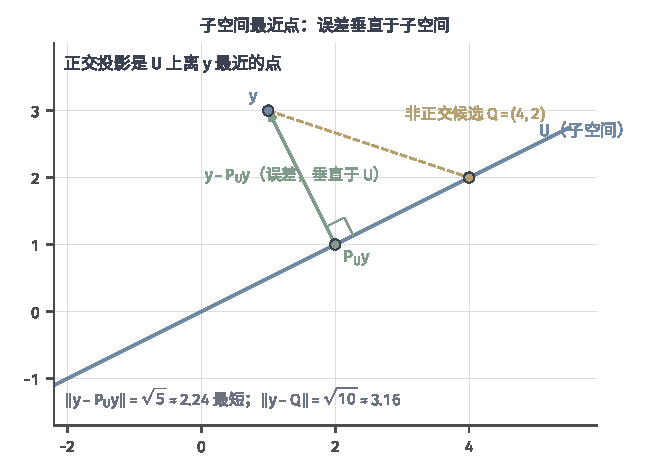
\includegraphics[width=112mm]{figures/01-mathematical-preliminaries-upper/02-linear-spaces/matplotlib/ls-orthogonal-projection-nearest/ls-orthogonal-projection-nearest.pdf}
  \caption{直线子空间$U$（过原点、方向$(2,1)$）上离$\bm y=(1,3)^\top$最近的点是正交投影
  $\bm p=(2,1)^\top$，误差$\bm y-\bm p=(-1,2)^\top$与$U$垂直（直角小方块）；
  同一线上的另一候选$\bm q=(4,2)^\top$到$\bm y$的距离$\sqrt{10}$明显大于最短距离$\sqrt5$。
  这是解析式教学构造。}
  \label{fig:ls-orthogonal-projection-nearest}
\end{figure}

\subsection{求解方法}

\subsubsection{正交化与QR分解}
\label{sec:ls-orthogonalization-qr}

一组向量$\bm q_1,\ldots,\bm q_r$若满足$\langle\bm q_i,\bm q_j\rangle=\delta_{i,j}$，即两两正交且长度为$1$，就称为标准正交组；它的Gram矩阵是单位阵，因而线性无关。张成$U$的标准正交组称为$U$的\term{标准正交基}（orthonormal basis）。
若$U$已有标准正交基$\bm q_1,\ldots,\bm q_r$，系数直接由内积读取：
$\bm p=\sum_j\bm q_j\langle\bm q_j,\bm y\rangle$，每个系数互不干扰。一般基没有这个
便利：基向量夹成斜坐标系，一个方向上的读数混入其他方向，逐个内积不能直接得到
独立系数。所以先把$\bm B$的列整理成正交列与上三角系数的乘积（QR分解），
再读取分量；这一步是把斜坐标换成直角坐标，而不改变点集$U$。

\paragraph{逐方向扣除与Gram--Schmidt}

\term{Gram--Schmidt正交化}按列进行。对$\bm b_j$，先减去它在已有正交方向上的分量：
\begin{equation}
 \bm v_j=\bm b_j-\sum_{i<j}\bm q_i\langle\bm q_i,\bm b_j\rangle,
 \qquad
 \bm q_j=\frac{\bm v_j}{\lVert\bm v_j\rVert_2}.
 \label{eq:ls-classical-gs}
\end{equation}
对$i<j$，$\langle\bm q_i,\bm v_j\rangle
=\langle\bm q_i,\bm b_j\rangle-\langle\bm q_i,\bm b_j\rangle=0$，
故每步$\bm v_j$与先前全部$\bm q_i$正交，归一化后得到新的标准正交方向；
归纳可知$\bm q_1,\ldots,\bm q_j$标准正交且与$\bm b_1,\ldots,\bm b_j$张成同一空间。
例如$\bm b_1=(1,0)^\top$直接给出$\bm q_1=(1,0)^\top$；
$\bm b_2=(1,1)^\top$扣除$\langle\bm q_1,\bm b_2\rangle\bm q_1=(1,0)^\top$后
得$\bm v_2=(0,1)^\top$，归一化即$\bm q_2=(0,1)^\top$。

\paragraph{正交列和上三角系数的形成}

把$\bm b_j=\sum_{i\leq j}r_{i,j}\bm q_i$中的系数$r_{i,j}=\langle\bm q_i,\bm b_j\rangle$
排成上三角矩阵$\bm R$，即得经济型\term{QR分解}
\begin{equation}
 \bm B=\bm Q\bm R,\qquad
 \bm Q^\top\bm Q=\bm I_r,\quad\bm R\text{ 上三角且对角元为正}.
 \label{eq:ls-qr-factorization}
\end{equation}
$\bm Q\in\mathbb R^{m\times r}$的列张成$U$，$\bm R$记录每列相对正交方向的组合系数。
图~\ref{fig:vol1-add-linear-qr-columns}给出最小的二维情形：保留第一条单位方向，
再从第二列减去它在第一方向上的分量，列空间不变，减去的部分记进$\bm R$。
\begin{figure}[!htb]
  \centering
  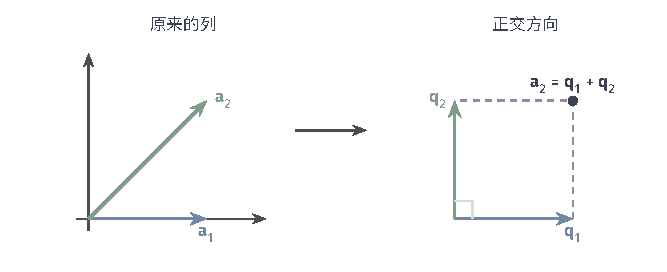
\includegraphics[width=112mm]{figures/01-mathematical-preliminaries-upper/02-linear-spaces/tikz/comprehension-additions/linear-qr-columns.pdf}
  \caption{QR把列的方向和组合系数分开。取$\bm a_1=(1,0)^\top$、$\bm a_2=(1,1)^\top$，
  正交化得到$\bm q_1=(1,0)^\top$、$\bm q_2=(0,1)^\top$，并有$\bm a_1=\bm q_1$、
  $\bm a_2=\bm q_1+\bm q_2$，故$\bm R=\left[\begin{smallmatrix}1&1\\0&1\end{smallmatrix}\right]$。
  虚线补出第二列的分量。}
  \label{fig:vol1-add-linear-qr-columns}
\end{figure}

若$\bm v_j=\bm0$，说明$\bm b_j$已由此前方向张成，输入列线性相关。
此时跳过该列、不执行归一化，或在$\bm R$中保留零系数位置；关键是不能用零向量作除数，
也不能把零长度当成正交失败而中断。归纳看$\bm v_j=\bm0$等价于
$\bm b_j\in\operatorname{span}\{\bm q_1,\ldots,\bm q_{j-1}\}$，空间没有扩大，
故跳过不影响后续列的投影。秩亏时仍得到$\bm B=\bm Q\bm R$，但$\bm R$奇异，
不能当作可逆三角矩阵回代；最近点$\bm p$作为$U$中的点仍唯一，但基系数不唯一，
需另选代表。例如$\bm b_1=(1,0)^\top$、$\bm b_2=(2,0)^\top$，
扣除后$\bm v_2=\bm b_2-2\bm q_1=\bm0$，跳过$\bm b_2$后$U$仍为$x$轴；
若强行归一化零向量会出现$0/0$。

\term{修正Gram--Schmidt}（modified Gram--Schmidt）
在每列扣除时，从当前残差出发依次向所有已有$\bm q_i$投影并立即更新残差，而不是
一次性减去全部旧分量：先$\bm v\leftarrow\bm b_j$，对$i=1,\ldots,j-1$逐次
$r_i=\bm q_i^\top\bm v$、$\bm v\leftarrow\bm v-r_i\bm q_i$，最后归一化。
精确算术中它与经典形式给出同一组正交方向；有限精度下，逐次更新残差使后续投影
基于已扣除的最新残差，正交性损失通常小于一次性扣除，差异由后续数值章节分析。

\paragraph{Householder反射的消元构造}

稠密计算常用\term{Householder反射}一次消去一列主对角线下的全部元素。
对非零实向量$\bm a$，取$s=1$当$a_1\geq0$否则$s=-1$，令
\begin{equation}
 \bm v=\bm a+s\lVert\bm a\rVert_2\bm e_1,\qquad
 \bm H=\bm I-2\frac{\bm v\bm v^\top}{\bm v^\top\bm v}.
 \label{eq:ls-householder}
\end{equation}
直接相乘可验$\bm H^\top\bm H=\bm I$（$\bm v$方向上反射两次回到原向量，
正交方向不变），且$\bm H\bm a=-s\lVert\bm a\rVert_2\bm e_1$：$\bm v$与
$\bm a+s\lVert\bm a\rVert_2\bm e_1$平行，反射把$\bm a$送到其关于该方向的镜像。
符号选择$s=\operatorname{sgn}(a_1)$避免在$\bm v$首元素中相减两个接近的数
（否则有效数字损失）。反射只作用于剩余子块，只需保存反射向量$\bm v$即可依次
应用$\bm H$，不必存整个$m\times m$正交矩阵。
例如$\bm a=(3,4)^\top$，$a_1>0$取$s=1$，$\lVert\bm a\rVert=5$，
$\bm v=(8,4)^\top$，$\bm v^\top\bm v=80$，
$\bm H=\bm I-2\bm v\bm v^\top/80$，计算得
$\bm H=\left[\begin{smallmatrix}-3/5&-4/5\\-4/5&3/5\end{smallmatrix}\right]$，
乘$\bm a$得$(-5,0)^\top$，确实把$\bm a$送到水平轴。

\paragraph{Givens旋转与局部消元}

\term{Givens旋转}在坐标$(i,j)$平面内作旋转，只消去一个指定元素：
\begin{equation}
 \bm G(i,j,\theta)=
 \begin{bmatrix}
  &\ddots&&\ddots\\
  &c&&s\\
  &&\ddots\\
  &-s&&c\\
  &&&\ddots
 \end{bmatrix},
 \qquad c^2+s^2=1,
 \label{eq:ls-givens}
\end{equation}
它只混合第$i,j$两个坐标，其余分量不变。选择$c,s$使第$j$坐标被旋到第$i$坐标、
目标位置归零：对$(a_i,a_j)$取$r=\sqrt{a_i^2+a_j^2}$，
$c=a_i/r$、$s=a_j/r$。新的一对分量为
$(c a_i+s a_j,\,-s a_i+c a_j)$，第二式$-s a_i+c a_j=0$，
第一式$c a_i+s a_j=r$。以$(a_i,a_j)=(3,4)$为例，$r=5$，
$c=3/5$、$s=4/5$，第一分量$c a_i+s a_j=9/5+16/5=5$，
第二分量$-s a_i+c a_j=-12/5+12/5=0$，变换后该对变为$(5,0)$，
非零元素只留在第$i$位置。$r=0$时两坐标已为零，
直接跳过、不必构造旋转。它改动范围小，适合稀疏、带状矩阵和逐列增量更新，
也是后文小型最小二乘问题逐步QR更新的工具；与Householder一次消去整列相比，
Givens每次只消一个元素，运算量更大但只触碰局部非零结构，稀疏优势明显。
图~\ref{fig:ls-givens-householder-elimination}把两种初等正交变换并置：
左图Givens旋转沿圆弧把$(a,b)=(2,1)^\top$旋到$(r,0)^\top$，右图Householder反射
沿角平分线把它映到同一位置，二者都保持长度而只改方向。

\begin{figure*}[htbp]
  \centering
  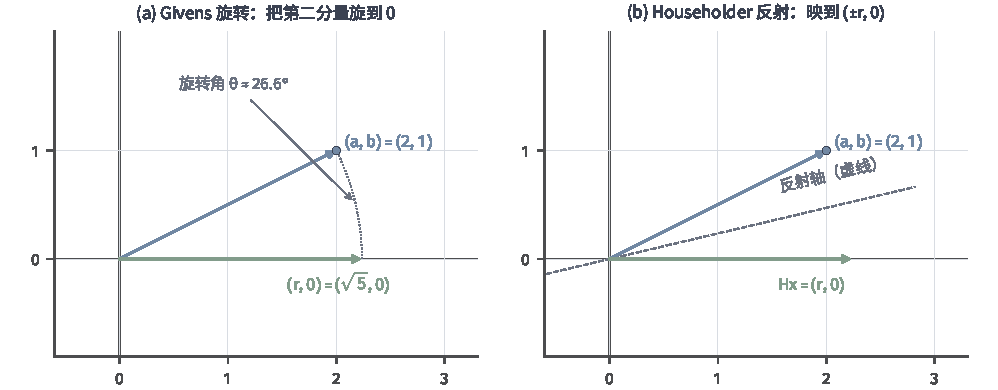
\includegraphics[width=168.998mm]{figures/01-mathematical-preliminaries-upper/02-linear-spaces/matplotlib/ls-givens-householder-elimination/ls-givens-householder-elimination.pdf}
  \caption{两种初等正交消元。左：Givens旋转把$(a,b)=(2,1)^\top$沿圆弧旋到
  $(r,0)^\top$，$r=\sqrt5$，旋转角$\theta=\arctan(1/2)$；右：Householder反射沿角平分线
  把同一向量映到$(r,0)^\top$。两者都是正交变换，保持长度，区别在旋转（行列式$+1$）与
  反射（对称正交）。解析式教学构造。}
  \label{fig:ls-givens-householder-elimination}
\end{figure*}

稠密$m\times d$矩阵的QR约需$2md^2-2d^3/3$次基本浮点运算，
正交列可由反射向量隐式保存，多个右端可以复用全部反射与$\bm R$，
新增一列只需对已有$\bm Q$追加一次投影与正交化，不必整体重做。
稀疏情形按非零结构只触碰局部元素，Givens适合这种逐元素增量更新。
秩亏时QR表示仍然成立，但回代与秩判断需要列置换（选最大模列提前作主元）等补充手段，
判定小$\lvert r_{j,j}\rvert$是数值精度问题而非精确代数结论，阈值与扰动由后续章节
说明。经济型QR只保留$r$列$\bm Q$，节省$m-r$列存储。

\subsubsection{最近点计算}

把候选点写成$\bm p=\bm B\bm c$。存在性一节的反向判据把
“最小距离”换成可直接检验的正交条件：最近点的残差$\bm r=\bm y-\bm B\bm c$必须与
每个基向量$\bm b_i$正交。这个条件不要求预先知道最小值，也不要求对$\bm c$逐点
比较距离，只要求列出$\dim U$个正交方程，把连续最小化变成线性系统求解；它是
可直接核验的一阶条件，满足时由勾股恒等式自动保证全局最小。几何上，残差垂直落
到$U$上，垂足即最近点。

\paragraph{正交残差条件与Gram系统}

标准内积下条件为$\bm B^\top(\bm y-\bm B\bm c)=\bm0$，即
\begin{equation}
 \bm G\bm c=\bm B^\top\bm y,\qquad
 g_{i,j}=\langle\bm b_i,\bm b_j\rangle.
 \label{eq:ls-gram-system}
\end{equation}
逐行写就是$\sum_j\langle\bm b_i,\bm b_j\rangle c_j=\langle\bm b_i,\bm y\rangle$，
即残差与每个基向量正交的$\dim U$个方程。加权内积下改为
$\bm B^\top\bm M(\bm y-\bm B\bm c)=\bm0$，Gram矩阵换成$\bm B^\top\bm M\bm B$。
\ref{sec:ls-orthogonality}已说明：基向量线性无关时，对任意非零$\bm c$有
$\bm c^\top\bm G\bm c=\lVert\bm B\bm c\rVert_2^2>0$，故$\bm G$正定、系统可逆。
边界：若基相关，$\bm G$奇异，方程仍相容但系数不唯一，最近点作为点仍唯一。

$\bm G$正定时方程~\eqref{eq:ls-gram-system}有唯一解$\bm c$，
对应唯一最近点$\bm p=\bm B\bm c$；权重$\bm M$正定时加权Gram矩阵
$\bm B^\top\bm M\bm B$同样正定（对非零$\bm c$有
$\bm c^\top\bm B^\top\bm M\bm B\bm c=\lVert\bm B\bm c\rVert_{\bm M}^2>0$），
同一结论保持。基相关时$\bm G$奇异、系数不唯一（同一$\bm p$
有多种组合），但最近点$\bm p$作为$U$中的点仍唯一，只需要再按准则选系数代表；
例如$\bm b_2=2\bm b_1$时，$\bm p=\bm b_1$可写成$\bm c=(1,0)$或$(0,1/2)$，
点相同而系数不同。

由$\bm B=\bm Q\bm R$，$\bm R$可逆时$\bm p=\bm Q\bm Q^\top\bm y$：
先算$\bm Q^\top\bm y$，再解三角系统$\bm R\bm c=\bm Q^\top\bm y$恢复系数，
最后$\bm p=\bm B\bm c$。由于$\bm Q^\top\bm Q=\bm I$，
$\bm Q^\top\bm y$的分量就是各正交方向上的坐标，无需先解Gram系统。
这条路线不显式形成Gram矩阵；形成正规乘积造成的尺度损失由后续章节用条件数解释。

核验分三步：$\bm p=\bm B\bm c\in U$；残差$\bm r=\bm y-\bm p$与$\bm B$各列正交；
报告最小距离$\lVert\bm r\rVert_2$。加权内积改变最近点，例~\ref{ex:linear-algebra-weighted-projection}
在同一直线上比较两种度量。
\begin{example}[同一子空间的两种最近点]
\label{ex:linear-algebra-weighted-projection}
在$\mathbb R^2$中取目标$\bm y=(2,1)^\top$、$U=\operatorname{span}\{(1,1)^\top\}$，
最近点写成$a(1,1)^\top$。欧氏投影最小化$(2-a)^2+(1-a)^2$，
导数给出$2a=3$，故$\bm p=(1.5,1.5)^\top$。
改用$\bm M=\operatorname{diag}(1,4)$，目标函数为$(2-a)^2+4(1-a)^2$，
导数给出$10a=12$，即$5a=6$，得到$\bm p_{\bm M}=(1.2,1.2)^\top$。
第二坐标误差代价更大，最近点便向$b_2=1$靠近；
残差$(0.8,-0.2)^\top$与$(1,1)^\top$的普通内积为$0.6\neq0$，
加权内积$0.8\cdot1+4(-0.2)\cdot1=0$，正交性必须用所选内积判断。
\end{example}
\begin{figure*}[htbp]
  \centering
  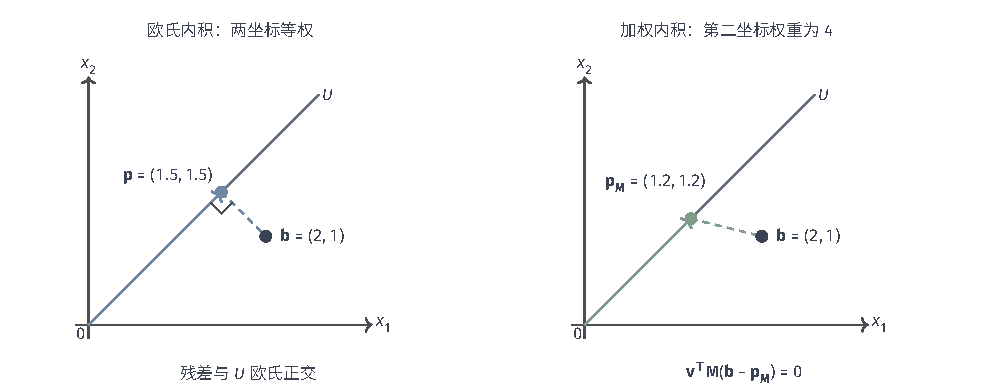
\includegraphics[width=168.998mm]{figures/01-mathematical-preliminaries-upper/02-linear-spaces/tikz/linear-algebra-weighted-projection/figure.pdf}
  \caption{同一目标在同一直线上的欧氏投影与加权投影。实箭头是投影向量，虚线是残差；
  右图画在普通坐标中，残差不必形成欧氏直角。正交性必须用所选内积判断。}
  \label{fig:linear-algebra-weighted-projection}
\end{figure*}

\subsection{投影的性质}

\paragraph{正交投影、斜投影与幂等}

标准内积下，以$\bm Q$为标准正交基的正交投影为
\begin{equation}
 \bm P_U=\bm Q\bm Q^\top,\qquad
 \bm P_U^\top=\bm P_U,\qquad \bm P_U^2=\bm P_U.
 \label{eq:linear-algebra-orthogonal-projector}
\end{equation}
它同时满足三条可逐条核验的性质：
\begin{enumerate}
 \item \term{幂等}（idempotent）：$\bm P_U^2=\bm Q\bm Q^\top\bm Q\bm Q^\top=\bm Q\bm Q^\top$，
 作用两次等于作用一次。
 \item 自伴（标准内积下$\bm P_U^\top=\bm P_U$）：保证残差与像正交，即欧氏最近点。
 \item 像为$U$：$\operatorname{range}\bm P_U=\operatorname{range}\bm Q=U$。
\end{enumerate}
但一般幂等映射只是沿某个方向把空间投到像上，
残差不必与像正交，也未必是最近点，这种映射称为\term{斜投影}（oblique projection）；
只有自伴的幂等映射才是正交投影。
例如$\bm P=\left[\begin{smallmatrix}1&-1\\0&0\end{smallmatrix}\right]$满足
$\bm P^2=\bm P$，把$(x,y)^\top$投到$x$轴上的$(x-y,0)^\top$，但
$\bm P^\top\neq\bm P$，残差$(y,y)^\top$不与$x$轴正交（普通内积$y\cdot0+y\cdot1=y\neq0$），
因而不是欧氏最近点。判别顺序：先验幂等（是否投影），再验对称（是否正交），
不能见幂等就当作最近点映射。

两个正交投影的复合一般不可交换：$\bm P_U\bm P_V\neq\bm P_V\bm P_U$，
乘积也未必仍是投影（两次投影的像一般既不是$U$也不是$V$）。两者可交换时，乘积
幂等且自伴，其像为$U\cap V$。反复投影怎样收敛到交空间属于序列极限问题，
留给后续收敛章节分析，这里不声称一次复合给出极限。

\section{线性方程：精确求解}
\label{sec:ls-exact-linear-equations}
\label{sec:linear-algebra-exact-systems}

\subsection{方程与条件}

给定$\bm A\in\mathbb R^{m\times d}$与目标$\bm b\in\mathbb R^m$，精确方程为
\begin{equation}
 \bm A\bm x=\bm b,\qquad \bm x\in\mathbb R^d.
 \label{eq:linear-algebra-linear-system}
\end{equation}
多个右端写成$\bm A\bm X=\bm B$，$\bm X\in\mathbb R^{d\times s}$、$\bm B\in\mathbb R^{m\times s}$；
它逐列等价于$s$个同系数矩阵的单右端方程$\bm A\bm x_j=\bm b_j$。
同一个$\bm A$的分解或迭代设置可按列复用，但每一列的相容性与残差要分别核验，
不能用一列的残差代替另一列。

按形状分：$m=d$为方阵，$m>d$为超定（方程多于未知量），$m<d$为欠定。
形状只限制秩的上限，不能单独判断有没有解：例如$\bm A=\left[\begin{smallmatrix}1\\1\end{smallmatrix}\right]$
是超定系统，但$\bm b=(1,1)^\top$在列空间内，因而相容且唯一；
而两行相同的方阵$\bm A=\left[\begin{smallmatrix}1&1\\1&1\end{smallmatrix}\right]$配
$\bm b=(1,2)^\top$就不相容。是否存在解由右端与值域的关系决定，
是否唯一由零空间决定，下面先判这两件事。

本节要求等式严格成立；浮点计算中“精确”表现为残差小到
给定容限，容限取值、舍入积累与条件数由后续章节处理。这里先在代数层面区分无解、
唯一解与多解，不能由某个算法算不出解就推断问题无解——算法失败可能只是数值或
实现问题，与代数相容性是两回事。

\subsection{存在性、唯一性与选解}

\subsubsection{相容性}
\label{sec:ls-compatibility}

$\bm A\bm x$是$\bm A$各列以$\bm x$为系数的线性组合，因此
$\bm A\bm x=\bm b$有解当且仅当$\bm b\in\operatorname{range}(\bm A)
=\operatorname{span}\{\bm a_1,\ldots,\bm a_d\}$。这一条件称为\term{相容}
（consistent）；不相容时任何输入都不能精确产生$\bm b$。判据直接来自列空间定义：
可达输出恰好是列的全部线性组合。例如$\bm A=\left[\begin{smallmatrix}1&1\\0&1\end{smallmatrix}\right]$，
两列$(1,0)^\top,(1,1)^\top$线性无关，列空间是全$\mathbb R^2$，任意右端都可达；
若把第二列换成$(1,1)^\top$使两列相同，列空间只是一条直线，垂直于它的右端就
不可达。形状（方程数多少）不决定可达性，列张成的空间才决定。

标准内积下有四个基本子空间：值域$\operatorname{range}(\bm A)$
与零空间$\operatorname{null}(\bm A)=\{\bm x:\bm A\bm x=\bm0\}$，
行空间$\operatorname{range}(\bm A^\top)$与左零空间
$\operatorname{null}(\bm A^\top)=\{\bm y:\bm A^\top\bm y=\bm0\}$。
由\ref{sec:ls-adjoints}建立的伴随恒等式
$\langle\bm y,\bm A\bm x\rangle=\langle\bm A^\top\bm y,\bm x\rangle$
是下面正交互补关系的依据：它把输出空间的配对转成输入空间的配对，使两个正交
关系不必另行假设。四个子空间分属输入、输出两个空间，不要混在同一侧。

若$\bm y\in\operatorname{null}(\bm A^\top)$，则对任意$\bm x$有
$\bm y^\top(\bm A\bm x)=(\bm A^\top\bm y)^\top\bm x=0$，故
$\operatorname{null}(\bm A^\top)\subseteq\operatorname{range}(\bm A)^\perp$；
维数互补给出反向包含，于是
\begin{equation}
 \operatorname{range}(\bm A)^\perp=\operatorname{null}(\bm A^\top).
 \label{eq:ls-range-leftnull-orthogonal}
\end{equation}

同理，$\operatorname{range}(\bm A^\top)^\perp
=\operatorname{null}(\bm A)$：若$\bm x\in\operatorname{null}(\bm A)$，则对任意
$\bm A^\top\bm y$有$(\bm A^\top\bm y)^\top\bm x=\bm y^\top\bm A\bm x=0$，
反向包含由维数互补得到。输入空间因此正交直和分解为
$\operatorname{null}(\bm A)\oplus\operatorname{range}(\bm A^\top)$，
输出空间分解为$\operatorname{range}(\bm A)\oplus\operatorname{null}(\bm A^\top)$。
前者记录被映射消去的输入方向，后者记录达不到的输出方向。

$\bm A\bm x=\bm b$相容的几何判据是$\bm b\in\operatorname{range}(\bm A)$，
即$\bm b$落在列空间内。等价地，由式~\eqref{eq:ls-range-leftnull-orthogonal}，
$\bm b$与左零空间正交：$\bm y^\top\bm b=0$对一切$\bm y\in\operatorname{null}(\bm A^\top)$
成立。前面的最近点结果将用于：不相容时求离$\bm b$最近的可达输出，
这是后续最小二乘任务的入口；本节只在相容前提下求精确解，不做残差最小化，
也不把“最近点”冒充为“解”。判据对任意形状的$\bm A$都适用，与$m,d$谁大无关。

\paragraph{增广矩阵的秩判据}

把$\bm b$并入系数矩阵得到增广矩阵$[\bm A\;\bm b]$。
$\bm b$是列的组合，当且仅当并入它不增加列空间维数，即
\begin{equation}
 \operatorname{rank}[\bm A\;\bm b]=\operatorname{rank}(\bm A).
 \label{eq:ls-augmented-rank}
\end{equation}
这是消元可直接检验的代数判据；不等号出现即无解。理由：若$\bm b$已在列空间内，
并入不扩大张成空间，秩不变；否则秩增加一。例如
$\bm A=\left[\begin{smallmatrix}1&1\\1&1\end{smallmatrix}\right]$的秩为$1$，
$\bm b=(1,2)^\top$使$[\bm A\;\bm b]$秩为$2$，判据直接给出无解；
而$\bm b=(1,1)^\top$并入后秩仍为$1$，相容。

不相容可由左零空间直接证明：若存在
$\bm y\in\operatorname{null}(\bm A^\top)$使$\bm y^\top\bm b\neq0$，
则所有可达输出$\bm A\bm x$在$\bm y$方向读数为
$\bm y^\top\bm A\bm x=(\bm A^\top\bm y)^\top\bm x=0$，而$\bm b$非零，
故$\bm b$不可达。上例中$\bm y=(1,-1)^\top$满足
$\bm A^\top\bm y=0$，而$\bm y^\top\bm b=1-2=-1\neq0$，这就是不可达证书。
反之，$\bm y^\top\bm b=0$对全部$\bm y\in\operatorname{null}(\bm A^\top)$
成立时，由式~\eqref{eq:ls-range-leftnull-orthogonal}知$\bm b$与左零空间正交，
即$\bm b\in\operatorname{range}(\bm A)$。证书法与秩判据等价，但给出一个可
直接核验的向量。

$\bm A\bm X=\bm B$相容当且仅当每一列
$\bm b_j\in\operatorname{range}(\bm A)$，等价于
$\operatorname{rank}[\bm A\;\bm B]=\operatorname{rank}(\bm A)$，
也等价于所有$\bm y\in\operatorname{null}(\bm A^\top)$满足$\bm y^\top\bm B=\bm0$。
各列独立判断，不能用一列相容代替另一列；逐列残差分别核验。

\subsubsection{唯一性与自由度}
\label{sec:ls-uniqueness-freedom}

设$\bm x_1,\bm x_2$都是解，则
$\bm A(\bm x_1-\bm x_2)=\bm b-\bm b=\bm0$，两解之差属于零空间
$\operatorname{null}(\bm A)$；反之，若$\bm x_0$是解且
$\bm n\in\operatorname{null}(\bm A)$，则$\bm A(\bm x_0+\bm n)=\bm b+\bm0=\bm b$，
故$\bm x_0+\bm n$也是解。这一双向关系说明：解集合恰好是“一个特解平移零空间”，
没有其他点混入。

\paragraph{特解加零空间的全部解}

相容时任取一个特解$\bm x_0$，全部解恰为
\begin{equation}
 \bm x=\bm x_0+\operatorname{null}(\bm A).
 \label{eq:ls-affine-solution-set}
\end{equation}
这是一个平移后的线性子空间，即\term{仿射空间}（affine space）：基点$\bm x_0$
不唯一，更换基点只平移集合，方向空间$\operatorname{null}(\bm A)$由全部点差唯一确定。
商空间把这种不可区分性表达为精确对应：
$\mathbb R^d/\operatorname{null}(\bm A)\to\operatorname{range}(\bm A)$，
$\bm x+\operatorname{null}(\bm A)\mapsto\bm A\bm x$良定义、线性、单射且满射，
却尚未在每个类中选代表。例如$x_1+x_2=2$有特解$(1,1)^\top$，零空间由
$(1,-1)^\top$张成，全部解为$(1,1)^\top+t(1,-1)^\top$，$t$任意；
$(1,0)^\top$与$(0,1)^\top$在$\bm A=(1,1)$下同属一类、只记录系数和。
\label{sec:linear-algebra-affine-relations}
图~\ref{fig:vol1-add-linear-nullspace-fibers}以$\bm A=(1,1)$展示：每条平行线
$x_1+x_2=c$对应同一个输出数，整条线归为一个原像类。
\begin{figure}[!htb]
  \centering
  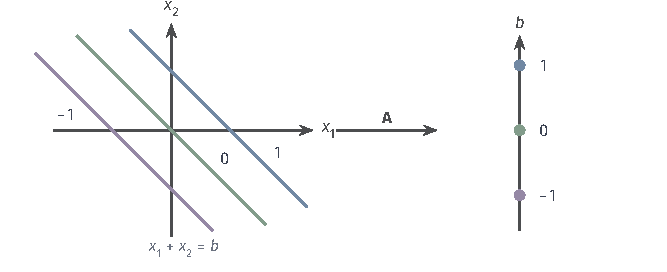
\includegraphics[width=112mm]{figures/01-mathematical-preliminaries-upper/02-linear-spaces/tikz/comprehension-additions/linear-nullspace-fibers.pdf}
  \caption{同一输出对应的整组输入。对$\bm A=(1,1)$，蓝、绿、紫直线分别满足
  $x_1+x_2=1,0,-1$；右侧同色点是各直线的输出。绿色直线是$\ker\bm A$，
  其余直线是它的平移。把一整条直线归为一类后，才得到与可达输出的一一对应。}
  \label{fig:vol1-add-linear-nullspace-fibers}
\end{figure}

由秩零度定理~\ref{thm:ls-rank-nullity}，
$\dim\operatorname{null}(\bm A)=d-\operatorname{rank}(\bm A)$，
这就是自由参数的个数。相容时任一特解$\bm x_0$加上零空间的全部点构成解集，
解集是$d-r$维仿射空间，$r=\operatorname{rank}(\bm A)$；
每增加一个自由参数，就多一个沿零空间移动而不改变输出的方向，自由参数个数
与列数减秩一致。例如$\bm A=[1\ 1]$，$d=2,r=1$，自由参数$1$个，
解$\bm x=(1,1)^\top+t(1,-1)^\top$中$t$即自由参数；$d-r=0$时零空间只含零向量，
自由参数为零，解唯一。

\paragraph{满列秩、满行秩与唯一性}

解唯一当且仅当$\operatorname{null}(\bm A)=\{\bm0\}$，
即满列秩$r=d$（$d$个列向量线性无关）：两解之差落在零空间，零空间为零向量迫使
两解相同。满行秩$r=m$只保证每个右端都可达（相容），
不保证唯一；满列秩保证唯一但不保证任意右端可达。两种满秩对应不同保证，
不能互换：满行秩可能欠定多解，满列秩可能超定不相容。例如$\bm A=(1,1)$满行秩
（$m=1$）但欠定，任意$\bm b$相容而解不唯一；$\bm A=(1,1)^\top$满列秩（$d=1$），
解唯一却只对$\bm b\in\operatorname{span}\{(1,1)^\top\}$相容。

超定$m>d$且满列秩时，相容则唯一解，不相容则无精确解（此时进入残差最小化任务）；
欠定$m<d$且满行秩时任意右端都相容，但至少有$d-m$个自由参数，解不唯一。
仅凭方程数与未知数个数不能下结论，必须回到实际秩与右端位置：超定也可能相容唯一，
方阵也可能无解。例如方阵$\bm A=\left[\begin{smallmatrix}1&1\\1&1\end{smallmatrix}\right]$
秩$1<d=2$，既多解又对$\bm b\notin\operatorname{span}\{(1,1)^\top\}$无解，
形状为方阵却不具备可逆性。

$\bm A=\bm0$时：$\bm b=\bm0$则任意$\bm x$都是解
（零空间为全空间$\mathbb R^d$，列空间为$\{0\}$），$\bm b\neq\bm0$则无解
（零右端落在列空间$\{0\}$内，非零右端不在）。反过来$\bm b=\bm0$而$\bm A\neq0$
时齐次方程$\bm A\bm x=\bm0$恒相容，至少有零解，秩亏时另有非零解。
这种边界不能套用含零分母的求逆公式（$\bm A^{-1}$不存在），直接按上述秩与值域
判据判断，避免对零矩阵作除法。

\subsubsection{多解中的选择}
\label{sec:ls-select-among-solutions}

相容而秩亏时，全部解是$\bm x_0+\operatorname{null}(\bm A)$，
等式本身不再挑选代表，需要额外准则。常用的是在解集中取欧氏范数最小者；
更换输入内积，代表点一般随之改变，准则必须先声明，不能默认“解”唯一。
这一准则与6.1的最近点几何一致：在平移仿射集合上找离原点最近的点，
垂足落在零空间的正交补上。

把任意解按输入空间的正交直和分解为
$\bm x=\bm x_\perp+\bm x_N$，其中$\bm x_N\in\operatorname{null}(\bm A)$，
$\bm x_\perp\in\operatorname{null}(\bm A)^\perp=\operatorname{range}(\bm A^\top)$。
$\bm A\bm x_N=\bm0$，输出只由$\bm x_\perp$决定，核分量对输出毫无贡献；
两个分量正交，故可分开处理。

\paragraph{最小范数精确解的唯一性}

两项正交，故
$\lVert\bm x\rVert_2^2=\lVert\bm x_\perp\rVert_2^2+\lVert\bm x_N\rVert_2^2$。
保持$\bm x_\perp$不变而去掉$\bm x_N$，输出不变（$\bm A\bm x_N=0$）且范数
严格减小；唯一最小范数代表就是$\bm x_N=0$的那个解，它落在
$\operatorname{null}(\bm A)^\perp$中。上例$x_1+x_2=2$的解
$(1+t,1-t)^\top$中，范数平方为$(1+t)^2+(1-t)^2=2+2t^2$，令核分量$t=0$
得$(1,1)^\top$，其范数$\sqrt2$小于$t\neq0$时的$\sqrt{2+2t^2}$。
映射$\bm A|_{\operatorname{null}(\bm A)^\perp}:
\operatorname{null}(\bm A)^\perp\to\operatorname{range}(\bm A)$是双射：
单射来自交为零，满射来自上述分解，故最小范数代表存在且唯一。

满列秩时$\bm A^\top\bm A$正定，存在左逆
$\bm L=(\bm A^\top\bm A)^{-1}\bm A^\top$使$\bm L\bm A=\bm I$，
它能恢复全部输入，但只对值域中的输出反演；满行秩时存在右逆
$\bm R=\bm A^\top(\bm A\bm A^\top)^{-1}$使$\bm A\bm R=\bm I$，
它为每个输出挑一个输入，却不能恢复被零空间消去的信息。单侧逆一般不唯一：
例如$\bm A=(1,0)^\top$，任意$\bm L=(1,t)$都满足$\bm L\bm A=1$，
$t$任意而不破坏左逆。它们是代数公式，实际通过三角求解应用，不显式形成逆矩阵；
左逆对应唯一解（满列秩），右逆对应一种选解（满行秩）。

最小范数代表依赖指定的输入内积；一般权重或正则化会同时改变目标与代表，
完整的伪逆构造、任意秩处理与加权选解放在后续残差最小一节。本节只确认：多解时等式不唯一，
必须先声明准则再谈“解”；在未声明准则前，报告“一个解”而非“那个解”。
满行秩右逆给出的代表只是众多选解之一，未必是最小范数代表，二者不可混称。

\subsection{直接法}
\label{sec:ls-direct-methods}
\label{sec:linear-algebra-direct-exact}
\label{sec:matrix-analysis-stable-solvers}

直接法在有限步内把方程化为可逐个求解的三角或块系统。它需要显式读取并存储因子，
适用于矩阵可整体获得、规模可控或多右端复用同一因子的情形。

\subsubsection{消元与LU分解}

高斯消元用一行的倍数消去另一行的某个系数，
行变换（把某行加到另一行、交换两行、某行乘非零常数）不改变解集。例如
$\left[\begin{smallmatrix}2&1\\4&3\end{smallmatrix}\right]\bm x=(1,3)^\top$，
第二行减去第一行的两倍得$(0,1)$对应$x_2=1$，再代回$2x_1+1=1$得$x_1=0$。
多步消元记录下来就是三角因子，不必每次从头回代。

第$k$步在尚未处理的第$k$列中选择绝对值最大的可用元素移到主元位置，
再消去它下方的元素；记录的行交换累计为置换矩阵$\bm P$。例如主元位置为零而其下方
同列有非零元时，交换两行即可继续；部分主元避免把本可交换避开的零元素拿来作除数，
也抑制乘子$l_{i,k}=a_{i,k}/a_{k,k}$过大带来的放大。但交换不会把奇异矩阵变成
可逆矩阵：秩由列张成决定，行置换只重排方程，不改变秩与相容性。

\paragraph{消元乘子与LU因子}

消去乘子$l_{i,k}=a^{(k)}_{i,k}/a^{(k)}_{k,k}$进入单位下三角
因子$\bm L$，剩余系数构成上三角因子$\bm U$，得到带部分主元的分解
\begin{equation}
 \bm P\bm A=\bm L\bm U,
 \label{eq:matrix-analysis-palu}
\end{equation}
其中$\bm L$单位下三角（对角为1）、$\bm U$上三角。乘子就是第$k$步消去第$i$行
第$k$列所用的倍数，被原样留在$\bm L$中，使$\bm L\bm U$乘回可复原置换后的
系数矩阵；前面列的乘子随行交换同步更新。验证方式：把$\bm L\bm U$逐项乘回，
与$\bm P\bm A$比较，不必另行求解。

消元得到的阶梯形直接显示秩：每选到一个非零主元秩加一；精确算术中某列无可用主元，
说明矩阵秩亏，此时应转入秩判断并按6.2.1相容性判据核验增广矩阵秩，而不是继续
除以零。对相容的秩亏系统，自由变量取零即得一个特解，其余解沿零空间展开；
对不相容系统，阶梯形会出现$0=\text{非零}$的矛盾行，直接判定无解。
某个小主元不能独自证明精确奇异，浮点阈值决定的数值秩留待后续章节说明；
代数上的奇异（主元恰为零）与数值上的接近奇异（主元很小但非零）是两件事。

分解后依次解$\bm L\bm z=\bm P\bm b$（前代，从前向后）与
$\bm U\bm x=\bm z$（回代，从后向前）：
\begin{equation}
 z_i=(\bm P\bm b)_i-\sum_{j<i}l_{i,j}z_j,\qquad
 x_i=\frac{z_i-\sum_{j>i}u_{i,j}x_j}{u_{i,i}}.
\end{equation}
回到开头的例子，消元后$\bm U=\left[\begin{smallmatrix}2&1\\0&1\end{smallmatrix}\right]$、
$\bm L=\left[\begin{smallmatrix}1&0\\2&1\end{smallmatrix}\right]$，
先由$\bm L\bm z=(1,3)^\top$得$z_1=1$、$z_2=1$，再回代$x_2=1$、
$2x_1+1=1$得$x_1=0$。解出后代回原方程核验$\bm A\bm x=\bm b$。

因子$\bm L,\bm U$（或置换$\bm P$）只建立一次，每个新右端$\bm b_j$各自完成两次
三角求解$\bm L\bm z_j=\bm P\bm b_j$、$\bm U\bm x_j=\bm z_j$，不必为每列重做
$O(d^3)$分解；当同一$\bm A$搭配多列$\bm B$时，分摊成本主要落在$O(d^2)$的逐列
三角求解上。矩阵改变后不能无条件复用旧因子：结构或元素变化使$\bm L\bm U$不再等于
新的$\bm P\bm A$，须重新分解；仅有右端变化才允许复用。

稠密$d\times d$矩阵的LU分解约需$2d^3/3$次基本浮点运算，
每个新右端的两次三角求解为$O(d^2)$，存储$O(d^2)$。稀疏矩阵消元可能产生原来
没有的非零元，称为\term{填充}（fill-in），使原本稀疏的因子退化为准稠密；
存储收益还取决于行列排序与结构，而不只看原始非零元数。因此稀疏直接法的成本
不能只用原始非零元数估计。

\subsubsection{Cholesky分解}

当$\bm A=\bm A^\top\succ0$（对称正定）时，
定理~\ref{thm:ls-gram-factor}的配方原理已说明正定矩阵可归纳写成$\bm L\bm L^\top$
形式；本节把它落实为可逐列执行的三角求解算法。Cholesky 能省去 LU 的选主元，前提可拆成
三条同时成立：
\begin{enumerate}
 \item 对称性$\bm A=\bm A^\top$：只需存储一个三角因子，配方只作用于上半。
 \item 正定性$\bm x^\top\bm A\bm x>0$（$\bm x\neq\bm0$）：等价于各阶顺序主子式为正，
 配方剩余$a_{j,j}-\sum_{k<j}l_{j,k}^2>0$恒成立。
 \item 由此每步主元严格为正：无需行交换，不会出现零主元或负数开方。
\end{enumerate}
这是它相对LU的简化前提。

把第一个坐标与其余坐标分块配方，消去首变量后剩余的系数矩阵
仍正定，因而每一步的主元严格为正；按维数归纳即可逐列构造因子。具体地，正定二次型
对首变量配成完全平方，平方项系数为正，余下不含首变量的二次型由正定性仍正定，
这也解释了Cholesky每步剩余矩阵为何保持正定结构、根号内为何严格为正。这一归纳
正是定理~\ref{thm:ls-gram-factor}配方原理的逐步执行，不是另立假设。

\paragraph{Cholesky因子的逐列构造}

存在唯一对角元为正的下三角矩阵$\bm L$使
\begin{equation}
 \bm A=\bm L\bm L^\top,
 \label{eq:matrix-analysis-cholesky}
\end{equation}
称为\term{Cholesky分解}（Cholesky decomposition）。逐列计算
\begin{equation}
 l_{j,j}=\sqrt{a_{j,j}-\sum_{k<j}l_{j,k}^2},\qquad
 l_{i,j}=\frac{a_{i,j}-\sum_{k<j}l_{i,k}l_{j,k}}{l_{j,j}}\quad(i>j).
\end{equation}
第一式是第$j$个对角平方（配方剩余），第二式由$\bm L\bm L^\top$的$(i,j)$元
$a_{i,j}=\sum_{k\leq j}l_{i,k}l_{j,k}$反解得到。正定性保证根号内严格为正，
除法合法。例如$\bm A=\left[\begin{smallmatrix}4&2\\2&5\end{smallmatrix}\right]$，
先得$l_{11}=\sqrt4=2$，再$l_{21}=a_{21}/l_{11}=2/2=1$，最后
$l_{22}=\sqrt{5-l_{21}^2}=\sqrt{5-1}=2$，故
$\bm L=\left[\begin{smallmatrix}2&0\\1&2\end{smallmatrix}\right]$，
乘回$\bm L\bm L^\top=\left[\begin{smallmatrix}4&2\\2&5\end{smallmatrix}\right]$
逐项等于原矩阵。

每列由先前列唯一确定：式~\eqref{eq:matrix-analysis-cholesky}的$(i,j)$元给出
$a_{i,j}=\sum_{k\leq j}l_{i,k}l_{j,k}$，右侧$k<j$项已由先前因子确定，故$l_{i,j}$
被唯一反解；对角$l_{j,j}$由配方剩余开方，正对角约定又固定了开方符号（取$+$而非$-$），
因此带正对角的Cholesky分解唯一。若允许对角取负号，$\pm l_{j,j}$都满足乘积，符号未定，
正对角约定排除了这一任意性。对照LU：一般矩阵的LU在主元非零时也唯一，
而Cholesky额外靠正定性保证根号内为正、无需选主元。

求解依次用$\bm L\bm z=\bm b$（前代，$z_i=(b_i-\sum_{j<i}l_{i,j}z_j)/l_{i,i}$）与
$\bm L^\top\bm x=\bm z$（回代，$x_i=(z_i-\sum_{j>i}l_{j,i}x_j)/l_{i,i}$）。
稠密成本约$d^3/3$，只存一个三角因子（利用对称不复存上半），
约为LU的一半；多个右端复用同一因子，每个右端仍需两次三角求解$O(d^2)$。
复用前提仍是$\bm A$不变。

半正定时可能出现零主元（配方剩余为零），不能照搬上述除以$l_{j,j}$与开正根号的
步骤，否则$0/0$或负数开方。盲目加一个“小常数”会改变原方程、把退化系统改成另一
问题；应先区分真实退化（$\bm A$本有零空间、相容前提下进入选解）、约束造成的零空间
与数值误差（接近奇异而非精确奇异，阈值问题留后续章节）。只有任务本身明确引入阻尼
或惩罚时，才改用相应的正则化系统，不能为让算法通过而临时改动系数。

\subsubsection{LDL$^{\top}$分解}
\label{sec:ls-ldlt}

对称但不定（有正也有负方向）的矩阵不能逐项开正平方根：它既没有Cholesky所需的
正主元可开正根号，也没有CG所需的正分母，二者都不能沿用；例如$\operatorname{diag}(1,-1)$可逆却出现负主元，
$\sqrt{-1}$无实意义。对称结构仍然保留，可把符号和耦合
留在对角块中，这正是LDL$^{\top}$分解的用途：不开方、由$\bm D$的负块承接符号。

引入带对称置换的分解$\bm P\bm A\bm P^\top=\bm L\bm D\bm L^\top$，
其中$\bm L$单位下三角，$\bm D$由一阶与二阶对角块组成。
例如$\left[\begin{smallmatrix}0&1\\1&0\end{smallmatrix}\right]$可逆却没有可用的一阶对角主元；
同时交换行列以保留对称性，选择可逆的一阶或二阶块作主元，再消去与剩余变量的耦合。

\paragraph{LDL$^{\top}$因子的形成}

按块递归消去耦合。把当前待消矩阵分块为
$\begin{bmatrix}\bm A_{11}&\bm A_{12}\\\bm A_{21}&\bm A_{22}\end{bmatrix}$，
其中$\bm A_{11}$是选定的可逆一阶或二阶块；单位下三角乘子块取
$\bm L_{21}=\bm A_{21}\bm A_{11}^{-1}$，消去后剩余块为Schur补
$\bm A_{22}-\bm A_{21}\bm A_{11}^{-1}\bm A_{12}$，再对剩余块重复同一过程。
$\bm L$记录这些乘子（单位对角），$\bm D$保留各步选定的对角块（一阶标量或二阶
对称块）。不定矩阵的负主元不是算法失败，只是不能开平方；$\bm D$的负块直接
保留符号。每步乘回$\bm L\bm D\bm L^\top$逐项核对，确认乘积等于置换后的系数矩阵。
与Cholesky相比，LDL$^{\top}$不开根号、把符号集中在$\bm D$，因此可覆盖对称不定
与条件良好的半定情形；$\bm D$为一阶、二阶块正是为了在无正主元时仍取得可逆块。

一阶块$d$直接除以标量$d$：$y=z/d$。二阶块
$\begin{smallmatrix}d_{11}&d_{12}\\d_{12}&d_{22}\end{smallmatrix}$
解$\bm D\bm y=\bm z$，令$\Delta=d_{11}d_{22}-d_{12}^2$（非零由块主元可逆保证），
则
\begin{equation}
 y_1=\frac{d_{22}z_1-d_{12}z_2}{\Delta},\qquad
 y_2=\frac{d_{11}z_2-d_{12}z_1}{\Delta}.
\end{equation}
负对角元照常保留，不要求开平方；二阶块一次解完即可，不必再细分。例如二阶块
$\begin{smallmatrix}0&1\\1&0\end{smallmatrix}$（$d_{11}=0,d_{12}=1,d_{22}=0$）
行列式$\Delta=-1\neq0$，代入得$y_1=z_2$、$y_2=z_1$，直接解出两个未知量，
避免了寻找不存在的一阶零对角主元。

求解依次经过置换（把右端按$\bm P$重排）、下三角系统$\bm L\bm z=\bm P\bm b$
（前代）、小对角块系统$\bm D\bm y=\bm z$（逐块解一阶/二阶）和上三角系统
$\bm L^\top\bm x=\bm y$（回代），最后按置换$\bm P^\top$恢复原坐标；
每一步都是易解的三角或小块系统，回代次序与消元相反，置换把被交换的列/行位置
还原。这一链条与Cholesky两次三角求解平行，只是中间插入块对角求解与逆置换。

区分“具有负方向”（不定、$\bm D$出现负块）和“具有零空间”（奇异、$\bm D$出现
零块）：前者仍可唯一求解，负块只是符号；后者需重新判断相容性与选解，不能把零块
当可逆块作除法。这里只说明结构与求解路径，求解驻点方程不等于最小化对应的二次目标
（不定二次型无下界，驻点不是极小点）。

\subsubsection{QR分解}

前面建立的QR用正交变换把$\bm A$化为上三角。正交变换
保持欧氏长度，对相容方程$\bm A\bm x=\bm b$左乘$\bm Q^\top$后，方程拆成
可解的三角约束（前$d$行$\bm R\bm x=\bm Q^\top\bm b$）与自动满足的零残差行
（下方$\bm Q^\top\bm b$分量为零，这是相容条件$\bm b\in\operatorname{range}(\bm A)$
的投影表达），不需要额外极小化。不相容时下方残差非零，进入最小二乘任务而非本节。

$m\geq d$且满列秩时，经济型$\bm A=\bm Q\bm R$给出
$\bm R$可逆上三角；相容时解$\bm R\bm x=\bm Q^\top\bm b$，下方行的残差自动为零。
例如$\bm A=\left[\begin{smallmatrix}1&1\\1&0\\0&1\end{smallmatrix}\right]$，
两列线性无关；取相容右端$\bm b=(2,1,1)^\top=\bm A(1,1)^\top$。QR把$\bm A$
化为上三角，前两行$\bm R$可逆、第三行为零；左乘$\bm Q^\top$后第三行给出相容性核验
（此处$\bm Q^\top\bm b$第三分量为零），前两行的上三角系统回代得
$\bm x=(1,1)^\top$，代回$\bm A\bm x$得$(2,1,1)^\top=\bm b$。
若右端使第三分量非零，则方程不相容，转入后文最小二乘而非此处三角求解。

$m\leq d$且满行秩时对$\bm A^\top$作QR（即LQ分解，$\bm A=\bm L\bm Q^\top$），
在$\operatorname{range}(\bm A^\top)$内求解，使解落在零空间的正交补中，
自然得到最小范数方向上的代表。这与6.2.1“最小范数代表取在$\operatorname{null}(\bm A)^\perp$”
一致；转置QR只给满行秩情形一个选解路径，任意秩仍归SVD。

秩亏而相容时存在自由方向，解集为特解平移零空间；QR本身只给出一个满足方程的解，
不挑选最小范数代表。完整的任意秩选解工具（SVD，把解取在零空间正交补上）留待
后续残差最小章节，本节不声称普通QR已给出最小范数解。

列主元QR（QRCP）每步选模最大的未处理列提前作主元，重新安排列以辅助判断秩；
普通无主元QR的某个小对角元本身不是全部数值秩信息，可靠阈值还需要误差尺度
（条件数与扰动由后续章节给出）。无论用哪种QR，解出后仍须核验原方程残差
$\bm b-\bm A\bm x$，三角系统满足不等于原系统满足。

\subsubsection{分块消元与低秩更新}
\label{sec:matrix-analysis-blocks-updates}

先从最小的二元例子看消元在做什么。解
$\left[\begin{smallmatrix}2&1\\1&2\end{smallmatrix}\right](x_1,x_2)^\top=(1,3)^\top$：
第一式$2x_1+x_2=1$把$x_1=(1-x_2)/2$表示出来，代入第二式得
$(1-x_2)/2+2x_2=3$，乘$2$后$1+3x_2=6$，即$x_2=5/3$，回代$x_1=(1-5/3)/2=-1/3$。
核验：$2(-1/3)+5/3=1$、$(-1/3)+2(5/3)=3$。这里“用第一块消去第二块里的$x_1$”，
第二块剩下的系数$2-1\cdot(1/2)=3/2$，正是把$2\times2$矩阵左上元$2$作除后右下角的残留。
图~\ref{fig:ls-schur-block-elimination}把这一分块消元两步并置。

\begin{figure*}[htbp]
  \centering
  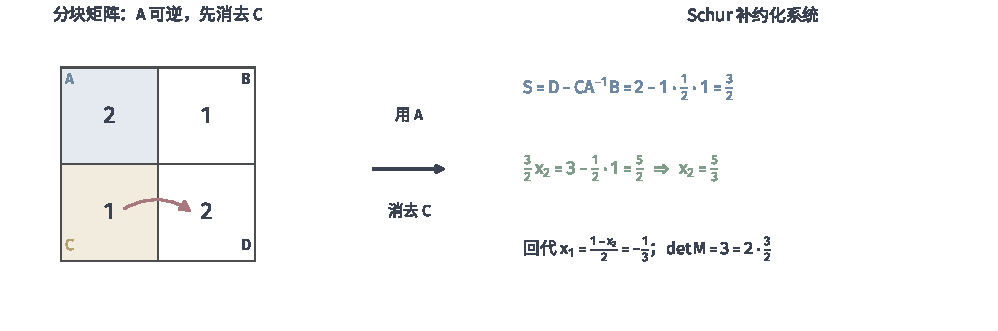
\includegraphics[width=168.998mm]{figures/01-mathematical-preliminaries-upper/02-linear-spaces/matplotlib/ls-schur-block-elimination/ls-schur-block-elimination.pdf}
  \caption{Schur 补的 2×2 分块消元。左：$\bm M=\left[\begin{smallmatrix}2&1\\1&2\end{smallmatrix}\right]$
  按左上块$\bm A=2$分块，先由第一行表出$x_1=(1-x_2)/2$；右：代入第二行后右下角残留
  Schur补$\bm S=3/2$，约化得$x_2=5/3$、回代$x_1=-1/3$，且$\det\bm M=2\cdot3/2=3$。
  解析式教学构造。}
  \label{fig:ls-schur-block-elimination}
\end{figure*}

下面把这一操作写成块记号。

把未知量分成两块，设
$\bm M=\left[\begin{smallmatrix}\bm A&\bm B\\\bm C&\bm D\end{smallmatrix}\right]$，
$\bm A\in\mathbb R^{p\times p}$可逆，右端$(\bm f^\top,\bm g^\top)^\top$。
第一组方程$\bm A\bm x+\bm B\bm y=\bm f$先把$\bm x=\bm A^{-1}(\bm f-\bm B\bm y)$
用$\bm y$表示，再代入第二组消去$\bm x$。典型来源是二部结构：全局参数块与各局部
块相连、局部块之间不直接相连，先分别消去各局部块，只剩全局块的小系统。

\paragraph{Schur补与约化系统}

\term{Schur补}（Schur complement）定义为
$\bm S=\bm D-\bm C\bm A^{-1}\bm B$。
\label{def:matrix-analysis-schur-complement}
代入第二组得到约化系统
\begin{equation}
 \bm S\bm y=\bm g-\bm C\bm A^{-1}\bm f,
 \label{eq:matrix-analysis-schur-complement}
\end{equation}
矩阵形式为
$\left[\begin{smallmatrix}\bm I&\bm0\\-\bm C\bm A^{-1}&\bm I\end{smallmatrix}\right]
\bm M=\left[\begin{smallmatrix}\bm A&\bm B\\\bm0&\bm S\end{smallmatrix}\right]$，
即左边乘一个单位下三角消去块左下角，把$\bm M$化成块上三角。在$\bm A$可逆
前提下，$\bm M$可逆当且仅当$\bm S$可逆，且$\det\bm M=\det\bm A\det\bm S$。
例如$\bm M=\left[\begin{smallmatrix}2&1\\1&2\end{smallmatrix}\right]$，
取$\bm A=2$、$\bm B=\bm C=1$、$\bm D=2$，则$\bm S=2-1/2=3/2$，
$\det\bm M=3=2\cdot3/2$，约化$3y/2=g-f/2$解出$y$后回代$x=(f-y)/2$。

解出$\bm y$后回代$\bm x=\bm A^{-1}(\bm f-\bm B\bm y)$。
逆通过求解$\bm A\bm Z=\bm B$、$\bm A\bm x=\bm f$来应用，不为套公式先形成整个
逆矩阵。需要时块逆为
\begin{equation}
 \bm M^{-1}=
 \begin{bmatrix}
  \bm A^{-1}+\bm A^{-1}\bm B\bm S^{-1}\bm C\bm A^{-1}
  &-\bm A^{-1}\bm B\bm S^{-1}\\
  -\bm S^{-1}\bm C\bm A^{-1}&\bm S^{-1}
 \end{bmatrix}.
 \label{eq:matrix-analysis-block-inverse}
\end{equation}
回代后必须代回原两块方程核验，约化系统相容不自动保证原方程每块满足。

$\bm M$对称时$\bm C=\bm B^\top$。配方给出
\begin{equation}
 \begin{bmatrix}\bm x\\\bm y\end{bmatrix}^{\top}
 \bm M\begin{bmatrix}\bm x\\\bm y\end{bmatrix}
 =(\bm x+\bm A^{-1}\bm B\bm y)^\top
 \bm A(\bm x+\bm A^{-1}\bm B\bm y)+\bm y^\top\bm S\bm y.
\end{equation}
右边两项分别为$\bm A$、$\bm S$的二次型。因此$\bm A\succ0$时
\begin{equation}
 \bm M\succ0\quad\Longleftrightarrow\quad
 \bm D-\bm B^\top\bm A^{-1}\bm B\succ0.
 \label{eq:matrix-analysis-schur-positive-definite}
\end{equation}
必要性可取$\bm x=-\bm A^{-1}\bm B\bm y$使第一项归零，只剩$\bm y^\top\bm S\bm y$
须对所有$\bm y$为正；充分性来自两项非负且不能同时为零（$\bm A$正定）。

对称正定等价于各阶顺序主子式为正，这正是逐块配方的主元；配方每步剩余矩阵正定，
故主元严格为正。半正定不能机械把严格不等号改为非严格，零主元对应真实退化，
主子式判据需另行处理零空间，不能套用正定除法；负主元（不定）则由LDL$^{\top}$
的块对角承接，不属Cholesky范围。

$\bm A$本身可能奇异，不能直接把$\bm A^{-1}$换成伪逆而不加条件；
需要$\operatorname{range}(\bm B)\subseteq\operatorname{range}(\bm A)$等值域条件
保证消去可行，以及伪逆版本的Schur补，再核验零空间是否留下自由参数。
不满足值域条件时，第一组方程$\bm A\bm x=\bm f-\bm B\bm y$对某些$\bm y$无解，
分块消元不能进行。

矩阵由$\bm A$变为$\bm A+\bm U\bm C\bm V^\top$，新增耦合只经过$k$个中间坐标
（$k$通常远小于$d$）。引入辅助未知量$\bm z=\bm V^\top\bm x$，把大系统换成$k$阶
小系统加已有$\bm A$的求解器，避免对$d$阶新矩阵重新分解；这是精确改变矩阵，不是
近似压缩，新矩阵与旧矩阵逐项不同。适用前提是旧求解器仍可用（$\bm A$可逆或已存
因子），$k$很小使小系统值得单独求解。

\paragraph{Woodbury恒等式与小系统}

设$\bm A$、$\bm C$与
$\bm S=\bm C^{-1}+\bm V^\top\bm A^{-1}\bm U$均可逆，按两种顺序消元同一块矩阵，
比较左上块得\term{Woodbury恒等式}
\begin{equation}
 (\bm A+\bm U\bm C\bm V^\top)^{-1}
 =\bm A^{-1}-\bm A^{-1}\bm U
 (\bm C^{-1}+\bm V^\top\bm A^{-1}\bm U)^{-1}
 \bm V^\top\bm A^{-1}.
 \label{eq:matrix-analysis-woodbury}
\end{equation}
取$\bm C=\bm I$时只需$\bm A$与$\bm I+\bm V^\top\bm A^{-1}\bm U$可逆，
无须对矩形$\bm U,\bm V$假定逆；实现为
$(\bm I+\bm V^\top\bm A^{-1}\bm U)\bm z=\bm V^\top\bm A^{-1}\bm b$，
再$\bm x=\bm A^{-1}(\bm b-\bm U\bm z)$。先消$\bm A$得小系统$\bm S$，
先消$\bm C^{-1}$得更新矩阵，两种消元左上块比较即得恒等式。

$k=1$时得Sherman--Morrison公式
$(\bm A+\bm u\bm v^\top)^{-1}
=\bm A^{-1}-\dfrac{\bm A^{-1}\bm u\bm v^\top\bm A^{-1}}
{1+\bm v^\top\bm A^{-1}\bm u}$，要求$1+\bm v^\top\bm A^{-1}\bm u\neq0$。
同一块行列式的两种消元给出
$\det(\bm A+\bm U\bm C\bm V^\top)
=\det\bm A\det\bm C\det\bm S$；行列式恒等式在小系统奇异时仍可能成立，
求逆公式则不能使用。例如$\bm A=\operatorname{diag}(2,3)$、
$\bm u=\bm v=(1,1)^\top$、$\bm b=(1,0)^\top$，直接解
$\left[\begin{smallmatrix}3&1\\1&4\end{smallmatrix}\right]\bm x=\bm b$
得$\bm x=(4/11,-1/11)^\top$，更新公式的标量
$1+\bm u^\top\bm A^{-1}\bm u=1+1/2+1/3=11/6$，代回同解，
行列式为$6\times11/6=11$。原分解已存在时，求$\bm A^{-1}\bm U$只需$k$次
三角求解；低秩更新精确改变矩阵，不是后文的低秩压缩任务，小系统接近奇异时公式
仍可能敏感。

\subsection{定常迭代法}
\label{sec:ls-stationary-iterations}
\label{sec:linear-algebra-stationary-splitting}

稀疏方程的一行往往只连接几个未知量，反复按行校正可以避免全局分解。
定常迭代每轮使用相同的校正规则；本节说明规则能否执行、怎样更新与核验，
收敛速率与暂态行为由后续收敛章节分析。

\subsubsection{矩阵分裂}

从近似解$\bm x^{(t)}$出发，定义当前残差
\begin{equation}
 \bm r^{(t)}=\bm b-\bm A\bm x^{(t)},
\end{equation}
它记录尚未消除的输出差距：$\bm r^{(t)}=\bm0$即精确解，否则方程要求再施加
$\bm A$把剩余差距补回。定常迭代不从零重建解，而只在当前近似上施加一轮校正，
因此每一步先有当前近似、才有要校正的残差。

把系数矩阵拆成$\bm A=\bm M-\bm N$，其中$\bm M$可逆且容易求解
（对角、三角、块对角或局部小系统），$\bm N$收集留给下一轮处理的耦合。
方程$\bm A\bm x=\bm b$改写为$\bm M\bm x=\bm N\bm x+\bm b$：把容易求解的
$\bm M$留在左端，难处理的耦合$\bm N\bm x$先用上一轮的值代入。这样每轮不必解
原系统，只解一个关于校正量的易解方程。分裂不是唯一的，同一$\bm A$可取不同
$\bm M$，直接决定每轮是否可执行、是否收敛；收敛性判据由后续收敛章节给出，
本节只保证方程可逐步更新。

\paragraph{残差校正的迭代公式}

定常迭代格式为
\begin{equation}
 \bm M\bm x^{(t+1)}=\bm N\bm x^{(t)}+\bm b,\qquad
 \bm x^{(t+1)}=\bm x^{(t)}+\bm M^{-1}\bm r^{(t)}.
 \label{eq:ls-stationary-splitting-form}
\end{equation}
第二式由$\bm M(\bm x^{(t+1)}-\bm x^{(t)})=\bm b-(\bm M-\bm N)\bm x^{(t)}
=\bm b-\bm A\bm x^{(t)}=\bm r^{(t)}$得到，校正量$\Delta\bm x=\bm M^{-1}\bm r^{(t)}$
正是“用易解的$\bm M$把当前残差反推成一次位移”。实现时只求
$\bm M\bm z=\bm r^{(t)}$再$\bm x^{(t+1)}=\bm x^{(t)}+\bm z$，不形成$\bm M^{-1}$；
形成逆矩阵既无必要，又会丢失$\bm M$容易求解的三角或对角结构。

设$\bm x_*$为精确解，由$\bm A\bm x_*=\bm b$与分裂$\bm A=\bm M-\bm N$，
误差$\bm e^{(t)}=\bm x^{(t)}-\bm x_*$满足
$\bm M\bm e^{(t+1)}=\bm N\bm e^{(t)}$，即
\begin{equation}
 \bm e^{(t+1)}=\bm T\bm e^{(t)},\qquad \bm T=\bm M^{-1}\bm N,
\end{equation}
$\bm T$称为误差传播矩阵。同一$\bm T$描述一轮后误差怎样被放大或缩小；对所有初值
收敛到$\bm x_*$等价于谱半径$\rho(\bm T)<1$。这一判据的证明、Jordan块的几何
衰减与速率估计归后续收敛章节，本节只指出：“能逐行更新”本身不是收敛证明，
$\bm T$的谱条件必须另行检查。

停止时复核原方程真实残差$\bm b-\bm A\bm x^{(t)}$，而不是递推中间量。
残差小不等于参数准确（条件数放大由后续章节说明），二者分开报告：先重算
$\bm r=\bm b-\bm A\bm x^{(t)}$，再按右端尺度归一判断是否达到容限。

\subsubsection{Richardson迭代}

取$\bm M=(1/\omega)\bm I$，即把易解算子取成标量恒等矩阵，校正方向就是残差
本身：每步沿$\bm r^{(t)}$移动$\omega$倍。这是最简单的定常迭代，不需要解任何
子系统，也是理解“用矩阵作用反复修正”的起点；$\omega$是唯一可调参数。

\paragraph{Richardson更新公式}

\term{Richardson迭代}（Richardson iteration）为
\begin{equation}
 \bm x^{(t+1)}=\bm x^{(t)}+\omega\bm r^{(t)},\qquad
 \bm r^{(t+1)}=(\bm I-\omega\bm A)\bm r^{(t)}.
 \label{eq:ls-richardson}
\end{equation}
第二式把残差递推单独写出：$\bm r^{(t+1)}=\bm b-\bm A(\bm x^{(t)}+\omega\bm r^{(t)})
=\bm r^{(t)}-\omega\bm A\bm r^{(t)}$。它能否收敛取决于$\omega$与$\bm A$，
不能只因每步使用了残差便认定有效。

对称正定时，可执行的充分步长区间为$0<\omega<2/\lVert\bm A\rVert_2$，
其中$\lVert\bm A\rVert_2$是算子范数尺度（由5.5节的极值工具给出上界）；
该区间只保证$\lVert\bm I-\omega\bm A\rVert_2<1$，是充分条件而非精确最优步长。
逐特征方向把残差乘以$1-\omega\lambda_i$的分解论证依赖6.3节才建立的
实对称正交特征基，本节只作前向预告，最优步长与收敛速度的证明留第7章。
一般可逆矩阵不保证存在可用的正步长，不能在谱坐标建立前把特征方向
当作当前前提；负特征值或复谱对应的方向可能被放大。

每步一次矩阵向量乘法$\bm A\bm x^{(t)}$与若干向量加法，不需要读取矩阵全部元素，
也不形成任何因子；这使它适合只能提供矩阵作用子程序的场景（黑箱算子），
但单步校正通常过慢，实际问题中多与预条件配合。$\omega$选错时该步甚至放大残差，
故步长约束是可执行前提而非优化细节。

每步重算$\bm r^{(t+1)}=\bm b-\bm A\bm x^{(t+1)}$核验，不使用递推中间量；
代价为一次矩阵作用加线性量级的向量运算，存储只需当前近似、残差和更新量三个向量。
步长$\omega$越界时残差可能回升，故每步残差是判断是否继续的直接依据。

\subsubsection{Jacobi迭代}

按第$i$行方程单独解出$x_i$：
\begin{equation}
 x_i=\frac{b_i-\sum_{j\neq i}a_{i,j}x_j}{a_{i,i}}.
\end{equation}
这一行把$x_i$用其余未知量表示，是把全局方程拆成逐行校正的起点；前提是
$a_{i,i}\neq0$，否则该行无法单独解出。

\paragraph{旧值替代与并行更新}

\term{Jacobi迭代}（Jacobi iteration）一轮内全部使用上一轮的旧值$\bm x^{(t)}$，
各行互不引用本轮新值，因此可以同时更新：
\begin{equation}
 x_i^{(t+1)}=\frac{b_i-\sum_{j\neq i}a_{i,j}x_j^{(t)}}{a_{i,i}}.
\end{equation}
旧值替代保证一轮内所有右端已知，天然适合并行；代价是同一轮内不利用刚算出的
改进信息。

记$\bm A=\bm D-\bm L-\bm U$，$\bm D$为对角部分，$\bm L,\bm U$分别为严格下、上
三角部分的相反数（故$\bm D-\bm L-\bm U$恰为$\bm A$）。Jacobi取$\bm M=\bm D$，
迭代矩阵
\begin{equation}
 \bm T_J=\bm D^{-1}(\bm L+\bm U).
\end{equation}
$\bm D$可逆时$\bm D^{-1}$只是各对角元取倒数，应用代价为线性量级。

每一步要求$a_{i,i}\neq0$；对角元为零时该行无法单独解出$x_i$，需先行列重排把
非零元换到对角，不能作除数。重排后仍须复核新对角非零；若整行只含零而右端非零，
那是相容性矛盾（无解），与对角可执行性是两件事。

若各行严格对角占优，即
\begin{equation}
 q=\max_i\frac{\sum_{j\neq i}|a_{i,j}|}{|a_{i,i}|}<1,
\end{equation}
则$\lVert\bm e^{(t+1)}\rVert_\infty\leq q\lVert\bm e^{(t)}\rVert_\infty$：把上式
代入误差递推，第$i$个新误差由旧各误差线性组合，系数和不超过$q$，故无穷范数每轮
压缩$q$倍。这是充分而非必要条件，不满足也可能收敛。对称正定也不保证Jacobi收敛：
例如对角元为$1$、非对角元均为$0.9$的三阶矩阵，特征值为$2.8,0.1,0.1$，虽正定，
Jacobi迭代矩阵却有特征值$1.8$（其余两个为$-0.9$），$|1.8|>1$，一般初值会发散。

每步按非零元数读取局部系数，各行无数据依赖，适合并行；停止前重算原系统残差
核验。每轮一次矩阵作用量级的工作，存储为当前与上一轮两个向量（因旧值须保留供
整轮同时读取）。Jacobi不利用本轮新值，这正是它可并行却通常慢于GS的代价。

\subsubsection{Gauss--Seidel迭代}

\term{Gauss--Seidel迭代}（Gauss--Seidel iteration）按$i=1,\ldots,d$的次序，
立即使用本轮刚算出的新值：第$i$行校正时，$j<i$的未知量已用本轮新值，$j>i$
仍用上一轮旧值。与Jacobi的差别只在“读新值还是旧值”，却改变了迭代矩阵与
收敛行为。

\paragraph{顺序更新公式}

\begin{equation}
 x_i^{(t+1)}=
 \frac{b_i-\sum_{j<i}a_{i,j}x_j^{(t+1)}
             -\sum_{j>i}a_{i,j}x_j^{(t)}}{a_{i,i}}.
\end{equation}
先求和的$j<i$项用新值、$j>i$项用旧值，逐行顺扫完成一轮；公式结构与Jacobi
相同，只是代入值的新旧不同。

取$\bm M=\bm D-\bm L$（对角加取相反数后的严格下三角），每轮相当于解一次下三角
系统$\bm M\bm x^{(t+1)}=\bm b+\bm U\bm x^{(t)}$，按$i=1,\ldots,d$顺序前代即得
更新；迭代矩阵
\begin{equation}
 \bm T_{GS}=(\bm D-\bm L)^{-1}\bm U.
\end{equation}
下三角前代无需求逆，逐行代入即可。

扫描顺序决定数据依赖，也改变迭代矩阵$\bm T_{GS}$；未知量重排后方法行为不同，
这不是可忽略的实现细节。同一矩阵按不同次序扫描，一轮压缩效果可能明显变化；
带宽小、依赖局部的排序通常更利于顺序传播改进，但最优排序的定量比较归后续章节。

严格对角占优时Gauss--Seidel与Jacobi有同一上界$q$：沿扫描顺序归纳，已更新误差
不超过旧误差最大值，代回当前行后进一步不超过$q$倍。对称正定时Gauss--Seidel
可用（能量下降的完整证明留待后续收敛章节），但该保证不传给Jacobi——正定只保证
GS类顺序扫描的能量单调，不保证并行的Jacobi。

以$\bm A=\left[\begin{smallmatrix}4&-1\\-1&3\end{smallmatrix}\right]$、$\bm b=(1,2)^\top$、
零初值复核一轮：
\begin{equation*}
 \text{Jacobi}=(1/4,2/3)^\top,\qquad
 \text{Gauss--Seidel}=(1/4,3/4)^\top,
\end{equation*}
二者极限均为$(5/11,9/11)^\top$。Gauss--Seidel 第二行立即读取已更新的$1/4$，
故第一轮数值与存储依赖已与 Jacobi 不同。每轮一次顺序扫描，停止前重算原系统残差。

\subsubsection{SOR迭代}

先用本轮可用值算出Gauss--Seidel候选$\widetilde{x}_i$，再把实际更新写成旧值与
候选值的加权校正，而不是一步跳到候选：这引入一个调节幅度的参数，便于在过冲与
欠校之间选择，也是SOR相对GS的唯一改动。$\omega=1$时候选即实际更新，SOR退回GS。

\paragraph{松弛参数与逐行更新}

\term{逐次超松弛}（successive over-relaxation, SOR）令
\begin{equation}
 x_i^{(t+1)}=(1-\omega)x_i^{(t)}+\omega\widetilde{x}_i.
\end{equation}
$\omega=1$退回Gauss--Seidel；$0<\omega<1$减小校正（欠松弛），
$\omega>1$越过候选值（超松弛）。$\omega$是逐行共用的标量参数。

\begin{equation}
 (\bm D-\omega\bm L)\bm x^{(t+1)}
 =\bigl((1-\omega)\bm D+\omega\bm U\bigr)\bm x^{(t)}+\omega\bm b.
 \label{eq:linear-algebra-sor-splitting}
\end{equation}
左端$\bm D-\omega\bm L$为下三角，可顺序前代求解；右端收集旧值与$\omega\bm b$。

对称正定时充分范围为$0<\omega<2$。固定第$i$坐标展开二次能量
$\phi(\bm x)=\tfrac12\bm x^\top\bm A\bm x-\bm b^\top\bm x$，记更新前该行残差$r_i$，
$\Delta x_i=\omega r_i/a_{i,i}$，单步能量增量为
\begin{equation}
 \phi(\bm x+\Delta x_i\bm e_i)-\phi(\bm x)
 =-\frac{\omega(2-\omega)}{2a_{i,i}}r_i^2.
\end{equation}
正定性保证$a_{i,i}>0$与能量有下界；固定$0<\omega<2$使$\omega(2-\omega)>0$，
每轮各坐标校正趋零，完整收敛证明留待后续章节。

$\omega$超出$(0,2)$时$\omega(2-\omega)<0$，校正方向反转、能量上升；参数大并不
保证更快，最优$\omega$依赖矩阵结构，无条件宣称超松弛更快超出本节保证。
$\omega=0$停在旧值不更新，$\omega=2$恰使能量增量项为零、无改进，二者均非
有效步长。

每轮一次顺序扫描，工作量与Gauss--Seidel同级，仅多一次标量加权；停止前重算原
系统残差$\bm b-\bm A\bm x^{(t)}$，递推残差不作为停止依据。$\omega$固定后每步
成本不变，存储与GS相同，不需要额外向量。

\subsubsection{分块迭代}

把未知量分成若干块$\bm x=(\bm x_1^\top,\ldots,\bm x_s^\top)^\top$，按块隔离方程，
单变量规则推广为块级校正：每块内部允许耦合（块内不必再拆），块间连接留给迭代；
分组可对应物理区域、网格分块或变量类型，分组越细块内越好解、块间迭代越多。
例如把网格按区域分成若干块，块内用直接法一次解完，块边界的耦合由迭代逐步消除。

块Jacobi取块对角分裂$\bm M=\operatorname{diag}(\bm A_{11},\ldots,\bm A_{ss})$，
各块用块内直接法独立求解、同时更新，块间用旧块值代入，
对应单变量Jacobi的并行结构：一轮内各块右端已知，互不等待，适合分块并行。

块Gauss--Seidel按块顺序$1,\ldots,s$立即使用已解出的新块值，前一块新值进入后一块
的右端，对应单变量GS的顺序扫描；块间有计算依赖，不能并行，但每轮通常利用了更新
信息。块SOR再在块级引入松弛参数，与单变量SOR平行。

每个对角块必须可逆或可解；局部块求解本身可以调用前面的直接法（LU、Cholesky或
QR），块分裂因此把大问题换成若干可独立处理的小系统。某块奇异时不能作块分裂的
主元，需重新分组或转入相容性判断，不能把块逆直接套公式。

分组改变每轮子问题成本与块间耦合：块切得大，块内求解贵而耦合弱、迭代少；块切得小，
块内便宜而耦合强、迭代多。收敛仍需检查相应块迭代矩阵，证明归后续收敛章节。

\subsection{预条件的构造与应用}
\label{sec:ls-preconditioning}

预条件为迭代配置一个容易应用的辅助求解器，把原方程改写成更适合校正的等价系统。
本节只构造与应用预条件，条件数改善与收敛速率归后续章节。

\subsubsection{等价系统与残差}

选可逆且易解的$\bm M$近似$\bm A$：$\bm M\bm z=\bm r$比$\bm A\bm x=\bm b$容易
（对角、三角、块对角或不完全因子）。预条件不改变精确解，但改变迭代读取的残差与
搜索空间，使校正方向更接近真实解方向。$\bm M=\bm A$虽使变换后系统简单，却已
付出原求解成本，失去预条件意义；$\bm M$必须“既接近$\bm A$又容易解”，二者权衡。

\term{左预条件}解$\bm M^{-1}\bm A\bm x=\bm M^{-1}\bm b$，迭代最小化的是变换后
残差$\bm M^{-1}(\bm b-\bm A\bm x)$，不是原始残差；实现只求$\bm M\bm z=\bm r$，
不显式形成$\bm M^{-1}$。停止时看到的小残差是变换后口径，必须换回原系统残差才能
判断原方程是否满足。

\term{右预条件}令$\bm x=\bm M^{-1}\bm z$，解$\bm A\bm M^{-1}\bm z=\bm b$；
搜索方向在$\bm z$空间，求得$\bm z$后须经$\bm M^{-1}$映回$\bm x$。左、右预条件
不改变精确解，但改变被最小化的残差口径：左预条件改变残差尺度，右预条件改变搜索
方向所在空间。

CG所需的对称结构要求$\bm M$对称正定，$\bm M=\bm L\bm L^\top$时等价对称系统为
$\bm L^{-1}\bm A\bm L^{-\top}\bm z=\bm L^{-1}\bm b$。一般非对称的
$\bm M^{-1}\bm A$不在标准欧氏内积下对称，不能配任意预条件器继承CG的正分母与
能量论证。

实现只求$\bm M\bm z=\bm r$，利用$\bm M$的三角或对角结构逐行代入，不保存也不
显式形成$\bm M^{-1}$；显式求逆会破坏易解结构（三角因子变稠密）并增加存储，
也丢失逐行代入的廉价路径。“近似逆”只是名称，实现仍是解一个易解系统。

\subsubsection{基于局部结构的预条件}

\term{对角预条件}取$\bm M=\operatorname{diag}(\bm A)$，只校正各方向尺度，把
量级悬殊的对角元拉平；构造与应用最便宜，每个$z_i=r_i/a_{ii}$一次除法，不处理
任何非对角耦合。对角元为零时无法作除数，需先重排或改用块对角；它只对方向尺度
失衡有效，对强耦合帮助有限。

块对角预条件保留块内耦合、忽略块间连接；块内用小直接法（LU 或 Cholesky）求解，
代价高于对角预条件但保留了局部结构，块间耦合由迭代逐步消除。块的取法与
6.2.4.6 分块迭代一致，块内可逆是前提。

由SOR的一轮前向扫描（$i=1,\ldots,d$）再配一轮对称后向扫描（$i=d,\ldots,1$），
组合成\term{SSOR}（对称SOR）预条件；两次扫描互为反向，组合后的算子本身对称
正定，可用于PCG。它不需要额外分解，只复用SOR的三角递推，$\omega$沿用SOR参数。
SSOR应用时先前代（前向扫描，从小到大）再回代（后向扫描，从大到小），次序与构造
一致；每步成本为两次三角求解，与一轮SOR同级。前向或后向单独使用只得到非对称
算子，两轮对称组合才恢复正定性，顺序不可颠倒或省略。

预条件保留的局部耦合越多，每次应用越贵，构造成本也越高，需与迭代次数一起权衡，
不能只看构造是否便宜。对角最便宜但改善小，块对角/SSOR/ILU逐次更贵但每步压缩
更多，三者乘上迭代次数才是总账。

\subsubsection{基于不完全分解的预条件}

完整LU或Cholesky的填充使稀疏因子退化为准稠密，建立时间与存储都可能不可接受，
这正是不完全分解要避免的；填充位置取决于行列排序，同一矩阵不同排序填充量差别
很大。规则网格的完整分解可能填满原零区，而保留原模式的不完全分解保持稀疏。

\term{不完全分解}（incomplete factorization）规定保留的非零模式（pattern，通常取
原矩阵非零位置，或叠加若干层邻接），消元中落到模式外的填充项直接舍弃，因子保持
稀疏；舍弃位置不补回，误差由迭代逐步消除。模式选得越宽越接近完整分解、越贵，
选得越窄越便宜但预条件改善越小。

不完全Cholesky（IC）对对称正定矩阵按与完整Cholesky相同的递推构造，但只写回保留
位置；遇到非正主元（舍弃使剩余不再严格正定）需按规则修正（对角平移，把主元抬高
到正阈值），不能照搬完整Cholesky的开方。修正改变了预条件，不再是原矩阵的精确
因子。

不完全LU（ILU）对一般矩阵按保留模式消元，应用时两次三角求解（前代、回代），
不追求因子精确等于$\bm A$，舍弃项由迭代补偿。ILU不要求对称或正定，适用面比IC
宽，但同样可能出现零主元，需要部分主元或修正规则。

舍弃可能造成零主元或不稳定，需要对角修正、部分主元等规则；修正改变了预条件本身，
失效条件与敏感性（修正量多大、何时改回直接法）留后续章节说明。零主元不能硬除，
应停止并换模式或换方法。

\subsubsection{代价与效果}

预条件总成本必须分别计入构造（一次：分解或建立$\bm M$）与每次辅助求解（每步迭代
都调用$\bm M\bm z=\bm r$），二者不可只报其一；便宜的构造可能伴随昂贵的每步应用，
例如ILU建立一次但每步两次三角求解，而对角预条件建立几乎免费、每步仅除法。

用总求解成本而非单步速度评价：便宜预条件可能需要更多迭代，贵预条件可能减少步数，
二者相乘（构造成本$+$每步成本$\times$迭代次数）才是比较口径。条件数改善使步数
下降的定量估计归后续收敛章节，本节只要求把两类成本同时列出。

固定矩阵、多个右端时，一次性构造成本（分解或预条件建立）被各列摊销，每列只承担
自己的辅助求解与迭代；逐列迭代也要分别报告真实残差，不能用一列的进展代替另一列。
若矩阵本身改变，摊销前提失效，须重新建立。

左预条件迭代读取$\bm M^{-1}\bm r$，停止判断必须回到原始残差
$\bm b-\bm A\bm x$，不能把变换后残差直接当作原方程误差；两者尺度可能相差很大，
$\bm M^{-1}\bm r$小不代表$\bm r$小。报告结果时同时给出两种残差，停止阈值只对
原始残差设定。

按目标精度、可访问数据与存储预算选择：高精度且矩阵可整体获得时优先直接法，
只能提供矩阵作用或规模极大时选Krylov并配预条件。结果始终以原系统残差核验，
并复核所选方法的前提（可逆、正定、非零对角、分母非零）是否满足。

\subsection{Krylov子空间迭代法}
\label{sec:ls-krylov-methods}
\label{sec:ch06-iterative-solvers}

当完整分解产生过多填充，或矩阵本身只以“输入向量、返回乘积”的程序给出时，
无法再显式读取并存储因子。消元（LU/Cholesky）需要改动矩阵元素，而稀疏矩阵中
大量原本为零的位置会在消元过程中被填入非零数（填充，见6.2.3.1），可能从
“只占很少存储”退化成近乎稠密；更极端时矩阵大到根本无法整体存储，只提供一个
给定向量就返回$\bm A\bm v$的子程序。此时只能反复利用矩阵—向量乘法逐步逼近解。
本节说明候选空间怎样生成、在空间内按什么准则挑选系数、怎样停止核验；
收敛速度、多项式逼近与误差估计由后续收敛章节处理。

\subsubsection{子空间构造}

先看最小的生成过程。取$\bm A=\left[\begin{smallmatrix}2&1\\1&3\end{smallmatrix}\right]$、
$\bm r_0=(1,0)^\top$，反复作用得$\bm A\bm r_0=(2,1)^\top$、
$\bm A^2\bm r_0=(5,5)^\top$。前两个方向$(1,0)^\top$与$(2,1)^\top$已经张满
$\mathbb R^2$，第三个$(5,5)^\top=5(2,1)^\top-5(1,0)^\top$落在其中，不再扩大空间。
可见从一个残差出发、只允许反复乘$\bm A$，候选方向就是这条幂链及其张成空间；
维数有限时它迟早停止增长。下面把它写成一般形式。

从初值$\bm x_0$出发，先定义当前残差$\bm r_0=\bm b-\bm A\bm x_0$，它记录
尚未消除的输出差距，也是一切候选方向的起点。每一步只允许使用一次矩阵作用
$\bm v\mapsto\bm A\bm v$，因此新方向只能由残差反复被$\bm A$作用得到：
$\bm r_0,\bm A\bm r_0,\bm A^2\bm r_0,\ldots$。这一限制不是任意约定：当矩阵
不可整体获得时，除了$\bm A$作用之外没有别的算子可用，全部候选方向都必须由
这条生成链产生。

\paragraph{Krylov空间中的校正表示}

由生成链张成的空间称为\term{Krylov子空间}（Krylov subspace）
\begin{equation}
 \mathcal K_k(\bm A,\bm r_0)
 =\operatorname{span}\{\bm r_0,\bm A\bm r_0,\ldots,\bm A^{k-1}\bm r_0\}.
\end{equation}
把校正量写成该空间的组合
\begin{equation}
 \bm x_k=\bm x_0+\sum_{j=0}^{k-1}\alpha_j\bm A^j\bm r_0,
\end{equation}
任务便从“找一个$d$维向量”缩小为“挑$k$个组合系数”。误差$\bm e_k=\bm x_k-\bm x_*$
与校正量沿同一空间推进：令$\bm e_0=\bm x_0-\bm x_*$，由$\bm x_k$的表示直接相减得
\begin{equation}
 \bm e_k=\bm e_0+\sum_{j=0}^{k-1}\alpha_j\bm A^j\bm r_0.
\end{equation}
再用$\bm r_0=\bm b-\bm A\bm x_0=-\bm A\bm e_0$，即得
\begin{equation}
 \bm e_k=\left(\bm I-\sum_{j=0}^{k-1}\alpha_j\bm A^{j+1}\right)\bm e_0,
\end{equation}
所以误差也落在$\bm e_0$被$\bm A$反复作用的同一幂链上。梯度法也可能生成这种空间，故梯度法与
Krylov方法不是互斥类别；这里只按“空间由矩阵幂链生成”组织。

扩基只保证候选集合包含更多方向；在空间内按能量误差、残差或其他准则挑系数，
是独立的第二步，二者不能混为一谈。把候选解限制在$\bm x_0+\mathcal K_k$内后，
最优系数$\bm\alpha$由一个$k$阶小规模问题决定：CG在其中最小化能量误差，
MINRES/GMRES在其中最小化欧氏残差。规模$k$随步数增长，但每一步的小问题远小于
原$d$维系统。生成空间（扩基）与空间内优化（挑系数）分开陈述，正是为了避免把
“方向越来越多”误当成“解已经更好”。

\paragraph{Arnoldi正交扩基}

直接使用幂链$\bm A^j\bm r_0$作基会严重病态：相邻方向几乎重合，系数矩阵条件数
随$k$迅速恶化。\term{Arnoldi过程}每次计算$\bm w=\bm A\bm v_j$，依次减去
$h_{i,j}\bm v_i$（$h_{i,j}=\bm v_i^\top\bm w$），把$\bm w$对全部已存正交基
$\bm v_1,\ldots,\bm v_j$投影扣除，余量归一化得到$\bm v_{j+1}$。它建立正交基
$\bm V_k$，使$\bm A\bm V_k=\bm V_{k+1}\overline{\bm H}_k$，
$\overline{\bm H}_k$为$(k+1)\times k$上Hessenberg小矩阵（主对角线下第二条及
更低位置为零），记录矩阵在逐渐扩大的搜索空间中的作用。新向量依次对全部已存基
正交化，这也是GMRES扩基的同一机制。

\paragraph{对称作用与Lanczos短递推}

当$\bm A$实对称时，Hessenberg结构退化为对称三对角，不必把新向量对全部旧基
投影：\term{Lanczos短递推}只需相邻三个向量即可更新，$\bm A\bm V_k=\bm V_{k+1}\bm T_k$，
$\bm T_k$为对称三对角。短递推（Lanczos、CG、BiCGSTAB）只保留几个向量即可更新；
Arnoldi/GMRES保存全部正交基，二者是存储与步数之间的不同选择，不是优劣之分。
对称作用让三对角化成为可能，非对称方阵没有这条短递推。

校正量$\sum_j\alpha_j\bm A^j\bm r_0$等价于用多项式$p_k(\bm A)$作用于$\bm r_0$，
其中$p_k(0)=1$。残差$\bm r_k=\bm r_0-p_k(\bm A)\bm A\bm r_0=q_k(\bm A)\bm r_0$，
$q_k$为次数不超过$k$、常数项为1的多项式。在$\mathcal K_k$内选最优系数，就是选
这样一个多项式使目标（能量误差或残差范数）最小；这一多项式观点把各Krylov方法
统一到同一框架，但多项式逼近的质量与速度由后续收敛章节分析，本节只说明空间与
挑选准则如何建立。

若某步余量长度$h_{j+1,j}=0$，说明当前空间已是$\bm A$的不变子空间，应停止扩基，
不对零向量归一化。先检查空间中是否含解再停止：若$\bm A$可逆且$\bm r_0$属于
该不变空间，则精确校正量$\bm A^{-1}\bm r_0$也在其中，精确解属于当前仿射候选集
$\bm x_0+\mathcal K_j$；若$\bm A$奇异或空间不含解，则转入选解或最小二乘判断，
不能继续除以零。有限维下幂链至多$d$个方向线性无关，空间不会无限增长。

把$\mathcal K_k$正交化成$\bm V_k$后，原问题化为$k$阶小型最小二乘或三角问题；
小型QR直接回用上文6.1.3.1建立的工具（经济型QR、Givens旋转逐步更新），
每次只更新边界一行一列，无需解大的正规方程。具体地，Arnoldi关系
$\bm A\bm V_k=\bm V_{k+1}\overline{\bm H}_k$把残差写成正交基$\bm V_{k+1}$的线性
组合，因$\bm V_{k+1}$列正交，范数等于小矩阵$\overline{\bm H}_k$对应最小二乘问题的
残差范数，Givens旋转每步消去新增一行即可。递推中估计的残差（由小问题后向求解读出）
与真实残差在有限精度下可能分离，停止判断以重算的真实残差$\bm b-\bm A\bm x_k$为准。

\subsubsection{CG与PCG}
\label{sec:ch06-conjugate-gradient}

CG 不是通用迭代法，它只在三条前提同时满足时才能使用能量论证：
\begin{enumerate}
 \item 对称性$\bm A=\bm A^\top$：使梯度$\bm A\bm x-\bm b$对应一个二次目标。
 \item 正定性$\bm x^\top\bm A\bm x>0$（$\bm x\neq\bm0$）：使$\lVert\cdot\rVert_{\bm A}$
 为范数、一维步长分母$\bm p^\top\bm A\bm p>0$。
 \item 右端无限制：$\bm b$任意；不定或非对称$\bm A$应改用 MINRES/GMRES。
\end{enumerate}
满足时方程$\bm A\bm x=\bm b$等价于最小化二次目标
\begin{equation}
 \phi(\bm x)=\tfrac12\bm x^\top\bm A\bm x-\bm b^\top\bm x,
\end{equation}
其“梯度”为$\bm A\bm x-\bm b$（微积分名称在后续章节引入）。设$\bm x_*=\bm A^{-1}\bm b$
为精确解，$\bm e=\bm x-\bm x_*$，则
\begin{equation}
 \phi(\bm x)-\phi(\bm x_*)=\tfrac12\bm e^\top\bm A\bm e
 =\tfrac12\lVert\bm e\rVert_{\bm A}^2,
\end{equation}
即目标差就是能量误差平方的一半。正定性使$\lVert\cdot\rVert_{\bm A}$为范数，
故$\phi$有唯一极小点，且它正是方程的解；$\bm x^{(0)}+\mathcal K_k(\bm A,\bm r_0)$
中使能量误差最小的点，就是CG的候选。

\paragraph{共轭方向与互不干扰的校正}

沿方向$\bm p$精确一维最小化后，有$\bm p^\top\bm r=0$；再沿$\bm q$移动$s$，
残差变成$\bm r-s\bm A\bm q$。若$\bm p^\top\bm A\bm q=0$，新残差仍与$\bm p$
正交，先前沿$\bm p$达到的一阶最优条件便被保留。方向$\bm p_i,\bm p_j$满足
$\bm p_i^\top\bm A\bm p_j=0\ (i\neq j)$时称为\term{A共轭}（A-conjugate）。
需要的是$\bm A$共轭而非普通欧氏正交：普通正交只保证$\bm p^\top\bm q=0$，
不能保证$\bm p^\top\bm A\bm q=0$，沿$\bm q$移动仍可能破坏$\bm p$方向已完成的
最优。图~\ref{fig:vol1-add-linear-conjugate-directions}给出解析教学示例：
目标$\phi=\tfrac12(x_1^2+4x_2^2)$，从$(4,0)^\top$沿$\bm p=(1,1)^\top$
精确线搜索到$(3.2,-0.8)^\top$，再沿$\bm q=(-4,1)^\top$直达原点，
两方向满足$\bm p^\top\bm A\bm q=0$，第二步保持$\bm p$方向的最优。
\begin{figure}[!htb]
  \centering
  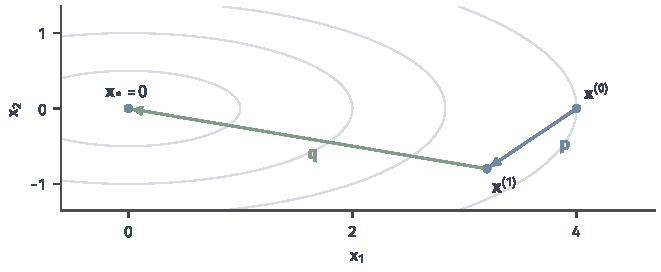
\includegraphics[width=112mm]{figures/01-mathematical-preliminaries-upper/02-linear-spaces/matplotlib/comprehension-additions/linear-conjugate-directions.pdf}
  \caption{共轭方向保留已完成的方向优化。目标为$\phi(\bm x)=\tfrac12(x_1^2+4x_2^2)$，
  灰线为等值线；从$(4,0)^\top$先沿$\bm p=(1,1)^\top$精确线搜索至$(3.2,-0.8)^\top$，
  再沿$\bm q=(-4,1)^\top$到达原点，两方向满足$\bm p^\top\bm A\bm q=0$。本图为解析教学示例。}
  \label{fig:vol1-add-linear-conjugate-directions}
\end{figure}

沿当前方向$\bm p_t$把$\phi$看作步长$\alpha$的一元函数
$\phi(\bm x_t+\alpha\bm p_t)$，展开后对$\alpha$求零点（一维最小化）得
\begin{equation}
 \alpha_t=\frac{\bm p_t^\top\bm r_t}{\bm p_t^\top\bm A\bm p_t}.
\end{equation}
分子是当前方向与残差的配对，分母是方向的能量长度。正定性保证分母
$\bm p_t^\top\bm A\bm p_t>0$，步长合法；若分子为零说明该方向已无改进，
不应再沿它移动。步长不是经验调节参数，而是这一一维最小化的唯一解。

\paragraph{残差正交与方向短递推}

\term{共轭梯度法}（conjugate gradient, CG）从$\bm p_0=\bm r_0$开始：
\begin{align}
 \alpha_t&=\frac{\bm r_t^\top\bm r_t}{\bm p_t^\top\bm A\bm p_t},&
 \bm x_{t+1}&=\bm x_t+\alpha_t\bm p_t,\\
 \bm r_{t+1}&=\bm r_t-\alpha_t\bm A\bm p_t,&
 \beta_t&=\frac{\bm r_{t+1}^\top\bm r_{t+1}}{\bm r_t^\top\bm r_t},\\
 \bm p_{t+1}&=\bm r_{t+1}+\beta_t\bm p_t.&
\end{align}
系数由归纳同时保证三件事：非零残差$\bm r_0,\ldots,\bm r_t$彼此正交；
方向$\bm p_0,\ldots,\bm p_t$彼此$\bm A$共轭；前$t+1$个残差与方向都张成
$\mathcal K_{t+1}$。$t=0$由$\bm p_0=\bm r_0$成立。线搜索使新残差与当前方向
正交；对更早的$j<t$，由$\bm A\bm p_j=(\bm r_j-\bm r_{j+1})/\alpha_j$属于
$\mathcal K_{t+1}$，新残差与之正交，故$\bm r_{t+1}\perp\mathcal K_{t+1}$。
只剩与$\bm p_t$共轭一项需要选$\beta_t$：由新旧残差正交得
$(\bm r_{t+1})^\top\bm A\bm p_t=-\lVert\bm r_{t+1}\rVert_2^2/\alpha_t$，
$(\bm p_t)^\top\bm A\bm p_t=\lVert\bm r_t\rVert_2^2/\alpha_t$，
取$\beta_t=\lVert\bm r_{t+1}\rVert_2^2/\lVert\bm r_t\rVert_2^2$后
$\bm p_{t+1}=\bm r_{t+1}+\beta_t\bm p_t$便与$\bm p_t$共轭，归纳闭合。
$\bm r_t^\top\bm r_t$出现在$\alpha_t$分子，正是因为$(\bm p_t)^\top\bm r_t
=\lVert\bm r_t\rVert_2^2$。

\paragraph{PCG的预条件残差}

\term{预条件共轭梯度}（preconditioned CG, PCG）以对称正定$\bm M$配置预条件，
等价变换系统为$\bm L^{-1}\bm A\bm L^{-\top}\bm z=\bm L^{-1}\bm b$（$\bm M=\bm L\bm L^\top$）。
实现时不解变换坐标，而是每步解$\bm M\bm z_t=\bm r_t$，这里的$\bm z_t$是
预处理后的残差而非变换坐标；初始方向也必须同步改为$\bm p_0=\bm z_0$，
不能只替换迭代中的系数。系数同步改变为
$\alpha_t=\bm r_t^\top\bm z_t/(\bm p_t^\top\bm A\bm p_t)$，
$\beta_t=\bm z_{t+1}^\top\bm r_{t+1}/(\bm z_t^\top\bm r_t)$，
$\bm p_{t+1}=\bm z_{t+1}+\beta_t\bm p_t$。直接把一般非对称左预条件矩阵当作
欧氏对称矩阵是不对的，非对称预条件器不能继承CG的正分母与能量论证。

正定性保证非零方向的$\bm p_t^\top\bm A\bm p_t>0$，分母合法。新残差为零即停止，
不再做含零分母的更新。各次方向更新保证$\bm x_k-\bm x_0\in\mathcal K_k$，
残差与$\mathcal K_k$正交正是该子空间内极小化的一阶条件，正定性又使其充分。
非零共轭方向必线性无关，因此精确算术下至多$d$步得零残差；有限精度下正交性
受损，不能把有限步结论当作实现保证，实际步数与停滞由后续章节说明。
可复算小例子：$\bm A=\operatorname{diag}(1,2)$、$\bm b=(1,1)^\top$、零初值。
第一步$\alpha_0=2/3$得$\bm x^{(1)}=(2/3,2/3)^\top$、
$\bm r^{(1)}=(1/3,-1/3)^\top$，$\beta_0=1/9$给
$\bm p^{(1)}=(4/9,-2/9)^\top$；第二步$\alpha_1=3/4$得
$\bm x^{(2)}=(1,1/2)^\top$，残差恰为零。

每步一次矩阵作用$\bm A\bm p_t$、若干内积（$\bm r_t^\top\bm r_t$、
$\bm p_t^\top\bm A\bm p_t$）与向量更新（$\bm x_{t+1}$、$\bm r_{t+1}$、$\bm p_{t+1}$），
额外存储$O(d)$个向量（当前解、残差、方向；PCG再加预处理残差$\bm z_t$），
不需要形成$\bm A^{-1}$或任何稠密因子。预条件作用、
内积与辅助求解$\bm M\bm z_t=\bm r_t$都计入每步成本；矩阵作用本身按$\bm A$的
非零结构计，稠密与稀疏差别显著。

\subsubsection{MINRES}

\paragraph{对称不定系统与残差目标}

矩阵仍实对称但不正定时，能量范数$\lVert\cdot\rVert_{\bm A}$与正分母失效，
CG的能量最小化论证不能沿用。\term{MINRES}（minimum residual）改在
$\mathcal K_k$中直接最小化原方程残差$\lVert\bm A\bm x-\bm b\rVert_2$，
不要求$\bm A$正定；对称不定性本身不导致不可解，只是不能继续使用CG的
正分母或能量范数论证。

沿用Lanczos短递推构造正交基$\bm V_k$，使
$\bm A\bm V_k=\bm V_{k+1}\bm T_k$，$\bm T_k$为对称三对角（对称使Hessenberg的
次对角与上对角相等，非对角非零项只剩相邻两条）。大系统被压成
逐步更新的小型三对角问题，短递推只需相邻三个向量、不需保存全部基；有限精度下
正交性逐渐损失，必要时重正交化会增加存储与计算。

候选$\bm x=\bm x_0+\bm V_k\bm y$的残差写成$\bm V_{k+1}(\beta\bm e_1-\bm T_k\bm y)$，
其中$\beta=\lVert\bm r_0\rVert_2$；由于$\bm V_{k+1}$列正交，问题化为
\begin{equation}
 \min_{\bm y}\lVert\beta\bm e_1-\bm T_k\bm y\rVert_2.
\end{equation}
这个小型最小二乘用上文的小型QR求解，三对角边界每次只更新一个角，
用Givens旋转逐步完成，无需解大的正规方程。

求得小问题系数$\bm y$后，由$\bm x_k=\bm x_0+\bm V_k\bm y$
恢复解向量；随$\bm V_k$逐列增长，$\bm y$与解都可递推更新，不必每步从头重组。
实现上通常不直接保存$\bm V_k$乘以完整$\bm y$，而是用递推形式更新解向量；
这与CG只保留几个向量不同，MINRES的三对角短递推保留基的投影关系，
恢复路径同样只依赖相邻几列。

预条件仍要求对称正定$\bm M$；投影在$\bm M$内积下进行，
解释的是$\bm M^{-1/2}$尺度下的残差，停止时仍须回到原始残差$\bm b-\bm A\bm x$
核验，不能把变换后残差当作原方程误差。对称不定$\bm A$配上对称正定
（SPD, symmetric positive definite）预条件后，短递推与
三对角结构保持；非对称$\bm M$会破坏三对角对称关系，不满足MINRES前提。

MINRES可扩展到对称奇异相容系统的最小二乘任务，
但一般不保证给出最小欧氏范数代表；它在核方向上的取值仍可能携带自由分量，
选解需另核，MINRES-QLP等变体（专门约束到零空间正交补）不在本节展开。
奇异系统须先判相容（6.2.1），不相容时残差最小化归后续最小二乘任务。

每步一次矩阵作用加少量向量更新，三对角短递推存储与$k$
无关（只需相邻几个向量）；停止以重算的真实原残差$\bm b-\bm A\bm x_k$核验，
递推估计残差在有限精度下可能分离。若 Lanczos 提前出现零余量，说明空间已不变，
应在当前小问题内取残差极小并停止，不对零向量归一化。

\subsubsection{GMRES}
\label{sec:ch06-gmres}

\paragraph{一般系统与Krylov残差目标}

对可逆的一般方阵（无对称性要求），\term{广义最小残差法}（generalized
minimal residual, GMRES）选择
\begin{equation}
 \bm x_k=\argmin_{\bm x\in\bm x_0+\mathcal K_k(\bm A,\bm r_0)}
 \lVert\bm b-\bm A\bm x\rVert_2.
\end{equation}
它放宽的是对称正定要求，不是完全取消结构条件：这里假设$\bm A$可逆；
方法也能用于其他方阵，但其解集与终止结论要另核。

令$\gamma=\lVert\bm r_0\rVert_2>0$，
$\bm v_1=\bm r_0/\gamma$。Arnoldi过程建立正交基$\bm V_k$，满足
$\bm A\bm V_k=\bm V_{k+1}\overline{\bm H}_k$，$\overline{\bm H}_k$为
$(k+1)\times k$上Hessenberg小矩阵。候选$\bm x=\bm x_0+\bm V_k\bm y$的残差为
$\bm V_{k+1}(\gamma\bm e_1-\overline{\bm H}_k\bm y)$，因$\bm V_{k+1}$列正交，
只需解小型最小二乘$\min_{\bm y}\lVert\gamma\bm e_1-\overline{\bm H}_k\bm y\rVert_2$。

小型问题用Givens旋转逐步更新小型QR（见上文Givens旋转），每步只消去
新进入的一行，最后由$\bm x_k=\bm x_0+\bm V_k\bm y$恢复。若第$k$步剩余
长度为零，关系改为$\bm A\bm V_k=\bm V_k\bm H_k$，小问题相应使用
$k\times k$矩阵$\bm H_k$，无需构造不存在的新基向量。可复算小例子：
$\bm A=[1\ 1;0\ 2]$、$\bm b=(0,1)^\top$、零初值。第一步候选$(0,t)^\top$，
残差$(-t,1-2t)^\top$，最小化$t^2+(1-2t)^2$得$t=2/5$，残差范数
$1/\sqrt5$；第二步搜索空间已是$\mathbb R^2$，得精确解$(-1/2,1/2)^\top$。

左预条件$\bm M^{-1}\bm A\bm x=\bm M^{-1}\bm b$最小化
$\lVert\bm M^{-1}(\bm b-\bm A\bm x)\rVert_2$，求解的是变换后残差；
右预条件$\bm A\bm M^{-1}\bm z=\bm b$最小化原系统残差$\lVert\bm b-\bm A\bm x\rVert_2$，
却需把每个搜索方向经$\bm M^{-1}$映回输入。停止时必须说明核验的是哪一个残差，
不能把变换后残差直接当作原方程误差；两种预条件改变的最小化口径不同，结论不可互替。

\paragraph{扩基存储与重启}

第$k$步除一次矩阵作用外，还要把$\bm A\bm v_k$与$k$个基向量逐一做内积正交化，
成本$O(kd)$，基存储$O(kd)$，每次矩阵作用另计；随$k$增长存储线性上升。
\term{重启GMRES}（restarted GMRES, GMRES($m$)）每隔固定$m$步丢弃旧基并从当前
残差重新开始，以把存储压回$O(md)$；代价是放弃已积累的搜索方向。

重启放弃了旧搜索空间中的方向；精确算术下每轮内残差范数
仍不增加（子空间内取最小），但跨轮可能停滞在某一水平，而且不再保证至多$d$步
终止的精确算术保证（旧方向已被丢弃）。何时重启、
重启后是否换预条件，属于策略选择，本节只指出信息损失这一边界；停滞时应改换
预条件或重启参数，而非盲目增加轮次。

一般可逆矩阵在精确算术中至多$d$步终止；若Arnoldi剩余向量提前为零，
当前空间已不变，且可逆性保证精确解已可在$\bm x_0+\mathcal K_k$中取得，
应结束小问题而非继续除以零。停止以重算的真实残差为准，递推残差是否
可信还要结合条件数与后向误差（后续章节）判断。

\subsubsection{BiCGSTAB}

\paragraph{长递推存储与短递推需求}

GMRES的Arnoldi基随步数增长，存储$O(kd)$；
非对称方阵又没有对称三对角的Lanczos短递推（非对称不具备三对角结构）。
\term{BiCGSTAB}（biconjugate gradient stabilized）以两条短递推
换取固定存储，辅助向量数量与每步成本独立于$k$，代价是放弃GMRES的逐步残差
单调最小化保证。

它引入一对互正交的辅助（影子）残差$\tilde{\bm r}$与
双共轭方向，要求$\tilde{\bm r}^\top\bm p_j=0$的双正交条件，不要求欧氏意义下的
A共轭，因而不继承CG的能量论证（没有正定内积保证方向互不干扰）。双共轭条件在
双边（原残差与影子残差）上建立，而非在单一欧氏内积下；影子序列由$\tilde{\bm r}_0$
与转置矩阵$\bm A^\top$生成，与原序列对偶。

双共轭梯度（BiCG）先给出基础校正$\alpha\bm p$，
但其中间残差可能振荡（非正定内积下方向无法保证单调改善）；BiCGSTAB不直接沿用
振荡序列，而在每步基础校正后构造一个局部平稳校正（再沿新方向做一次小残差极小化）
把振荡压平，两个阶段分开。

每步分两个阶段，各一次矩阵作用，实现为固定几个向量的递推，不保存Krylov基矩阵。
第一阶段（BiCG基础校正）：先记$\rho=\tilde{\bm r}^\top\bm r$，
由上一步的$\rho_{\rm prev}$、$\alpha$、$\omega$合成
$\beta=(\rho/\rho_{\rm prev})(\alpha/\omega)$，更新方向
\begin{equation}
 \bm p\leftarrow \bm r+\beta(\bm p-\omega\bm A\bm p),
\end{equation}
再取基础步长
\begin{equation}
 \alpha=\frac{\rho}{\tilde{\bm r}^\top\bm A\bm p},
\end{equation}
把$\alpha\bm p$加到解上，并得中间残差
\begin{equation}
 \bm s=\bm r-\alpha\bm A\bm p.
\end{equation}
第二阶段（局部平稳校正）：在$\bm s$附近沿$\bm A\bm s$方向极小化
$\lVert\bm s-\omega\bm A\bm s\rVert^2$，对$\omega$求零值得
\begin{equation}
 \omega=\frac{\bm s^\top\bm s}{\bm s^\top\bm A\bm s}.
\end{equation}
随后完成本步更新
\begin{equation}
 \bm x\leftarrow\bm x+\alpha\bm p+\omega\bm s,\qquad
 \bm r\leftarrow\bm s-\omega\bm A\bm s,\qquad
 \rho_{\rm prev}\leftarrow\rho,
\end{equation}
方向$\bm p$进入下一步。$\omega$由局部小残差极小化决定，不是经验参数；
完整收敛性、非单调边界与非对称系统的失败模式留第7章，本节只给出可执行更新。

预条件作用在每步辅助求解处插入（解$\bm M\bm z=\bm r$），位置与PCG类似，
但BiCGSTAB本身不要求对称预条件（非对称系统配一般预条件即可）；预条件器改变的是
双正交序列的尺度，不改变方法的非对称性质。

递推有两个关键分母：第一阶段$\alpha$的双共轭分母$\tilde{\bm r}^\top\bm A\bm p$，
第二阶段$\omega$的平稳校正分母$\bm s^\top\bm A\bm s$；任一为零即breakdown，
此时该方向序列无法继续，不能强行代入；近失效（分母极小）
会放大数值误差，应停止并改换方法（如重启GMRES），而非硬除。分母为零属于精确
算术下的结构失效，不是单纯精度问题。

每步约两次矩阵作用与少量内积，不保存Krylov基矩阵，存储为固定个数的向量。
BiCGSTAB不保证残差单调下降（中间可能回升），也没有至多$d$步终止的简单陈述；
结果以重算的真实原残差$\bm b-\bm A\bm x$核验，适用性与失败模式（breakdown、
振荡停滞）归后续章节说明。

\subsection{方法选择与结果核验}

先核验结构判据再选方法：
\begin{enumerate}
 \item 对称正定：优先 Cholesky 或 CG。
 \item 对称不定：MINRES。
 \item 一般方阵（无对称/正定要求，且可逆）：LU 或 GMRES。
 \item 非对称非正定：GMRES 或 BiCGSTAB。
 \item 只能调用$\bm v\mapsto\bm A\bm v$（黑箱）：选 Krylov 方法。
 \item 多右端且矩阵固定：优先复用同一次分解。
\end{enumerate}
对称、正定、稀疏、带状等结构必须先由矩阵本身核验，不能凭方法名称选方法；
目标精度（机器精度级高精度还是宽容限近似）也直接决定直接法与迭代法的取舍：
高精度小系统直接法一步到位，大系统宽容限则迭代法更省。

同任务比较总账：直接法的一次性建立（分解$O(d^3)$）、迭代法的每步成本（矩阵作用
$O(\text{非零元})$）、预条件的辅助求解、存储，以及多右端摊还。不单独按维数或
稀疏性宣布某类方法更快——便宜预条件可能需要更多迭代，贵预条件可能减少步数，
二者相乘（建立$+$每步$\times$步数）才是比较口径。矩阵可整体获得且要求高精度时
直接法核验直接；只能提供矩阵作用或规模极大时迭代法可行，但须把预条件构造计入
总账。

停止一律以原系统残差$\bm b-\bm A\bm x$（按右端或尺度归一）为准，不使用
预条件变换后残差代替；残差小不等于参数准确。解出后回代核验，并复核所选
方法的前提（可逆、正定、非零对角、分母非零）是否满足。条件数、误差放大
与收敛速度由后续扰动与收敛章节报告，本节不提前给阈值。

\section{最小二乘：近似求解}
\label{sec:ls-least-squares}
\label{sec:linear-algebra-residual-systems}
\label{sec:linear-algebra-projection-least-squares}
\label{sec:matrix-analysis-inverse-input-selection}

第~\ref{sec:ls-exact-linear-equations}节要求$\bm A\bm x=\bm b$精确成立，相容性不满足时方程无解。
观测总有误差，方程数也常多于未知数，此时不应再寻找不存在的精确解，而要在所有输入中挑选
使输出误差最小的一个。本节把“误差最小”写成可计算的平方残差目标，分别讨论普通、加权和
正则化三种目标的存在性、唯一性与选解，再给出正规方程、QR、SVD与迭代四类求解路径，
最后说明怎样按矩阵形状、数值尺度和停止准则选择方法并核验结果。灵敏度与收敛速度属于
后续扰动分析与迭代收敛章节，本节只回答目标是什么、解是否存在、怎样更新与核验。

\subsection{残差与目标}
\label{sec:ls-least-squares-objective}

给定$\bm A\in\mathbb R^{m\times d}$和观测$\bm b\in\mathbb R^m$，当不存在$\bm x$使
$\bm A\bm x=\bm b$时，改求使平方输出误差最小的输入：
\begin{equation}
 \min_{\bm x\in\mathbb R^d}\ \lVert\bm A\bm x-\bm b\rVert_2^2.
 \label{eq:linear-algebra-least-squares}
\end{equation}
这一任务称为\term{最小二乘}（least squares）。设计矩阵记号$\bm X\bm w=\bm y$只是同一问题
的回归写法，$\bm X$对应$\bm A$，系数$\bm w$对应$\bm x$，响应$\bm y$对应$\bm b$。
平方误差取欧氏长度的平方，既去掉非负平方根又保持最小点不变，也使目标成为输入的二次函数。

若$\bm b\in\operatorname{range}(\bm A)$，存在输入使残差$\bm r=\bm b-\bm A\bm x$为零，
平方残差的最小值就是$0$；此时最小二乘问题退化为第~\ref{sec:ls-exact-linear-equations}节的
相容精确方程，精确解是最小残差为零的特殊情形，而不是另一种无关的定义。以下讨论集中在
$\bm b$不可达、最小残差严格为正的一般情形。

观测可以同时有若干列。给定$\bm B\in\mathbb R^{m\times n}$，求$\bm X\in\mathbb R^{d\times n}$使
\begin{equation}
 \min_{\bm X}\ \lVert\bm A\bm X-\bm B\rVert_{\mathrm F}^2
 =\sum_{j=1}^n\lVert\bm A\bm x_j-\bm b_j\rVert_2^2,
 \label{eq:ls-multi-right-frobenius}
\end{equation}
其中$\bm b_j$、$\bm x_j$分别是$\bm B$、$\bm X$的第$j$列。Frobenius平方范数把各列残差的
平方长度相加，目标对每一列独立；因此多右端问题就是$n$个同矩阵最小二乘问题并列，分解一次
可以复用于全部列，不存在列间耦合。

不同观测的可靠程度不同，误差代价也不必相同。给定对称正定权重$\bm M\in\mathbb R^{m\times m}$，
\term{加权最小二乘}（weighted least squares）的目标为
\begin{equation}
 \min_{\bm x}\ (\bm A\bm x-\bm b)^\top\bm M(\bm A\bm x-\bm b),
 \label{eq:ls-weighted-objective}
\end{equation}
它等于在$\bm M$内积下度量残差长度，$\bm M$对角元较大的坐标误差被惩罚得更重。权重记录
各输出坐标之间的相对代价，不能与后文惩罚输入幅度的正则化参数混为一谈。若$\bm M$仅半正定，
某些坐标的误差可能被完全忽略，唯一性结论要重新检查，见~\ref{sec:ls-weighted-ls}。

\paragraph{岭回归与一般Tikhonov惩罚}

当矩阵的某些方向几乎不改变输出时，反求的系数会被放大；在数据项之外附加输入幅度的二次惩罚，
得到\term{岭回归}（ridge regression）目标
\begin{equation}
 \min_{\bm x}\ \lVert\bm A\bm x-\bm b\rVert_2^2+\lambda\lVert\bm x\rVert_2^2,
 \qquad \lambda>0.
 \label{eq:ls-ridge-objective}
\end{equation}
更一般地，惩罚可以作用在希望压小的变化量$\bm L\bm x$上，其中$\bm L\in\mathbb R^{p\times d}$
记录这种偏好，得到\term{Tikhonov正则化}（Tikhonov regularization）的一般二次形式
\scite{math-hansen2008regtools}
\begin{equation}
 \min_{\bm x}\ F_\lambda(\bm x)
 =\lVert\bm A\bm x-\bm b\rVert_2^2+\lambda\lVert\bm L\bm x\rVert_2^2,
 \qquad \lambda>0.
 \label{eq:linear-algebra-general-tikhonov}
\end{equation}
$\bm A$记录观测作用，$\bm L$记录要压小的变化，二者行数不必相同；$\bm L=\bm I$时回到岭回归。
惩罚改变的是目标本身，而不是让分解“算得出来”的实现细节：选择$\lambda$是在重新设定任务，
不能仅作为数值技巧解释。

\subsection{存在性、唯一性与选解}
\label{sec:ls-ls-existence}

先在每种目标下回答三个问题：最小点是否存在；若存在，输入是否唯一；不唯一时按什么准则
挑选代表。拟合值$\bm A\bm x$、输入$\bm x$与残差$\bm r$要分别核验，不能互相替代。

\subsubsection{普通最小二乘}
\label{sec:ls-ordinary-ls}

平方残差$\lVert\bm A\bm x-\bm b\rVert_2^2$只通过拟合值$\bm A\bm x$依赖输入：
拟合值遍历列空间$\operatorname{range}(\bm A)$，问题等价于在$\operatorname{range}(\bm A)$中
寻找离$\bm b$最近的点。第~\ref{sec:ls-subspace-nearest-points}节已经证明，有限维子空间中
到给定点的欧氏最近点存在且唯一。

因此最近拟合值$\hat{\bm b}$存在且唯一，与输入是否唯一无关。即便多个输入到达同一个
$\hat{\bm b}$，输出端的选择已经确定。最近点把$\bm b$分解为
$\bm b=\hat{\bm b}+\bm r$，其中$\hat{\bm b}\in\operatorname{range}(\bm A)$，
残差$\bm r$与整个列空间正交。

\paragraph{正交残差与正规方程}

残差与每一列正交，即对任意$\bm x$有$\bm x^\top\bm A^\top\bm r=0$，故
$\bm A^\top\bm r=\bm0$。代入$\bm r=\bm b-\bm A\hat{\bm x}$得到\term{正规方程}
（normal equations）
\begin{equation}
 \bm A^\top(\bm b-\bm A\hat{\bm x})=\bm0,
 \qquad
 \bm A^\top\bm A\hat{\bm x}=\bm A^\top\bm b.
 \label{eq:linear-algebra-normal-equations}
\end{equation}
“正规”来自法向（正交）关系，不是归一化。
图~\ref{fig:ls-least-squares-residual}把这一正交关系画成三维透视：拟合值$\bm A\hat{\bm x}$
落在列空间平面上，残差$\bm r=\bm b-\bm A\hat{\bm x}$与两条列向量都垂直。

\begin{figure}[htbp]
  \centering
  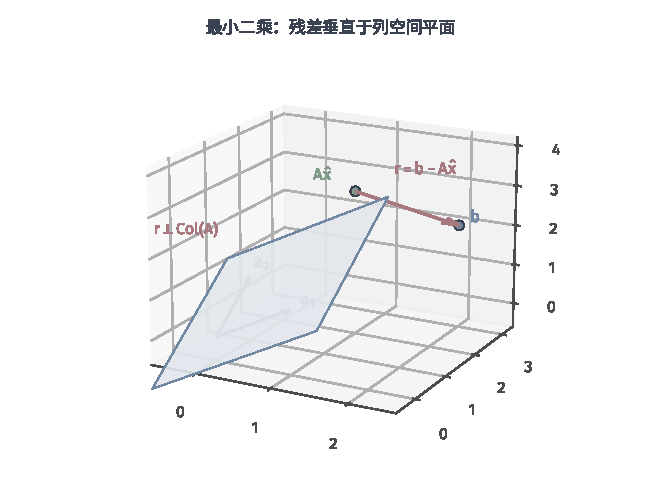
\includegraphics[width=112mm]{figures/01-mathematical-preliminaries-upper/02-linear-spaces/matplotlib/ls-least-squares-residual/ls-least-squares-residual.pdf}
  \caption{列空间平面上的最近点。$\bm A=\left[\begin{smallmatrix}1&0\\0&1\\1&1\end{smallmatrix}\right]$，
  列$\bm a_1=(1,0,1)^\top$、$\bm a_2=(0,1,1)^\top$张成浅蓝平面；$\bm b=(2,3,2)^\top$，
  最近拟合值$\bm A\hat{\bm x}=(1,2,3)^\top$，残差$\bm r=(1,1,-1)^\top$满足
  $\bm r^\top\bm a_1=\bm r^\top\bm a_2=0$。透视教学构造。}
  \label{fig:ls-least-squares-residual}
\end{figure}

正规方程不仅必要，也足以保证全局最小。对任意增量$\bm h$，
\[
 \lVert\bm A(\hat{\bm x}+\bm h)-\bm b\rVert_2^2
 =\lVert\bm A\hat{\bm x}-\bm b\rVert_2^2
 -2\bm h^\top\bm A^\top\bm r+\lVert\bm A\bm h\rVert_2^2.
\]
正规方程使中间项$\bm h^\top\bm A^\top\bm r=\bm h^\top\bm0=0$，剩下非负的
$\lVert\bm A\bm h\rVert_2^2$，故任意移动都不会减小目标。

拟合值唯一不代表输入唯一。若$\hat{\bm x}$是一个解，$\bm z\in\ker\bm A$时
$\bm A(\hat{\bm x}+\bm z)=\hat{\bm b}$不变，所以全部最优输入为
\begin{equation}
 \hat{\bm x}+\ker\bm A.
 \label{eq:ls-all-ordinary-solutions}
\end{equation}
满列秩时$\ker\bm A=\{\bm0\}$，正规矩阵$\bm A^\top\bm A$正定且可逆，唯一输入为
\begin{equation}
 \hat{\bm x}=(\bm A^\top\bm A)^{-1}\bm A^\top\bm b.
 \label{eq:linear-algebra-full-rank-least-squares}
\end{equation}
否则任意零空间增量都不改变目标，输入不唯一。

满列秩只保证系数唯一，不保证系数稳定。贯穿例（设计矩阵~\eqref{eq:linear-algebra-nearly-collinear-design}）
展示两列几乎同向时系数如何被放大。取$\bm c_1=(1,1,1)^\top$、$\bm q=(0,1,-1)^\top$，
两列为$\bm c_1$与$\bm c_1+\varepsilon\bm q$，响应$\bm y=\bm c_1+\delta\bm q$。
正规方程具体为
\[
 \begin{bmatrix}3&3\\3&3+2\varepsilon^2\end{bmatrix}\hat{\bm w}
 =\begin{bmatrix}3\\3+2\varepsilon\delta\end{bmatrix},
\]
系数矩阵行列式为$6\varepsilon^2$。$\varepsilon\neq0$时满列秩，
\begin{equation}
 \hat{\bm w}_\varepsilon
 =\begin{bmatrix}1-\delta/\varepsilon\\\delta/\varepsilon\end{bmatrix},
 \qquad\bm X_\varepsilon\hat{\bm w}_\varepsilon=\bm y,
 \label{eq:linear-algebra-nearly-collinear-least-squares}
\end{equation}
$\varepsilon=0.01$、$\delta=0.1$时系数为$(-9,10)^\top$，残差却为零。
$\varepsilon=0$时两列重合为$\bm c_1$，正交分解$\bm y=\bm c_1+\delta\bm q$的最近输出
为$\bm c_1$，残差为$\delta\bm q$（平方残差$2\delta^2$），全部系数满足$w_1+w_2=1$。
于是矩阵趋于极限时，精确拟合所需的系数发散，而极限矩阵不再能精确拟合：拟合值可以相当
稳定，表示它的两个系数却可能很大。这是近共线几何本身的结果，不是计算机造成的现象。

输入多解时需要额外准则选定代表。要求欧氏范数最小，就是去掉不改变输出的零空间分量：
把$\hat{\bm x}$分解为$(\ker\bm A)^\perp$分量与$\ker\bm A$分量，两项正交，平方范数相加，
最小值只在零空间分量为零时达到。这一选择的显式构造留给伪逆，见~\ref{sec:ls-pseudoinverse}。

\subsubsection{加权最小二乘}
\label{sec:ls-weighted-ls}

加权目标$(\bm A\bm x-\bm b)^\top\bm M(\bm A\bm x-\bm b)$中的$\bm M$对称正定。
它定义输出空间的$\bm M$内积$\langle\bm u,\bm v\rangle_{\bm M}=\bm u^\top\bm M\bm v$，
加权残差在该内积下与列空间正交。

\paragraph{白化后的普通最小二乘}

由~\ref{thm:ls-gram-factor}的配方结论，正定$\bm M$可写成$\bm M=\bm R^\top\bm R$，
其中$\bm R$可逆。令$\tilde{\bm A}=\bm R\bm A$、$\tilde{\bm b}=\bm R\bm b$，则
加权目标等于普通平方残差$\lVert\tilde{\bm A}\bm x-\tilde{\bm b}\rVert_2^2$。
这一步常称\term{白化}（whitening）：先把各坐标误差变换到同一欧氏尺度，再回到已证的
普通问题。正交条件给出加权正规方程
\begin{equation}
 \bm A^\top\bm M(\bm b-\bm A\hat{\bm x})=\bm0,
 \qquad
 \bm A^\top\bm M\bm A\,\hat{\bm x}=\bm A^\top\bm M\bm b.
 \label{eq:linear-algebra-weighted-normal-equations}
\end{equation}

白化后的最近点存在唯一，故加权拟合值$\bm A\hat{\bm x}$存在。满列秩时
$\bm A^\top\bm M\bm A$正定，输入唯一；欠定或列相关时，输入仍沿$\ker\bm A$模糊，
与普通情形同理。

若$\bm M$仅半正定，它可能忽略非零残差：例如$\bm A=\bm I$、$\bm M=\operatorname{diag}(1,0)$
时第二个拟合坐标不受目标约束，任意取值都不改变代价。被$\bm M$消去的输出方向上，
拟合值本身不再唯一，不能直接沿用正定权重的结论。

半正定$\bm M$仍给出半内积，目标在有限维输入上连续；在受约束的方向范围内取到下界，
最小点存在；不可辨认方向构成解集的仿射纤维，可在其中另取欧氏范数最小的代表。
这种选择不恢复被权重消去的信息，只是在等价解中挑一个规范代表。

多右端时若各列共用同一个$\bm M$，各列仍然独立。若不同输出坐标或不同右端列需要不同权重，
把矩阵按列向量化后，权重作用在拉长的残差向量上，列间通过权重矩阵耦合，不能再逐列独立求解。

\subsubsection{正则化最小二乘}
\label{sec:ls-regularized-ls}

一般Tikhonov目标$F_\lambda(\bm x)=\lVert\bm A\bm x-\bm b\rVert_2^2+\lambda\lVert\bm L\bm x\rVert_2^2$
同时衡量数据拟合与惩罚量。两项都非负，$\lambda>0$平衡二者；这不是普通最小二乘的近似，
而是另一个目标。

\paragraph{二次增量与正规算子}

在$\hat{\bm x}$处沿$\bm h$移动，数据项增量为
$\lVert\bm A\bm h\rVert_2^2-2\bm h^\top\bm A^\top(\bm b-\bm A\hat{\bm x})$，
惩罚项增量为$\lambda\lVert\bm L\bm h\rVert_2^2$。一阶项合并为零的条件是
\begin{equation}
 (\bm A^\top\bm A+\lambda\bm L^\top\bm L)\hat{\bm x}=\bm A^\top\bm b.
 \label{eq:ls-tikhonov-normal}
\end{equation}
系数矩阵$\bm A^\top\bm A+\lambda\bm L^\top\bm L$对称，对任意$\bm h$其二次型为
$\lVert\bm A\bm h\rVert_2^2+\lambda\lVert\bm L\bm h\rVert_2^2\geq0$。

二次型为零当且仅当$\bm A\bm h=\bm0$且$\bm L\bm h=\bm0$，即
\begin{equation}
 \ker\bm A\cap\ker\bm L=\{\bm0\}
 \label{eq:linear-algebra-tikhonov-common-nullspace}
\end{equation}
时系数矩阵正定；否则沿公共零空间方向既不改变观测也不改变惩罚，目标对该方向平坦。

正规算子对称，方程有解当且仅当右端$\bm A^\top\bm b$与其零空间正交：对公共零空间中的$\bm z$，
$\bm z^\top\bm A^\top\bm b=(\bm A\bm z)^\top\bm b=0$恒成立，故相容性自动满足，最小点存在。

$\lambda>0$时，若公共零空间为零，系数矩阵正定，增量
$\lVert\bm A\bm h\rVert_2^2+\lambda\lVert\bm L\bm h\rVert_2^2$对$\bm h\neq\bm0$严格为正，
最小点唯一。公共零空间非零时，所有最小点仍相差该空间中的向量，可另取范数最小代表，
正则化并不恢复被两者共同消去的方向。$\bm L=\bm I$时公共零空间自动为零，岭回归因而总有
唯一解；差分惩罚则未必，例如$\bm A=\bm L=[\,1\ -1\,]$时常量方向$(1,1)^\top$
仍在公共零空间中，无论$\lambda$多大都不能确定两个值的共同水平。

$\lambda=0$时目标退回普通最小二乘，唯一性由$\ker\bm A$决定；$\lambda$从正降到零是目标的
连续改变，不是同一问题的参数微调。$\lambda\to\infty$时解趋于$\ker\bm L$中的最小二乘代表，
两端的极限行为在参数选择处再用。

\subsection{直接法}
\label{sec:ls-direct-methods-ls}

直接法把系数矩阵化成可回代的因子。三种路径对应三种矩阵处境：满列秩且规模适中时形成
正规方程；要避免Gram矩阵损失尺度时用QR；秩未知、矩形且需要四个子空间时用SVD。

\subsubsection{正规方程法}
\label{sec:ls-normal-equations-method}

由~\eqref{eq:linear-algebra-normal-equations}，最小二乘解满足对称正规方程
$\bm A^\top\bm A\hat{\bm x}=\bm A^\top\bm b$。这是一个$d$阶对称方阵方程，第~\ref{sec:ls-direct-methods}节
建立的对称正定求解工具可以直接套用。

$\bm A$满列秩时$\bm A^\top\bm A$正定：$\bm x^\top\bm A^\top\bm A\bm x=\lVert\bm A\bm x\rVert_2^2$，
且$\bm A\bm x=0$只在$\bm x=0$时成立。因而正规方程有唯一解，不需要额外选解准则。

对正定$\bm A^\top\bm A$作Cholesky分解$\bm L\bm L^\top$，依次前代求$\bm L\bm z=\bm A^\top\bm b$、
回代求$\bm L^\top\hat{\bm x}=\bm z$，复用第~\ref{sec:ls-direct-methods}节的对称分解流程，
不另立新算法。加权目标对$\bm A^\top\bm M\bm A$、正则化目标对
$\bm A^\top\bm A+\lambda\bm L^\top\bm L$作同样分解，后者正定性由公共零空间条件保证。

稠密矩阵先计算$\bm A^\top\bm A$（约$md^2$次乘法），再作$d^3/3$量级的Cholesky；
多个右端复用同一分解。这一方法只需要矩阵整体可访问，适合小型满列秩问题。

形成$\bm A^\top\bm A$把小的奇异方向平方：接近零的方向被压得更小，浮点中可能直接与零
不可区分。正规方程法只在列之间明显分离、$\bm A^\top\bm A$正定余量充足时可靠；
秩亏或近秩亏时，唯一性本身已经不成立，分解成功也不给出正确选解。条件数放大的定量估计
属于扰动分析，此处只记录这一尺度损失现象。

\subsubsection{QR分解}
\label{sec:ls-qr-method}
\label{sec:linear-algebra-direct-residual}

对$\bm A$作QR分解的构造见第~\ref{sec:ls-orthogonalization-qr}节。正交矩阵保持欧氏长度，
故$\lVert\bm A\bm x-\bm b\rVert_2^2=\lVert\bm Q^\top\bm A\bm x-\bm Q^\top\bm b\rVert_2^2$，
最小点不变。这是QR适合最小二乘的根本原因：只改坐标，不改长度。

瘦QR给出$\bm A=\bm Q\bm R$，$\bm Q$列正交，$\bm R$为上三角。记
$\bm Q^\top\bm b=(\bm c_1,\bm c_2)^\top$、$\bm Q=(\bm Q_1,\bm Q_2)$，则
\[
 \lVert\bm Q\bm R\bm x-\bm b\rVert_2^2
 =\lVert\bm R\bm x-\bm c_1\rVert_2^2+\lVert\bm c_2\rVert_2^2.
\]
$\bm c_2$不依赖$\bm x$，是固定残差；可调部分只由上三角方程决定。

满列秩时$\bm R$满秩，$\bm R\hat{\bm x}=\bm c_1$上三角可直接回代，目标最小值就是
$\lVert\bm c_2\rVert_2^2$。QR不显式形成$\bm A^\top\bm A$，避免正规方程的平方尺度损失，
代价是分解本身的运算量高于Cholesky。

欠定（$m<d$）相容时，QR配合行空间表示可给出最小范数解：解落在$\operatorname{range}(\bm A^\top)$，
正交于$\ker\bm A$。完整的最小范数构造在伪逆处给出，此处只说明QR同样服务于这一选解。

带列主元的QR按接近独立的顺序排列列，使接近零的对角元集中到尾部，从而暴露数值秩。
秩的阈值与噪声尺度有关，见~\ref{sec:ls-method-selection}。

秩亏时取前$r$个主元列回代得到一个基本解，自由方向补零；它是一个合法最优解，但未必
最小范数。核验时同时检查输出残差$\bm b-\bm A\hat{\bm x}$与最优性残差
$\bm A^\top(\bm b-\bm A\hat{\bm x})$，并在需要最小范数时核对$\hat{\bm x}$是否正交于
$\ker\bm A$。

\subsubsection{SVD分解}
\label{sec:ls-svd}

QR只处理满列秩或秩揭示的情形；秩未知、矩形矩阵需要同时给出非零方向、零方向、四个子空间
和稳定选解时，使用奇异值分解。它的存在性不能假设：下面先用实对称谱引理从单位球极值
直接构造，这也是全卷首次建立谱定理，后续球面极值、低秩逼近与矩阵函数都复用这一结论。

对任意$\bm A\in\mathbb R^{m\times d}$，希望找到两组正交方向，使$\bm A$在其间只作独立
伸缩。这需要先证明\term{谱定理}（spectral theorem）：对称矩阵能在正交基下对角化。

\begin{lemma}[实对称谱引理]
\label{thm:ls-real-symmetric-spectral}
\label{thm:matrix-analysis-symmetric-spectral-theorem}
\label{sec:ch06-triangular-spectrum}
设$\bm S\in\mathbb R^{d\times d}$满足$\bm S=\bm S^\top$。存在正交矩阵$\bm Q$与实对角
$\Lambda=\operatorname{diag}(\lambda_1,\dots,\lambda_d)$，使
\begin{equation}
 \bm S=\bm Q\Lambda\bm Q^\top,
 \qquad \bm S\bm q_i=\lambda_i\bm q_i.
 \label{eq:matrix-analysis-symmetric-eigendecomposition}
\end{equation}
对任意$\bm x=\sum_i c_i\bm q_i$，二次型展开为
\begin{equation}
 \bm x^\top\bm S\bm x=\sum_{i=1}^d\lambda_i c_i^2.
 \label{eq:matrix-analysis-quadratic-spectral-form}
\end{equation}
\end{lemma}

\begin{proof}
单位球面$\{\bm x:\lVert\bm x\rVert_2=1\}$是$\mathbb R^d$中的闭有界集，二次型
$q(\bm x)=\bm x^\top\bm S\bm x$连续，由~\ref{thm:ls-extreme-value}在球上取到最大值
$\lambda_1$，记最大点为$\bm q_1$，$\lVert\bm q_1\rVert_2=1$。实对称保证
$\lambda_1=\bm q_1^\top\bm S\bm q_1$是实数。

任取与$\bm q_1$正交的$\bm h$，实数$t$很小时$\bm q_1+t\bm h$归一化后仍在球上，
故其二次型不超过$\lambda_1$倍范数平方。展开：
\[
 \lambda_1+2t\bm h^\top\bm S\bm q_1+t^2\bm h^\top\bm S\bm h
 \leq\lambda_1(1+t^2\lVert\bm h\rVert_2^2).
\]
两边减去$\lambda_1$，$t$的一阶项$2t\bm h^\top\bm S\bm q_1$必须对正负$t$同时不破坏
不等式，因而只能为零，即$\bm h^\top\bm S\bm q_1=0$。对所有$\bm h\perp\bm q_1$成立，
说明$\bm S\bm q_1$没有正交分量，只能平行于$\bm q_1$，即$\bm S\bm q_1=\lambda_1\bm q_1$。
全程只用有限代数增量，不引入复特征多项式。

对$\bm h\perp\bm q_1$，$\bm q_1^\top\bm S\bm h=(\bm S\bm q_1)^\top\bm h
=\lambda_1\bm q_1^\top\bm h=0$，故$\bm S$把$\bm q_1^\perp$映到自身，限制仍是对称矩阵。
在$d-1$维正交补上重复同一极值构造，得到$\bm q_2,\lambda_2$；归纳到一维即得正交列
$\bm q_1,\dots,\bm q_d$与实特征值$\lambda_i$。代入$\bm x=\sum_i c_i\bm q_i$交叉项为零，
便得到谱展开式。这一证明只依赖球的紧性与对称配对，是实情形的完整谱定理；复Hermitian
情形的共轭转置推广在矩阵函数章再给。
\end{proof}

令$\bm S=\bm A^\top\bm A$，它对称且半正定：$\bm x^\top\bm A^\top\bm A\bm x
=\lVert\bm A\bm x\rVert_2^2\geq0$。由谱引理，存在标准正交的$\bm v_i$使
$\bm A^\top\bm A\bm v_i=\lambda_i\bm v_i$，且$\lambda_i\geq0$。记正特征值为
$\sigma_i^2=\lambda_i>0$（$i=1,\dots,r$），$\sigma_i>0$，按降序排列；其余$\bm v_j$满足
$\bm A^\top\bm A\bm v_j=0$，因而$\bm A\bm v_j=0$。

对$\sigma_i>0$定义$\bm u_i=\bm A\bm v_i/\sigma_i$。它们标准正交：
\[
 \bm u_i^\top\bm u_j
 =\frac{\bm v_i^\top\bm A^\top\bm A\bm v_j}{\sigma_i\sigma_j}
 =\frac{\sigma_i^2\delta_{ij}}{\sigma_i\sigma_j}=\delta_{ij}.
\]
且$\bm A\bm v_i=\sigma_i\bm u_i$。

$\bm v_{r+1},\dots,\bm v_d$是$\ker\bm A$的标准正交基；把$\bm u_1,\dots,\bm u_r$扩充为
$\mathbb R^m$的标准正交基，多余方向落在$\operatorname{range}(\bm A)^\perp$。于是
$\bm A$写成秩一矩阵之和
\begin{equation}
 \bm A=\sum_{i=1}^r\sigma_i\bm u_i\bm v_i^\top.
 \label{eq:matrix-analysis-svd-rank-one-sum}
\end{equation}
其中$r=\operatorname{rank}\bm A$，非零奇异值个数就是秩。

\begin{theorem}[SVD的存在与构造]
\label{thm:ls-svd-existence}
对任意$\bm A\in\mathbb R^{m\times d}$，上述构造给出正交$\bm U\in\mathbb R^{m\times m}$、
$\bm V\in\mathbb R^{d\times d}$与对角$\Sigma\in\mathbb R^{m\times d}$，非负对角元
$\sigma_i$使$\bm A=\bm U\Sigma\bm V^\top$。
\end{theorem}

\begin{definition}[奇异值分解]
\label{def:matrix-analysis-svd}
称
\begin{equation}
 \bm A=\bm U\Sigma\bm V^\top
 \label{eq:matrix-analysis-svd}
\end{equation}
为\term{奇异值分解}（singular value decomposition, SVD），非负对角元$\sigma_i$为
\term{奇异值}（singular value），$\bm u_i$、$\bm v_i$分别为左、右\term{奇异向量}
（singular vector）。
\end{definition}

图~\ref{fig:ls-svd-construction}把这一构造拆成三步：先形成对称$\bm A^\top\bm A$，
再由谱引理正交对角化取特征值，最后开方得奇异值、并由$\bm u_i=\bm A\bm v_i/\sigma_i$
得左奇异向量。

\begin{figure*}[htbp]
  \centering
  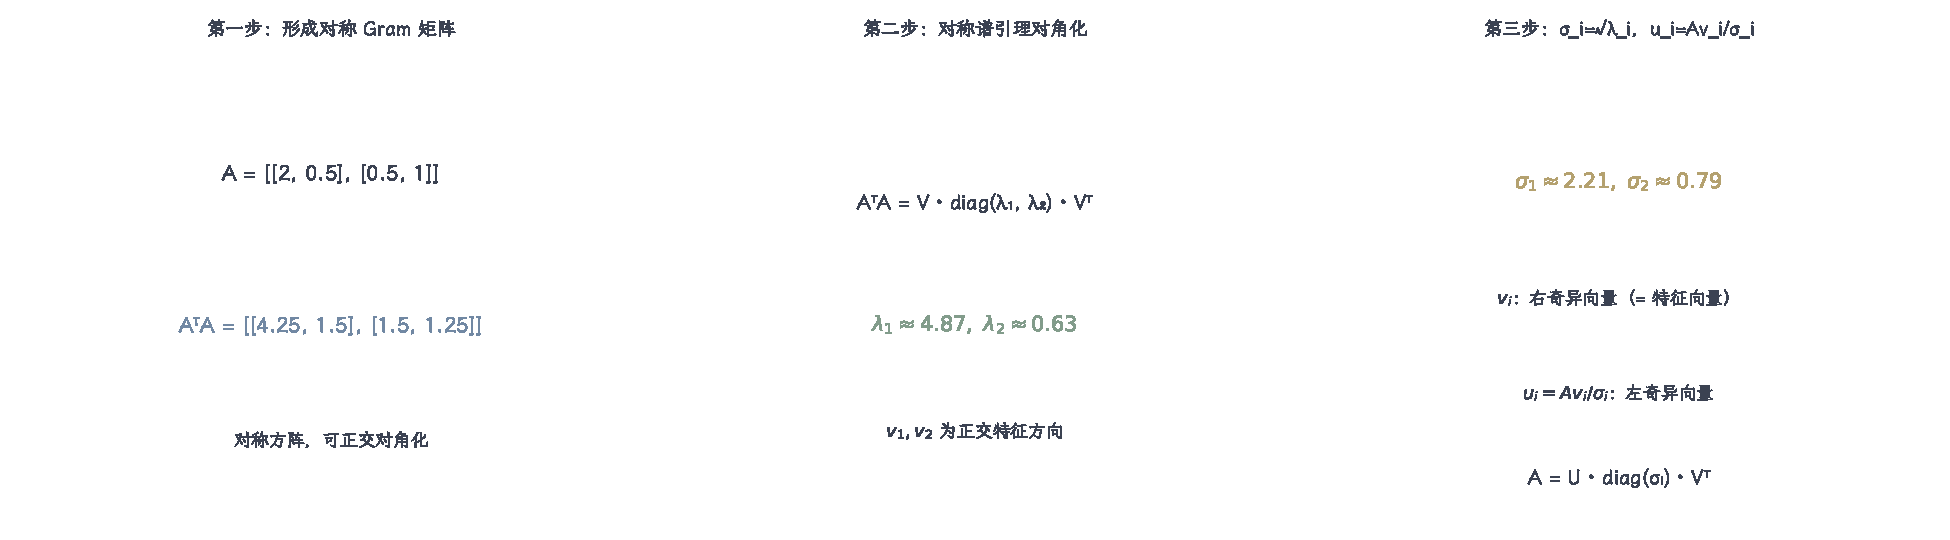
\includegraphics[width=168.998mm]{figures/01-mathematical-preliminaries-upper/02-linear-spaces/matplotlib/ls-svd-construction/ls-svd-construction.pdf}
  \caption{SVD 构造三部曲。以$\bm A=\left[\begin{smallmatrix}2&0.5\\0.5&1\end{smallmatrix}\right]$为例：
  (1)形成$\bm A^\top\bm A=\left[\begin{smallmatrix}4.25&1.5\\1.5&1.25\end{smallmatrix}\right]$；
  (2)对称谱引理对角化，特征值$\lambda_1\approx4.87,\lambda_2\approx0.63$；
  (3)$\sigma_i=\sqrt{\lambda_i}\approx2.21,0.79$，右奇异向量$\bm v_i$即特征向量，
  左奇异向量$\bm u_i=\bm A\bm v_i/\sigma_i$。解析式教学构造。}
  \label{fig:ls-svd-construction}
\end{figure*}

图~\ref{fig:matrix-analysis-svd-geometry}使用二维旋转矩阵
$\bm R(\theta)=
\left[\begin{smallmatrix}\cos\theta&-\sin\theta\\\sin\theta&\cos\theta\end{smallmatrix}\right]$
构造一个左右方向不同的变换，两侧采用相同比例便于比较伸缩量。

\begin{figure*}[htbp]
  \centering
  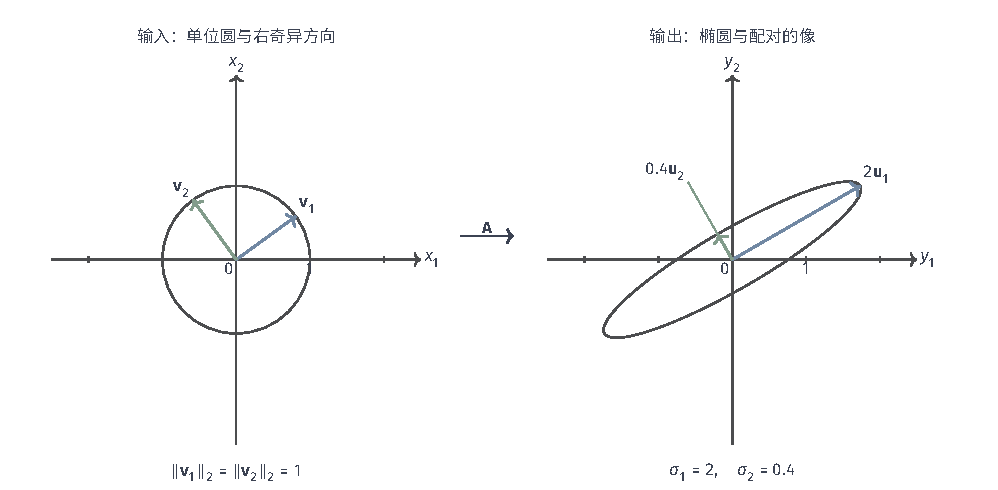
\includegraphics[width=168.998mm]{figures/01-mathematical-preliminaries-upper/02-linear-spaces/tikz/matrix-analysis-svd-geometry/figure.pdf}
  \caption{矩阵$\bm A=\bm R(\pi/6)\operatorname{diag}(2,0.4)\bm R(\pi/5)^\top$
  将单位圆变为椭圆。蓝、绿分别对应两个奇异方向；同色箭头在左侧标出$\bm v_i$，
  在右侧标出其像$\sigma_i\bm u_i$。两侧坐标比例相同。奇异值决定长度变化，左右方向可以不同，
  因而这不是沿特征方向的同空间缩放。图为教学构造。}
  \label{fig:matrix-analysis-svd-geometry}
\end{figure*}

与这一“单位圆变椭圆”的输入侧视角互补，图~\ref{fig:ls-svd-ellipse-action}从行图像与
列图像两侧看最小二乘解：左图两条方程直线交于$\hat{\bm x}=(1,1)^\top$，残差二次型的
水平集是以它为中心的同心椭圆；右图$\bm b$恰落在列空间内，残差为零。

\begin{figure*}[htbp]
  \centering
  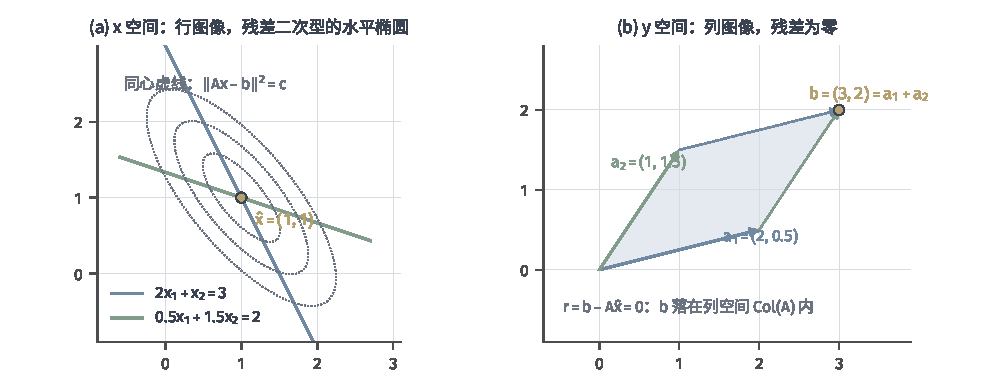
\includegraphics[width=168.998mm]{figures/01-mathematical-preliminaries-upper/02-linear-spaces/matplotlib/ls-svd-ellipse-action/ls-svd-ellipse-action.pdf}
  \caption{最小二乘解的行图像与列图像。$\bm A=\left[\begin{smallmatrix}2&1\\0.5&1.5\end{smallmatrix}\right]$、
  $\bm b=(3,2)^\top$，$\bm A\hat{\bm x}=\bm b$恰有解$\hat{\bm x}=(1,1)^\top$。左：两条方程直线
  交于$\hat{\bm x}$，灰色点线为残差平方$f(\bm x)=\lVert\bm A\bm x-\bm b\rVert_2^2$的水平集，
  中心即交点；右：列$\bm a_1=(2,0.5)^\top$、$\bm a_2=(1,1.5)^\top$张成列空间，
  $\bm b=\bm a_1+\bm a_2$落在其中，残差为零。解析式教学构造。}
  \label{fig:ls-svd-ellipse-action}
\end{figure*}

$\sigma_i$相同时，对应子空间内的任意标准正交旋转仍给出分解，故$\bm U,\bm V$不唯一；
奇异值本身由$\bm A$唯一确定。零奇异值对应的方向不参与伸缩。

数值实现先以Householder双边约化把矩阵变成上双对角形（复用~\ref{sec:ls-orthogonalization-qr}
的反射工具），再用隐式QR位移迭代得到对角元；直接对$\bm A^\top\bm A$求特征值会重蹈
平方尺度损失，故实现始终作用在原矩阵上。

以贯穿例的二维约化看清两个尺度。把设计的输出限制到$\operatorname{span}\{\bm c_1,\bm q\}$，
用$\bm c_1/\sqrt3$、$\bm q/\sqrt2$作正交坐标，再将全部输出统一除以$\sqrt3$，
得到二维表示
\begin{equation}
 \bm X_{\widetilde\varepsilon}
 =\begin{bmatrix}1&1\\0&\widetilde\varepsilon\end{bmatrix},
 \qquad \widetilde\varepsilon=\sqrt{2/3}\,\varepsilon.
 \label{eq:matrix-analysis-nearly-collinear-design}
\end{equation}
这一统一缩放把奇异值除以$\sqrt3$，不改变它们的比值。二维Gram矩阵为
$\bm G_{\widetilde\varepsilon}
=\begin{bmatrix}1&1\\1&1+\widetilde\varepsilon^2\end{bmatrix}$，
其两个特征值由二次方程得到
\begin{equation}
 \lambda_\pm
 =\frac{2+\widetilde\varepsilon^2
          \mathbin{\pm}\sqrt{4+\widetilde\varepsilon^4}}{2},
 \label{eq:matrix-analysis-nearly-collinear-gram-eigenvalues}
\end{equation}
对$\widetilde\varepsilon>0$，$\sigma_\pm=\sqrt{\lambda_\pm}$；
$\widetilde\varepsilon\to0$时$\sigma_{\max}\to\sqrt2$、
$\sigma_{\min}\sim\widetilde\varepsilon/\sqrt2$。大方向近似为两个系数一起变化，
小方向近似为两个系数相消。这一推导只用于理解谱；为计算小奇异值不应显式形成Gram矩阵，
也不宜用相近两数相减求$\lambda_-$，定量原因留给扰动章节。

完整SVD给出$\bm U,\bm V$全正交基；只需要前$k$个奇异方向时可计算薄分解，省去尾部。
稠密完整分解的运算量高于QR，但其明示全部奇异值、四个子空间与最小二乘选解，是秩未知
矩形矩阵的通用工具。

\subsubsection{伪逆与全部最优解}
\label{sec:ls-pseudoinverse}

先看一个欠定小例。$\bm A=[2\ 0]$把$(x_1,x_2)^\top$映成$2x_1$，取$\bm b=(3)$：
方程$2x_1=3$的全部解为$(3/2,t)^\top$，$t$任意，输出只由$x_1$决定。
范数平方$(3/2)^2+t^2$在$t=0$时最小，代表点$(3/2,0)^\top$——它自动落在
$\operatorname{range}(\bm A^\top)$方向上、把零空间分量压为零。伪逆就是把“全部解中
范数最小者”写成一个矩阵的规则：本例$\bm A^\dagger=(1/2,0)^\top$，
$\bm A^\dagger\bm b=(3/2,0)^\top$。下面用SVD把这一规则推广到任意秩。

在$\bm v_i$方向上$\bm A$以$\sigma_i$伸缩到$\bm u_i$，反向自然除以$\sigma_i$：
$\bm u_i\mapsto\bm v_i/\sigma_i$。把$\bm b$按$\bm u_i$展开，可恢复分量
$(\bm u_i^\top\bm b)/\sigma_i$配给$\bm v_i$；落在$\operatorname{range}(\bm A)^\perp$的
分量没有原像，直接丢弃；零方向$\bm v_{r+1},\dots$上$\bm A$没有输出，反向不定义。
小$\sigma_i$在正向作用中压缩，反求时把该分量放大，这是伪逆对弱方向敏感的来源，定量
放大分析属扰动章节。

\begin{definition}[Moore--Penrose伪逆]
\label{def:matrix-analysis-pseudoinverse}
在两端标准内积下，\term{Moore--Penrose伪逆}（Moore--Penrose pseudoinverse）先把
输出正交投影到$\operatorname{range}(\bm A)$，再在$(\ker\bm A)^\perp$上反演：
\[
 \bm A^\dagger=(\bm A|_{(\ker\bm A)^\perp})^{-1}P_{\operatorname{range}(\bm A)}.
\]
用~\ref{thm:ls-svd-existence}的SVD写出即
\begin{equation}
 \bm A^\dagger=\sum_{i=1}^r\frac{1}{\sigma_i}\bm v_i\bm u_i^\top,
 \label{eq:matrix-analysis-pseudoinverse}
\end{equation}
它在$\operatorname{range}(\bm A)^\perp$上取零；$\bm A=\bm0$时定义$\bm A^\dagger=\bm0$。
普通逆是伪逆在可逆方阵上的特殊情形。
\end{definition}

\begin{theorem}[最小二乘与最小范数]
\label{thm:matrix-analysis-pseudoinverse-minimum-norm}
给定$\bm A\in\mathbb R^{m\times d}$和$\bm b\in\mathbb R^m$，全部最小二乘解为
$\bm A^\dagger\bm b+\ker\bm A$，其中$\bm A^\dagger\bm b$是唯一的最小欧氏范数解；
方程相容时它就是全部精确解中的最小范数者。
\begin{proof}
记$P_R$为到$\operatorname{range}\bm A$的正交投影。把
$\bm b=P_R\bm b+\bm b_\perp$（$\bm b_\perp\perp\operatorname{range}\bm A$）、
$\bm x=\bm x_\perp+\bm x_N$（$\bm x_N\in\ker\bm A$）正交分解，则
\[
 \lVert\bm A\bm x-\bm b\rVert_2^2
 =\lVert\bm A\bm x_\perp-P_R\bm b\rVert_2^2+\lVert\bm b_\perp\rVert_2^2.
\]
第二项不能由输入改变；第一项在且仅在$\bm x_\perp$等于投影反演
$(\bm A|_{(\ker\bm A)^\perp})^{-1}P_R\bm b$，也就是$\bm A^\dagger\bm b$时为零。
故全部最优输入为$\bm A^\dagger\bm b+\bm x_N$。两项正交，
$\lVert\bm x\rVert_2^2=\lVert\bm A^\dagger\bm b\rVert_2^2+\lVert\bm x_N\rVert_2^2$，
最小值仅在$\bm x_N=0$时达到。相容时$\bm b_\perp=0$，同一证明适用。
\end{proof}
\end{theorem}

\paragraph{Penrose条件的逐项验证}

由SVD和式直接相乘逐项核对四条：
\begin{enumerate}
 \item $\bm A\bm A^\dagger\bm A=\bm A$；
 \item $\bm A^\dagger\bm A\bm A^\dagger=\bm A^\dagger$；
 \item $(\bm A\bm A^\dagger)^\top=\bm A\bm A^\dagger$；
 \item $(\bm A^\dagger\bm A)^\top=\bm A^\dagger\bm A$。
\end{enumerate}
前两项保证在可反演部分上一致，后两条说明
$\bm A\bm A^\dagger$是到$\operatorname{range}(\bm A)$的正交投影、
$\bm A^\dagger\bm A$是到$(\ker\bm A)^\perp$的正交投影。

满足同样四条的矩阵唯一：若$\bm G$也满足，则$\bm A\bm G=P_R$、$\bm G\bm A=P_{(\ker\bm A)^\perp}$，
于是$\bm G=\bm G\bm A\bm G=P_{(\ker\bm A)^\perp}\bm A^\dagger=\bm A^\dagger$。
故伪逆不由SVD写法决定，是矩阵本身的性质。

$\bm A\bm A^\dagger=\sum_i\bm u_i\bm u_i^\top=P_{\operatorname{range}(\bm A)}$，
$\bm A^\dagger\bm A=\sum_i\bm v_i\bm v_i^\top=P_{(\ker\bm A)^\perp}$；
$\operatorname{range}(\bm A^\dagger)=(\ker\bm A)^\perp$，
$\ker(\bm A^\dagger)=\operatorname{range}(\bm A)^\perp$。四个子空间分属输入端与输出端，
与伴随的正交补关系一致。

例如$\bm A=\begin{smallmatrix}1&1\\0&0\end{smallmatrix}$、$\bm b=(2,1)^\top$，
可达输出只有第二坐标为零的$(2,0)^\top$，残差$(0,1)^\top$无法消除；原像直线
$x_1+x_2=2$上平方范数为$2+2t^2$，伪逆选择$t=0$得到$(1,1)^\top$。伪逆没有使
原本无解的方程突然可解，也没有恢复被$\bm A$消去的信息。

\begin{figure*}[htbp]
  \centering
  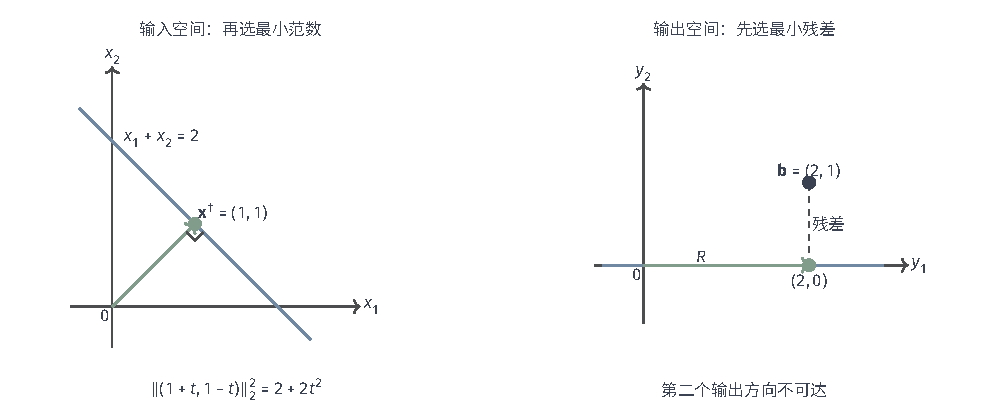
\includegraphics[width=168.998mm]{figures/01-mathematical-preliminaries-upper/02-linear-spaces/tikz/matrix-analysis-pseudoinverse-selections/figure.pdf}
  \caption{伪逆的两次选择。右图先在可达输出中选择离$\bm b=(2,1)^\top$最近的
  $(2,0)^\top$；左图再在整条原像直线$x_1+x_2=2$上选择最靠近原点的$(1,1)^\top$。
  两图属于不同空间，各自等比例绘制。}
  \label{fig:matrix-analysis-pseudoinverse-selections}
\end{figure*}

全部最优输入为
\begin{equation}
 \hat{\bm x}=\bm A^\dagger\bm b+\bm z,
 \qquad \bm z\in\ker\bm A.
 \label{eq:ls-all-pseudoinverse-solutions}
\end{equation}
由证明中的正交分解，$\bm z=0$时范数最小。这就完成了~\ref{sec:ls-ordinary-ls}节
承诺的选解构造。

满列秩时$\bm A^\dagger=(\bm A^\top\bm A)^{-1}\bm A^\top$；满行秩时
$\bm A^\dagger=\bm A^\top(\bm A\bm A^\top)^{-1}$，用于相容欠定系统的最小范数恢复。
任意秩直接用SVD和式，不要套用只在满秩成立的逆公式；伪逆对矩阵不连续（非零标量
$\varepsilon$的伪逆为$1/\varepsilon$，零标量的伪逆为零），秩改变是必须检查的边界。

对~\eqref{eq:ls-multi-right-frobenius}，矩阵最优解为$\bm A^\dagger\bm B$，各列独立取伪逆；
最小范数选解逐列一致，不存在列间耦合。

\subsubsection{加权与正则化的求解}
\label{sec:ls-weighted-regularized-solve}

由$\bm M=\bm R^\top\bm R$把加权问题变成普通最小二乘：$\tilde{\bm A}=\bm R\bm A$、
$\tilde{\bm b}=\bm R\bm b$后，对$\tilde{\bm A}$使用前述QR或SVD，结果代回原变量即得
加权解，不必重造适合$\bm M$的分解。

Tikhonov目标写成普通最小二乘的\term{增广最小二乘}（augmented least squares）形式：
\begin{equation}
 \begin{bmatrix}\bm A\\ \sqrt{\lambda}\,\bm L\end{bmatrix}\bm x
 \approx\begin{bmatrix}\bm b\\ \bm0\end{bmatrix}.
 \label{eq:ls-augmented-system}
\end{equation}
增广矩阵的正规方程正是~\eqref{eq:ls-tikhonov-normal}，故所有普通最小二乘工具原样复用，
不引入新求解器。

若已有$\bm A$的SVD$\bm A=\bm U\Sigma\bm V^\top$且$\bm L=\bm I$，岭解在奇异坐标中为
\begin{equation}
 \hat{\bm x}_\lambda=\sum_{i=1}^r\frac{\sigma_i}{\sigma_i^2+\lambda}
 \bm v_i(\bm u_i^\top\bm b),
 \label{eq:matrix-analysis-ridge-filter-factor}
\end{equation}
每个方向被$\sigma_i/(\sigma_i^2+\lambda)$收缩；小$\sigma_i$方向的放大被压回。
这一收缩改变了解的偏差，其定量放大与偏差分析属于扰动章节，此处只记录表达式。

白化或增广得到的是变换后坐标，必须代回$\bm x$并在原目标中核验：普通项
$\lVert\bm A\hat{\bm x}-\bm b\rVert_2^2$、惩罚项$\lambda\lVert\bm L\hat{\bm x}\rVert_2^2$
与正规方程残差三者分别检查，不能只报变换空间中的残差。

半正定$\bm M$或公共零空间非零时，增广系统在不可辨认方向上仍无唯一解，需另取最小范数
代表；此时不要指望$\lambda$或权重本身恢复被消去的方向。

\subsection{迭代法}
\label{sec:ls-least-squares-iterative}

矩阵只以“给向量返回乘积”的形式给出、或分解填充远超原矩阵时，不构造因子，用序列逼近。
本节只给更新、执行条件与核验量；误差随步数下降的速率证明属于迭代收敛章节。

\subsubsection{Landweber迭代}
\label{sec:ls-landweber}
\label{sec:linear-algebra-gradient-residual}

残差$\bm r=\bm b-\bm A\bm w$沿输出空间；把它搬回输入端的方向是$\bm A^\top\bm r$，
它正是正规方程残差$\bm A^\top\bm b-\bm A^\top\bm A\bm w$。这一伴随作用不需要显式矩阵。

沿$\bm g=\bm A^\top(\bm A\bm w-\bm b)$移动一步，目标增量的一阶项为负；要保证每步不反弹，
步长须使最大伸缩方向的更新倍率绝对值小于$1$，即$0<\eta<2/\lVert\bm A\rVert_2^2$，
其中$\lVert\bm A\rVert_2=\sigma_1$为最大奇异值，由~\ref{thm:ls-svd-existence}的谱定义。

\paragraph{Landweber更新和步长}
\begin{equation}
 \bm w^{(t+1)}=\bm w^{(t)}+\eta\bm A^\top(\bm b-\bm A\bm w^{(t)}),
 \qquad 0<\eta<\frac{2}{\sigma_1^2}.
 \label{eq:ch06-least-squares-gradient-update}
\end{equation}
每步一次$\bm A$作用和一次$\bm A^\top$作用，不形成$\bm A^\top\bm A$。

$\ker\bm A$中的分量不被$\bm A^\top$读取，迭代始终保留初值在$\ker\bm A$中的部分；
零初值收敛到最小范数解，非零初值则保留其零空间分量。收敛证明与极限形式留待收敛章节。

每步核验两个量：输出残差$\bm r^{(t)}=\bm b-\bm A\bm w^{(t)}$与最优性残差
$\bm g^{(t)}=\bm A^\top\bm r^{(t)}$；前者衡量拟合，后者衡量正规方程。每步代价为两次
矩阵向量乘积加若干内积，存储只需要几个向量。

\subsubsection{CGLS迭代}
\label{sec:ls-cgls}

CGLS把共轭梯度法用于正规方程$\bm A^\top\bm A\bm w=\bm A^\top\bm b$，但只在
$\operatorname{range}(\bm A^\top)$内展开，正规方程的CG框架复用第~\ref{sec:ls-krylov-methods}节，
不重复证明有限步终止与正交性。

搜索方向与残差只通过$\bm A\bm p$、$\bm A^\top\bm r$两次乘积更新，从不显式形成
$\bm A^\top\bm A$，因而避免正规算子的平方尺度损失，也不要求矩阵整体存储；只要能给出
正向与伴随乘积，CGLS即可执行。

\paragraph{CGLS的残差和方向更新}

取$\bm w^{(0)}$，$\bm r^{(0)}=\bm b-\bm A\bm w^{(0)}$，$\bm g^{(0)}=\bm A^\top\bm r^{(0)}$，
$\bm p^{(0)}=\bm g^{(0)}$；每步按CG系数更新
\[
 \alpha=\frac{(\bm g^{(t)})^\top\bm g^{(t)}}{(\bm p^{(t)})^\top\bm A^\top\bm A\bm p^{(t)}},
 \quad
 \bm w^{(t+1)}=\bm w^{(t)}+\alpha\bm p^{(t)},
 \quad
 \bm r^{(t+1)}=\bm r^{(t)}-\alpha\bm A\bm p^{(t)},
\]
\[
 \bm g^{(t+1)}=\bm A^\top\bm r^{(t+1)},\qquad
 \beta=\frac{(\bm g^{(t+1)})^\top\bm g^{(t+1)}}{(\bm g^{(t)})^\top\bm g^{(t)}},
 \qquad
 \bm p^{(t+1)}=\bm g^{(t+1)}+\beta\bm p^{(t)}.
\]
分母中的$\bm A^\top\bm A\bm p$以两次乘积实现。

CG只在$\operatorname{range}(\bm A^\top)$内展开搜索空间，零初值且$\ker\bm A$非零时，
迭代自然停在该子空间，给出最小范数解；非零初值保留其$\ker\bm A$分量，不会被算法擦除，
与Landweber相同。要最小范数代表就从$\bm w^{(0)}=\bm0$起步。

以$\lVert\bm g^{(t)}\rVert_2$达到容限为主停止量，同时重算原始残差$\bm r^{(t)}$核验，
不用递推残差直接判定。每步两次乘积、三个方向向量，存储随步数不线性增长。

\subsubsection{LSQR迭代}
\label{sec:ls-lsqr}

CGLS作用在正规算子$\bm A^\top\bm A$上，继承其尺度；LSQR直接在原最小二乘问题上工作，
交替从输出端和输入端投影，适合正规算子病态而原问题本身可解的情形。它同样只调用
$\bm A$与$\bm A^\top$，不显式形成平方矩阵。

从$\bm u_1=\bm b/\lVert\bm b\rVert_2$出发，反复交替用$\bm A^\top$把当前输出方向
映回输入端、再用$\bm A$映回输出端，每步把新方向正交化并归一化，逐步把$\bm A$投影成
下双对角小矩阵；全过程只调用$\bm A$与$\bm A^\top$，不显式形成正规算子。

$k$步后基中系数$\bm z_k$满足等价的小规模最小二乘
\[
 \min_{\bm z_k}\ \lVert\beta_1\bm e_1-\bar{\bm B}_k\bm z_k\rVert_2,
\]
双对角小矩阵维数仅$k$，可用QR直接求解，避免在原空间做大分解。

$\bm w^{(k)}$由输入端基$\bm v_j$按$\bm z_k$的系数线性组合恢复；解不必显式累加全部基，
可用递推公式边走边更新，存储量由实现控制。

零初值在$\operatorname{range}(\bm A^\top)$内逼近最小范数解；秩亏时停止步与容限共同
决定截取哪些方向，过早停止起隐式正则化作用，这一现象的定量分析属扰动章节。

LSQR直接掌握原始残差$\bm b-\bm A\bm w^{(k)}$，核验时重算该残差与$\bm A^\top$投影，
不依赖递推；每步两次乘积加一个双对角小问题求解，基存储随$k$增加，实际使用常配合重启。

\subsubsection{加权与正则化的迭代}
\label{sec:ls-iterative-reuse}

加权问题先白化：正向$\tilde{\bm A}\bm x=\bm R\bm A\bm x$，伴随为$\bm A^\top\bm R^\top$；
对白化后的普通问题跑上述迭代，代价只是把乘积换成加权作用。

正则化增广算子$\begin{bmatrix}\bm A\\\sqrt{\lambda}\bm L\end{bmatrix}$的正向作用拼接
$\bm A\bm x$与$\sqrt{\lambda}\bm L\bm x$，伴随作用拼接$\bm A^\top\bm u$与
$\sqrt{\lambda}\bm L^\top\bm v$，迭代法照用，不需要显式构造增广矩阵。

Landweber、CGLS、LSQR都不依赖具体矩阵元素，只要求可计算正向与伴随乘积。因此把加权
或正则化看成一个新算子后，更新格式、停止量与存储结构原样复用，加权、正则化是换算子，
不是换算法。

停止判定必须回到原目标：加权残差$\lVert\bm M^{1/2}(\bm A\hat{\bm x}-\bm b)\rVert_2$、
正则化目标$F_\lambda(\hat{\bm x})$与各自最优性残差分别检查，不以变换空间残差代替，
否则会把变换误差误当成原目标误差。

\subsection{方法选择与结果核验}
\label{sec:ls-method-selection}

满列秩、小型、矩阵整体可访问：正规方程Cholesky最省；满列秩但近共线：QR避免平方损失；
秩未知、矩形、需要子空间与选解：SVD。数值秩不是绝对零：把奇异值与数据误差、机器精度
按整体尺度比较，远小于$\sigma_1$且低于噪声水平的方向判为零，阈值随整体尺度缩放，
不设脱离尺度的绝对数。需要最小范数选解时优先SVD伪逆或零初值迭代。

决策先看矩阵如何提供：能整体存入且可分解的中小规模问题走直接法；只能逐向量调用乘积、
矩阵无法整体访问的走迭代法；分解填充远超原矩阵的稀疏问题同样选迭代，预条件本身的构造
与作用成本要计入总代价，不能只比迭代步数。

任何解都分别核验：输出残差$\bm r=\bm b-\bm A\hat{\bm x}$是否达到任务容限；正规方程残差
$\bm g=\bm A^\top\bm r$是否为零；最小范数要求下$\hat{\bm x}$是否正交于$\ker\bm A$。
迭代停止以$\lVert\bm g\rVert$与$\lVert\bm r\rVert$共同为准，递推残差适时用高精度重算。

\paragraph{参数选择、差异原则与残差容限}

正则化参数$\lambda$不由拟合好坏单独决定。\term{差异原则}（discrepancy principle）给定
允许残差$\delta$，求解约束问题
\begin{equation}
 \min_{\lVert\bm A\bm x-\bm b\rVert_2\leq\delta}\ \lVert\bm L\bm x\rVert_2^2,
 \label{eq:ls-discrepancy-constrained}
\end{equation}
其等价的$\lambda$问题是$\min F_\lambda$。记$R(\lambda)=\lVert\bm A\bm x_\lambda-\bm b\rVert_2^2$、
$P(\lambda)=\lVert\bm L\bm x_\lambda\rVert_2^2$。对$0<\lambda_1<\lambda_2$，由$\bm x_{\lambda_1}$
最小化$F_{\lambda_1}$得$R_1+\lambda_1P_1\leq R_2+\lambda_1P_2$，即
$R_1-R_2\leq\lambda_1(P_2-P_1)$；由$\bm x_{\lambda_2}$最小化$F_{\lambda_2}$得
$R_2+\lambda_2P_2\leq R_1+\lambda_2P_1$，即$R_1-R_2\geq\lambda_2(P_2-P_1)$。两式联立
\[
 \lambda_2(P_2-P_1)\leq R_1-R_2\leq\lambda_1(P_2-P_1).
\]
因$\lambda_2>\lambda_1\geq0$，左端不超过右端只可能$P_2-P_1\leq0$，即$P_2\leq P_1$；
进而$R_1-R_2\leq\lambda_1(P_2-P_1)\leq0$，即$R_1\leq R_2$。故惩罚项$P(\lambda)$单调
不增、残差$R(\lambda)$单调不减：$\lambda$越大越压小$\bm L\bm x$，代价是拟合残差上升。
连续性来自正定增广正规方程$(\bm A^\top\bm A+\lambda\bm L^\top\bm L)\bm x_\lambda
=\bm A^\top\bm b$的解对$\lambda$的连续依赖：$\lambda>0$时系数矩阵正定，其逆与
$\bm x_\lambda$都是$\lambda$的有理函数，$R(\lambda)$、$P(\lambda)$随之连续。
记$R(0)$为$\lambda=0$处普通最小二乘的最小可达残差，$R(\infty)$为$\lambda\to\infty$、
$\bm x$被限制在$\ker\bm L$内时的残差（$\bm L=\bm I$时$\bm x\to\bm 0$，
$R(\infty)=\lVert\bm b\rVert_2^2$）。于是：$\delta<R(0)$时无可行解；
$R(0)\leq\delta<R(\infty)$时由单调性与连续性存在满足$R(\lambda)=\delta$的$\lambda$，
按$R(\lambda)$随$\lambda$上升的方向二分搜索；$\delta\geq R(\infty)$时约束不起作用，
取尽可能大的惩罚，解退化为$\ker\bm L$上的最小二乘。

当$R(0)\leq\delta<R(\infty)$，约束取等号$R(\lambda)=\delta$，对应$\lambda>0$的惩罚问题；
二者解相同，$\lambda$是约束乘子。$\delta\geq R(\infty)$时约束松弛，惩罚取最大。
这一对应也说明：选择$\delta$等价于设定可接受的观测误差，参数不是
自由调节的数值旋钮。图~\ref{fig:ls-regularization-bias-variance}用固定的二元例子
把这一单调折中画出来：$\lambda$增大时残差$R(\lambda)$上升、参数范数$P(\lambda)$下降。

\begin{figure*}[htbp]
  \centering
  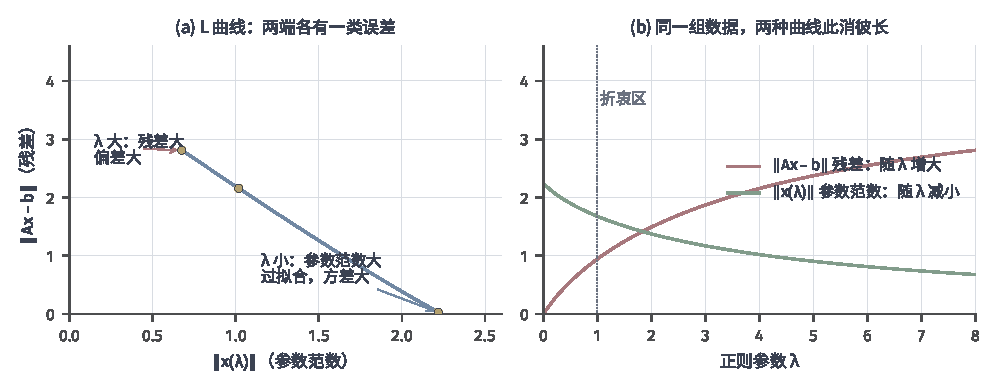
\includegraphics[width=168.998mm]{figures/01-mathematical-preliminaries-upper/02-linear-spaces/matplotlib/ls-regularization-bias-variance/ls-regularization-bias-variance.pdf}
  \caption{正则化的偏差—方差折中。$\bm A=\operatorname{diag}(2,1)$、$\bm b=(4,1)^\top$，
  岭解$\bm x(\lambda)=(8/(4+\lambda),1/(1+\lambda))^\top$。左：L曲线——横轴参数范数
  $\lVert\bm x(\lambda)\rVert$、纵轴残差$\lVert\bm A\bm x-\bm b\rVert$；右端（$\lambda$小）
  拟合准但参数大，左端（$\lambda$大）参数小但残差大。右：残差随$\lambda$上升、
  参数范数随$\lambda$下降，灰色虚线为折衷区。固定复算，无采样。}
  \label{fig:ls-regularization-bias-variance}
\end{figure*}

\section{二次优化}
\label{sec:ls-quadratic-optimization}

最小二乘目标本身是二次的；把“平方长度”推广到一般对称二次型，加上无约束、球面约束、
子空间约束与线性等式约束，得到一族可完全用代数配方和~\ref{sec:ls-svd}建立的谱定理
解决的优化问题。本节不使用微积分：所有最优性条件都由平方增量非负和正交关系得到。

\subsection{目标与约束}
\label{sec:ls-quadratic-goal}

一般二次目标写成（\term{二次型}，quadratic form）
\begin{equation}
 f(\bm x)=\frac12\bm x^\top\bm M\bm x+\bm c^\top\bm x,
 \label{eq:ls-general-quadratic}
\end{equation}
其中$\bm M$不必对称。反对称部分$\frac12(\bm M-\bm M^\top)$满足
$\bm x^\top(\bm M-\bm M^\top)\bm x=0$，故二次型只由对称部分
$\bm S=\frac12(\bm M+\bm M^\top)$决定，以下一律取$\bm S=\bm S^\top$。

无约束问题为$\min_{\bm x\in\mathbb R^d}f(\bm x)$；带线性等式约束为
\begin{equation}
 \min\ f(\bm x)\quad\text{s.t.}\quad \bm C\bm x=\bm d,
 \label{eq:ls-equality-constrained}
\end{equation}
$\bm C\in\mathbb R^{p\times d}$。可行性先于优化：$\bm C\bm x=\bm d$必须相容。

不含线性项时目标为$\bm x^\top\bm S\bm x$（可取$1/2$因子）。齐次性使目标在尺度缩放
下按平方变化，因而自然约束在单位球面$\lVert\bm x\rVert_2=1$、闭球
$\lVert\bm x\rVert_2\leq1$或某个子空间中；球面消除尺度自由度，只比较方向。

长度由$\bm B\succ0$度量时，约束为$\bm x^\top\bm B\bm x=1$，即\term{广义球面}；
它把加权长度固定，仍只优化方向。

\subsection{存在性与唯一性}
\label{sec:ls-quadratic-existence}

先判定目标在给定集合上是否有下界、极小点是否存在、是否唯一，再谈求解。

\subsubsection{无约束问题}
\label{sec:ls-unconstrained-existence}

先看三个二元例子区分目标形状：$f_1(x,y)=x^2+2y^2$恒正、原点是唯一谷底；
$f_2(x,y)=x^2$沿$y$轴整条等高，$f_2=0$取遍$(0,y)$，最小值集合是一条直线；
$f_3(x,y)=x^2-y^2$在原点一方向上谷、另一方向上脊，是鞍点。
图~\ref{fig:ls-quadratic-level-sets}把三类水平集并置：正定是同心椭圆，半正定退化为
平行直线槽，不定是双曲线。它们的差别只在$\bm S$的惯性（正、负、零特征值个数）。

\begin{figure*}[htbp]
  \centering
  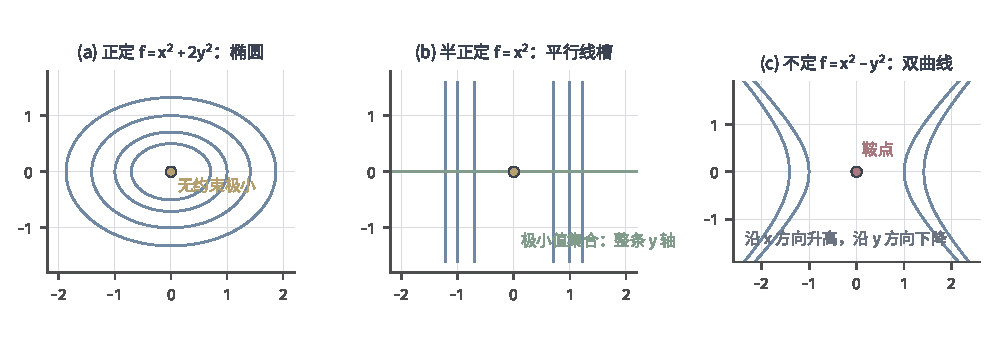
\includegraphics[width=168.998mm]{figures/01-mathematical-preliminaries-upper/02-linear-spaces/matplotlib/ls-quadratic-level-sets/ls-quadratic-level-sets.pdf}
  \caption{二次型水平集的三种情形。(a)正定$f=x^2+2y^2$：四层同心椭圆，黄点为唯一极小
  $(0,0)$；(b)半正定$f=x^2$：水平集退化为竖直线，绿线是极小值集合——整条$y$轴；
  (c)不定$f=x^2-y^2$：双曲线，红点为鞍点，沿$x$方向是谷、沿$y$方向是脊。
  解析式直接求值。}
  \label{fig:ls-quadratic-level-sets}
\end{figure*}

由谱引理~\ref{thm:ls-real-symmetric-spectral}，$\bm S$的正交谱展开把任意
$\bm x=\sum_i c_i\bm q_i$代入得
$f(\bm x)=\frac12\sum_i\lambda_i c_i^2+\sum_i c_i\bm c^\top\bm q_i$，每个方向独立。

若$\bm S$有负特征值$\lambda_j<0$，沿$\bm q_j$取$\bm x=t\bm q_j$，二次项
$\frac12\lambda_jt^2$按$t^2$趋向$-\infty$，线性项只按$t$一次增长，$|t|$足够大时
$t^2$项主导，目标无下界，不存在最小值。因此不定矩阵上的驻点不能当作最小点。

$\bm S\succeq0$时每个$\lambda_i\geq0$，二次项非负且沿正特征方向增长。零特征方向
$\lambda_j=0$上二次项为常数，目标只保留该方向的线性项；这些方向是否把目标拉向$-\infty$，
必须单独检查，不能因为二次项非负就认定有下界。

零方向$\bm q_j$上若有线性分量$\bm c^\top\bm q_j\neq0$，取$\bm x=t\bm q_j$，目标中的
线性项$t\,\bm c^\top\bm q_j$在$t\to-\infty$时趋向$-\infty$。故有下界的必要条件是
$\bm c\perp\ker\bm S$，由对称算子$\operatorname{range}\bm S=(\ker\bm S)^\perp$，
即$\bm c\in\operatorname{range}\bm S$。这也是正规方程$\bm S\bm x=-\bm c$相容的条件。

$\bm S\succ0$时所有$\lambda_i>0$，目标沿每个方向严格增长，唯一极小点。
$\bm S\succeq0$且$\bm c\in\operatorname{range}\bm S$时，正规方程相容，极小点存在
但沿$\ker\bm S$方向平坦，解集为仿射空间$\bm x_*+\ker\bm S$；不另加范数最小准则则
答案不唯一。

满足$\bm S\bm x+\bm c=0$的点只是驻点（最优性方程成立）。$\bm S$不定时，沿正特征方向
移动目标上升、沿负特征方向下降，驻点两侧一升一降，是鞍点而非最小点。不能把“方程成立”
当作“最小”，必须同时检查$\bm S$没有负方向；驻点条件只给出候选，不给出优劣判定。

\paragraph{惯性、合同判据与有界性}

$\bm S$的\term{惯性}（inertia）指正、负、零特征值的个数三元组$(n_+,n_-,n_0)$，由
谱引理唯一确定。目标有无下界恰由$n_-$判定：$n_->0$即存在负方向，目标无下界；
$n_-=0$（半正定）时二次项非负，目标有下界。合同变换（用可逆$\bm P$作
$\bm P^\top\bm S\bm P$）保持三个计数不变，故无需真的算出特征值，也可由对称消元记录
主元符号判断有界性。

\subsubsection{球面与子空间约束}
\label{sec:ls-sphere-existence}
\label{sec:linear-algebra-homogeneous-estimation}
\label{sec:linear-algebra-constrained-estimation}

单位球面$\{\bm x:\lVert\bm x\rVert_2=1\}$在有限维中是闭有界集，连续函数
$\bm x^\top\bm S\bm x$由~\ref{thm:ls-extreme-value}在球上同时取到最大值和最小值，
与$\bm S$是否正定无关；不定矩阵的两个极值分居零两侧。这一存在性不依赖方向是否可解，
先保证极值点存在，再讨论它落在哪个谱方向。

\paragraph{尺度消去与Rayleigh商}

齐次目标$\bm x^\top\bm S\bm x$在$\bm x\neq0$上按平方缩放变化，直接优化会被长度主导。
把长度约掉，方向评价写成\term{Rayleigh商}（Rayleigh quotient）
\begin{definition}[Rayleigh商]
\label{def:matrix-analysis-rayleigh-quotient}
\begin{equation}
 R_{\bm S}(\bm x)=\frac{\bm x^\top\bm S\bm x}{\bm x^\top\bm x},
 \label{eq:matrix-analysis-rayleigh-quotient}
\end{equation}
\end{definition}
它在$\bm x$缩放任意非零倍时不变，因此求$R_{\bm S}$的极值等价于在单位球面上求
$\bm x^\top\bm S\bm x$的极值，长度自由度被完全消去。

把$\bm x=\sum_i c_i\bm q_i$代入，分母$\sum_i c_i^2=1$（球面），
$R_{\bm S}(\bm x)=\sum_i\lambda_i c_i^2$是特征值以权重$c_i^2$（和为$1$）作的加权平均，
故落在$[\lambda_{\min},\lambda_{\max}]$内；令权重全给$\lambda_1$得最大值、全给
$\lambda_d$得最小值，且分别在$\bm q_1$、$\bm q_d$上取等。

$\lambda_i=\lambda_j$时，这两个特征向量的任意标准正交组合仍是该特征值的特征方向，
张成的子空间中每个单位向量都给出同一个极值商。故极值值唯一，达到它的方向一般不唯一；
仅当目标特征值单重时，方向才只差一个符号。图~\ref{fig:ls-sphere-constrained-extremum}
用一个二元对称矩阵把这一相切关系画出：极值椭圆恰在特征方向处与单位圆相切。

\begin{figure}[htbp]
  \centering
  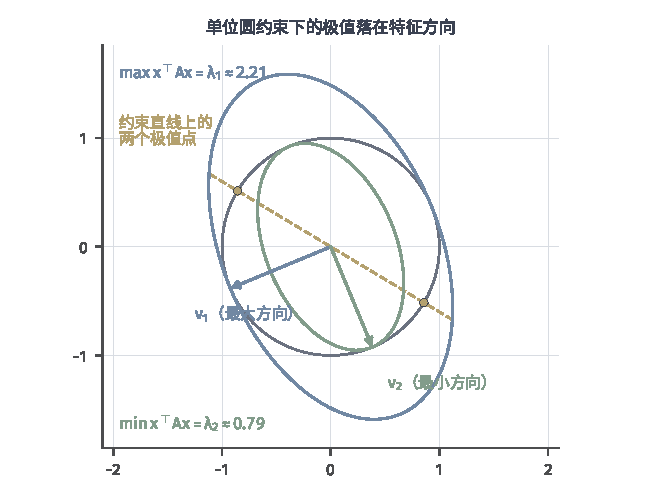
\includegraphics[width=112mm]{figures/01-mathematical-preliminaries-upper/02-linear-spaces/matplotlib/ls-sphere-constrained-extremum/ls-sphere-constrained-extremum.pdf}
  \caption{单位圆约束下的极值落在特征方向。$\bm S=\left[\begin{smallmatrix}2&0.5\\0.5&1\end{smallmatrix}\right]$，
  灰圆为$\lVert\bm x\rVert=1$。蓝椭圆$\bm x^\top\bm S\bm x=\lambda_1\approx2.21$在
  $\pm\bm v_1$处与单位圆相切（最大值），绿椭圆$=\lambda_2\approx0.79$在$\pm\bm v_2$处
  相切（最小值）；黄色虚线为子空间约束直线，其上黄点是该约束下的两个极值。
  $\lambda_{1,2}=(3\pm\sqrt2)/2$。固定复算。}
  \label{fig:ls-sphere-constrained-extremum}
\end{figure}

闭球$\lVert\bm x\rVert\leq1$是有界闭集，极值同样存在。$\bm S\succeq0$时最小值$0$
在内部$\bm x=0$取到，方向问题因此被迫放到边界；$\bm S$不定时最小值为负，落在
边界球面上，内部只含$\bm x=0$这个平凡点。所以“非零方向估计”必须主动固定单位长度，
否则齐次目标会把平凡解$\bm x=0$当作答案。

\paragraph{子空间约束下的同一问题}

限制在子空间$\mathcal W$中，问题仍是$\min_{\bm x\in\mathcal W}R_{\bm S}(\bm x)$，
由$\mathcal W$上的限制谱决定，是特征值交错与广义特征问题的入口。典型应用是
\term{齐次最小二乘}（homogeneous least squares）：模型写成$\bm A\bm h\approx\bm0$，
直接最小化$\lVert\bm A\bm h\rVert_2^2$总会接受平凡解$\bm h=\bm0$，必须先固定非零尺度：
\begin{equation}
 \min_{\lVert\bm h\rVert_2=1}\ \lVert\bm A\bm h\rVert_2^2
 =\min_{\lVert\bm h\rVert_2=1}\bm h^\top\bm A^\top\bm A\bm h.
 \label{eq:linear-algebra-homogeneous-least-squares}
\end{equation}
由Rayleigh--Ritz，最小值为$\bm A^\top\bm A$的最小特征值，最优$\bm h$是对应单位特征向量，
即最弱右奇异方向。$\bm A$有非零零空间时最小值为零，任一单位零空间向量都达到最优；
特别地$m<d$时不能只看紧致SVD列出的正奇异值而漏掉右零空间。最小特征值单重时方向只差
符号，重数更大则比例也不足以唯一确定。例如$\bm A=[\,1\ -2\,]$只要求$h_1=2h_2$，
单位解为$\pm(2,1)^\top/\sqrt5$，两个符号表示同一个实比例。

\subsubsection{线性等式约束}
\label{sec:ls-equality-existence}

优化只在可行集上进行，先判定$\bm C\bm x=\bm d$相容（$\bm d\in\operatorname{range}\bm C$）；
不相容时没有可行点，问题无解，谈不上优化。相容但$\bm C$的行线性相关时，多余方程是
独立方程的线性组合，不改变可行集，求解前可先去冗余，缩小约束规模。

取一个特解$\bm x_0$满足$\bm C\bm x_0=\bm d$，令$\mathcal N=\ker\bm C$，其标准正交基
排成矩阵$\bm N$。于是$\bm C(\bm x-\bm x_0)=\bm0$当且仅当$\bm x-\bm x_0\in\mathcal N$，
全部可行点参数化为$\bm x=\bm x_0+\bm N\bm z$，$\bm z$自由；可行方向就是$\mathcal N$。

把参数化代入$f(\bm x)=\frac12\bm x^\top\bm S\bm x+\bm c^\top\bm x$，二次项化为
$\bm z^\top(\bm N^\top\bm S\bm N)\bm z$，一次项化为
$\bm z^\top\bm N^\top(\bm c+\bm S\bm x_0)$，常数项与$\bm z$无关；问题化为
$\bm N^\top\bm S\bm N$在$\bm z$上的无约束二次问题，只在可行方向内检查曲率。

$\bm N^\top\bm S\bm N$在$\mathcal N$上正定，即$\bm z\neq0$时
$\bm z^\top\bm N^\top\bm S\bm N\bm z>0$；此时约化目标严格凸，唯一可行极小点，
代回参数化即得唯一$\hat{\bm x}$。

$\bm N^\top\bm S\bm N\succeq0$时，约化线性项$\bm N^\top(\bm c+\bm S\bm x_0)$
必须落在其值域内；若它沿某个零方向有分量，沿该方向移动时二次项不变而线性项下降，
目标无下界。条件满足时解集为$\bm x_*+\ker(\bm N^\top\bm S\bm N)$的仿射空间。

约化二次型在$\mathcal N$上有负方向，则沿该方向取$\bm x=\bm x_0+t\bm N\bm z$，
二次项按$t^2$趋向$-\infty$，约束问题无下界，与无约束情形同理。

\subsection{直接求解}
\label{sec:ls-quadratic-direct}

\subsubsection{无约束二次最小化}
\label{sec:ls-unconstrained-solve}

$\bm S\succ0$时把二次项配成完全平方：取$\bm x_*$满足$\bm S\bm x_*=-\bm c$，则
\[
 f(\bm x)-f(\bm x_*)=\frac12(\bm x-\bm x_*)^\top\bm S(\bm x-\bm x_*),
\]
右端因$\bm S$正定而非负，且只在$\bm x=\bm x_*$时为零。故$\bm S\bm x_*=-\bm c$给出
唯一最优线性方程，最小化问题归结为解这个正定对称方程。

$\bm S$正定，复用~\ref{sec:ls-direct-methods}的Cholesky分解$\bm S=\bm L\bm L^\top$，
先前代解$\bm L\bm y=-\bm c$，再回代解$\bm L^\top\bm x_*=\bm y$，避免形成逆矩阵。
分解与右端多重时可共享；这一路线与最小二乘正规方程用的是同一条正定对称求解流程。

$\bm S\succeq0$且$\bm c\in\operatorname{range}\bm S$时，$\bm S\bm x_*=-\bm c$相容。
由配方，任一解$\bm x_*$都是极小点；沿$\ker\bm S$移动二次项不变，全部解为
$\bm x_*+\ker\bm S$的仿射空间。不另加范数最小准则则答案不唯一，选代表的方法与普通
最小二乘的零空间选择相同。

核验两点：最优性方程$\bm S\hat{\bm x}+\bm c=0$成立；且对任意$\bm x$，增量
$\frac12(\bm x-\hat{\bm x})^\top\bm S(\bm x-\hat{\bm x})\geq0$非负。若增量沿某方向
为负，则该点不是最小点；方程成立只说明候选，符号检查才给出最小性。

\subsubsection{球面与子空间极值}
\label{sec:ls-sphere-solve}

\begin{theorem}[Rayleigh--Ritz]
\label{thm:matrix-analysis-rayleigh-ritz}
\label{eq:matrix-analysis-rayleigh-ritz}
设$\bm S$谱分解$\bm S=\sum_i\lambda_i\bm q_i\bm q_i^\top$，
$\lambda_1\geq\cdots\geq\lambda_d$，则
\begin{equation}
 \max_{\bm x\neq0}R_{\bm S}(\bm x)=\lambda_1\ \text{（在}\bm q_1\text{取到）},\qquad
 \min_{\bm x\neq0}R_{\bm S}(\bm x)=\lambda_d\ \text{（在}\bm q_d\text{取到）}.
\end{equation}
\end{theorem}
\begin{proof}
由谱展开$R_{\bm S}(\bm x)$是特征值的加权平均，故介于$\lambda_d$与$\lambda_1$之间；
取$\bm x=\bm q_1$、$\bm x=\bm q_d$时分别等于$\lambda_1$、$\lambda_d$，夹逼得端点取等。
\end{proof}

单方向极值只给$\lambda_1$与$\lambda_d$。要刻画中间的$\lambda_k$，取任意$k$维子空间
$\mathcal V$：它与$\operatorname{span}\{\bm q_k,\dots,\bm q_d\}$（维数$d-k+1$）的
维数之和$k+(d-k+1)=d+1>d$，故必有非零交点，交点处的Rayleigh商不大于$\lambda_k$。
换一个$d-k+1$维子空间与$\operatorname{span}\{\bm q_1,\dots,\bm q_k\}$同理相交。
这一维数交点关系是Courant--Fischer最小最大原理的几何来源。

\paragraph{Courant--Fischer的上下界与取等}

\begin{theorem}[Courant--Fischer]
\label{thm:matrix-analysis-courant-fischer}
\label{eq:matrix-analysis-courant-fischer}
\begin{equation}
 \lambda_k=\max_{\dim\mathcal V=k}\ \min_{\bm x\in\mathcal V,\bm x\neq0}R_{\bm S}(\bm x)
 =\min_{\dim\mathcal W=d-k+1}\ \max_{\bm x\in\mathcal W,\bm x\neq0}R_{\bm S}(\bm x).
\end{equation}
\end{theorem}
\begin{proof}
取$\mathcal V=\operatorname{span}\{\bm q_1,\dots,\bm q_k\}$，其中任意单位向量的
Rayleigh商不小于$\lambda_k$，给出下界；任一$k$维子空间与$\operatorname{span}\{\bm q_k,\dots,\bm q_d\}$
相交，交点处商不大于$\lambda_k$，给出上界。另一式由正交补同理得到。
\end{proof}
它不要求预先知道特征向量，为只需要第$k$个极值的子空间搜索提供了存在性表述。

\paragraph{正交列约束下的迹极值}

给定$k$个标准正交列$\bm V\in\mathbb R^{d\times k}$（$\bm V^\top\bm V=\bm I_k$），
\begin{theorem}[迹极值]
\label{thm:matrix-analysis-trace-minimum}
\label{eq:matrix-analysis-trace-minimum}
\begin{equation}
 \min_{\bm V^\top\bm V=\bm I_k}\operatorname{tr}(\bm V^\top\bm S\bm V)
 =\sum_{i=d-k+1}^d\lambda_i,
 \qquad
 \max_{\bm V^\top\bm V=\bm I_k}\operatorname{tr}(\bm V^\top\bm S\bm V)
 =\sum_{i=1}^k\lambda_i,
\end{equation}
\end{theorem}
\begin{proof}
由谱展开$\operatorname{tr}(\bm V^\top\bm S\bm V)=\sum_i\lambda_i\lVert\bm q_i^\top\bm V\rVert_2^2$，
权重$\lVert\bm q_i^\top\bm V\rVert_2^2$非负且总和为$k$；把权重配给最小的$k$个
$\lambda_i$得最小值，配给最大的$k$个得最大值，对应特征向量张成达到取等。
\end{proof}
最小值由$k$个最小特征向量张成，最大值由$k$个最大特征向量张成；这是后续正交拟合与
低秩方向提取的代数基础。

广义约束$\bm x^\top\bm B\bm x=1$、$\bm B\succ0$，先由Cholesky
$\bm B=\bm R^\top\bm R$令$\bm z=\bm R\bm x$，则约束化为$\lVert\bm z\rVert_2=1$，
目标$\bm x^\top\bm S\bm x$化为$\bm z^\top\bm R^{-\top}\bm S\bm R^{-1}\bm z$，成为
普通对称矩阵$\bm R^{-\top}\bm S\bm R^{-1}$的Rayleigh商，可直接用单方向极值结论。

\paragraph{广义特征问题与方向恢复}

\begin{definition}[广义特征值]
\label{def:matrix-analysis-generalized-eigenvalue}
白化后的对称问题等价于\term{广义特征问题}
\begin{equation}
 \bm S\bm v=\mu\bm B\bm v,
 \label{eq:matrix-analysis-generalized-eigenproblem}
\end{equation}
\end{definition}
白化后普通特征向量$\bm z$恢复原方向$\bm v=\bm R^{-1}\bm z$；广义极值即$\mu$的最大、
最小值，方向按此恢复。不要直接对$\bm B^{-1}\bm S$（一般非对称）求特征，其特征值可能为
复数而失去极值意义。

\subsubsection{等式约束二次最小化}
\label{sec:ls-equality-solve}

由可行点参数化$\bm x=\bm x_0+\bm N\bm z$，把约束消去后，目标化为$\bm z$上的无约束
二次问题，正规方程为
$(\bm N^\top\bm S\bm N)\bm z=-\bm N^\top(\bm c+\bm S\bm x_0)$；解出$\bm z$后按
$\bm x=\bm x_0+\bm N\bm z$拼回原变量。这一路线先把可行性编入参数化，求解时不必再
显式处理约束。

约化矩阵$\bm N^\top\bm S\bm N$正定即按无约束流程Cholesky求解，得到唯一$\hat{\bm z}$；
半正定则按值域条件解相容方程，在全部最小点中选代表。约化矩阵维数等于$\ker\bm C$的
维数，通常小于原问题规模。

对任意可行方向$\bm\delta$（$\bm C\bm\delta=0$），目标沿$\bm\delta$的一阶变化为
$\bm\delta^\top(\bm S\bm x+\bm c)$，最优性要求它为零。这说明$\bm S\bm x+\bm c$正交于
$\ker\bm C$，由正交补关系落在$\operatorname{range}(\bm C^\top)$，故存在乘子$\bm\mu$
使$\bm S\bm x+\bm c=\bm C^\top\bm\mu$；$\bm\mu$衡量约束方向上的平衡量。

\paragraph{KKT系统的分块构造}

联立约束$\bm C\bm x=\bm d$与最优性$\bm S\bm x+\bm c=\bm C^\top\bm\mu$，得到
\term{KKT条件}（KKT conditions）分块系统
\begin{equation}
 \begin{bmatrix}\bm S&\bm C^\top\\ \bm C&\bm0\end{bmatrix}
 \begin{bmatrix}\bm x\\ \bm\mu\end{bmatrix}
 =\begin{bmatrix}-\bm c\\ \bm d\end{bmatrix}.
 \label{eq:ls-kkt-system}
\end{equation}
它同时编码可行性（第二块行）与最优性（第一块行），由正交关系推出，不需要微分记号。

对分块系统可先消元（把$\bm\mu$从第一行解出代回），或对分块矩阵作适当分解直接求解，
同时得到$\bm x$与$\bm\mu$。$\bm\mu$只是伴随约束的对偶量，不改变原目标值，核验时
主要保证$\bm x$满足原目标与约束。

$\ker\bm C\cap\ker\bm S=\{\bm0\}$时$\bm\mu$唯一；约束冗余（$\bm C$行相关）时
$\operatorname{range}\bm C^\top$维数小于行数，$\bm\mu$可加$\ker\bm C^\top$中的量而
不改变方程，乘子不唯一，但可行方向正定时原变量$\bm x$仍可唯一。

分别核验：可行性$\bm C\hat{\bm x}=\bm d$；最优性$\bm S\hat{\bm x}+\bm c\in\operatorname{range}(\bm C^\top)$，
即对所有$\bm\delta\in\ker\bm C$有$\bm\delta^\top(\bm S\hat{\bm x}+\bm c)=0$。只满足约束
或只满足方程都不是合格最小点，二者缺一不可。

\subsection{迭代求解}
\label{sec:ls-quadratic-iterative}

直接法需要分解矩阵；只给矩阵作用时用迭代逼近谱方向或正定极小点，收敛速度证明留待
迭代收敛章节。

$\bm S\succ0$的无约束问题$\bm S\bm x=-\bm c$本身就是正定对称线性方程，直接复用
~\ref{sec:ls-krylov-methods}的共轭梯度法：每步只调用$\bm S$对向量的乘积，不形成分解，
更新格式、有限步终止与停止核验在该处建立，此处不重述。

求最大特征方向时反复$\bm v\leftarrow\bm S\bm v/\lVert\bm S\bm v\rVert_2$：每次作用把
最大特征值方向按$\lambda_1$放大，其余方向按比值$\lambda_i/\lambda_1$相对缩小，归一化
后方向逐次偏向$\bm q_1$。相邻特征值分离越快，比值越小，方向提取越直接；分离程度决定
收敛快慢，定量速率留待迭代收敛章节。

求靠近$\rho$的特征方向时迭代$(\bm S-\rho\bm I)^{-1}\bm v$，要求$\bm S-\rho\bm I$可逆
（$\rho$不是特征值）。移位后靠近$\rho$的特征值变为大数，其分量被逐步放大；每步解一个
移位线性系统而非求逆矩阵，收敛速度由目标与邻近特征值的距离决定。

Lanczos用短递推把$\bm S$投影成三对角小矩阵，在小矩阵上求极值方向再经基映回原空间；
只调用乘积、存储随步数线性增长，适合只需要少数几个极值方向、矩阵不能整体分解的情形。
有限步理论与收敛速率属迭代收敛章节。

\section{矩阵低秩逼近}
\label{sec:ls-matrix-low-rank}
\label{sec:matrix-analysis-svd-low-rank}
\label{sec:ch06-rank-constrained-approximation}
\label{sec:ch06-error-constrained-rank}

第~\ref{sec:ls-least-squares}节在固定形状的输入向量中挑选系数，使输出残差最小；
本节改变任务对象：未知量本身是一张矩阵，要求它在保持主要作用的同时占用更少参数。
一张$m\times n$稠密矩阵需要存储$mn$个数，每次作用需要$O(mn)$次运算；推荐系统的评分
矩阵、一幅图像或一批样本的设计矩阵，$mn$轻易达到百万级，直接存储和运算都不现实。
这类矩阵的信息常高度集中：少数几个输入方向被放大后送入配对的输出方向，就解释了大部分
作用。自然的问题是：能否只保留最重要的$k$个方向，用远少于$mn$的参数近似整张矩阵？
若能以$k$个输入输出方向的配对近似它，存储和作用成本便可降到$O((m+n)k)$。

特征向量要求输出回到输入的同一方向，因而适合分析同一空间内的反复作用；压缩却要问哪些
输入方向的作用最值得保留，并允许输出落到另一个方向。三维输入送入二维输出时已经无法要求
两端沿同一条方向；又如把用户作为行、影片作为列，评分矩阵$\bm R\in\mathbb R^{n_{\mathrm u}\times n_{\mathrm m}}$
中$\bm v\mapsto\bm R\bm v$把影片坐标映到用户坐标，两端本就是不同对象的坐标，谈不上同一个
特征方向。因此本节使用第~\ref{sec:ls-svd}节已经建立的奇异值分解：定义域与陪域各自选取
正交方向，有非零作用的输入方向分别被缩放后送入配对的输出方向，其余方向映为零。
存在性与构造不再重复，本节只在这一工具上回答规模怎样度量、最优候选是谁、怎样计算与核验。

\subsection{目标与误差}
\label{sec:ls-low-rank-objective}

\paragraph{秩预算与误差范数}

先规定规模预算：给定整数$k$，在所有秩不超过$k$的矩阵中寻找离$\bm A$最近的候选
$\bm B$。误差口径先于方向选择确定，常用两种：谱范数误差
$\lVert\bm A-\bm B\rVert_2=\max_{\lVert\bm x\rVert_2=1}\lVert(\bm A-\bm B)\bm x\rVert_2$
度量任意单位输入的最坏输出偏差；Frobenius误差
$\lVert\bm A-\bm B\rVert_{\mathrm F}=(\sum_{i,j}(a_{i,j}-b_{i,j})^2)^{1/2}$
对一组标准输入方向的输出偏差平方求和后开方。两者回答不同问题：前者保证最坏方向不失真，
后者累计全部坐标的总偏差，不能互相替代。

由~\ref{thm:ls-svd-existence}，$\bm A\in\mathbb R^{m\times n}$有分解
$\bm A=\bm U\bm\Sigma\bm V^\top$，非零奇异值按降序记为
$\sigma_1\geq\cdots\geq\sigma_r>0$，$r=\operatorname{rank}\bm A$。
下面所有结论都以这一给定分解为输入，不再重新证明奇异值的存在性。

\paragraph{秩约束与核范数惩罚的区别}

固定秩约束$\operatorname{rank}\bm B\leq k$是一个硬预算：可行集合由若干低维线性流形
拼成，不是凸集，候选不能沿线段自由插值。另一条路线不在参数上设限，而在拟合目标中附加
对矩阵“大小”的凸惩罚：
\begin{equation}
 \min_{\bm B}\ \tfrac12\lVert\bm A-\bm B\rVert_{\mathrm F}^2
 +\lambda\lVert\bm B\rVert_*,
 \qquad \lambda\geq0,
 \label{eq:ls-nuclear-penalty-problem}
\end{equation}
其中$\lVert\cdot\rVert_*$是稍后定义的核范数。惩罚改变的是目标本身：$\lambda$越大，
保留下来的奇异尺度被压得越小，它产生的实际秩取决于原谱，不等于直接指定$k$。
硬预算回答“最多用$k$个方向能做到多好”，惩罚问题回答“拟合与简洁之间怎样折中”，
两者的最优解一般不同，求解路径也不同，不能不加说明地当成同一个截断问题。

\subsection{规模与误差的比较}
\label{sec:ls-rank-scale-comparison}

\subsubsection{秩与保留信息}
\label{sec:ls-rank-and-information}

\paragraph{精确非零方向与代数秩}

代数秩$r=\operatorname{rank}\bm A$是非零奇异值的个数，也就是$\bm A$真正使用的
精确非零方向数：$\bm A=\sum_{i=1}^r\sigma_i\bm u_i\bm v_i^\top$中每一项对应一对
独立的伸缩方向，$\sigma_i=0$的方向不参与作用。代数秩是离散整数，对任意小的秩增加
扰动都可能跳变：$\operatorname{diag}(1,\varepsilon)$的代数秩恒为$2$，尽管
$\varepsilon\to0$时第二个方向的作用趋于消失。因此它描述“精确表示需要几项”，
不直接回答“近似表示保留几项足够”。

\paragraph{容差与数值秩}

数据带有噪声时，把低于某一绝对阈值$\tau$的奇异值视为零更符合实际。\term{数值秩}
（numerical rank）定义为
\begin{equation}
 r_{\mathrm{num}}(\bm A;\tau)=\#\{i:\sigma_i>\tau\}.
 \label{eq:ls-numerical-rank}
\end{equation}
它恰好等于谱范数误差不超过$\tau$时所需的最小秩（见~\ref{sec:ls-low-rank-solve}），
但必须同时说明阈值口径：绝对阈值$\tau$与相对阈值$\tau=\epsilon\lVert\bm A\rVert_2$
给出不同计数，零矩阵不能计算$0/0$。数值秩不是一个不含容差的固定数值，换一个阈值
就换一个数。

\paragraph{谱能量分布与稳定秩}

代数秩和数值秩都是整数计数，能量集中程度则需要一个连续尺度。非零矩阵$\bm A$的
\term{稳定秩}（stable rank）\label{def:matrix-analysis-stable-rank}定义为
\begin{equation}
 r_{\mathrm{stable}}(\bm A)
 =\frac{\lVert\bm A\rVert_{\mathrm F}^2}{\lVert\bm A\rVert_2^2}
 =\frac{\sum_{i=1}^r\sigma_i^2}{\sigma_1^2},
 \label{eq:matrix-analysis-stable-rank}
\end{equation}
零矩阵另约定为零。由$\sigma_1^2\leq\sum_i\sigma_i^2\leq r\sigma_1^2$，
$1\leq r_{\mathrm{stable}}\leq r$：所有非零奇异值相等时取到$r$，能量几乎全在
首方向时接近$1$。例如奇异值$(8,3,1,0.2)$的稳定秩为
$74.04/64\approx1.157$，说明能量高度集中在第一个方向，尽管代数秩是$4$。

\paragraph{有效秩的不同归一化口径}

稳定秩是\term{有效秩}（effective rank）的一种，另一种常用口径把奇异值归一化为
概率分布$p_i=\sigma_i/\sum_j\sigma_j$，再取熵的指数
\begin{equation}
 r_{\mathrm{ent}}(\bm A)
 =\exp\!\left(-\sum_i p_i\log p_i\right),
 \qquad 0\log0=0.
 \label{eq:ls-effective-rank-entropy}
\end{equation}
也有版本用平方奇异值归一化$p_i=\sigma_i^2/\sum_j\sigma_j^2$，两种口径数值一般不同。
它们都是连续的能量分散度，不是误差阈值下的最优整数秩：上例的$1.157$既不是
$\tau=1$时的谱最优秩$2$，也不是Frobenius最优秩$3$。它也不同于后续正则化讨论中
随惩罚尺度变化的核有效维度，不要混用。

\paragraph{零矩阵与连续性边界}

稳定秩在非零矩阵处连续且不随整体缩放改变（分子分母同乘$c^2$），但零矩阵的约定值$0$
不使它在零处连续：$\operatorname{diag}(1,\varepsilon)$的稳定秩趋于$1$而不是$0$。
有效秩的各归一化口径有同样的边界行为。因此涉及零矩阵时必须单独处理，不能把连续尺度
公式直接代入；工程上先判$\bm A=\bm0$再计算任何比值。

\paragraph{规模指标与最小可行秩的区别}

代数秩、数值秩、稳定秩与有效秩回答不同问题：代数秩是精确表示的项数，数值秩是阈值下的
计数，稳定秩和有效秩是能量分散的连续描述；而“给定误差预算至少要保留几项”是
~\ref{sec:ls-low-rank-solve}要解的优化问题的答案。规模指标不能代替误差预算，
误差预算也不给出能量分散度。此外，谱范数次乘
$\lVert\bm A_L\cdots\bm A_1\rVert_2\leq\prod_\ell\lVert\bm A_\ell\rVert_2$
不蕴含稳定秩可以逐层相乘：各层的最强方向未必对齐，上界可能宽松。

\subsubsection{误差与方向选择}
\label{sec:ls-direction-pairing}

\paragraph{固定奇异值下的方向选择}

求最佳低秩候选之前，先解决一个更一般的子问题：固定候选$\bm B$的奇异值$s_1\geq\cdots\geq0$，
只让它的左右奇异方向自由，怎样配对才能使$\bm B$离$\bm A$最近？这一子问题同时服务于
固定秩截断和核范数惩罚，结论被~\ref{sec:ls-orthogonal-approximation}节与
~\ref{sec:ls-symmetric-spectral-approximation}节复用。

\paragraph{迹展开与方向配对权重}

设$\bm A=\bm U\Sigma\bm V^\top$，$\bm B=\widehat{\bm U}\widehat\Sigma\widehat{\bm V}^{\,\top}$，
两端标准内积为Frobenius配对$\langle\bm X,\bm Y\rangle_{\mathrm F}
=\operatorname{tr}(\bm X^\top\bm Y)$（见~\ref{sec:ls-matrix-contractions}）。
展开平方距离的交叉项：
\begin{equation}
 \operatorname{tr}(\bm B^\top\bm A)
 =\sum_{i,j}s_i\sigma_j
   (\widehat{\bm u}_i^\top\bm u_j)(\widehat{\bm v}_i^\top\bm v_j).
 \label{eq:ls-trace-pairing-expand}
\end{equation}
令$c_{i,j}=|\widehat{\bm u}_i^\top\bm u_j|\,|\widehat{\bm v}_i^\top\bm v_j|$，
距离中的交叉项只通过这个配对权重依赖方向。

\paragraph{配对权重的行列和约束}

固定$i$，由Cauchy--Schwarz与正交投影不增加长度，
$\sum_j|\widehat{\bm u}_i^\top\bm u_j|^2\leq1$、
$\sum_j|\widehat{\bm v}_i^\top\bm v_j|^2\leq1$，故
\begin{equation}
 \sum_j c_{i,j}\leq1,\qquad
 \sum_i c_{i,j}\leq1.
 \label{eq:ls-pairing-weight-marginals}
\end{equation}
每行、每列的权重和都不超过$1$，总权重和不超过$\min(m,n)$。

\paragraph{有序奇异值的配对上界与取等}

把奇异值写成相邻差分的和，前$k$行、前$\ell$列的权重和$C_{k,\ell}\leq\min(k,\ell)$，
于是
\begin{equation}
 \sum_{i,j}\alpha_i\beta_j c_{i,j}
 \leq\sum_{i=1}^q\alpha_i\beta_i,
 \qquad
 \alpha_i=\sigma_i(\bm A),\ \beta_i=s_i(\bm B)
 \text{ 均降序排列}.
 \label{eq:ls-rearrangement-trace-bound}
\end{equation}
差分展开后$\min(k,\ell)=\sum_i\mathbf 1\{i\leq k,\ i\leq\ell\}$，两侧分别求差分和即得。
上界在$\bm B$与$\bm A$使用相同左右奇异方向时取等：$\widehat{\bm u}_i=\bm u_i$、
$\widehat{\bm v}_i=\bm v_i$。这就是有序奇异值的配对不等式：大配大、小配小不损失配对，
交叉配对只会减小$\operatorname{tr}(\bm B^\top\bm A)$。

\paragraph{Schatten范数的对偶表达}

由配对上界可以建立一族矩阵尺度。对$1\leq p<\infty$，\term{Schatten $p$范数}
（Schatten $p$-norm）定义为
\begin{equation}
 \lVert\bm A\rVert_{S_p}
 =\left(\sum_i\sigma_i^p\right)^{1/p},
 \qquad
 \lVert\bm A\rVert_{S_\infty}=\sigma_1,
 \label{def:matrix-analysis-schatten-norm}
\end{equation}
零矩阵的值为零。$p=1,2,\infty$依次给出核范数
$\lVert\bm A\rVert_*=\sum_i\sigma_i$\label{eq:matrix-analysis-nuclear-norm}、Frobenius范数
$\lVert\bm A\rVert_{\mathrm F}=(\sum_i\sigma_i^2)^{1/2}$\label{eq:matrix-analysis-frobenius-norm}与谱范数
$\lVert\bm A\rVert_2=\sigma_1$\label{eq:matrix-analysis-spectral-norm}；这三个谱表达式是~\ref{thm:ls-svd-existence}的直接推论，
不再重复推导。Schatten范数在两端正交换基下不变，只关心伸缩谱。

标量Hölder不等式给出对偶关系：对共轭指数$1/p+1/q=1$，
\begin{equation}
 \lVert\bm A\rVert_{S_p}
 =\max_{\lVert\bm B\rVert_{S_q}\leq1}
 |\operatorname{tr}(\bm B^\top\bm A)|.
 \label{eq:ls-schatten-duality}
\end{equation}
取达到构造：$1<p<\infty$时令$\bm B$与$\bm A$同方向、奇异值
$b_i=\sigma_i^{p-1}/\lVert\bm A\rVert_{S_p}^{p-1}$；$p=1$时在每个正奇异方向取
$b_i=1$；$p=\infty$时只在最大奇异方向取$b_i=1$。$\bm A=\bm0$时取$\bm B=\bm0$。
因此核范数是谱范数的对偶，Frobenius范数自对偶。

\paragraph{三角不等式与核范数合法性}

线性配对在单位球上的最大值自动满足三角不等式、齐次性与正定性，所以对偶是范数；
核范数作为谱范数的对偶，本身是合法范数，其单位球凸，~\eqref{eq:ls-nuclear-penalty-problem}
是凸优化问题。$0<p<1$沿用同一公式只得到拟范数：
$\bm A=\operatorname{diag}(1,0)$、$\bm B=\operatorname{diag}(0,1)$时
$\lVert\bm A+\bm B\rVert_{S_p}=2^{1/p}>2$，违反三角不等式，不能当作凸惩罚使用。

\paragraph{秩相关的范数比较}

对秩为$r$的矩阵，由$\sigma_1\leq(\sum_i\sigma_i^p)^{1/p}$等逐项比较得到
\begin{equation}
 \lVert\bm A\rVert_2\leq\lVert\bm A\rVert_{\mathrm F}
 \leq\sqrt r\,\lVert\bm A\rVert_2,\qquad
 \lVert\bm A\rVert_{\mathrm F}\leq\lVert\bm A\rVert_*
 \leq\sqrt r\,\lVert\bm A\rVert_{\mathrm F}.
 \label{eq:matrix-analysis-norm-rank-relations}
\end{equation}
常数带秩因子，范数等价在这里不是无代价的。多个方向同时被舍弃时，最坏方向误差
（谱口径）和总平方误差（Frobenius口径）不能用同一个舍弃奇异值代替。
\subsection{存在性与唯一性}
\label{sec:ls-low-rank-existence}

\paragraph{最佳低秩近似的存在性}

固定$k$，可行集合$\{\bm B:\operatorname{rank}\bm B\leq k\}$是所有$(k+1)$阶子式
同时为零的集合，因而是闭集。取使$\lVert\bm A-\bm B\rVert$收敛到下确界的极小化序列
$\bm B_t$，它必有界：否则由三角不等式
$\lVert\bm B_t\rVert\leq\lVert\bm A\rVert+\lVert\bm A-\bm B_t\rVert$，而误差序列
有界。有限维中闭有界集上的连续范数函数取到极值（~\ref{thm:ls-extreme-value}），
故极限$\bm B_*$仍在可行集合内并达到最小误差。谱范数与Frobenius范数下存在性相同，
区别只在最优解是否唯一。

\paragraph{奇异值间隙与Frobenius最优解的唯一性}

Frobenius目标下，当$1\leq k<r$且$\sigma_k>\sigma_{k+1}$有严格间隙时，最佳矩阵唯一：
严格间隙迫使最优保留子空间恰好由前$k$个右奇异向量张成，误差平方的对齐项又把投影结果
确定下来。边界奇异值相等时，对应重特征子空间内的任意标准正交旋转仍给出同一最优值，
最佳矩阵不唯一，但最佳值唯一。

\paragraph{谱范数误差下的非唯一性}

谱目标即使有严格间隙也未必唯一。例如$\bm A=\operatorname{diag}(2,0.4)$，
$\bm B_t=\operatorname{diag}(2+t,0)$对$|t|\leq0.4$都以谱误差$0.4$近似$\bm A$，
候选矩阵互不相同。因此谱口径下只能保证最佳值$\sigma_{k+1}$达到，不能宣称唯一候选；
需要唯一解时应改用Frobenius口径并检查间隙。

\subsection{秩约束的求解}
\label{sec:ls-low-rank-solve}

\subsubsection{基于完整分解的求解}
\label{sec:ls-full-svd-solve}

\paragraph{截断SVD候选的构造}

取前$k$个奇异方向构造候选\term{截断SVD}（truncated SVD）
\begin{equation}
 \bm A_k=\sum_{i=1}^k\sigma_i\bm u_i\bm v_i^\top,
 \qquad 0\leq k<r,
 \label{eq:matrix-analysis-truncated-svd}
\end{equation}
$k=0$为空和$\bm0$。它只保留最大的$k$个伸缩方向，尾部$\bm A-\bm A_k$由剩余奇异项
组成。

\paragraph{谱误差与Frobenius误差}

由分解形式直接读出两种误差：
\begin{equation}
 \lVert\bm A-\bm A_k\rVert_2=\sigma_{k+1},\qquad
 \lVert\bm A-\bm A_k\rVert_{\mathrm F}
 =\left(\sum_{i=k+1}^r\sigma_i^2\right)^{1/2}.
 \label{eq:ls-truncated-errors}
\end{equation}
谱误差是尾部最大奇异值，Frobenius误差是尾部能量开方；只舍弃一个方向时两者相等，
多个尾方向时必须分别取最大值与平方和。

\paragraph{任意低秩候选的误差下界}

截断候选为什么最优，需要对任意秩不超过$k$的$\bm B$证明误差不能更小。谱口径：
$S=\operatorname{span}\{\bm v_1,\ldots,\bm v_{k+1}\}$为$k+1$维，而
$\dim\ker\bm B\geq n-k$，二者必有非零交向量。取单位向量
$\bm x=\sum_{i=1}^{k+1}c_i\bm v_i\in S\cap\ker\bm B$，则
\begin{equation}
 \lVert(\bm A-\bm B)\bm x\rVert_2
 =\lVert\bm A\bm x\rVert_2
 =\left(\sum_{i=1}^{k+1}\sigma_i^2c_i^2\right)^{1/2}
 \geq\sigma_{k+1}.
 \label{eq:ls-spectral-lower-bound}
\end{equation}
Frobenius口径：令$\bm C=\bm U^\top\bm B\bm V$，其列空间正交投影为$\bm P$，按列
正交分解得
$\lVert\Sigma-\bm C\rVert_{\mathrm F}^2
=\lVert(\bm I-\bm P)\Sigma\rVert_{\mathrm F}^2
+\lVert\bm P\Sigma-\bm C\rVert_{\mathrm F}^2$。
第二项非负；第一项中保留能量
$\lVert\bm P\Sigma\rVert_{\mathrm F}^2
=\sum_i\sigma_i^2\lVert\bm P\bm e_i\rVert_2^2$，权重在$[0,1]$内且总和不超过
$\operatorname{tr}\bm P\leq k$，由~\ref{sec:ls-direction-pairing}的权重论证不超过
$\sum_{i=1}^k\sigma_i^2$，故误差平方至少为尾能量$\sum_{i>k}\sigma_i^2$。

\paragraph{最佳近似与取等条件}

\begin{theorem}[Eckart--Young--Mirsky最佳低秩逼近]
\label{thm:ls-best-low-rank}
\label{thm:matrix-analysis-best-low-rank}
对$0\leq k<r=\operatorname{rank}\bm A$，
\begin{align}
 \min_{\operatorname{rank}\bm B\leq k}\lVert\bm A-\bm B\rVert_2
 &=\sigma_{k+1},
 \label{eq:matrix-analysis-best-rank-k-spectral}\\
 \min_{\operatorname{rank}\bm B\leq k}\lVert\bm A-\bm B\rVert_{\mathrm F}
 &=\left(\sum_{i=k+1}^r\sigma_i^2\right)^{1/2}.
 \label{eq:matrix-analysis-best-rank-k-frobenius}
\end{align}
两个最小值均由截断候选$\bm A_k$达到；$k\geq r$时取$\bm A_k=\bm A$，最小误差为零。
\end{theorem}
\scite{eckart1936}
下界已由上段给出；$\bm A-\bm A_k$的最大奇异值恰为$\sigma_{k+1}$、其Frobenius范数
恰为尾能量开方，故下界同时达到。谱误差控制任意单位输入的最坏输出偏差，Frobenius误差
累计标准正交输入的总偏差；其他加权、逐元素或分组误差需要重新核对最优性，不能自动沿用
本定理。

\paragraph{由误差容限选择秩}

若系统规定输出误差不能超过$\tau$，应反过来求最小可行秩。记$\sigma_{r+1}=0$，两条
最优误差曲线为$e_2(k)=\sigma_{k+1}$、
$e_{\mathrm F}(k)=(\sum_{i>k}\sigma_i^2)^{1/2}$，$k=0,\ldots,r$。它们是所有该规模
候选的最低误差，不是启发式算法的误差，因此
\begin{equation}
 k_2(\tau)=\min\{k:\sigma_{k+1}\leq\tau\}=\#\{i:\sigma_i>\tau\},
 \label{eq:ch06-minimum-rank-under-error}
\end{equation}
$k_{\mathrm F}(\tau)=\min\{k:\sum_{i>k}\sigma_i^2\leq\tau^2\}$。
截断SVD在这两个最小整数上提供可行解，任何更小秩都被最优下界排除。阈值恰好等于某奇异值
时“不超过”允许舍弃该方向，故计数用严格大于。$\tau=0$需要代数秩；谱口径允许秩零的
条件是$\tau\geq\lVert\bm A\rVert_2$，Frobenius口径则要求$\tau\geq\lVert\bm A\rVert_{\mathrm F}$。
相对预算$\epsilon$分别令$\tau=\epsilon\lVert\bm A\rVert_2$或
$\tau=\epsilon\lVert\bm A\rVert_{\mathrm F}$，零矩阵直接处理。

例如奇异值$(8,3,1,0.2)$时，秩$0$至$4$的谱误差为$(8,3,1,0.2,0)$，Frobenius误差为
$(\sqrt{74.04},\sqrt{10.04},\sqrt{1.04},0.2,0)$。阈值$\tau=1$在谱口径下只需
$k=2$，在Frobenius口径下却需$k=3$，因为两个被舍弃方向合计平方误差$1.04>1$。
图~\ref{fig:ch06-error-rank-curves}用同一谱展示两种读取方式。

\begin{figure}[htbp]
  \centering
  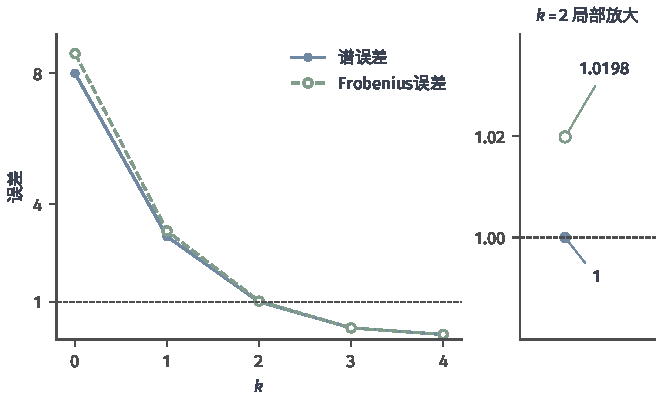
\includegraphics[width=112.0mm]{figures/01-mathematical-preliminaries-upper/02-linear-spaces/matplotlib/ch06-error-rank-curves/figure.pdf}
  \caption{固定奇异值$(8,3,1,0.2)$的最优误差曲线。给定横轴的秩可读出最低误差；
  给定水平误差阈值则寻找第一个满足要求的整数秩。$\tau=1$时，蓝色谱误差在
  $k=2$达标，绿色Frobenius误差要到$k=3$才达标。连线只辅助阅读，可行秩为整数。}
  \label{fig:ch06-error-rank-curves}
\end{figure}

\paragraph{中心化数据与PCA重构}

固定有限数据的重构是同一结论的实例。设$\bm X\in\mathbb R^{n\times d}$每行是一个样本，
先减去样本均值使每列之和为零。选择$\bm W^\top\bm W=\bm I_k$，低维坐标
$\bm Z=\bm X\bm W$，重构$\widehat{\bm X}=\bm Z\bm W^\top$，则
\begin{equation}
 \lVert\bm X-\bm X\bm W\bm W^\top\rVert_{\mathrm F}^2
 =\lVert\bm X\rVert_{\mathrm F}^2-\lVert\bm X\bm W\rVert_{\mathrm F}^2
 =\lVert\bm X\rVert_{\mathrm F}^2
 -\operatorname{tr}(\bm W^\top\bm X^\top\bm X\bm W).
 \label{eq:ls-pca-reconstruction}
\end{equation}
~\ref{sec:ls-quadratic-optimization}节的迹极值说明，最大化保留能量即取前$k$个右奇异
向量，重构恰为$\bm X_k$。这就是\term{主成分分析}（principal component analysis，PCA）
的有限矩阵形式；$n\geq2$时样本协方差$\bm X^\top\bm X/(n-1)$使保留方差总和为
$\lVert\bm X\bm W\rVert_{\mathrm F}^2/(n-1)$，最大化保留样本方差与最小化平方重构误差
等价。

例如四个中心化样本$(2,0)$、$(-2,0)$、$(0,1)$、$(0,-1)$，Gram矩阵为
$\operatorname{diag}(8,2)$。取$k=1$得$\bm W=(1,0)^\top$，坐标为$(2,-2,0,0)^\top$，
后两个样本都重构成零，误差平方为$2$。未中心化时，最强方向可能反映数据整体离原点的
位置而非围绕均值的变化；重构原始数据还应加回均值。把米改成毫米也会改变欧氏目标，是否
标准化必须由任务决定。最大样本方差不自动等于最有预测价值的方向，对总体协方差的估计
保证需要后续统计假设。

\paragraph{因子存储与作用代价}

以紧致因子存储$\bm A_k=\bm U_k\Sigma_k\bm V_k^\top$需要约$(m+n)k+k$个数，作用于一个
输入可先算$\bm V_k^\top\bm x$、按$\sigma_i$缩放、再乘$\bm U_k$。只有$k$相对两端
维数足够小时才真正节省存储和计算；小矩阵中因子开销可能更大。求SVD本身也有成本，不能
只统计后续乘法。噪声尺度若高于最后保留的奇异值，把$k$算得很精确也不等于方向可辨认，
方向可靠性由后续扰动分析章的谱隙条件判断。

\subsubsection{基于子空间压缩的近似求解}
\label{sec:ls-subspace-compression}

\paragraph{近似列空间与正交基}

完整SVD对超大矩阵代价过高。另一条路线把大矩阵近似拆成两步：先找一个$p$维近似列空间
$\operatorname{range}\bm Q$，$\bm Q\in\mathbb R^{m\times p}$满足
$\bm Q^\top\bm Q=\bm I_p$，$p\geq k$；再在这个小空间内解小规模问题。

\paragraph{压缩矩阵和小规模分解}

把$\bm A$投影到$\bm Q$上得到压缩矩阵$\bm C=\bm Q^\top\bm A\in\mathbb R^{p\times n}$，
对$\bm C$做薄SVD并截断到$k$项，$\bm C_k=\widehat{\bm U}_k\Sigma_k\widehat{\bm V}_k^\top$，
返回$\bm B=\bm Q\widehat{\bm U}_k\Sigma_k\widehat{\bm V}_k^\top$。大规模时只需要
$\bm Q$的乘法作用，不必显式形成完整$\bm U$。

\paragraph{子空间误差与截断误差的分离}

总误差由两部分独立组成：列空间未覆盖的残差$\lVert\bm A-\bm Q\bm Q^\top\bm A\rVert_2$，
加上压缩矩阵自身的截断尾能量。前者衡量找的子空间够不够大，后者衡量在子空间内保留几项，
两条预算分别分配，不能混为一谈。

\paragraph{随机化SVD的采样和计算流程}

\term{随机化SVD}（randomized SVD）只作为构造$\bm Q$的计算手段，本节给确定性流程，不给概率结论。取一个
$n\times p$的测试矩阵$\Omega$（元素独立抽样），计算$\bm Y=\bm A\Omega$，对$\bm Y$
作QR分解$\bm Y=\bm Q\bm R$得到正交基；随后压缩、小规模SVD、按上段返回候选。抽样把
寻找列空间的问题换成随机投影，成功概率与集中界由概率卷承担。

\paragraph{过采样、子空间迭代与访问次数}

$p=k+\ell$中$\ell$为过采样数，给弱方向留出余量。子空间迭代把$\bm Q$用
$(\bm A\bm A^\top)^q$刷新$q$次，每次需要正向与反向各访问$\bm A$一次，以访问次数
换取子空间精度；$q=0$就是单遍采样。过采样与迭代次数的选择依据概率卷的误差估计，
本节只记录流程与每步所需的矩阵作用。

\paragraph{Nyström的抽列与半正定重构}

半正定输入$\bm A\succeq0$另有\term{Nyström方法}（Nyström method）的抽列路径：按指标集$I$取出列块$\bm C=\bm A_{:,I}$与
交叉块$\bm W=\bm A_{I,I}$，用$\bm A\approx\bm C\bm W^{-1}\bm C^\top$重构，再对
$\bm C$作薄QR/SVD得到秩$k$候选。重构自动保持半正定；$\bm W$奇异时用伪逆或加小
扰动，属于数值实现细节。

\paragraph{确定性残差核验}

无论子空间如何得到，返回前都直接计算原矩阵残差
$\lVert\bm A-\bm B\rVert_{\mathrm F}$与子空间残差
$\lVert\bm A-\bm Q\bm Q^\top\bm A\rVert_2$，与既定预算比较；抽样随机性不改变核验
量，核验仍用原矩阵的确定性数值。

\paragraph{概率保证的后续入口}

期望误差、失败概率与集中不等式需要概率工具，可参考
\BookChapterRef{chap:probability-theory}{卷2《数学准备：概率、因果与决策》的概率基础章}；
本节只提供计算流程和确定性残差核验，不宣称随机子空间一定达到某条误差界。

\subsection{核范数惩罚的求解}
\label{sec:ls-nuclear-penalty-solve}

\paragraph{固定奇异值下的方向对齐}

回到~\eqref{eq:ls-nuclear-penalty-problem}。令$\bm B$的奇异值为$s_i\geq0$，展开
平方范数后方向只出现在交叉项$-\operatorname{tr}(\bm B^\top\bm A)$中。由
~\eqref{eq:ls-rearrangement-trace-bound}，固定$s_i$时令$\bm B$与$\bm A$的左右奇异
方向一致，交叉项最大、目标最小，方向子问题被方向对齐完全解决。

\paragraph{标量收缩与奇异值软阈值}

方向对齐后只剩逐个奇异值的独立问题
\begin{equation}
 \min_{s_i\geq0}\ \tfrac12(s_i-\sigma_i)^2+\lambda s_i.
 \label{eq:ls-soft-threshold-scalar}
\end{equation}
无约束极小点为$s_i=\sigma_i-\lambda$；若它小于零，非负约束把最优值压到$s_i=0$，故
\begin{equation}
 s_i=(\sigma_i-\lambda)_+=\max(\sigma_i-\lambda,0).
 \label{eq:ls-singular-value-soft-threshold}
\end{equation}
这是\term{奇异值软阈值}（singular value soft-thresholding）：保留方向上的奇异尺度被
$\lambda$整体压小，而不是像截断那样原值保留或整体舍弃。惩罚参数控制收缩幅度，产生的
实际秩取决于原谱，不等于直接指定$k$。

\paragraph{平衡因子表达与非凸求解边界}

核范数与因子平方惩罚之间有精确联系。
\begin{lemma}[核范数的因子分解表达]
\label{lem:matrix-analysis-nuclear-factorization}
设$\bm A\in\mathbb R^{m\times n}$，$r=\operatorname{rank}\bm A$。对任意正整数
$q\geq r$，
\begin{equation}
 \lVert\bm A\rVert_*
 =\min_{\substack{\bm L\in\mathbb R^{m\times q},\,
                  \bm R\in\mathbb R^{n\times q}\\
                  \bm L\bm R^\top=\bm A}}
   \tfrac12\bigl(\lVert\bm L\rVert_{\mathrm F}^2+\lVert\bm R\rVert_{\mathrm F}^2\bigr).
 \label{eq:matrix-analysis-nuclear-factorization}
\end{equation}
\end{lemma}
\begin{proof}
非零$\bm A$写紧致SVD$\bm P\Sigma\bm Q^\top$，取
$\bm L=\bm P\Sigma^{1/2}$、$\bm R=\bm Q\Sigma^{1/2}$，$q>r$补零列，两侧平方范数均为
$\sum_i\sigma_i$，故右侧不超过核范数。反过来令$\bm C=\bm P\bm Q^\top$，
$\lVert\bm C\rVert_2=1$，任意可行因子满足
$\lVert\bm A\rVert_*=\operatorname{tr}(\bm C^\top\bm A)
=\langle\bm C^\top\bm L,\bm R\rangle_{\mathrm F}
\leq\lVert\bm L\rVert_{\mathrm F}\lVert\bm R\rVert_{\mathrm F}
\leq\tfrac12(\lVert\bm L\rVert_{\mathrm F}^2+\lVert\bm R\rVert_{\mathrm F}^2)$，
依次使用Frobenius的Cauchy--Schwarz、混合次乘性与$2ab\leq a^2+b^2$。零矩阵取零因子。
\end{proof}
例如$\operatorname{diag}(4,1)$的平衡因子均为$\operatorname{diag}(2,1)$，每侧平方
能量$5$，平均后仍为核范数$5$；一侧乘$c$、另一侧除以$c$不改变乘积却一般增加总因子
能量，这就是“平衡”的含义。注意因子目标关于两侧联合变量仍非凸，恒等式不保证任意因子
算法达到全局最优；$q<r$时精确乘积约束不可行。
\section{张量低秩逼近}
\label{sec:ls-tensor-low-rank}

矩阵只有两个轴，SVD把它拆成两两配对的秩一项之和，并给出固定秩的全局最优。三个及以上
轴的\term{张量}（tensor，见~\ref{sec:ls-tensor-products}）有多种互不相同的“秩”概念，
矩阵截断SVD的最优性不能直接外推。本节先定义CP、Tucker与张量列车三种表示预算及其拟合
目标，再分别判断固定预算下最佳逼近是否存在，最后按模型给出只承担局部误差预算的求解
方法；全局非凸优化的一般理论留待后续最优化章。

\subsection{表示预算与目标}
\label{sec:ls-tensor-budget}

\subsubsection{CP表示}
\label{sec:ls-cp-representation}

\paragraph{多路分离的秩一张量}

一次读取同时依赖三组向量$\bm x\in\mathbb R^m$、$\bm y\in\mathbb R^n$、
$\bm z\in\mathbb R^p$时，完整参数数组需要$mnp$个数。取非零向量
$\bm a\in\mathbb R^m$、$\bm b\in\mathbb R^n$、$\bm c\in\mathbb R^p$，定义
\term{秩一张量}（rank-one tensor）
$(\bm a\otimes\bm b\otimes\bm c)_{i,j,k}=a_i b_j c_k$。有限求和可以分离：秩一读取等于
三个内积投影之积$(\bm a^\top\bm x)(\bm b^\top\bm y)(\bm c^\top\bm z)$，这一多路收缩
~\eqref{eq:linear-algebra-rank-one-contraction}已在5.11建立，
不必先生成$mnp$个乘积再读取，只需分别投影三组输入再乘三个标量。

\paragraph{秩一项之和与CP表示}

更丰富的参数写成若干可分离项之和，~\ref{sec:ls-tensor-products}节已引入
\term{CP表示}（CANDECOMP/PARAFAC representation）
\scite{math-kolda2009tensor}
\begin{equation}
 \mathcal W=\sum_{s=1}^r\bm a_s\otimes\bm b_s\otimes\bm c_s.
 \label{eq:ls-cp-sum}
\end{equation}
允许任意阶时按每条轴分别相乘；三阶是原型，更高阶逐条轴重复同一规则。

\paragraph{CP秩与因子规模}

能表示数组的最少非零秩一项数称为该标量域上的\term{张量秩}（tensor rank，CP秩），
零数组的秩取零。给出$r$项只说明秩至多为$r$，项之间可能相消；它与数组的轴数完全不同。
存储量从$mnp$变为$r(m+n+p)$，只有后者较小时才节省；小尺寸数组上因子参数反而更多。

\paragraph{因子缩放和排列的不唯一}

每一项内部可以把$\bm a_s$乘$c$、$\bm c_s$除以$c$而乘积不变，项的次序也可以任意
排列；与SVD不同，CP因子之间没有正交约束，同一数组的因子组不唯一，也不存在标准的
“左右奇异向量”。

\paragraph{CP预算下的拟合目标}

固定项数$r$，在所有CP秩不超过$r$的张量中最小化Frobenius距离：
\begin{equation}
 \min_{\{\bm a_s,\bm b_s,\bm c_s\}_{s=1}^r}
 \lVert\mathcal T-\sum_{s=1}^r\bm a_s\otimes\bm b_s\otimes\bm c_s\rVert_{\mathrm F}^2.
 \label{eq:ls-cp-fitting-objective}
\end{equation}
目标关于全体因子联合非凸，下面的交替方法只保证每步局部改进，不宣称全局最佳。

\subsubsection{Tucker表示}
\label{sec:ls-tucker-representation}

\paragraph{按轴展开与列空间}

Tucker模型不要求逐项分离，而是给每条轴各找一个子空间。把张量沿第$n$轴展开成矩阵
$\mathcal T_{(n)}\in\mathbb R^{I_n\times(\prod_{j\neq n}I_j)}$，其列空间就是第$n$
轴使用的方向集合。

\paragraph{各轴子空间与多线性秩}

第$n$个展开矩阵的秩$r_n=\operatorname{rank}\mathcal T_{(n)}$称为该轴的
\term{单秩}，元组$(r_1,\ldots,r_N)$为\term{多线性秩}（multilinear rank）。
它是各轴独立计数的，不需要各项跨轴配对。

\paragraph{基变换后的核心张量}

取各轴列空间的标准正交基$\bm U_n\in\mathbb R^{I_n\times r_n}$，经$n$模积把坐标
变换到基上，剩余的轴间耦合由\term{核心张量}（core tensor）
$\mathcal G\in\mathbb R^{r_1\times\cdots\times r_N}$记录，整体结构称
\term{Tucker表示}（Tucker decomposition）：
\begin{equation}
 \mathcal T\approx\mathcal G\times_1\bm U_1\times_2\cdots\times_N\bm U_N.
 \label{eq:ls-tucker-form}
\end{equation}

\paragraph{Tucker表示与参数规模}

参数规模为$\sum_n I_n r_n+\prod_n r_n$：各轴基向量加上核心。当$r_n\ll I_n$时比
稠密数组$\prod_n I_n$小得多，核心本身仍是小稠密数组。

\paragraph{多线性秩预算下的误差目标}

固定各轴上界$(k_1,\ldots,k_N)$，在$\operatorname{rank}\mathcal T_{(n)}\leq k_n$
的张量中最小化Frobenius距离。约束是各轴展开矩阵的秩条件，与CP的逐项分离条件不同。

\subsubsection{张量列车表示}
\label{sec:ls-tt-representation}

\paragraph{前后轴切分与矩阵展开}

\term{张量列车}（tensor train，TT）沿固定轴次序逐次切分：把前$j$条轴与其余轴分开，
把张量展开为矩阵$\mathcal T_{[1:j]}\in\mathbb R^{(\prod_{i\leq j}I_i)\times
(\prod_{i>j}I_i)}$，其秩记录这一切分需要多少连接指标。

\paragraph{逐次分解与中间连接指标}

$N$阶数组写成一串$N$个\term{TT核心}（TT core）
$\mathcal G^{(j)}\in\mathbb R^{r_{j-1}\times I_j\times r_j}$，相邻核心通过中间连接
指标$r_j$衔接，$r_0=r_N=1$。

\paragraph{TT核心与张量恢复}

逐元素恢复为
\begin{equation}
 t_{i_1\cdots i_N}
 =\sum_{a_1,\ldots,a_{N-1}}
 \mathcal G^{(1)}_{i_1,a_1}
 \mathcal G^{(2)}_{a_1,i_2,a_2}\cdots
 \mathcal G^{(N)}_{a_{N-1},i_N}.
 \label{eq:ls-tt-recovery}
\end{equation}

\paragraph{TT秩和轴次序}

$r_j$是第$j$个切分展开矩阵的秩，称为\term{TT秩}（TT rank）。它依赖轴次序：交换两条
轴可能改变所有$r_j$，选次序本身是一个预处理问题。

\paragraph{存储规模与拟合目标}

存储量为$\sum_j I_j r_{j-1}r_j$，避开了核心的全张量乘积；固定TT秩上界后最小化
Frobenius残差，求解方法见~\ref{sec:ls-tt-truncation}。

\subsection{存在性与选解}
\label{sec:ls-tensor-existence}

\paragraph{固定CP秩约束下的不取到现象}

与矩阵不同，集合$\{\mathcal W:\operatorname{rank}_{\mathrm{CP}}\mathcal W\leq r\}$
一般不是闭集：一串CP秩不超过$r$的张量可以收敛到CP秩$r+1$的极限，极限不在集合内。
因此固定$r$的最佳CP逼近可能只达到下确界而不取到，即最小距离不存在最小点；实张量上
这一现象真实发生，不能用“取极限”悄悄补上。需要存在性保证时应改用下面两类闭约束。

\paragraph{固定多线性秩上界与闭性}

条件$\operatorname{rank}\mathcal T_{(n)}\leq k_n$对每个$n$都是展开矩阵的
$(k_n+1)$阶子式同时为零，有限个矩阵秩条件的交是闭集。取有界极小化序列，由
~\ref{thm:ls-extreme-value}在闭有界集上取极限，最佳Tucker候选存在。

\paragraph{固定TT秩上界与闭性}

TT秩上界同样是有限个切分展开矩阵的秩条件，集合闭，最佳TT逼近存在；闭性来自矩阵秩条件，
不依赖逐项分离。

\paragraph{因子非唯一与逼近对象的非唯一}

即使逼近张量存在，因子也可能不唯一：CP有缩放与排列自由度，Tucker各轴基可右乘正交矩阵，
TT核心有 gauge 变换。弱谱条件下最佳逼近张量本身也可能不唯一，存在性结论不附带
唯一性保证。

\subsection{求解方法}
\label{sec:ls-tensor-solve}

\subsubsection{CP因子拟合}
\label{sec:ls-cp-alternating}

\paragraph{固定其他因子后的线性作用}

交替最小二乘每次只更新一条轴的因子。固定$\{\bm b_s,\bm c_s\}$，目标对
$\bm a_s$们线性：把指标$(j,k)$逐行排列，系数矩阵的第$s$列为
$\bm b_s\otimes\bm c_s$（Khatri--Rao列），待求向量由$\bm a_s$堆叠而成。

\paragraph{单因子最小二乘的构造}

这一步化为一个普通线性最小二乘问题，可直接使用~\ref{sec:ls-least-squares}节的正规
方程、QR或SVD工具求解，只替换待求因子，其他因子保持不变。

\paragraph{因子更新与循环次序}

按轴轮流更新：先解所有$\bm a_s$，再固定它们解$\bm b_s$，再解$\bm c_s$，循环往复；
每次更新后对列归一化并把尺度吸收到下一条轴，消除缩放自由度带来的漂移。

\paragraph{每步目标变化与停止}

每次单因子最小二乘都使平方残差不增，目标序列单调下降；以相对残差变化小于阈值或达到
轮数为停止条件。单调下降只说明不退步，不说明到达全局最小。

\paragraph{因子增大和数值退化}

因子列之间接近共线时，单因子正规方程病态，解被放大；归一化、列正交检查与必要时的
正则化属于数值实现，不能消除模型本身的非凸性。

\paragraph{局部停止与全局最优的区别}

停点只满足“固定其他因子时本条轴最优”的驻点条件，是局部极小；不同初值可能停在不同
驻点。全局最佳CP逼近的存在性与求解属于完整非凸优化理论，留待后续最优化章，本节不宣称
交替法给出全局解。

\subsubsection{Tucker截断}
\label{sec:ls-hosvd}

\paragraph{各轴展开的SVD}

对每个展开矩阵$\mathcal T_{(n)}$做SVD，取前$k_n$个左奇异向量组成$\bm U_n$，
这一步复用~\ref{thm:ls-svd-existence}，不重新构造SVD。

\paragraph{主子空间选择与核心计算}

核心由投影得到$\mathcal G=\mathcal T\times_1\bm U_1^\top\cdots\times_N\bm U_N^\top$，
各轴独立选取主子空间。

\paragraph{截断张量的重构}

截断候选$\widetilde{\mathcal T}
=\mathcal G\times_1\bm U_1\cdots\times_N\bm U_N$，即\term{HOSVD}（higher-order SVD，高阶SVD）截断。

\paragraph{各轴误差与总误差界}

第$n$轴舍弃的展开能量为$\sum_{i>k_n}\sigma_i(\mathcal T_{(n)})^2$；总Frobenius
误差平方被各轴舍弃能量之和控制：
\begin{equation}
 \lVert\mathcal T-\widetilde{\mathcal T}\rVert_{\mathrm F}^2
 \leq\sum_{n=1}^N\sum_{i>k_n}\sigma_i(\mathcal T_{(n)})^2.
 \label{eq:ls-hosvd-error-bound}
\end{equation}
这是各轴独立截断的累计预算，不是联合最优误差。

\paragraph{秩预算与存储代价}

按各轴尾能量分别选定$k_n$，再核对参数规模$\sum_n I_n k_n+\prod_n k_n$是否落在
预算内；核心随$\prod_n k_n$增长，维数较多时核心本身可能成为瓶颈。

\paragraph{HOSVD的非最优边界}

各轴子空间独立选取，没有联合最小化总残差，因此HOSVD截断不保证达到固定多线性秩下的
全局最佳；迭代修正各轴基可以改善残差，但仍是局部改进，不改变非最优边界。

\subsubsection{张量列车截断}
\label{sec:ls-tt-truncation}

\paragraph{轴顺序与首次展开}

先固定轴次序，把第$1$轴与其余轴分开展开为矩阵，做SVD并按$r_1$截断。

\paragraph{截断SVD与首个TT核心}

薄SVD给出左因子与缩放，前者整理为首个TT核心$\mathcal G^{(1)}$，右因子矩阵传给下一步。

\paragraph{余因子传递与逐次展开}

把余因子矩阵沿第$2$轴再次切分、SVD、截断，得到$\mathcal G^{(2)}$并继续传递；逐次
进行到最后一条轴，每个切分复用矩阵截断SVD的尾能量结论。

\paragraph{局部误差的累计控制}

每一步截断都引入一个尾能量，总误差平方不超过各步尾能量之和，误差沿链条累计而非抵消。

\paragraph{总误差预算的逐步分配}

把总预算$\tau^2$分配到各步$\tau_j^2$，$\sum_j\tau_j^2\leq\tau^2$，每步只在
自身预算内截断；预算分配影响各$r_j$的大小。

\paragraph{TT秩与中间存储}

记录每步$r_j$与中间矩阵尺寸，避免连接指标无节制增长；中间存储随
$\prod_{i\leq j}I_i$与$r_j$变化，是TT实现的主要开销。

\paragraph{重构残差与非最优边界}

由核心按~\eqref{eq:ls-tt-recovery}重构后直接计算残差$\lVert\mathcal X-\widehat{\mathcal X}\rVert_{\mathrm F}$，
并与各次局部尾能量之和比较；逐次贪心截断不联合最优，局部误差累计得到的是预算保证而非最佳值，
残差超出预算时应回退上一层连接秩而不是继续贪心。

\subsection{结果核验}
\label{sec:ls-tensor-verification}

\paragraph{重构残差与表示规模}

返回候选前分别计算Frobenius重构残差$\lVert\mathcal X-\widehat{\mathcal X}\rVert_{\mathrm F}$
与实际参数量，与原定预算逐项比较。三套口径的计数不同，不能共用一个总数：CP为
$R\sum_{i=1}^d n_i$；Tucker为$\sum_{i=1}^d n_i r_i+\prod_{i=1}^d r_i$；TT为
$\sum_{i=1}^d n_i r_{i-1}r_i$（约定$r_0=r_d=1$）。预算通常同时给定残差上界$\varepsilon$
与参数量上界$N$，两项都满足才算交差；例如$n_i=100$、$d=4$、$R=10$时CP需$4000$个数，
而同维满张量为$10^8$，压缩比由计数直接算出，不能只凭"低秩"宣称节省。

\paragraph{因子增大、数值退化与停止}

交替法每轮记录残差序列$\rho_t=\lVert\mathcal X-\widehat{\mathcal X}^{(t)}\rVert_{\mathrm F}$
与轮数$t$；同时检查因子列范数是否失控（归一化后单列能量占比畸高）、相邻因子是否近似共线
（$\bm a_r^{(i)\top}\bm a_{r+1}^{(i)}/(\lVert\bm a_r^{(i)}\rVert\lVert\bm a_{r+1}^{(i)}\rVert)$
接近$1$）。当$\rho_t-\rho_{t-1}<\delta\,\rho_{t-1}$或达到轮数上限即停，停点只作为局部结果
报告，不写成全局最佳；退化发生时应重新初始化或降低$R$，而不是把局部残差当最优误差。
\section{正交映射逼近}
\label{sec:ls-orthogonal-approximation}

第~\ref{sec:ls-matrix-low-rank}节限制候选的秩，本节限制候选的几何性质：要求它保持长度。
有噪声的坐标变换可能不再是旋转，任务是在所有保持长度的矩阵中找一个离它最近的，包括
方阵正交、矩形部分等距与定向（行列式为正）三种约束。方向配对不等式在本节直接复用，
不重新证明。

\subsection{目标与约束}
\label{sec:ls-orthogonal-objective}

\paragraph{最近正交矩阵与对应点对齐}

给定$\bm A\in\mathbb R^{d\times d}$，在正交矩阵中最小化Frobenius距离
\begin{equation}
 \min_{\bm R^\top\bm R=\bm I_d}\ \lVert\bm A-\bm R\rVert_{\mathrm F}^2.
 \label{eq:ls-nearest-orthogonal-objective}
\end{equation}
形状对齐中更常见的是两组已对应列向量$\bm X,\bm Y\in\mathbb R^{d\times n}$，求
$\bm R$使$\lVert\bm R\bm X-\bm Y\rVert_{\mathrm F}^2$最小，即\term{正交Procrustes问题}
（orthogonal Procrustes problem）。

\paragraph{列正交、正交与定向约束}

$\bm Q\in\mathbb R^{m\times n}$（$m\geq n$）只要求$\bm Q^\top\bm Q=\bm I_n$，
称为列正交或\term{部分等距}（partial isometry），它在$\mathbb R^n$上保持长度但
$\mathbb R^m$维数有余量；方阵$\bm R^\top\bm R=\bm I$同时给出$\bm R\bm R^\top=\bm I$。
定向约束再加$\det\bm R=1$，候选限于特殊正交群$\mathrm{SO}(d)$，排除反射。

\paragraph{输入误差尺度与目标矩阵}

默认用Frobenius距离，它把每条输出方向的偏差平方累计；谱范数口径下最优解可能不唯一，
见~\ref{sec:ls-orthogonal-existence}。$\bm A$可以奇异，奇异方向留有的自由度正是
非唯一性的来源。

\subsection{存在性与唯一性}
\label{sec:ls-orthogonal-existence}

\paragraph{维数条件与可行性}

列正交要求$m\geq n$；$m<n$时不存在$\bm Q^\top\bm Q=\bm I_n$，问题不可行，应改求
$\bm Q\bm Q^\top=\bm I_m$的行正交版本。方阵正交与$\mathrm{SO}(d)$对任意$d$非空。

\paragraph{有限维闭有界约束与极值存在}

正交集合由$\bm R^\top\bm R=\bm I$定义，是有限维中的闭有界集（各列单位长度且互相
正交），Frobenius距离连续，由~\ref{thm:ls-extreme-value}最小点存在；$\mathrm{SO}(d)$
是其闭子集，同样存在最小点。

\paragraph{秩亏、奇异值与非唯一性}

$\bm A$有零奇异值或重复弱奇异值时，规范部分等距因子在零方向上不受原矩阵约束，最优
矩阵可能不唯一。例如$\operatorname{diag}(2,0)$的规范因子$\bm Q=\operatorname{diag}(1,0)$，
而正交延拓$\operatorname{diag}(1,1)$与$\operatorname{diag}(1,-1)$乘以同一半正定
因子都给原矩阵；延拓自由不等于规范因子本身不唯一。

\subsection{求解方法}
\label{sec:ls-orthogonal-solve}

\subsubsection{基于SVD的直接求解}
\label{sec:ls-orthogonal-svd}

\paragraph{距离目标的迹配对展开}

展开平方距离：
\begin{equation}
 \lVert\bm A-\bm R\rVert_{\mathrm F}^2
 =\lVert\bm A\rVert_{\mathrm F}^2+d-2\operatorname{tr}(\bm R^\top\bm A),
 \label{eq:ls-orthogonal-trace-expand}
\end{equation}
前两项与$\bm R$无关，故最小误差等价于最大化$\operatorname{tr}(\bm R^\top\bm A)$。

\paragraph{SVD方向对齐与极因子}

设$\bm A=\bm U\Sigma\bm V^\top$，令$\bm W=\bm U^\top\bm R\bm V$，则$\bm W$正交，
$\operatorname{tr}(\bm R^\top\bm A)=\operatorname{tr}(\bm W\Sigma)$。由
~\eqref{eq:ls-rearrangement-trace-bound}，配对上界为$\sum_i\sigma_i$，在
$\bm W=\bm I$即$\bm R=\bm U\bm V^\top$时取等。这一因子就是\term{极分解}
（polar decomposition）\label{def:matrix-analysis-polar-decomposition}
$\bm A=\bm Q\bm H$的规范部分：
\begin{equation}
 \bm A=\bm Q\bm H,\qquad
 \bm H=(\bm A^\top\bm A)^{1/2}=\bm V\Sigma\bm V^\top\succeq0,\qquad
 \bm Q=\bm U\bm V^\top.
 \label{eq:matrix-analysis-polar-decomposition}
\end{equation}
$\bm H$由唯一半正定平方根确定，$\bm Q$在$\operatorname{range}\bm H$上被
$\bm A=\bm Q\bm H$确定，在其正交补取零，故规范$\bm Q$唯一。

\paragraph{矩形部分等距与正交延拓}

$m>n$或秩亏时，规范$\bm Q=\bm U_r\bm V_r^\top$只在$(\ker\bm A)^\perp$上保持长度，
并在$\ker\bm A$上取零；把它延拓为整个空间的正交矩阵需要任选零方向的标准正交基，
延拓不唯一。迭代趋于规范部分等距，并不自动给出任意正交延拓。

\paragraph{对应点对齐的Procrustes化简}

对齐$\lVert\bm R\bm X-\bm Y\rVert_{\mathrm F}^2$展开为
$\lVert\bm Y\rVert_{\mathrm F}^2+\lVert\bm X\rVert_{\mathrm F}^2
-2\operatorname{tr}(\bm R^\top\bm Y\bm X^\top)$，对$\bm M=\bm Y\bm X^\top$
作SVD$\bm M=\widehat{\bm U}\widehat\Sigma\widehat{\bm V}^\top$，同一配对论证给
$\bm R_*=\widehat{\bm U}\widehat{\bm V}^\top$。若还允许平移，先减去各组均值
$\bar{\bm x},\bar{\bm y}$，求得$\bm R_*$后取
$\bm t_*=\bar{\bm y}-\bm R_*\bar{\bm x}$。

\paragraph{定向约束下的符号修正}

限制$\det\bm R=1$时，令$s=\det(\bm U\bm V^\top)\in\{-1,1\}$。$s=1$直接取
$\bm R=\bm U\bm V^\top$；$s=-1$时实正交矩阵至少有一个特征值$-1$，其余特征值实部
不超过$1$，故$\operatorname{tr}\bm W\leq d-2$，把最小奇异值方向的符号翻转即可达到
\label{sec:linear-algebra-orthogonal-procrustes}：
\begin{equation}
 \bm R_*=\bm U\operatorname{diag}(1,\ldots,1,s)\bm V^\top
 \in\argmin_{\bm R\in\mathrm{SO}(d)}\lVert\bm A-\bm R\rVert_{\mathrm F}.
 \label{eq:linear-algebra-nearest-rotation}
\end{equation}
行列式修正应放在最小奇异值方向，而不是任意改一列。例如$\bm A=\operatorname{diag}(2,1,-1/2)$
的最近正交矩阵为$\operatorname{diag}(1,1,-1)$，但它是反射；限制为旋转后上式给
$\bm R_*=\bm I$，平方误差$1+(3/2)^2=13/4$。定向限制确实增加误差，不能称作无代价
的修正\scite{math-lawrence2019kabsch}。

\paragraph{最优性与非唯一边界}

严格奇异值间隙使规范因子唯一；零奇异值或等奇异值留下自由度，最优矩阵不唯一。谱范数口径
下即使有间隙也可能多个最优，与~\ref{sec:ls-low-rank-existence}的结论一致。

\subsubsection{基于乘法迭代的近似求解}
\label{sec:ls-polar-iteration}

\paragraph{极因子的乘法近似需求}

完整SVD代价较高；只需要极因子时，可以构造只用矩阵乘法的多项式更新，避免显式分解。

\paragraph{Newton--Schulz多项式更新}

对标量缩放到$\lVert\bm A\rVert_2\leq1$附近的$\bm X_0=\bm A/\beta$，固定更新
\begin{equation}
 \bm X_{t+1}=\tfrac12\bm X_t(3\bm I-\bm X_t^\top\bm X_t).
 \label{eq:ls-newton-schulz-polar}
\end{equation}
它的不动点满足$\bm X^\top\bm X=\bm I$（矩形时为部分等距），与逆迭代的多项式校正
同一类构造，收敛域与二次递推证明在~\ref{sec:ls-matrix-function-iteration-convergence}
节完成。

\paragraph{奇异方向保持与尺度变化}

更新与$\bm A$共用右奇异方向，对每个奇异值$s$化为标量递推
$s_{t+1}=\tfrac12s_t(3-s_t^2)$；$0<s<\sqrt3$时它把$s$推向$1$，零方向保持零，
方向不发生混合。

\paragraph{输入缩放与初始区间}

取$\beta\geq\lVert\bm A\rVert_2$（例如$\beta=\lVert\bm A\rVert_{\mathrm F}$）把谱
压到可检查区间，初始化无需分解；超出区间会使标量映射发散，不能省略缩放。

\paragraph{零方向与部分等距输出}

零奇异方向在迭代中保持零，极限是规范部分等距；迭代不供应任意正交延拓，需要延拓时另行
补基。

\paragraph{有限步整形与极限求解的区别}

有限次迭代只得到近似极因子，不是精确解；每步三次矩阵乘法，停止量为正交残差
$\lVert\bm X_t^\top\bm X_t-\bm I\rVert$，与极限方程$\bm X^\top\bm X=\bm I$分开评价。
标量递推在$s_t$接近$1$时二次收敛，残差平方量级下降，故达到给定容限所需步数与初始
距离有关，不能用固定步数代替收敛判断。

\subsection{结果核验}
\label{sec:ls-orthogonal-verification}

\paragraph{正交残差与部分等距残差}

方阵核验$\lVert\bm R^\top\bm R-\bm I\rVert$；矩形候选核验
$\lVert\bm Q^\top\bm Q-\bm I_n\rVert$与$\bm Q\bm Q^\top$是否等于目标投影。
定向约束再检查$\det\bm R=1$。

\paragraph{作用误差、目标差与计算代价}

同时计算目标差$\lVert\bm A-\bm R\rVert_{\mathrm F}^2=\sum_i(\sigma_i-1)^2$并与该理论
最小值比较，两者之差即方向未对齐的代价。点对问题再把$\lVert\bm A\bm R-\bm B\rVert_{\mathrm F}$
与$\lVert\bm B\rVert_{\mathrm F}$归一，得到可解释的对齐比例。乘法迭代记录每步矩阵乘法次数，
与完整SVD的$O(mn\min(m,n))$建立代价按规模比较；迭代收敛到什么精度也由残差
$\lVert\bm X^\top\bm X-\bm I\rVert$的截断水平决定，不写成精确等于极因子。
\section{对称与谱约束逼近}
\label{sec:ls-symmetric-spectral-approximation}

~\ref{sec:ls-orthogonal-approximation}节的正交集合不是凸集，最优解可能不唯一；本节处理
三类凸约束：最近对称矩阵、最近半正定矩阵与谱范数球内的最近矩阵。凸集合上的平方距离
有唯一最小点，求解归结为对称化、特征值截断与奇异值裁剪。

\subsection{目标与约束}
\label{sec:ls-symmetric-objective}

\paragraph{最近对称矩阵与最近半正定矩阵}

给定$\bm A\in\mathbb R^{d\times d}$，第一类在对称矩阵集合
$\operatorname{Sym}_d=\{\bm S:\bm S=\bm S^\top\}$中找最近点；第二类\term{最近半正定矩阵}
（nearest positive semidefinite matrix）在半正定锥
$\mathbb S_+^d=\{\bm P:\bm P=\bm P^\top,\ \bm x^\top\bm P\bm x\geq0\ \forall\bm x\}$
中找最近点，误差均取Frobenius平方距离。

\paragraph{谱范数球与Frobenius距离}

第三类约束把候选限制在\term{谱范数球}（spectral norm ball）$\{\bm B:\lVert\bm B\rVert_2\leq\rho\}$内，
$\rho>0$，同样最小化$\lVert\bm A-\bm B\rVert_{\mathrm F}^2$。它限制的是最大奇异值，
与对称约束限制特征值符号是两类问题。

\subsection{存在性与唯一性}
\label{sec:ls-symmetric-existence}

\paragraph{闭凸约束与平方距离的唯一最小点}

对称集合是线性子空间，半正定锥与谱范数球是凸集：两对称矩阵的线段仍对称；两个半正定
矩阵的凸组合$(1-t)\bm P+t\bm Q$仍半正定；谱范数是范数，单位球凸。平方距离
$\lVert\bm A-\bm B\rVert_{\mathrm F}^2$是严格凸函数，凸集上的最小点唯一。可行集闭，
极小化序列有界（谱球直接有界；半正定锥上最近点满足$\lVert\bm P\rVert_{\mathrm F}
\leq\lVert\bm A\rVert_{\mathrm F}$，故序列有界），由~\ref{thm:ls-extreme-value}
取到极值。

\paragraph{特征值约束与奇异值约束的区别}

对称与半正定问题在实对称谱坐标中求解，使用~\ref{thm:ls-real-symmetric-spectral}的
特征值；谱范数球问题使用奇异值。前者方向被限制在输入自己的特征向量上，后者允许两端
方向分别配对，不能把特征值截断直接套到非对称输入。

\subsection{求解方法}
\label{sec:ls-symmetric-solve}

\subsubsection{对称与半正定约束}
\label{sec:ls-psd-projection}

\paragraph{对称部分与反对称部分}

任意$\bm A$唯一分解为对称部分与反对称部分：
\begin{equation}
 \bm A_{\mathrm s}=\tfrac12(\bm A+\bm A^\top),\qquad
 \bm A_{\mathrm k}=\tfrac12(\bm A-\bm A^\top),
 \qquad \bm A=\bm A_{\mathrm s}+\bm A_{\mathrm k}.
 \label{eq:ls-skew-split}
\end{equation}

\paragraph{Frobenius误差的正交分离}

反对称矩阵与对称矩阵在Frobenius配对下正交：
$\operatorname{tr}(\bm A_{\mathrm k}^\top\bm A_{\mathrm s})=0$，故对任意对称$\bm S$，
\begin{equation}
 \lVert\bm A-\bm S\rVert_{\mathrm F}^2
 =\lVert\bm A_{\mathrm k}\rVert_{\mathrm F}^2
 +\lVert\bm A_{\mathrm s}-\bm S\rVert_{\mathrm F}^2.
 \label{eq:ls-symmetric-orthogonal-separation}
\end{equation}
第一项与$\bm S$无关。

\paragraph{最近对称矩阵}

第二项在$\bm S=\bm A_{\mathrm s}$时为零，故最近对称矩阵就是对称部分
$\bm S_*=\tfrac12(\bm A+\bm A^\top)$，反对称分量$\bm A_{\mathrm k}$无法由对称候选
消除，全部计入误差。

\paragraph{半正定约束下的谱坐标}

对半正定问题，先取$\bm A_{\mathrm s}$的实对称谱分解
$\bm A_{\mathrm s}=\bm Q\Lambda\bm Q^\top$，$\Lambda=\operatorname{diag}(\lambda_i)$。
在谱坐标中对称候选$\bm S=\bm Q\operatorname{diag}(\mu_i)\bm Q^\top$，半正定要求
$\mu_i\geq0$，误差平方为$\sum_i(\lambda_i-\mu_i)^2$，各$\mu_i$独立。

\paragraph{特征值非负截断}

每个标量问题$\min_{\mu_i\geq0}(\lambda_i-\mu_i)^2$的解为$\mu_i=\max(\lambda_i,0)$，
故
\begin{equation}
 \bm P_*=\bm Q\operatorname{diag}(\lambda_1^+,\ldots,\lambda_d^+)\bm Q^\top,
 \qquad \lambda_i^+=\max(\lambda_i,0).
 \label{eq:ls-nearest-psd}
\end{equation}
负特征值截为零而不是取绝对值，因为半正定只要求非负，把负号翻正会改变方向配对并增大
距离。

\paragraph{可行性与最优性核验}

核验$\bm P_*\succeq0$（所有$\mu_i\geq0$）与残差$\lVert\bm A-\bm P_*\rVert_{\mathrm F}$；
例如$\bm A=\operatorname{diag}(2,-1)$的最近半正定矩阵为$\operatorname{diag}(2,0)$，
误差平方为$1$，而$\operatorname{diag}(2,1)$不是可行点且距离更大。

\subsubsection{谱范数约束}
\label{sec:ls-spectral-ball}

\paragraph{谱范数球与奇异值上界}

$\lVert\bm B\rVert_2\leq\rho$等价于$\bm B$的每个奇异值$s_i\leq\rho$，由
~\ref{thm:ls-svd-existence}的奇异值定义直接得到。

\paragraph{迹配对与最优方向}

展开$\lVert\bm A-\bm B\rVert_{\mathrm F}^2$，方向只出现在交叉项
$-\operatorname{tr}(\bm B^\top\bm A)$。由~\eqref{eq:ls-rearrangement-trace-bound}，
固定奇异值时让$\bm B$与$\bm A$使用相同左右奇异方向最优。

\paragraph{标量区间上的最近值}

方向对齐后，每个奇异值独立求解
$\min_{0\leq s_i\leq\rho}(s_i-\sigma_i)^2$，解为
$s_i=\min(\sigma_i,\rho)$：$\sigma_i<\rho$时保留原值，超过$\rho$的压到边界。

\paragraph{奇异值裁剪与矩阵恢复}

设$\bm A=\bm U\Sigma\bm V^\top$，返回
\begin{equation}
 \bm B_*=\bm U\operatorname{diag}(\min(\sigma_1,\rho),\ldots,
 \min(\sigma_q,\rho))\bm V^\top.
 \label{eq:ls-spectral-clipping}
\end{equation}

\paragraph{最优性与边界核验}

核验$\lVert\bm B_*\rVert_2\leq\rho$与残差$\lVert\bm A-\bm B_*\rVert_{\mathrm F}^2
=\sum_i(\sigma_i-\min(\sigma_i,\rho))^2$；落在边界上的方向$s_i=\rho$对应被裁剪的
大奇异值，内部方向$s_i=\sigma_i<\rho$保持原值，两者不要混淆。例如$\sigma=(3,1)$、
$\rho=2$时裁剪为$(2,1)$，残差平方为$(3-2)^2=1$，第二个奇异值未被改动。

\subsection{结果核验}
\label{sec:ls-symmetric-verification}

\paragraph{可行性残差与逼近误差}

分别核对约束条件：对称差$\lVert\bm S-\bm S^\top\rVert_{\mathrm F}$、半正定特征值下界
$\min_i\lambda_i(\bm P)\geq0$、谱范数上界$\lVert\bm B\rVert_2\leq\rho$，再报告Frobenius
逼近误差。三类误差分开列：可行性残差应在数值精度内为零，逼近误差才是与$\bm A$的距离；
可行性不满足时误差数字没有意义。例如把$\bm A=\operatorname{diag}(2,-1)$投影到半正定锥，
$\bm P_*=\operatorname{diag}(2,0)$，可行性残差为零而逼近误差平方恰为$(-1)^2=1$，
二者不可合并成一个数。

\paragraph{正交集合与凸谱约束的区别}

正交Stiefel集合非凸（~\ref{sec:ls-orthogonal-approximation}），可能多解；本节三类
集合凸，解唯一。一般凸投影理论、不等式约束优化与次梯度方法留待后续最优化章，这里只解
当前三个具体问题。
\section{矩阵方程}
\label{sec:ls-matrix-equations}
\label{sec:linear-algebra-matrix-equations}

前面各节的未知量是向量或约束矩阵，本节未知量本身是一张矩阵：左乘对未知矩阵的各行作线性
组合，右乘对各列作线性组合。先建立矩阵上的线性作用与相容、可逆条件，再用向量化与实Schur
块求解；本章只作代数判据、对称结构和正定结果核验，不使用长期衰减定理构造正定解。

\subsection{方程与线性算子}
\label{sec:ls-matrix-equation-types}

\paragraph{单侧、双侧与多项矩阵作用}

单侧方程$\bm A\bm X=\bm C$只从左边作用；$\bm X\bm B=\bm C$只从右边作用；双侧
$\bm A\bm X\bm B=\bm C$两端同时约束。多项作用的典型是\term{Sylvester方程}
（Sylvester equation）
\begin{equation}
 \bm A\bm Z+\bm Z\bm B=\bm C,
 \label{def:matrix-analysis-sylvester-equation}
\end{equation}
给定$\bm A\in\mathbb R^{m\times m}$、$\bm B\in\mathbb R^{n\times n}$、
$\bm C\in\mathbb R^{m\times n}$，求$\bm Z\in\mathbb R^{m\times n}$。固定作用矩阵后，
这些方程关于未知矩阵都是线性的。

\paragraph{向量化与Kronecker表示}

~\ref{sec:ls-kronecker-products}节的向量化恒等式
$\operatorname{vec}(\bm A\bm X\bm B)
=(\bm B^\top\otimes\bm A)\operatorname{vec}\bm X$把矩阵方程编码为普通向量方程；
Sylvester方程向量化为
\begin{equation}
 (\bm I_n\otimes\bm A+\bm B^\top\otimes\bm I_m)\operatorname{vec}\bm Z
 =\operatorname{vec}\bm C.
 \label{eq:ls-sylvester-vectorized}
\end{equation}
向量系统的求解方法可以直接复用，但大规模时应利用左右乘法，避免存储$mn\times mn$的
Kronecker矩阵。

\paragraph{Sylvester与Lyapunov方程}

\term{Lyapunov方程}是Sylvester的对称特化：连续型
$\bm A\bm P+\bm P\bm A^\top=\bm W$，离散型
$\bm A^\top\bm P\bm A-\bm P=\bm Q$，右端$\bm W,\bm Q$对称半正定，未知量要求对称。
它的代数可逆性与对称性在本节判断；由系统衰减构造正定解的构造不属于本章。

\subsection{存在性与唯一性}
\label{sec:ls-matrix-equation-existence}

\paragraph{单侧与双侧方程的相容性}

$\bm A\bm X=\bm C$相容当且仅当$\bm C$的每一列都在$\operatorname{range}\bm A$内，
即$\operatorname{rank}[\bm A\ \bm C]=\operatorname{rank}\bm A$。$\bm A\bm X\bm B=\bm C$
相容要求$\bm C$落在$\bm A$的列空间经右作用可达的范围内，用秩条件
$\operatorname{rank}\bm A+\operatorname{rank}\bm B$与$\operatorname{rank}\bm C$
比较判断，不能在秩亏时直接相乘两个逆。

\paragraph{Kronecker算子的可逆性}

Sylvester算子$\mathcal L(\bm Z)=\bm A\bm Z+\bm Z\bm B$可逆当且仅当
\begin{equation}
 \lambda_i(\bm A)+\lambda_j(\bm B)\neq0
 \quad\text{对所有 }i,j,
 \qquad
 \operatorname{spec}(\bm A)\cap\operatorname{spec}(-\bm B)=\varnothing.
 \label{eq:ch06-sylvester-spectral-separation}
\end{equation}
实矩阵的复共轭特征值成对出现，条件按全体特征值计数。充分性由~\ref{sec:ls-sylvester-schur}
的回代直接给出；必要性来自排序后线性系统为三角系统，其行列式是全部
$\lambda_i(\bm A)+\lambda_j(\bm B)$的乘积，出现零因子则算子奇异。例如标量方程
$2z+(-2)z=c$在$c\neq0$时无解，$c=0$时解不唯一。条件不要求$\bm A,\bm B$各自可逆：
$\bm A=\bm0,\bm B=\bm I$仍唯一可解。

对角情形把条件看得最直接。设$\bm A$与$\bm B$都是对角矩阵，对角元分别为
$a_{i,i}$与$b_{j,j}$，方程$\bm A\bm Z+\bm Z\bm B=\bm C$按元素解耦，
第$(i,j)$个方程为$(a_{i,i}+b_{j,j})z_{i,j}=c_{i,j}$，闭式解
\begin{equation}
 z_{i,j}=\frac{c_{i,j}}{a_{i,i}+b_{j,j}}.
 \label{eq:ls-sylvester-diagonal-closed-form}
\end{equation}
只要每个分母$a_{i,i}+b_{j,j}$非零就唯一可解；某一对和为零，该位置方程退化为
$0\cdot z_{i,j}=c_{i,j}$，$c_{i,j}\neq0$时无解、$c_{i,j}=0$时该位置自由，正是谱分离
条件在对角基上的翻版。

\paragraph{Lyapunov算子的可逆性与解的对称性}

若$\bm W$对称且算子可逆，Sylvester解$\bm P$自动对称：$\bm P-\bm P^\top$落在齐次
算子的核中，可逆时核为零，故$\bm P=\bm P^\top$，这是代数结论，不依赖稳定性。
所得解是否正定是有限计算问题：对候选$\bm P$作Cholesky分解成功即核验
$\bm P\succ0$，不需要先证明系统衰减。

\subsection{求解方法}
\label{sec:ls-matrix-equation-solve}

\subsubsection{单侧与双侧方程}
\label{sec:ls-one-sided-two-sided}

\paragraph{单侧方程的逐列求解}

$\bm A\bm X=\bm C$是$n$个共享系数矩阵的多右端问题，分解一次（~\ref{sec:ls-direct-methods}
的三角分解或~\ref{sec:ls-pseudoinverse}的SVD）复用于每一列，不存在列间耦合。

\paragraph{双侧作用的可达方向}

$\bm A\bm X\bm B=\bm C$中，左作用限制输出列空间，右作用限制输入组合方向；先按
~\ref{sec:ls-matrix-equation-existence}的秩条件确认可达，再谈求解。

\paragraph{可逆两端的逐侧求解}

$\bm A,\bm B$都可逆时，混合乘积规则给出
$(\bm A\otimes\bm B)^{-1}=\bm A^{-1}\otimes\bm B^{-1}$，逐侧反演得
$\bm X=\bm A^{-1}\bm C\bm B^{-1}$；显式求逆只在两端可逆时成立。

\paragraph{秩亏情形的全部解}

一端或两端秩亏时，取伪逆特解再加各自零空间的任意方向；全部解由特解与齐次解相加给出，
最小范数特解由~\ref{sec:ls-pseudoinverse}构造。

\paragraph{不相容时的最小二乘目标}

不相容时等式无精确解，改求$\min_{\bm X}\lVert\bm A\bm X\bm B-\bm C\rVert_{\mathrm F}^2$。
向量化后系数矩阵为$\bm B^\top\otimes\bm A$，这是普通最小二乘正规方程问题，复用
~\ref{sec:ls-least-squares}的法方程与伪逆工具；注意此时报告的是最小残差而非零残差，
可行性缺口（$\operatorname{rank}$条件差）仍须单独说明。

\paragraph{原矩阵方程的残差核验}

无论是否向量化求解，返回前都直接在原矩阵尺度计算残差$\bm A\bm X\bm B-\bm C$及其
Frobenius范数，不把Kronecker向量在浮点截断下的数值残差当作矩阵残差；双侧方程还要分别
核验左、右作用后是否落在可达子空间。向量化系统的条件数与原矩阵尺度的关系留到第7章扰动分析。

\subsubsection{Sylvester方程}
\label{sec:ls-sylvester-schur}

\paragraph{两侧正交变换与方程保持}

分别取$\bm A=\bm Q\bm T\bm Q^\top$、$\bm B=\bm U\bm S\bm U^\top$的正交相似，令
$\bm Y=\bm Q^\top\bm Z\bm U$、$\bm D=\bm Q^\top\bm C\bm U$，方程化为
\begin{equation}
 \bm T\bm Y+\bm Y\bm S=\bm D.
 \label{eq:ls-sylvester-transformed}
\end{equation}
正交相似保持谱分离条件与Frobenius残差，方程形式不变。

\paragraph{实不变子空间与Schur块}

实矩阵的正交相似可化为实准上三角Schur形：对角块为$1\times1$实特征值或$2\times2$
实块（对应一对共轭复特征值），严格上三角。本节只使用这一形式作代数回代，QR迭代的
收敛证明留给~\ref{sec:ls-matrix-function-iteration-convergence}节。

\paragraph{Hessenberg约化与实移位QR}

构造上先用Householder双边把$\bm A,\bm B$约化为上Hessenberg形（次对角线以下为零），
再用隐式实移位QR迭代把次对角线小元素消去，得到准上三角块；约化与迭代只产生Schur形式，
不承担收敛速度与移位选择的结论，那些由~\ref{sec:ls-matrix-function-iteration-convergence}
节处理。

\paragraph{准三角块上的约化方程}

按块逐元写出
\begin{equation}
 (\bm T_{i,i}+\bm S_{j,j})\bm Y_{i,j}
 =\bm D_{i,j}-\sum_{k>i}\bm T_{i,k}\bm Y_{k,j}
          -\sum_{\ell<j}\bm Y_{i,\ell}\bm S_{\ell,j},
 \label{eq:ls-sylvester-block-recurrence}
\end{equation}
右侧所需元素已按次序算出：准上三角使$\bm T_{i,k}$只在$k>i$非零、$\bm S_{\ell,j}$只在
$\ell<j$非零，故按$i$自下而上、$j$自左向右的次序，求和项引用的$\bm Y$块均已求出，
每块只解一个小线性系统而不回到完整Kronecker方程。

\paragraph{一阶、二阶块的递推求解}

$1\times1$块直接除以$t_{ii}+s_{jj}$；$2\times2$实块对解一个$2\times2$线性系统，
系数由$\bm T_{i,i}\otimes\bm I+\bm I\otimes\bm S_{j,j}$给出，可逆条件已由谱分离
保证。按列从左向右、每列自下向上计算。

\paragraph{原坐标恢复与残差}

$\bm Z=\bm Q\bm Y\bm U^\top$恢复原坐标，直接在原基核验$\bm A\bm Z+\bm Z\bm B-\bm C$
的Frobenius范数；Schur坐标中的块残差只用于定位递推错误，最终验收必须回到原矩阵等式。

\paragraph{分解复用与计算代价}

$\bm A,\bm B$的Schur分解只建立一次，多个右端$\bm C$复用同一回代；总代价为$O(m^3+n^3)$
加回代，远小于形成$mn\times mn$Kronecker矩阵。

\subsubsection{Lyapunov方程}
\label{sec:ls-lyapunov}

\paragraph{连续型与离散型的作用区别}

连续型$\bm A\bm P+\bm P\bm A^\top=\bm W$是Sylvester取$\bm B=\bm A^\top$、
$\bm C=\bm W$；离散型$\bm A^\top\bm P\bm A-\bm P=\bm Q$是二次作用，系数块关系
不同，不能套用同一回代方向。

\paragraph{实Schur坐标中的约化方程}

对$\bm A$取实Schur形$\bm A=\bm Q\bm T\bm Q^\top$，连续型在$\bm Y=\bm Q^\top\bm P\bm Q$
坐标中化为$\bm T\bm Y+\bm Y\bm T^\top=\bm Q^\top\bm W\bm Q$，按块递推；离散型
同理变换后逐块求解。

\paragraph{对称未知量与块求解}

利用$\bm P=\bm P^\top$只求解上三角块，未知量从$d^2$个减到$d(d+1)/2$个；对角块由
对称方程直接给出，上三角块解出后下三角由转置复制，对称块关系由递推自然保持，不需要
额外施加对称约束。

\paragraph{解的恢复与对称性核验}

$\bm P=\bm Q\bm Y\bm Q^\top$恢复后核验$\lVert\bm P-\bm P^\top\rVert_{\mathrm F}$在容限
内为零；若不对称，说明块递推时把下三角块也当成自由变量更新了，应只沿上三角填值并回代。

\paragraph{正定性核验与代数唯一性}

可逆条件满足时解唯一；候选$\bm P\succ0$由Cholesky分解成功（$\bm P=\bm L\bm L^\top$、
$\bm L$对角元为正）核验，这是有限代数计算。本章只判断给定解是否正定，不证明“右端半正定
加稳定性推出正定解”，那是另一套级数或积分构造。

\paragraph{稳定性构造的后续入口}

离散型正定解的矩阵级数构造在~\ref{sec:ls-matrix-series-exponential}节由稳定传播
给出；连续型的积分构造与稳定性等价定理由微积分之后的微分方程章承担，本章不能借作前提。
\section{本章小结}
\label{sec:ls-equations-summary}

本章把“在给定空间里求一个满足方程或目标的对象”组织成一条共同路线：先写出目标与约束，
再判断最小点是否存在、是否唯一，随后选择直接法或迭代法求解，最后用可计算的残差核验
候选。~\ref{sec:ls-subspace-nearest-points}节在仿射子空间上求最近点，把正交投影建立为
线性问题的原型；~\ref{sec:ls-exact-linear-equations}节处理相容线性方程组，给出消元、
三角分解等直接法与分裂迭代法，回答“解存在、唯一还是有自由度”；
~\ref{sec:ls-least-squares}节把不相容目标转为残差最小，SVD、伪逆与正规方程给出全部最优
解；~\ref{sec:ls-quadratic-optimization}节在对称矩阵上用特征值与迹极值挑选最优方向，
建立方向选择的一般工具。

~\ref{sec:ls-matrix-low-rank}节在固定秩预算下求最佳低秩矩阵，Eckart--Young--Mirsky定理
说明截断SVD同时最小化谱误差与Frobenius误差，核范数惩罚则把方向对齐化为逐奇异值软阈值；
~\ref{sec:ls-tensor-low-rank}节指出张量有CP、多线性、TT等不同秩概念，CP秩集合不闭、
最佳逼近可能不取到，Tucker与TT借矩阵秩条件保证闭性，各自方法只承担局部误差预算；
~\ref{sec:ls-orthogonal-approximation}节在非凸的正交约束下用SVD方向对齐求最近正交
矩阵，定向修正翻转最小奇异值方向；~\ref{sec:ls-symmetric-spectral-approximation}节在凸
的对称、半正定与谱范数约束下得到唯一解，分别对应对称化、特征值非负截断与奇异值裁剪；
~\ref{sec:ls-matrix-equations}节用向量化与实Schur块求解单侧、双侧、Sylvester与
Lyapunov方程，可逆性由谱分离条件判断，正定结果用Cholesky核验。

贯穿全章的判据有三条：存在性依赖可行集闭与极小化序列有界，唯一性依赖间隙、凸性或
谱分离条件，可行性必须先于优化判断。方向配对不等式在最佳低秩逼近、最近正交矩阵与谱范数
裁剪中反复复用，说明这三个表面不同的问题在固定奇异值后是同一个标量选择问题。可计算
不等于准确：直接法的条件数、迭代法的停止量、子空间与抽样的误差预算都需要数值核验，
速度与敏感性的定量分析由下一章承担。


\chapter{分析}
\label{chap:linear-analysis}
\label{chap:matrix-analysis}

第~\ref{chap:linear-representation}章规定了对象怎样用基与坐标记录，第~\ref{chap:linear-operations}章规定了对象之间怎样运算，第~\ref{chap:linear-equations-and-optimization}章规定了未知量满足什么条件、怎样求得。这些讨论都默认输入是精确的、运算只做一次。实际测量总有误差，数据在机器上只能有限精度表示，而许多任务还要把同一个作用反复施加。本章回答两个彼此独立的问题：输入或计算稍有改变时，一次任务的答案会变多少（\ref{sec:ls-perturbation}）；同一个规则反复作用时，序列趋向哪里、以什么速度趋向（\ref{sec:ls-convergence}）。前者是扰动分析，后者是收敛分析，二者使用的证据不能互相替代。

扰动分析固定一个已经定义好的任务（求逆、解方程、最小二乘、读谱值与方向、计算矩阵函数），把输入的微小增量送到输出端，测量最坏情况下的放大倍数。它先约定比较哪个输出、用什么范数、允许改变哪些分量，再给出绝对误差与相对误差的界；问题本身对输入敏感，与算法是否算错是两件事，必须分开归因。收敛分析则让近似序列或矩阵幂随步数演化，研究极限是否存在、误差按什么速率衰减，以及持续噪声把精度压到什么下限。

这两件事不能用同一个数字概括。条件数衡量一次输入增量的瞬时放大，不回答反复作用的长期结果：$2\bm I$ 与 $\bm I/2$ 的二范数条件数都是 $1$，前者的幂逐次增长、后者的幂逐次衰减；非正规矩阵还可能在最初几步先放大误差，之后再衰减。因此本章先用扰动界刻画单点敏感度，再在收敛部分处理长期传播，第~\ref{sec:ls-analysis-summary}节把两类证据汇总。

\section{扰动分析}
\label{sec:ls-perturbation}
\label{sec:linear-algebra-stability}
\label{sec:matrix-analysis-conditioning-perturbation}

前面各章在精确输入上建立了运算、求解与逼近。本节固定一个任务，回答一个更实际的问题：
交给算法的数据与理想输入相差一点时，答案会相差多少。\term{扰动}（perturbation）指
允许范围内的输入增量，扰动分析不改变任务本身，只测量输入增量被放大多少。先在
\ref{sec:ls-perturbation-conditioning}统一误差尺度与条件数，再依次估计基本运算、
方程解、最小二乘、谱值与子空间、矩阵函数的响应，最后把问题本身的敏感度与算法的
舍入误差分开（\ref{sec:ls-numerical-stability}）。每个结论都要写清所用范数、允许
改变的分量、秩或谱隙条件以及定义域边界；没有这些条件的“误差小”没有意义。

\subsection{扰动与条件数}
\label{sec:ls-perturbation-conditioning}

\subsubsection{输入、输出与误差}

\paragraph{固定运算与输入输出}

扰动分析的第一步是把任务固定下来：给定映射 $F$、理想输入 $\bm z$ 和明确的输出
$F(\bm z)$，再问 $\bm z$ 改变后 $F(\bm z)$ 改变多少。这里只改变数据，不更换算法；
“算法算错了”是另一项误差，在\ref{sec:ls-numerical-stability}节单独处理。任务不同，
比较的输出也不同：求逆比较逆矩阵，解方程比较解向量，最小二乘要分别比较系数、拟合值
与残差，谱分解要分别比较谱值与子空间。先指定输出对象，后面的误差尺度才有附着点。

\paragraph{输入增量和输出增量}

设实际输入为 $\bm z+\Delta\bm z$，其中 $\Delta\bm z$ 是输入增量，输出增量定义为
\[
 \Delta\bm y=F(\bm z+\Delta\bm z)-F(\bm z).
\]
对线性任务 $F(\bm z)=\bm A\bm z$，输出增量就是 $\Delta\bm y=\bm A\,\Delta\bm z$，
与理想输入 $\bm z$ 本身无关；对非线性任务，$\Delta\bm y$ 还通过 $F$ 依赖 $\bm z$。
扰动分析只比较两个输出的差，不要求写出 $F$ 的完整表达式。

\paragraph{绝对误差与相对误差}

绝对误差直接取增量范数 $\lVert\Delta\bm z\rVert$、$\lVert\Delta\bm y\rVert$；当输入
与输出本身有尺度时，更常用\term{相对误差}（relative error）
\[
 \frac{\lVert\Delta\bm z\rVert}{\lVert\bm z\rVert},
 \qquad
 \frac{\lVert\Delta\bm y\rVert}{\lVert F(\bm z)\rVert}.
\]
相对误差对整体缩放不变：把所有数据乘以 $10^3$，绝对误差同步放大，相对误差不变，
因此它反映“变化占原有量的比例”。\term{绝对误差}（absolute error）则保留实际大小，
在输出接近零时必须使用。

\paragraph{零输入或零输出的尺度边界}

分母为零时相对误差没有定义：$\bm z=\bm0$ 时不能除以 $\lVert\bm z\rVert$，
$F(\bm z)=\bm0$ 时不能除以 $\lVert F(\bm z)\rVert$。此时报告绝对误差，或改用任务
指定的参考尺度（如矩阵范数 $\lVert\bm A\rVert$）。秩变化等不连续处也不能套用
“小输入产生小输出”的微分式判断，伪逆在秩改变处的跳变见\ref{sec:ls-ordinary-ls-sensitivity}。

\paragraph{范数选择与结构约束}

误差大小依赖所选范数，同一增量在 $\ell_1$、$\ell_2$、Frobenius 范数下数值不同，
比较前必须写明口径。还要写明允许改变哪些分量：只改右端、同时改矩阵与右端、要求
扰动矩阵保持对称，得到的敏感度不同。例如只允许右端变化的方程，与允许系数矩阵
一起变化的方程，不是同一个扰动问题。

\subsubsection{条件数}

\paragraph{有限增量的局部放大比}

对固定任务 $F$，输入增量 $\Delta\bm z$ 引起的输出增量 $\Delta\bm y$，其放大比为
$\lVert\Delta\bm y\rVert/\lVert\Delta\bm z\rVert$。扰动分析取足够小的允许增量，观察
这个比值在局部的上界；它是有限增量的比值，不预先使用导数。

\paragraph{允许扰动中的最坏方向}

输入增量可以朝任意允许方向取，敏感度由最坏方向决定：
\[
 \sup_{\Delta\bm z\neq0}
 \frac{\lVert F(\bm z+\Delta\bm z)-F(\bm z)\rVert}
      {\lVert\Delta\bm z\rVert}.
\]
对线性作用 $\bm x\mapsto\bm A\bm x$，这个上确界就是第~\ref{sec:ls-matrix-norms}节
建立的诱导范数 $\lVert\bm A\rVert$，在最大放大方向达到；它不描述某一个具体扰动，
而描述所有允许扰动中最不利的那个。

\paragraph{绝对条件数}

任务 $F$ 在 $\bm z$ 处的\term{绝对条件数}（absolute condition number）定义为
局部放大比的上确界；线性作用 $\bm A$ 的绝对条件数就是 $\lVert\bm A\rVert$。
绝对条件数带单位，随整体缩放改变，适合零输入或零输出的场合。

\paragraph{相对尺度与相对条件数}

把输入、输出都换成相对尺度，得到\term{相对条件数}（relative condition number）
\[
 \kappa_{\mathrm{rel}}(F;\bm z)
 =\sup_{\Delta\bm z\neq0}
 \frac{\lVert\Delta\bm y\rVert/\lVert F(\bm z)\rVert}
      {\lVert\Delta\bm z\rVert/\lVert\bm z\rVert}.
\]
对线性作用 $\bm x\mapsto\bm A\bm x$（$\bm x\neq\bm0$），
\[
 \kappa_{\mathrm{rel}}(\bm A;\bm x)
 =\frac{\lVert\bm A\rVert\,\lVert\bm x\rVert}{\lVert\bm A\bm x\rVert},
\]
它随方向变化：落在被压缩方向上的 $\bm x$ 放大比大，落在主伸缩方向上则小。

\paragraph{矩阵作用和求逆的不同敏感度}

对可逆方阵 $\bm A$，求逆任务 $\bm y\mapsto\bm A^{-1}\bm y$ 在所有方向上的最坏
相对条件数为
\begin{equation}
 \kappa(\bm A)=\lVert\bm A\rVert\,\lVert\bm A^{-1}\rVert,
 \label{eq:matrix-analysis-condition-number}
\end{equation}
它与作用任务在单个 $\bm x$ 处的相对条件数不是同一个量。欧氏范数下由SVD
（\ref{sec:ls-svd}）给出
\begin{equation}
 \kappa_2(\bm A)=\frac{\sigma_{\max}(\bm A)}{\sigma_{\min}(\bm A)}.
 \label{eq:matrix-analysis-spectral-condition-number}
\end{equation}
$\lVert\bm I\rVert=1$ 与次乘性保证 $\kappa(\bm A)\geq1$；正交矩阵 $\kappa_2=1$，
接近奇异时 $\sigma_{\min}\to0$，$\kappa_2$ 增大。同一个 $\bm A$，沿某个特定右端
作用可能很稳，求逆或反求系数却可能很敏感，因此矩阵没有一个包办所有任务的
“通用条件数”。

\begin{definition}[可逆矩阵的条件数]
\label{def:matrix-analysis-condition-number}
对同一向量范数诱导的矩阵范数，可逆方阵 $\bm A$ 的条件数为式
~\eqref{eq:matrix-analysis-condition-number}。它记录求逆任务的最坏相对放大，
不直接等于作用在某个具体右端上的放大比。
\end{definition}

\paragraph{条件数的适用范围与最坏界}

条件数是最坏方向上的上界，不是每个扰动都达到的倍数；它控制足够小的局部扰动，
有限扰动还要保留到奇异边界的余量（\ref{sec:ls-inverse-sensitivity}）。条件数
回答“一次输入增量被放大多少”，不回答反复作用的长期增长或衰减，后者属收敛分析。

\subsection{基本运算的敏感度}
\label{sec:ls-basic-operations-sensitivity}

本节用增量展开估计第~\ref{sec:ls-operations-summary}节各基本运算的响应，不重复
运算定义与计算教程。范数口径默认与输入输出一致，未注明处使用诱导范数或
Frobenius 范数。

\subsubsection{加法与乘法}

\paragraph{加减运算的增量恒等式}

两个输入分别改变：$(\bm x+\Delta\bm x)\pm(\bm y+\Delta\bm y)
-(\bm x\pm\bm y)=\Delta\bm x\pm\Delta\bm y$，故
\[
 \lVert\Delta(\bm x\pm\bm y)\rVert
 \leq\lVert\Delta\bm x\rVert+\lVert\Delta\bm y\rVert.
\]
加法本身不放大误差，两项误差按三角不等式相加；输出大小不进入这个绝对界。

\paragraph{输入抵消与相对误差}

当 $\bm x\approx-\bm y$ 时，理想输出 $\bm x+\bm y$ 很小，两项的绝对误差不变，
相对误差 $\lVert\Delta\bm x+\Delta\bm y\rVert/\lVert\bm x+\bm y\rVert$ 却被小分母
放大。例如 $x=1.0001$、$y=-1.0000$，各带 $5\times10^{-5}$ 的绝对误差，理想和为
$10^{-4}$，相对误差可达 $1$ 量级。抵消不是算法失误，而是小输出使相对尺度失效，
此时应报告绝对误差。

\paragraph{矩阵作用的输入增量}

系数矩阵固定、右端改变时，$\Delta(\bm A\bm x)=\bm A\,\Delta\bm x$，故
$\lVert\Delta(\bm A\bm x)\rVert\leq\lVert\bm A\rVert\lVert\Delta\bm x\rVert$。
正向作用的绝对放大由诱导范数控制，与 $\bm x$ 无关。

\paragraph{算子范数与最大放大方向}

最坏方向上 $\lVert\bm A\Delta\bm x\rVert/\lVert\Delta\bm x\rVert$ 达到
$\lVert\bm A\rVert$；欧氏范数下即最大奇异值 $\sigma_{\max}$。反方向
（由输出反求输入）才除以 $\sigma_{\min}$，那是求逆任务的事。

\paragraph{两侧矩阵扰动与交叉项}

两个因子都改变时，
\[
 (\bm A+\Delta\bm A)(\bm x+\Delta\bm x)-\bm A\bm x
 =\bm A\,\Delta\bm x+\Delta\bm A\,\bm x+\Delta\bm A\,\Delta\bm x.
\]
前两项分别是固定矩阵对另一侧增量的响应，最后一项是两个增量的乘积，在小扰动下
为二阶量。矩阵乘积同理：
$(\bm A+\bm E)(\bm B+\bm F)-\bm A\bm B
=\bm A\bm F+\bm E\bm B+\bm E\bm F$。

\paragraph{乘积误差的尺度与边界}

取相容范数，
\[
 \lVert(\bm A+\bm E)(\bm B+\bm F)-\bm A\bm B\rVert
 \leq\lVert\bm A\rVert\lVert\bm F\rVert
 +\lVert\bm E\rVert\lVert\bm B\rVert
 +\lVert\bm E\rVert\lVert\bm F\rVert.
\]
相对形式把各项除以 $\lVert\bm A\bm B\rVert$，大因子本身会放大另一侧的误差；
二阶项 $\lVert\bm E\rVert\lVert\bm F\rVert$ 在 $\lVert\bm E\rVert,\lVert\bm F\rVert$
足够小时可略去。逐项乘法（Hadamard）每个位置独立，误差按位置相乘，不跨位置求和。

\subsubsection{配对与度量}

\paragraph{内积的两侧增量}

$\langle\bm x,\bm y\rangle$ 两侧分别改变：
\[
 \Delta\langle\bm x,\bm y\rangle
 =\langle\Delta\bm x,\bm y\rangle+\langle\bm x,\Delta\bm y\rangle
 +\langle\Delta\bm x,\Delta\bm y\rangle.
\]
由 Cauchy--Schwarz（\ref{sec:ls-inner-products}），一阶项不超过
$\lVert\bm y\rVert\lVert\Delta\bm x\rVert
+\lVert\bm x\rVert\lVert\Delta\bm y\rVert$，末项为二阶。

\paragraph{近正交与小配对值}

理想内积 $\langle\bm x,\bm y\rangle\approx0$ 时，扰动项 $\langle\Delta\bm x,\bm y\rangle$
相对于近零的配对值可能很大，相对误差无意义。此时几何关系（是否正交）由投影分量
判断，配对数值本身只报告绝对变化。

\paragraph{权重变化与正定性保持}

加权配对 $\langle\bm M\bm x,\bm y\rangle$ 中加权矩阵 $\bm M$ 也改变。$\bm M$ 对称
正定时，若 $\lVert\bm M^{-1/2}\Delta\bm M\,\bm M^{-1/2}\rVert_2<1$，扰动后仍
正定：对任意 $\bm v$，
$\bm v^\top(\bm M+\Delta\bm M)\bm v
=\lVert\bm M^{1/2}\bm v\rVert^2
+\bm v^\top\Delta\bm M\bm v>0$。正定余量不足时先失去正定性，再谈配对误差。

\paragraph{加权配对的联合误差}

联合展开
\[
\Delta(\langle\bm M\bm x,\bm y\rangle)
=\langle\Delta\bm M\,\bm x,\bm y\rangle
+\langle\bm M\Delta\bm x,\bm y\rangle
+\langle\bm M\bm x,\Delta\bm y\rangle
+\text{二阶项},
\]
三项分别由加权矩阵、第一输入、第二输入的变化贡献，加权矩阵误差还乘以 $\lVert\bm x\rVert$，
大输入会放大加权矩阵误差。

\paragraph{范数的反三角不等式}

范数本身对输入扰动绝对稳定：由三角不等式的反向形式，
\[
 \big|\lVert\bm x+\Delta\bm x\rVert-\lVert\bm x\rVert\big|
 \leq\lVert\Delta\bm x\rVert.
\]
长度读数不会因为方向转动而剧烈变化；相对误差只在 $\bm x$ 接近零时需要小心。

\paragraph{距离的绝对界与相对尺度}

距离 $d(\bm x,\bm y)=\lVert\bm x-\bm y\rVert$ 满足
\[
 d(\bm x+\Delta\bm x,\bm y+\Delta\bm y)
 \leq d(\bm x,\bm y)+\lVert\Delta\bm x\rVert+\lVert\Delta\bm y\rVert.
\]
两点几乎重合时理想距离接近零，相对距离改用绝对距离或任务参考尺度报告。

\subsubsection{重排与张量运算}

\paragraph{重排与系数误差的对应}

转置、轴置换、reshape（\ref{sec:ls-reshaping}）只改变索引记录，不改动元素。
系数误差随位置一一对应搬到新数组，不产生新的求和或抵消，逐项范数误差原样保留。

\paragraph{保持的范数与改变的矩阵尺度}

置换保持 Frobenius 范数与逐项 $\ell_2$ 误差；但同一组元素从向量改成矩阵后，诱导
矩阵范数改变，因此“作为变换的放大能力”改变，尽管元素一个未动。重排不制造误差，
只改变后续口径下的尺度读数。

\paragraph{张量积的因子增量展开}

$(\bm A+\bm E)\otimes(\bm B+\bm F)-\bm A\otimes\bm B
=\bm E\otimes\bm B+\bm A\otimes\bm F+\bm E\otimes\bm F$。
张量积范数满足 $\lVert\bm A\otimes\bm B\rVert=\lVert\bm A\rVert\lVert\bm B\rVert$，
故一阶界为 $\lVert\bm E\rVert\lVert\bm B\rVert
+\lVert\bm A\rVert\lVert\bm F\rVert$。

\paragraph{Kronecker作用的放大界}

Kronecker 积作用在向量化矩阵上（\ref{sec:ls-kronecker-products}），
$\lVert(\bm A\otimes\bm B)\operatorname{vec}\bm X\rVert
\leq\lVert\bm A\rVert\lVert\bm B\rVert\lVert\bm X\rVert$；两侧因子的条件数
相乘进入放大，不能只看其中一个。

\paragraph{缩约求和中的权重传播}

缩约 $\sum_i x_i y_i$（\ref{sec:ls-tensor-contraction}）对每个因子分别线性，
但求和把多项误差累加：绝对误差不超过各项误差绝对值之和，项数越多累计越大。

\paragraph{抵消与输出相对误差}

求和中大小相近、符号相反的项抵消后输出很小，各项的累计绝对误差相对输出被放大；
迹（见下一小节）就是对角项的缩约，同样遵守这条边界。

\subsubsection{迹与行列式}

\paragraph{迹的增量与对角误差}

$\operatorname{tr}(\bm A+\bm E)-\operatorname{tr}\bm A
=\operatorname{tr}\bm E=\sum_i e_{i,i}$，故
$|\operatorname{tr}\bm E|\leq\sum_i|e_{i,i}|
\leq\sqrt r\,\lVert\bm E\rVert_{\mathrm F}$（$r$ 为阶数）。迹只读取对角项，
非对角误差不进入结果。

\paragraph{对角抵消与相对读取误差}

对角元素符号相反、大小相近时，理想迹接近零，对角误差之和相对迹被放大。迹是
标量读取量，矩阵本身可能完全正常，只是这个读数不适合用相对误差评价。

\paragraph{行列式的多线性增量展开}

行列式对每一列多线性（\ref{sec:ls-determinant-properties}）。把 $\bm A+\bm E$ 的
各列依次替换，一阶展开为
\[
 \det(\bm A+\bm E)-\det\bm A
 =\sum_{i=1}^d\det[\bm a_1,\dots,\bm e_i,\dots,\bm a_d]
 +O(\lVert\bm E\rVert^2),
\]
高阶项同时替换两列以上，是二阶及以上量。

\paragraph{单列变化与高阶交叉项}

只改第 $i$ 列时，差值等于该列余子式乘 $e_i$；多列同时改变产生交叉项。一阶界按
各列余子式求和估计，不把所有扰动塞进单一比值。

\paragraph{近奇异矩阵的体积敏感度}

$|\det\bm A|=\prod_i\sigma_i$（Gram 体积）。对角例子 $\bm A=\operatorname{diag}(1,\varepsilon)$，
$\det\bm A=\varepsilon$，第二对角元改变 $\delta\varepsilon$ 时相对变化为
$|\delta\varepsilon|/\varepsilon$；$\varepsilon\to0$ 时体积读数对微小变化
无限敏感，这是接近奇异的直接表现。

\paragraph{零行列式处的绝对误差}

$\det\bm A=0$ 时相对误差无定义，只报告绝对变化 $|\det(\bm A+\bm E)|$；
秩从 $0$ 变为非零属于不连续边界，不能用局部界外推。

\subsection{方程解的敏感度}
\label{sec:ls-equation-sensitivity}

\subsubsection{逆矩阵}
\label{sec:ls-inverse-sensitivity}
\label{sec:ch06-inverse-stability}

\paragraph{最小奇异值与输入下界}

$\bm A$ 可逆时，SVD（\ref{sec:ls-svd}）给出 $\lVert\bm A\bm x\rVert_2\geq\sigma_{\min}(\bm A)\lVert\bm x\rVert_2$，
因而 $\lVert\bm A^{-1}\rVert_2=1/\sigma_{\min}(\bm A)$。最小奇异值越小，逆对任意
输入的放大越大，这是求逆敏感度的根源。

\paragraph{扰动后的下界与可逆邻域}

设 $\bm B=\bm A+\bm E$。若 $\lVert\bm A^{-1}\bm E\rVert<1$，则 $\bm B$ 可逆：
假设 $\bm B\bm x=\bm0$，则 $\bm A\bm x=-\bm E\bm x$，左乘 $\bm A^{-1}$ 得
$\bm x=-\bm A^{-1}\bm E\bm x$，取范数有
$\lVert\bm x\rVert\leq\lVert\bm A^{-1}\bm E\rVert\lVert\bm x\rVert$，
与 $\bm x\neq\bm0$ 矛盾。这是有限增量的直接论证，不借助展开级数。

\paragraph{逆矩阵差的恒等式}

由 $\bm B\bm B^{-1}=\bm A\bm A^{-1}=\bm I$ 直接整理，
\begin{equation}
 \bm B^{-1}-\bm A^{-1}
 =-\bm B^{-1}\bm E\,\bm A^{-1},
 \label{eq:ch06-inverse-finite-perturbation}
\end{equation}
这是精确恒等式，不含高阶余项；差分被夹在两个逆之间。

\paragraph{逆差的绝对误差界}

从恒等式取范数，
$\lVert\bm B^{-1}-\bm A^{-1}\rVert
\leq\lVert\bm B^{-1}\rVert\lVert\bm E\rVert\lVert\bm A^{-1}\rVert$。
估计 $\bm B^{-1}$：由 $\bm B\bm x=\bm y$ 得
$\bm x=\bm A^{-1}(\bm y-\bm E\bm x)$，故
\[
 \lVert\bm x\rVert
 \leq\frac{\lVert\bm A^{-1}\rVert}{1-\lVert\bm A^{-1}\bm E\rVert}
 \lVert\bm y\rVert,
\]
即 $\lVert\bm B^{-1}\rVert
\leq\lVert\bm A^{-1}\rVert/(1-\lVert\bm A^{-1}\bm E\rVert)$。

\paragraph{相对误差与条件数}

代入恒等式，相对逆差满足
\[
 \frac{\lVert\bm B^{-1}-\bm A^{-1}\rVert}
      {\lVert\bm A^{-1}\rVert}
 \leq
 \frac{\kappa(\bm A)\,\lVert\bm E\rVert/\lVert\bm A\rVert}
      {1-\kappa(\bm A)\,\lVert\bm E\rVert/\lVert\bm A\rVert},
\]
分子是条件数乘相对扰动，分母保留到奇异边界的余量。

\paragraph{接近奇异边界的放大}

令 $\alpha=\kappa(\bm A)\lVert\bm E\rVert/\lVert\bm A\rVert$。$\alpha$ 越接近 $1$，
分母越小，逆差急剧放大；$\alpha\geq1$ 只表示本界失效、可逆性未被保证，
不等于 $\bm B$ 一定奇异。对角例子 $\bm A=\operatorname{diag}(1,\varepsilon)$，
$\kappa_2=1/\varepsilon$，相对扰动 $\delta$ 放大到 $\delta/(\varepsilon-\delta)$，
$\varepsilon\to0$ 时边界无限接近。

\subsubsection{线性方程}
\label{sec:ls-linear-system-sensitivity}

\paragraph{固定系数下的右端扰动}

$\bm A$ 固定、右端由 $\bm b$ 变为 $\bm b+\Delta\bm b$，由
$\bm A(\bm x+\Delta\bm x)=\bm b+\Delta\bm b$ 得 $\Delta\bm x=\bm A^{-1}\Delta\bm b$，
故
\[
 \lVert\Delta\bm x\rVert\leq\lVert\bm A^{-1}\rVert\lVert\Delta\bm b\rVert.
\]
绝对误差只受逆范数控制；相对形式为
\[
 \frac{\lVert\Delta\bm x\rVert}{\lVert\bm x\rVert}
 \leq\kappa(\bm A)\frac{\lVert\Delta\bm b\rVert}{\lVert\bm b\rVert}.
\]

\paragraph{奇异方向与解误差放大}

小奇异值方向把右端误差放大 $1/\sigma_{\min}$ 倍。两个 $2\times2$ 例子对照。
良态情形取 $\bm A_1=\begin{smallmatrix}2&0\\0&1\end{smallmatrix}$，
$\kappa_2=2$；右端由 $\bm b_1=(2,1)^\top$ 改为 $\bm b_1'=(2,1.01)^\top$，
解由 $(1,1)^\top$ 变为 $(1,1.01)^\top$：右端相对变化 $0.01/\sqrt5\approx0.00447$，
解的相对变化 $0.01/\sqrt2\approx0.00707$，放大比约 $1.58$，不超过 $\kappa_2=2$。
近平行情形取 $\bm A_2=\begin{smallmatrix}1&1\\0&\varepsilon\end{smallmatrix}$
（$\varepsilon>0$ 很小），两列接近同向，其最小奇异值约为 $\varepsilon/\sqrt2$、
$\kappa_2\approx2/\varepsilon$。取 $\varepsilon=10^{-2}$、右端 $\bm b=(1,0)^\top$，
解为 $\bm x=(1,0)^\top$；只把第二分量改动 $\eta=10^{-2}$ 得 $\bm b'=(1,\eta)^\top$，
由 $\varepsilon x_2=\eta$ 与 $x_1+x_2=1$ 得 $x_2=1$、$x_1=0$，解由 $(1,0)^\top$
跳到 $(0,1)^\top$：右端相对变化仅 $\eta=10^{-2}$，解的相对变化却为 $\sqrt2$，
放大比约 $\sqrt2/\eta\approx141$，与 $\kappa_2\approx2/\varepsilon=200$ 同量级。
系数矩阵接近平行的方向，其系数对观测误差高度敏感；两个例子都不含浮点误差，
差别完全来自问题本身。

\paragraph{系数和右端的联合扰动}

$\bm A+\bm E$、$\bm b+\Delta\bm b$ 同时改变，$\bm x+\Delta\bm x$ 满足
$(\bm A+\bm E)(\bm x+\Delta\bm x)=\bm b+\Delta\bm b$，减去理想方程
$\bm A\bm x=\bm b$，得到解差方程
\[
 \bm A\,\Delta\bm x=\Delta\bm b-\bm E\bm x-\bm E\Delta\bm x.
\]

\paragraph{解差方程与误差界}

把 $\bm E\Delta\bm x$ 移到左侧并整理，
\begin{equation}
 \frac{\lVert\Delta\bm x\rVert}{\lVert\bm x\rVert}
 \leq
 \frac{\kappa(\bm A)}{1-\kappa(\bm A)\lVert\bm E\rVert/\lVert\bm A\rVert}
 \left(
 \frac{\lVert\Delta\bm b\rVert}{\lVert\bm b\rVert}
 +\frac{\lVert\bm E\rVert}{\lVert\bm A\rVert}
 \right).
 \label{eq:matrix-analysis-linear-system-perturbation}
\end{equation}
右端扰动与系数扰动先相加，再被条件数放大，最后除以余量。

\paragraph{条件数和最坏相对误差}

式~\eqref{eq:matrix-analysis-linear-system-perturbation} 是最坏方向上的上界，
一般右端不一定达到；实际解差还与 $\Delta\bm b$、$\bm E$ 是否落在放大方向有关。
条件数给出天花板，不给出每个具体扰动的精确倍数。

\paragraph{有限扰动的可逆条件}

联合界成立的前提仍是 $\lVert\bm A^{-1}\bm E\rVert<1$；余量不足时先确认
$\bm A+\bm E$ 可逆，再谈解差。秩亏或近秩亏时唯一性本身不成立，界不存在。

\subsubsection{矩阵方程}
\label{sec:ls-matrix-equation-sensitivity}

\paragraph{矩阵方程上的线性算子}

把 $\bm Z$ 看作 Frobenius 空间中的向量，Sylvester 算子
$\mathcal L(\bm Z)=\bm A\bm Z+\bm Z\bm B$（\ref{def:matrix-analysis-sylvester-equation}）
是线性算子；其可逆条件 $\lambda_i(\bm A)+\lambda_j(\bm B)\neq0$ 已在
\ref{sec:ls-matrix-equation-existence}建立。本节估计算子可逆时的解差。

\paragraph{最小增益与Sylvester分离量}

算子的最小增益定义为\term{分离量}（separation）
\[
 \operatorname{sep}(\bm A,-\bm B)
 =\min_{\lVert\bm Z\rVert_{\mathrm F}=1}
 \lVert\bm A\bm Z+\bm Z\bm B\rVert_{\mathrm F},
\]
即向量化算子的最小奇异值。$\mathcal L$ 可逆时 $\operatorname{sep}>0$，且
$\lVert\bm Z\rVert_{\mathrm F}\leq\lVert\mathcal L(\bm Z)\rVert_{\mathrm F}/
\operatorname{sep}$。

\paragraph{系数扰动后的解差方程}

$(\bm A+\Delta\bm A)\widetilde{\bm Z}
+\widetilde{\bm Z}(\bm B+\Delta\bm B)=\bm C+\Delta\bm C$，
减去 $\bm A\bm Z+\bm Z\bm B=\bm C$，记 $\Delta\bm Z=\widetilde{\bm Z}-\bm Z$，
得
\[
 \mathcal L(\Delta\bm Z)
 =\Delta\bm C-\Delta\bm A\,\widetilde{\bm Z}
 -\widetilde{\bm Z}\,\Delta\bm B.
\]

\paragraph{残差、分离量与误差界}

右侧范数除以分离量给出界：
\[
 \lVert\Delta\bm Z\rVert_{\mathrm F}
 \leq
 \frac{\lVert\Delta\bm C\rVert_{\mathrm F}
 +\lVert\Delta\bm A\rVert\lVert\widetilde{\bm Z}\rVert_{\mathrm F}
 +\lVert\widetilde{\bm Z}\rVert_{\mathrm F}\lVert\Delta\bm B\rVert}
 {\operatorname{sep}-\lVert\Delta\mathcal L\rVert}.
\]
候选解的残差 $\bm R=\bm C-\bm A\widetilde{\bm Z}-\widetilde{\bm Z}\bm B$ 也可直接
进入此式：小残差经 $1/\operatorname{sep}$ 才变成解误差，分离量越小残差核验
越不敏感。

\paragraph{非正规作用下的谱距离边界}

$\operatorname{sep}$ 不能只由特征值距离 $\min_{i,j}|\lambda_i(\bm A)+\lambda_j(\bm B)|$
代替：非正规矩阵的特征值彼此远离，算子增益仍可能因非正规性变小。特征值和只是
必要的代数条件，实际增益以 Schur 块（\ref{sec:ls-sylvester-schur}）逐项估计。

\paragraph{Lyapunov方程的结构扰动}

Lyapunov 方程 $\bm A\bm P+\bm P\bm A^\top=\bm W$ 是 $\bm B=\bm A^\top$ 的
特化。$\bm W$ 对称、算子可逆时，解自动对称（\ref{sec:ls-matrix-equation-existence}），
这一代数性质在小扰动下保持；正定性是独立核验项，小残差不证明 $\bm P\succ0$，
需另作 Cholesky 或特征值检查。

\subsection{最小二乘与正则化的敏感度}
\label{sec:ls-ls-regularization-sensitivity}

普通最小二乘的存在唯一、伪逆选解与正则化目标、差异原则已在
\ref{sec:ls-least-squares}与\ref{sec:ls-regularized-ls}建立，本节只写这些
结论对输入误差的响应。

\subsubsection{普通最小二乘}
\label{sec:ls-ordinary-ls-sensitivity}

\paragraph{三类输出与各自误差}

最小二乘给出三类输出：系数 $\hat{\bm x}=\bm A^\dagger\bm b$、拟合值
$\bm P_{\operatorname{range}\bm A}\bm b$、残差 $\bm b-\bm A\hat{\bm x}$。
三者误差口径不同：系数沿弱方向被放大，拟合值受投影限制，残差只在正交补内
变化，不能用一个误差数概括。

\paragraph{小正奇异值与系数放大}

系数响应 $\Delta\hat{\bm x}=\bm A^\dagger\Delta\bm b$，故
$\lVert\Delta\hat{\bm x}\rVert\leq(1/\sigma_r)\lVert\Delta\bm b\rVert$，
$\sigma_r$ 是最小正奇异值。共线设计例子
\[
 \bm X_\varepsilon=\begin{bmatrix}1&1\\0&\varepsilon\end{bmatrix},
 \qquad
 \bm y_0=\begin{bmatrix}2\\0\end{bmatrix},
 \]
精确解 $\bm x_0=(2,0)^\top$；右端变为 $\bm y=(2,\eta)^\top$ 时
\begin{equation}
 \hat{\bm x}=\begin{bmatrix}2-\eta/\varepsilon\\ \eta/\varepsilon\end{bmatrix},
 \qquad
 \Delta\hat{\bm x}=\begin{bmatrix}-\eta/\varepsilon\\ \eta/\varepsilon\end{bmatrix},
 \label{eq:matrix-analysis-collinear-coefficient-perturbation}
\end{equation}
误差被放大 $1/\varepsilon$ 倍，而 $\lVert\Delta\bm y\rVert=|\eta|$。
图~\ref{fig:matrix-analysis-coefficient-sensitivity}画出系数随 $\varepsilon$ 的
分裂：$\varepsilon$ 越小，同一右端扰动把两个系数推向相反方向越远。

\begin{figure}
 \centering
 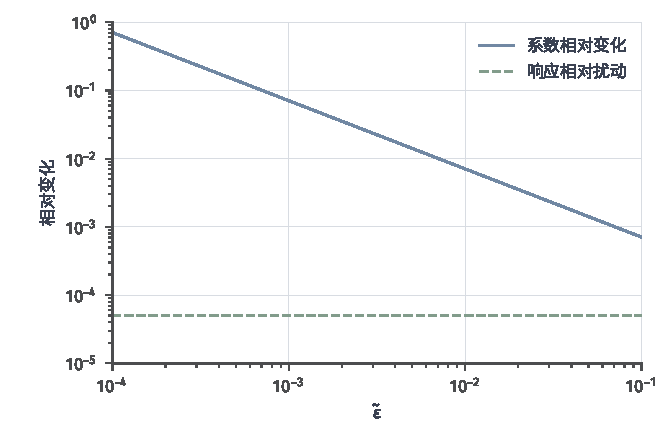
\includegraphics[width=0.92\linewidth]{figures/01-mathematical-preliminaries-upper/02-linear-spaces/matplotlib/matrix-analysis-coefficient-sensitivity/figure.pdf}
 \caption{共线设计的系数分裂：固定右端扰动 $\eta$，$\varepsilon$ 越小，两个系数
 沿相反方向偏离 $(2,0)$ 越远，绝对误差随 $1/\varepsilon$ 增长。}
 \label{fig:matrix-analysis-coefficient-sensitivity}
\end{figure}

\paragraph{拟合值和残差的变化}

系数矩阵固定时，拟合值增量
$\Delta(\bm P_{\operatorname{range}\bm A}\bm b)
=\bm P_{\operatorname{range}\bm A}\Delta\bm b$，投影不放大长度，
$\lVert\Delta\text{拟合}\rVert\leq\lVert\Delta\bm b\rVert$；残差增量落在
$(\operatorname{range}\bm A)^\perp$ 内。对新观测 $\bm a$ 的预测误差为
$\bm a^\top\Delta\hat{\bm x}$，仍受弱方向支配。

\paragraph{固定秩下的伪逆扰动}

$\bm A,\bm B=\bm A+\bm E$ 同为秩 $r$，正奇异值都不小于 $s_0>0$。有限差分恒等式
\[
 \bm B^\dagger-\bm A^\dagger
 =-\bm B^\dagger\bm E\bm A^\dagger
 +\bm B^\dagger(\bm I-\bm A\bm A^\dagger)
 -(\bm I-\bm B^\dagger\bm B)\bm A^\dagger
\]
由 Penrose 条件（\ref{thm:matrix-analysis-pseudoinverse-minimum-norm}）直接
验证；三项分别是主项与补空间耦合。在分离条件下，
\begin{equation}
 \lVert\bm B^\dagger-\bm A^\dagger\rVert
 \leq\frac{3\lVert\bm E\rVert}{s_0^2}.
 \label{eq:ch06-pseudoinverse-fixed-rank-perturbation}
\end{equation}
非主项的界来自 $\ker\bm B$ 与 $(\operatorname{range}\bm A)^\perp$ 的夹角：
对 $\bm u\in(\operatorname{range}\bm A)^\perp$，
$\lVert\bm P_{\ker\bm B}\bm u\rVert=\lVert\bm E\bm u\rVert/s_0$。

\paragraph{正奇异值的分离条件}

$\lVert\bm E\rVert<\sigma_r(\bm A)$ 只排除原方向被完全破坏，不足以保证秩不变：
零方向可能被扰动抬出一个任意小的正奇异值。式~\eqref{eq:ch06-pseudoinverse-fixed-rank-perturbation}
要求双方正奇异值都被 $s_0$ 压住，谱值分离由\ref{sec:ls-spectral-value-sensitivity}的
Weyl 界保证。

\paragraph{秩变化处的不连续性}

$\bm A=\operatorname{diag}(1,0)$，$\bm B_\varepsilon=\operatorname{diag}(1,\varepsilon)$
秩均改变：$\bm A^\dagger=\operatorname{diag}(1,0)$，而
$\bm B_\varepsilon^\dagger=\operatorname{diag}(1,1/\varepsilon)$，
$\varepsilon\to0$ 时不收敛到 $\bm A^\dagger$。秩边界上伪逆无连续界。

\subsubsection{正则化估计}
\label{sec:ls-regularized-estimate-sensitivity}

\paragraph{不稳定方向与正则化过滤}

普通伪逆按 $1/\sigma_i$ 放大噪声；截断SVD保留 $\sigma_i>\tau$ 的方向，
岭回归把增益压成滤波器 $\sigma_i/(\sigma_i^2+\lambda)$
（\ref{eq:matrix-analysis-ridge-filter-factor}，定义与目标在\ref{sec:ls-regularized-ls}）。
二者都主动削弱小奇异方向，代价是损失对应信号。

\paragraph{截断阈值的变化与跳变}

截断阈值 $\tau$ 穿过某个奇异值时，算子突然增删一个方向，估计量发生跳变；
阈值不是连续参数，选择要对照噪声水平而非拟合误差。

\paragraph{岭估计的连续收缩}

$\sigma_i^2+\lambda\geq2\sigma_i\sqrt\lambda$，故岭增益
$\sigma_i/(\sigma_i^2+\lambda)\leq1/(2\sqrt\lambda)$，增益有上界、连续变化；
拟合收缩因子 $\sigma_i^2/(\sigma_i^2+\lambda)<1$ 同时压低信号，这是偏差来源。

\paragraph{偏差和噪声放大的分解}

把 $\bm x_\lambda$ 沿SVD方向写成信号部分与噪声部分：信号被
$\sigma_i^2/(\sigma_i^2+\lambda)$ 收缩形成\term{偏差}（bias），噪声被
$\sigma_i/(\sigma_i^2+\lambda)$ 放大形成噪声项；$\lambda$ 增大两者此消彼长。
零奇异方向在普通伪逆与岭估计中都给出零，不恢复任何信息。

\paragraph{参数尺度与保留信息}

$\lambda$ 与 $\tau$ 的数值依赖特征单位：重新缩放某列后，同样的滤波强度对应
不同方向。比较不同设计的参数值没有意义，保留的信号比例才是共同口径。

\paragraph{一般惩罚算子的扰动}

一般 $\bm L$（差分惩罚等）与 $\bm A$ 不共享奇异方向，不能照搬SVD滤波器；
目标化为增广系统 $\begin{bmatrix}\bm A\\ \sqrt\lambda\,\bm L\end{bmatrix}$ 的
最小二乘，正规方程为 $(\bm A^\top\bm A+\lambda\bm L^\top\bm L)\bm x=\bm A^\top\bm y$，
公共零空间 $\ker\bm A\cap\ker\bm L$ 条件（\ref{eq:linear-algebra-tikhonov-common-nullspace}）
决定唯一性，扰动不改变该空间时解的结构稳定。可算例：$\bm A=\bm I_2$、
$\bm L=[1\ -1]$、$\bm y=(1,0)^\top$、$\lambda=1/2$，正规方程解得
$\bm x_\lambda=(3/4,1/4)^\top$——平均水平 $(x_1+x_2)/2=1/2$ 保持，相邻差由 $1$
缩为 $1/2$；而 $\bm L=\bm I$ 的岭回归给出 $(2/3,0)^\top$，不保持原平均水平，
说明一般 $\bm L$ 压缩的是自己指定的方向，不能逐方向套用岭滤波器。

\paragraph{噪声尺度误差与参数敏感度}

差异原则（\ref{eq:ls-discrepancy-constrained}）按噪声尺度 $\delta$ 选 $\lambda$：
$R(\lambda)$ 单调不增、$P(\lambda)$ 单调不减（\ref{sec:ls-method-selection}），
$\delta$ 的估计误差直接转化为 $\lambda$ 偏差；$\delta$ 低于最小可达残差时约束
恒松弛，$\delta$ 过大则退回普通最小二乘。本节只写参数对噪声尺度的敏感度，
不复述差异原则的定义与二分算法。

\subsection{谱值与子空间的敏感度}
\label{sec:ls-spectral-sensitivity}
\label{sec:linear-algebra-spectral-stability}
\label{sec:ch06-spectral-stability}

\subsubsection{谱值}
\label{sec:ls-spectral-value-sensitivity}

\paragraph{实对称特征值的有序比较}

实对称矩阵（\ref{thm:ls-real-symmetric-spectral}）的特征值全为实数，按降序排列
$\lambda_1\geq\cdots\geq\lambda_d$；扰动后 $\widetilde\lambda_1\geq\cdots\geq\widetilde\lambda_d$，
按同一次序逐个比较，不允许重新配对。

\paragraph{极值刻画与Weyl界}

Courant--Fischer 极值刻画由 Rayleigh 商（\ref{def:matrix-analysis-rayleigh-quotient}）
在子空间约束上取极小极大给出。取 $\bm A$ 的前 $k$ 维顶部子空间，$\bm E$ 在任意单位向量上的二次型
不超过 $\lVert\bm E\rVert_2$，故 $\widetilde\lambda_k\geq\lambda_k-\lVert\bm E\rVert_2$；
对称地用底部子空间得 $\widetilde\lambda_k\leq\lambda_k+\lVert\bm E\rVert_2$。

\begin{theorem}[Weyl特征值扰动界]
\label{thm:ls-weyl-eigenvalue}
对实对称 $\bm A,\bm E\in\mathbb R^{d\times d}$，按降序配对的特征值满足
\begin{equation}
 |\widetilde\lambda_k-\lambda_k|
 \leq\lVert\bm E\rVert_2,
 \qquad k=1,\dots,d.
 \label{eq:matrix-analysis-weyl-eigenvalue-perturbation}
\end{equation}
\end{theorem}

\begin{proof}
$\bm A+\bm E$ 的第 $k$ 大特征值是 $k$ 维子空间上 Rayleigh 商的极小极大。在
$\bm A$ 前 $k$ 个特征向量张成的子空间内，
$\bm x^\top(\bm A+\bm E)\bm x\geq\lambda_k\lVert\bm x\rVert^2-\lVert\bm E\rVert_2\lVert\bm x\rVert^2$，
给出下界；$\bm A$ 后 $d-k+1$ 维子空间给出上界。两式合起来即
~\eqref{eq:matrix-analysis-weyl-eigenvalue-perturbation}。
\end{proof}
该界不需要谱隙，孤立与重合的特征值都适用。

\paragraph{奇异值的绝对扰动界}

把 $\bm A\in\mathbb R^{m\times n}$ 嵌入对称分块矩阵
$\mathcal H(\bm A)=\begin{smallmatrix}\bm0&\bm A\\\bm A^\top&\bm0\end{smallmatrix}$，
其特征值为 $\pm\sigma_i$（\ref{thm:ls-svd-existence}）。$\mathcal H(\bm E)$ 的
谱范数等于 $\lVert\bm E\rVert_2$，对 $\mathcal H(\bm A)$ 与 $\mathcal H(\bm E)$
用 Weyl 界，得
\begin{equation}
 |\widetilde\sigma_i-\sigma_i|\leq\lVert\bm E\rVert_2.
 \label{eq:matrix-analysis-singular-value-perturbation}
\end{equation}
谱值读数本身稳定，不需要谱隙。

\paragraph{实可对角化矩阵的特征坐标}

实可对角化条件（\ref{sec:ls-matrix-powers}）下
$\bm A=\bm V\Lambda\bm V^{-1}$，
$\mu$ 是 $\bm A+\bm E$ 的特征值、$\bm w$ 为对应特征向量。由
$(\bm A+\bm E)\bm w=\mu\bm w$，左乘 $\bm V^{-1}$ 并整理，
\[
 (\Lambda-\mu\bm I)\bm V^{-1}\bm w
 =-\bm V^{-1}\bm E\bm w.
\]

\paragraph{特征基条件数与Bauer--Fike型界}

取离 $\mu$ 最近的 $\lambda_k$，左侧除以 $|\mu-\lambda_k|$，取范数得
\[
 |\mu-\lambda_k|
 \leq\lVert\bm V\rVert_2\lVert\bm V^{-1}\rVert_2\lVert\bm E\rVert_2
 =\kappa_2(\bm V)\lVert\bm E\rVert_2.
\]
特征向量基越病态（$\kappa_2(\bm V)$ 越大），特征值扰动界越宽；这与对称情形
$\bm V$ 正交、$\kappa_2(\bm V)=1$ 形成对照。

\paragraph{非正规性与实谱范围的限制}

非正规矩阵不能照搬对称 Weyl 界。例子 $\bm A=\begin{smallmatrix}0&1\\0&0\end{smallmatrix}$
幂零，特征值全为 $0$；左下角加 $\varepsilon$ 后
$\bm A+\bm E=\begin{smallmatrix}0&1\\\varepsilon&0\end{smallmatrix}$，
特征值为 $\pm\sqrt\varepsilon$，扰动是 $O(\sqrt\varepsilon)$ 而非 $O(\varepsilon)$；
$\varepsilon<0$ 时根本没有实特征值。非正规性使实谱对小扰动的响应失去线性
尺度。

\subsubsection{子空间}
\label{sec:ls-subspace-sensitivity}

\paragraph{基的旋转与子空间不变}

同一子空间的基可以旋转、取负号，单个基向量的变化不能直接当作子空间误差；
重特征值对应的整簇方向内部怎么转都不改变子空间。比较对象必须是子空间本身，
而不是某一组基向量。

\paragraph{主夹角的几何定义}

两个子空间的几何距离由主夹角度量，它对基的旋转与取负号都不变。

\begin{definition}[主夹角]
\label{def:matrix-analysis-principal-angles}
设 $\bm Q,\widetilde{\bm Q}\in\mathbb R^{d\times r}$ 列规范正交，分别张成 $r$ 维
子空间。交叉Gram矩阵 $\bm Q^\top\widetilde{\bm Q}$ 的奇异值为
$\cos\theta_1,\dots,\cos\theta_r$，其中 $0\leq\theta_1\leq\cdots\leq\theta_r\leq\pi/2$，
这些 $\theta_i$ 是两个子空间的\term{主夹角}（principal angles）。
\end{definition}

\paragraph{交叉Gram矩阵与主夹角计算}

对 $\bm Q^\top\widetilde{\bm Q}$ 作SVD，奇异值即 $\cos\theta_i$，配对的主方向
$\bm a_i$（取自 $\operatorname{range}\bm Q$）与 $\bm b_i$（取自
$\operatorname{range}\widetilde{\bm Q}$）满足
$\bm b_i=\cos\theta_i\,\bm a_i+\sin\theta_i\,\bm c_i$，
$\bm c_i\perp\bm a_i$。基换为 $\bm Q\bm R$、$\widetilde{\bm Q}\widetilde{\bm R}$
（$\bm R$ 正交）后，交叉矩阵右乘正交因子，奇异值不变，故主夹角与基的选择无关。

\paragraph{投影差与基无关的误差}

正交投影 $\bm P=\bm Q\bm Q^\top$、$\widetilde{\bm P}=\widetilde{\bm Q}\widetilde{\bm Q}^\top$。
用主夹角把 $2\times2$ 块写成 $\begin{smallmatrix}\cos\theta&\sin\theta\\-\sin\theta&\cos\theta\end{smallmatrix}$，
直接计算得
\[
 \lVert\bm P-\widetilde{\bm P}\rVert_2=\sin\theta_r,
 \qquad
 \frac12\lVert\bm P-\widetilde{\bm P}\rVert_{\mathrm F}^2
 =\sum_{i=1}^r\sin^2\theta_i.
\]
投影差是基无关的子空间误差度量。

\paragraph{谱隙、残差与子空间变化}

孤立特征方向的 Davis--Kahan 型界：$\bm A$ 对称，$\lambda_k$ 与其余谱的分离量为
$\gamma=\min_{j\neq k}|\lambda_j-\lambda_k|$，$\bm q$ 是单位近似特征方向，
残差 $\rho=\lVert\bm A\bm q-\mu\bm q\rVert$，则
\begin{equation}
 \sin\angle(\bm q,\bm q_k)
 \leq\frac{\lVert\bm E\rVert_2+\rho}{\gamma}.
 \label{eq:matrix-analysis-eigenvector-gap-bound}
\end{equation}
分离量 $\gamma$ 出现在分母：谱隙越小，方向对扰动越敏感。二维例子
$\bm A_\alpha=\operatorname{diag}(\alpha,-\alpha)$（两特征值相距 $2\alpha$），
$\bm E_\varepsilon=\varepsilon\begin{smallmatrix}0&1\\1&0\end{smallmatrix}$，
扰动后最大特征方向转过
$\theta=\tfrac12\arctan(\varepsilon/\alpha)\approx\varepsilon/(2\alpha)$，
图~\ref{fig:matrix-analysis-gap-direction}给出几何。整簇比较时，分离量取目标簇
与簇外最近谱值的单边距离，簇内特征值不需要彼此分开。

\begin{figure}
 \centering
 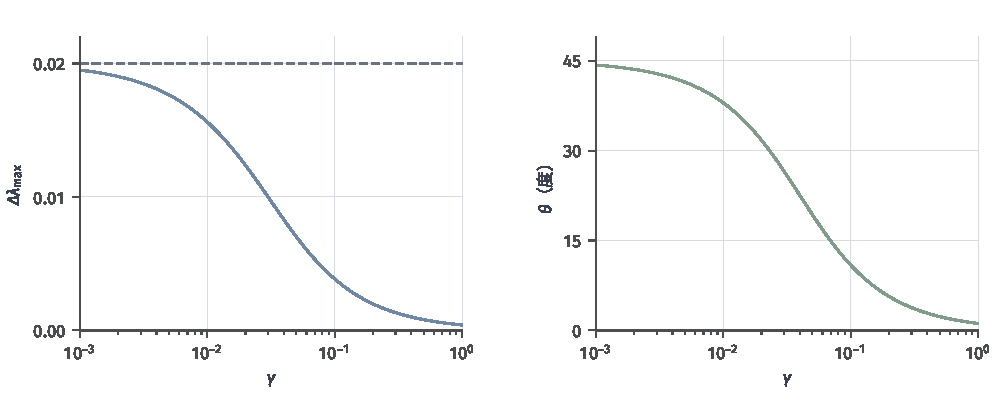
\includegraphics[width=0.92\linewidth]{figures/01-mathematical-preliminaries-upper/02-linear-spaces/matplotlib/matrix-analysis-gap-direction/figure.pdf}
 \caption{谱隙方向示意：$\bm A_\alpha$ 的两个特征值相距 $2\alpha$（谱隙），
 交叉扰动 $\varepsilon$ 把最大特征方向转过约 $\varepsilon/(2\alpha)$；
 谱隙越小，同样扰动转过的角度越大。}
 \label{fig:matrix-analysis-gap-direction}
\end{figure}

\paragraph{重特征值的整簇比较}

$\bm A=\operatorname{diag}(2,2,0)$ 中重特征值 $2$ 的平面内任意单位向量都是
特征方向，单独比较某个向量没有意义；应比较整个二维子空间。$\lambda\bm I$ 的
特征空间全空间，任何方向都不可区分，单方向误差天然无穷。

\paragraph{左右奇异子空间与Wedin型界}

对秩 $r$ 的 $\bm A$ 与 $\bm B=\bm A+\bm E$，记左、右目标子空间投影，残差为
$\lVert(\bm I-\widetilde{\bm U}\widetilde{\bm U}^\top)\bm A\rVert$ 与
$\lVert\bm A(\bm I-\widetilde{\bm V}\widetilde{\bm V}^\top)\rVert$。Wedin 型界把残差、
谱隙与子空间夹角连起来：
\begin{equation}
 \sin\theta\leq\frac{\sqrt{2r}\,\lVert\bm E\rVert_2}{\operatorname{sep}_{\mathrm W}},
 \label{eq:matrix-analysis-singular-subspace-gap}
\end{equation}
$\operatorname{sep}_{\mathrm W}$ 是目标奇异值与簇外最近奇异值的分离量；
$\sqrt{2r}$ 是粗化常数，精确块矩阵论证见\scite{math-golub2013matrix}。

\subsubsection{结构逼近}
\label{sec:ls-structured-approximation-sensitivity}

\paragraph{低秩重构与主方向的不同输出}

最佳秩 $k$ 逼近的误差由 $\sigma_{k+1}$ 控制（\ref{thm:ls-best-low-rank}），
谱值读数稳定；但逼近用到的主方向是否稳定，要看截断处是否存在谱隙，二者不是
同一个输出。

\paragraph{谱值误差与方向误差的组合}

截断SVD $\bm A_k$ 的矩阵误差同时包含谱值误差（Weyl 界）与子空间误差
（Davis--Kahan/Wedin 界）：谱值项逐项被 $\lVert\bm E\rVert$ 控制，方向项除以
分离量，后者在谱隙消失时主导。

\paragraph{截断边界和谱簇选择}

截断线穿过重复或成簇的奇异值时，边界方向对扰动敏感；此时报告整簇张成的子空间，
不单独宣称某一个主方向。选择簇边界的依据是谱值间距与噪声水平，不是拟合误差
单独决定。

\paragraph{非唯一逼近的连续性边界}

谱范数意义下最佳秩 $k$ 逼近在奇异值重复时可不唯一；Frobenius 口径由SVD唯一达到。
接近重复奇异值时，解的选择随扰动跳变，连续性只在选定口径与唯一区讨论。

\paragraph{正交逼近中的秩与选解}

极分解规范因子 $\bm Q=\bm U\bm V^\top$（\ref{def:matrix-analysis-polar-decomposition}）
在秩亏处的正交延拓不唯一；与\ref{sec:ls-ordinary-ls-sensitivity}的伪逆同理，
延拓边界上不追求连续单方向。

\subsection{矩阵函数的敏感度}
\label{sec:ls-matrix-function-sensitivity}
\label{sec:linear-algebra-matrix-function-stability}
\label{sec:ch06-matrix-function-stability}

\subsubsection{幂与指数}
\label{sec:ls-powers-exponential-sensitivity}

\paragraph{有限幂差的望远镜展开}

$(\bm A+\bm E)^k-\bm A^k$ 按乘积位置逐次插入 $\bm E$，精确展开为
\[
 (\bm A+\bm E)^k-\bm A^k
 =\sum_{j=0}^{k-1}(\bm A+\bm E)^{k-1-j}\bm E\bm A^j.
\]
每一项在固定位置插入一个 $\bm E$，这是有限增量的恒等式。

\paragraph{扰动插入位置与非交换乘法}

$k=2$ 时 $(\bm A+\bm E)^2-\bm A^2=\bm A\bm E+\bm E\bm A+\bm E^2$；
$\bm A\bm E$ 与 $\bm E\bm A$ 一般不相等，插入左侧与右侧不能合并，这是非交换性
带来的额外项，标量情形才退化为 $2\bm A\bm E$。

\paragraph{各位置传播与范数界}

取 $M=\max\{\lVert\bm A\rVert,\lVert\bm A+\bm E\rVert\}$，每一项范数不超过
$M^{k-1}\lVert\bm E\rVert$，共 $k$ 项，故
\[
 \lVert(\bm A+\bm E)^k-\bm A^k\rVert
 \leq kM^{k-1}\lVert\bm E\rVert.
\]
界随固定阶数 $k$ 线性增长，$k$ 本身进入常数。

\paragraph{矩阵指数的逐幂增量}

$\bm e^{\bm A}=\sum_{k=0}^\infty\bm A^k/k!$（\ref{sec:ls-matrix-exponential}），
把 $(\bm A+\bm E)^k$ 的望远镜展开逐项代入，指数差由各阶幂差贡献。

\paragraph{绝对级数控制与有限增量界}

不使用积分公式，直接用绝对级数控制：$\lVert e^{\bm B}\rVert\leq e^{\lVert\bm B\rVert}$，
结合幂差界逐项求和，得到随 $\lVert\bm A\rVert$、$\lVert\bm E\rVert$ 增长的粗界。
它只保证局部连续性，不是紧估计。

\paragraph{固定参数与长期变化的区别}

本节估计固定 $k$ 或固定参数处的一次函数响应；$\bm A^k$ 随 $k$ 增长或衰减的长期
行为是收敛分析的对象（\ref{sec:ls-convergence}）。$2\bm I$ 与 $\bm I/2$ 条件数
同为 $1$，幂却分别增长与衰减，条件数不回答长期问题。

学完多元微积分后可回读以下一阶响应材料，它不作为本节主线前提，有限增量论证已
独立成立。矩阵函数的一阶响应由 Fréchet 导数给出
\begin{equation}
 \mathrm d f_{\bm A}(\bm E)
 =\lim_{t\to0}\frac{f(\bm A+t\bm E)-f(\bm A)}{t},
 \label{eq:matrix-analysis-frechet-derivative}
\end{equation}
可对角化时它由除差函数
\begin{equation}
 f^{[1]}(\lambda_i,\lambda_j)
 =\frac{f(\lambda_i)-f(\lambda_j)}{\lambda_i-\lambda_j}
 \label{eq:matrix-analysis-frechet-divided-difference}
\end{equation}
经 $\bm V,\bm V^{-1}$ 作用得到；矩阵指数的 Fréchet 导数可写成积分
\begin{equation}
 \mathrm d\exp_{\bm A}(\bm E)
 =\int_0^1 e^{s\bm A}\bm E\,e^{(1-s)\bm A}\,\mathrm ds.
 \label{eq:matrix-analysis-exponential-frechet-derivative}
\end{equation}

\subsubsection{平方根与对数}
\label{sec:ls-square-root-log-sensitivity}

\paragraph{同一分支上的平方根差}

$\bm A\succ0$，正定平方根 $\bm S\succ0$ 满足 $\bm S^2=\bm A$；$\bm B=\bm A+\bm E$
仍正定，取同一正分支 $\widehat{\bm S}\succ0$，$\widehat{\bm S}^2=\bm B$。另一分支
$-\bm S$ 残差同为零，必须先选定正分支。

\paragraph{Sylvester差方程的推导}

记 $\bm D=\widehat{\bm S}-\bm S$，由
$\widehat{\bm S}^2-\bm S^2=\widehat{\bm S}\bm D+\bm D\bm S=\bm E$，
这正是以 $\widehat{\bm S},\bm S$ 为系数的Sylvester方程（\ref{def:matrix-analysis-sylvester-equation}）；
一阶近似为 $\bm S\bm Z+\bm Z\bm S=\bm E$。不能写成 $2\bm S\bm Z=\bm E$，
因为 $\bm S$ 与 $\bm Z$ 一般不交换。

\paragraph{最小特征值与平方根响应}

$\bm S$ 的本征基下，$(s_i+s_j)Z_{i,j}=E_{i,j}$，故
$\lVert\bm Z\rVert_{\mathrm F}\leq\lVert\bm E\rVert_{\mathrm F}/(2s_{\min})$，
$s_{\min}=\sqrt{\lambda_{\min}(\bm A)}$。例子 $\bm S=\operatorname{diag}(1,2)$，
$\bm E$ 的非对角元 $e$ 给出 $Z_{1,2}=e/(1+2)=e/3$，而不是 $e/2$。

\paragraph{正定对数的定义域保持}

$\log\bm A$ 只对正定矩阵定义（\ref{sec:ls-matrix-functions}）；扰动保持正定的
余量由 $\lambda_{\min}(\bm A)$ 决定，边界处先失去定义域，再谈对数误差。

\paragraph{接近零谱方向的对数放大}

对数沿 $\lambda$ 方向的响应为 $1/\lambda$，$\lambda_{\min}\to0$ 时无界；半正定
边界上对数不连续，与平方根的有界响应形成对照。

\paragraph{函数残差与分支核验}

记 $\bm R=\widehat{\bm S}^2-\bm A$，精确差方程
$\widehat{\bm S}\bm D+\bm D\bm S=\bm R$，故
$\lVert\bm D\rVert_{\mathrm F}
\leq\lVert\bm R\rVert_{\mathrm F}/(\lambda_{\min}(\widehat{\bm S})+\sqrt{\lambda_{\min}(\bm A)})$。
核验分支：残差小不区分 $\pm\bm S$，需另查正定性；$\log\det\bm A$ 是标量行列式
读数，与矩阵对数 $\log\bm A$ 不是同一对象。

\subsection{数值算法的稳定性}
\label{sec:ls-numerical-stability}

\subsubsection{数据误差与计算误差}
\label{sec:ls-data-computation-error}
\label{sec:linear-algebra-error-propagation}
\label{sec:ch06-error-propagation}

\paragraph{数据误差与计算误差的分解}

实际计算结果 $\widehat{\bm y}$ 与理想答案的差拆成两段：
\[
 \widehat{\bm y}-F(\bm z)
 =\underbrace{[\widehat{\bm y}-F(\bm z+\Delta\bm z)]}_{\text{算法计算误差}}
 +\underbrace{[F(\bm z+\Delta\bm z)-F(\bm z)]}_{\text{数据扰动误差}}.
\]
前者由算法在机器上的执行产生，后者由输入本身的误差经条件数放大，二者归因不同。

\paragraph{精确解与实际计算结果}

\term{前向误差}（forward error）即 $\widehat{\bm y}-F(\bm z)$，是最终直接测量的
误差；它同时受问题条件与算法质量影响，不能单独归给其中一方。

\paragraph{后向误差的允许集合}

\term{后向误差}（backward error）寻找最小的输入扰动 $\Delta\bm z$，使 $\widehat{\bm y}$
恰好是 $F(\bm z+\Delta\bm z)$ 的精确解。允许集合由任务规定：只允许右端改变，
或同时允许矩阵改变并保持对称；在集合内取范数最小的扰动作为后向误差度量。

\paragraph{舍入误差的局部积累}

机器实数每次运算满足浮点模型
\begin{equation}
 \operatorname{fl}(x\circ y)=(x\circ y)(1+\delta),
 \qquad |\delta|\leq u,
 \label{eq:ch06-floating-point-model}
\end{equation}
双精度 $u=2^{-53}\approx1.1\times10^{-16}$。$n$ 步运算的局部舍入累计常数为
$\gamma_n=nu/(1-nu)$，步骤越多累计越大；抵消与放大还会在中间步引入额外相对误差。

\paragraph{条件数连接后向与前向误差}

前向误差由后向误差经条件数放大：
\[
 \frac{\lVert\widehat{\bm y}-F(\bm z)\rVert}
      {\lVert F(\bm z)\rVert}
 \lesssim\kappa\cdot\frac{\lVert\Delta\bm z\rVert}{\lVert\bm z\rVert}.
\]
后向误差衡量算法把答案安放到了哪个邻近问题上，条件数再决定这个邻近问题拉开多远。

\begin{definition}[后向稳定]
\label{def:matrix-analysis-backward-stability}
算法对所有合法输入给出的结果，都是某个邻近输入的精确解，且后向误差以机器精度
$u$ 乘以与规模无关的常数为界，则称算法\term{后向稳定}（backward stable）。
\end{definition}

\paragraph{稳定算法与病态问题的区别}

后向稳定只保证 $\widehat{\bm y}$ 是邻近问题的精确解，不保证 $\widehat{\bm y}$
接近 $F(\bm z)$：病态问题（$\kappa$ 大）中，很小的后向误差经放大仍得到远离理想
答案的前向误差。稳定算法不能治愈问题本身的病态。

\subsubsection{分解与求解}
\label{sec:ls-factorization-solve}

\paragraph{计算因子与邻近矩阵}

向后误差分析把实际分解写成邻近矩阵的精确分解：算出的 $\widehat{\bm L},\widehat{\bm U}$
满足 $\widehat{\bm L}\widehat{\bm U}=\bm A+\Delta\bm A$，$\lVert\Delta\bm A\rVert$
以 $cu\lVert\bm A\rVert$ 为界，$c$ 是规模温和的误差常数。

\paragraph{消元主元增长与误差常数}

Gaussian 消元的误差常数含主元增长因子；部分选主元把增长控制在实用范围，但不
改变问题条件数。增长因子是算法实现的局部量，与 $\kappa(\bm A)$ 分别估计。

\paragraph{Cholesky的正定结构边界}

Cholesky 成功分解要求矩阵正定（\ref{sec:ls-direct-methods}）；接近半正定时代数
上仍正定但数值上可能失败，失败本身不区分“真的奇异”与“余量不足”。加对角常数
改变的是任务，不能当作修复。

\paragraph{QR和SVD的误差解释}

Householder QR 的计算因子后向正交，后向误差以 $cu$ 为界；经典Gram--Schmidt 会
逐步丢失正交性，后向界更宽。SVD 直接在 $\bm A$ 上工作，避免形成 Gram 矩阵，
子空间与伪逆由分解直接读出。

\paragraph{正规方程的条件数平方效应}

形成 $\bm A^\top\bm A$ 把条件数平方：
\begin{equation}
 \kappa_2(\bm A^\top\bm A)=\kappa_2(\bm A)^2.
 \label{eq:matrix-analysis-normal-equation-condition-square}
\end{equation}
共线例子 $\bm X_\varepsilon=
\left[\begin{smallmatrix}1&1\\0&\varepsilon\end{smallmatrix}\right]$
（见\ref{sec:ls-ordinary-ls-sensitivity}），$\kappa_2(\bm X_\varepsilon)\approx2/\varepsilon$，
而 $\bm X_\varepsilon^\top\bm X_\varepsilon=
\left[\begin{smallmatrix}1&1\\1&1+\varepsilon^2\end{smallmatrix}\right]$
的小特征值约为 $\varepsilon^2$，正规方程条件数约 $4/\varepsilon^2$；
$\varepsilon^2$ 尺度的方向在浮点中直接与零不可区分，信息先于求解损失。

\paragraph{问题病态与实现稳定性的分工}

表~\ref{tab:matrix-analysis-solver-conditions}把各路径的主要误差来源与条件数
角色并列；迭代法的残差与误差区别、收敛速率属\ref{sec:ls-convergence}，此处只
记录稳定性分工。

\begin{table}
\centering
\small
\setlength{\tabcolsep}{5pt}
\caption{直接法与迭代法的稳定性分工：条件数放大问题本身的误差，实现常数控制算法
局部误差，二者不可互相替代。}
\label{tab:matrix-analysis-solver-conditions}
\begin{tabular}{llll}
方法 & 主要误差来源 & 条件数角色 & 可靠输出 \\
\hline
带主元LU & 主元增长、回代 & 放大解误差 & 良态一般矩阵 \\
QR & 正交变换后向误差 & 不平方 & 近共线最小二乘 \\
Cholesky & 正定余量 & 放大解误差 & 正定且余量充足 \\
SVD与伪逆 & 分解本身 & 给出子空间 & 秩未知、需要选解 \\
共轭梯度 & 能量范数残差 & 决定迭代步数 & 正定对称（收敛见\ref{sec:ls-convergence}） \\
GMRES & 残差最小化 & 决定迭代步数 & 一般非对称（收敛见\ref{sec:ls-convergence}） \\
\end{tabular}
\end{table}

\subsubsection{结果核验}
\label{sec:ls-result-verification}
\label{sec:matrix-analysis-error-verification}

\paragraph{原系统残差与邻近问题}

对候选解 $\widehat{\bm x}$，原系统残差
\begin{equation}
 \bm r=\bm b-\bm A\widehat{\bm x}
 \label{eq:matrix-analysis-residual}
\end{equation}
直接可算；由 $\bm A\bm x=\bm b$ 得 $\bm x-\widehat{\bm x}=\bm A^{-1}\bm r$，
残差经逆范数变成解误差。

\paragraph{小残差不等于小解误差}

相对解误差满足
\[
 \frac{\lVert\widehat{\bm x}-\bm x\rVert}{\lVert\bm x\rVert}
 \leq\kappa(\bm A)\frac{\lVert\bm r\rVert}{\lVert\bm b\rVert}.
\]
$\bm A=\operatorname{diag}(1,\varepsilon)$，$\bm b=(1,\varepsilon)^\top$，
候选 $\widehat{\bm x}=(1,0)^\top$：精确解为 $(1,1)^\top$，残差 $\bm r=(0,\varepsilon)^\top$，
绝对残差范数为 $\varepsilon$，相对残差 $\lVert\bm r\rVert/\lVert\bm b\rVert
=\varepsilon/\sqrt{1+\varepsilon^2}\to0$，而相对解误差趋于 $1/\sqrt2$。
病态时残差小不保证解准。

\paragraph{联合扰动的归一化后向误差}

允许矩阵与右端同时改变，归一化后向误差定义为
\begin{equation}
 \eta_2(\widehat{\bm x})
 =\frac{\lVert\bm r\rVert_2}
       {\lVert\bm A\rVert_2\lVert\widehat{\bm x}\rVert_2+\lVert\bm b\rVert_2}
 \label{def:matrix-analysis-normwise-backward-error}
\end{equation}
令 $d_0=\lVert\bm A\rVert_2\lVert\widehat{\bm x}\rVert_2+\lVert\bm b\rVert_2$，
$\widehat{\bm x}\neq\bm0$ 时可取
\[
 \Delta\bm A=\frac{\lVert\bm A\rVert_2}{d_0}\,
 \frac{\bm r\,\widehat{\bm x}^\top}{\lVert\widehat{\bm x}\rVert_2},
 \qquad
 \Delta\bm b=-\frac{\lVert\bm b\rVert_2}{d_0}\,\bm r,
\]
两项分别按 $\lVert\bm A\rVert_2$、$\lVert\bm b\rVert_2$ 缩放，各自的相对尺度都
恰达到下界 $\eta_2$，且 $(\bm A+\Delta\bm A)\widehat{\bm x}=\bm b+\Delta\bm b$。
代入联合扰动界，当 $\kappa\eta_2<1$ 时解误差不超过
$2\kappa\eta_2/(1-\kappa\eta_2)$。

\paragraph{零尺度下的绝对核验}

$\bm b=\bm0$ 时分母无任意尺度，改用绝对残差；最小二乘另查正规方程残差
$\bm g=\bm A^\top\bm r=\bm0$ 与最小范数条件 $\widehat{\bm x}\perp\ker\bm A$。
例子 $\bm X=[1\ 1]$、$\bm y=2$，候选 $(3,-1)^\top$ 残差为零但非最小范数，
只有 $\bm g=0$ 与投影核验同时通过才算合格。

\paragraph{递推残差与真实残差}

迭代中递推累加的残差在几步后丢失精度，应以高精度重算 $\bm b-\bm A\widehat{\bm x}$；
递推残差用于递推，真实残差用于停止判断。

\paragraph{迭代改进与停止依据}

用同一分解解 $\bm A\bm d=\bm r_c$ 修正 $\widehat{\bm x}\leftarrow\widehat{\bm x}+\bm d$，
改进幅度受 $\kappa$ 与残差精度双重限制，数据误差到达地板后停止。停止同时核验：
真实残差、归一化后向误差与条件数估计，不以递推残差单独为准。


\section{收敛分析}
\label{sec:ls-convergence}
\label{sec:linear-algebra-convergence-approximation}

~\ref{sec:ls-perturbation}节回答输入小变时输出变多少，本节回答另一个独立问题：
迭代、反复作用和无穷级数在步数趋于无穷时走向哪里、以多快的速度接近、
什么条件下根本不收敛。求解与逼近各章已经给出各方法的更新格式、可执行条件和
核验量，这里不重复教程，只证明误差与残差序列的极限行为：先建立有限维序列本身的
收敛判据，再分别研究固定矩阵的幂、矩阵级数与指数演化、定常迭代、Krylov迭代、
最小二乘迭代、谱方向迭代和矩阵函数迭代，最后把每步新增扰动纳入长期传播并讨论
停止精度。所有结论都在实数、有限维范围内展开；速度估计依赖具体范数和谱分布，
定性收敛与定量速度必须分开报告。

\subsection{有限维序列的收敛}
\label{sec:ls-finite-dimensional-sequences}
\label{sec:linear-algebra-sequence-convergence}

\subsubsection{收敛与误差尺度}

\paragraph{逐坐标误差与范数误差}

固定一组基$(\bm b_1,\ldots,\bm b_d)$，把向量序列$\bm x^{(t)}$写成坐标序列
$x_1^{(t)},\ldots,x_d^{(t)}$。最直接的观察方式是逐坐标比较：第$j$个坐标的误差
为$|x_j^{(t)}-x_j|$，全部坐标都随$t$趋零，等价于坐标最大范数
$\lVert\bm x^{(t)}-\bm x\rVert_c=\max_j|x_j^{(t)}-x_j|$趋零。另一种观察方式是
直接在选定范数$\lVert\cdot\rVert$下比较$\lVert\bm x^{(t)}-\bm x\rVert$。
两种方式描述的是同一个序列，但读数尺度不同：一个坐标偏差很大而其余坐标相消时，
逐坐标读数和欧氏长度可能给出不同的瞬时大小，需要先弄清二者何时互相推出。
复算小例：$\bm x^{(t)}=(1/t,\,-1/t)^{\top}$，逐坐标误差为$1/t$，欧氏长度为
$\sqrt2/t$，两者都趋零但瞬时数值相差$\sqrt2$倍；若换成斜基$\bm b_1=(1,0)$、
$\bm b_2=(1,1)$，同一向量的坐标读数又会改变，因此不能把某一种读数的大小
当作收敛速度本身。

\paragraph{两种收敛描述的等价}

~\ref{thm:ls-norm-equivalence}已经证明有限维任意两范数等价，即存在常数
$c,C>0$使$c\lVert\bm z\rVert_c\leq\lVert\bm z\rVert\leq C\lVert\bm z\rVert_c$。
于是$\lVert\bm x^{(t)}-\bm x\rVert\to0$当且仅当
$\lVert\bm x^{(t)}-\bm x\rVert_c\to0$，而后者又当且仅当每个标量坐标
$x_j^{(t)}\to x_j$。坐标收敛推出范数收敛用右端不等式，反向用左端不等式，
不需要重新证明范数等价本身。必要性方向：若范数趋零而某坐标$j$不趋零，
则$|x_j^{(t)}-x_j|$有正下界，由左端不等式$\lVert\bm x^{(t)}-\bm x\rVert\geq
c|x_j^{(t)}-x_j|$也不能趋零，矛盾。因此“序列是否收敛到某向量”与选择哪个
范数无关，后文可以按论证方便切换欧氏范数、最大范数或任意诱导范数，只在需要
定量界时才指定具体范数。边界：这一等价只在有限维成立；无限维中存在不等价
范数，坐标收敛与范数收敛可以分离，本章不涉及。

\paragraph{误差尺度变换与收敛保持}

等价常数随基和范数改变，但不改变极限本身。作固定可逆坐标变换$\bm z=\bm P\bm x$时，
有限维线性映射在任意范数下有界，故$\bm x^{(t)}\to\bm x$蕴含
$\bm P\bm x^{(t)}\to\bm P\bm x$；逆变换同样有界，反向也成立。证明：由范数等价，
$\lVert\bm P\bm x\rVert\leq C_P\lVert\bm x\rVert$，$\lVert\bm x\rVert\leq
C_{P^{-1}}\lVert\bm P\bm x\rVert$，故$\bm P$与$\bm P^{-1}$都把收敛序列映为
收敛序列。换一组范数、换一组基只重新标度误差，不创造也不消灭极限。这与
~\ref{sec:ls-norms-distances}节的尺度比较一致：定性结论（收敛、有界、闭集
保留极限）只依赖等价类，不依赖常数大小。反例边界：若变换本身随$t$变化
（例如每步换基），上述有界性不再成立，时变坐标下的极限必须单独证明，
不能沿用本段结论。

\paragraph{比较常数与速度表述}

必须把“收敛是否成立”与“以多快收敛”分开。范数等价只给出夹逼常数$c,C$，
它们用于互换存在性结论，不能当作衰减率；同一个极限在不同范数下可能第一步
放大、长期却趋零。定量速度要在具体范数下由递推结构给出，后文各节的几何因子、
谱半径和条件数才承担速度角色，本节只保证“换尺度不改变收敛与否”。例如
$\bm A=\operatorname{diag}(0.5,0.9)$在欧氏范数下每步乘缩，而取一个
非正交相似范数时前几步长度可能上升；存在性结论不变，瞬时放大却属于速度
分析。报告时应先说“是否收敛”，再在指定范数下给出几何因子或步数估计，
不得用等价常数$C$代替衰减率。

\subsubsection{极限的存在}

\paragraph{柯西条件与坐标序列}

极限未知时用柯西条件判别：对任意$\varepsilon>0$，存在$N$使$m,n>N$时
$\lVert\bm x^{(m)}-\bm x^{(n)}\rVert<\varepsilon$。由左端等价不等式，
$|x_j^{(m)}-x_j^{(n)}|\leq c^{-1}\lVert\bm x^{(m)}-\bm x^{(n)}\rVert$，
所以范数柯西列的每个坐标都是实柯西数列。实数的柯西收敛准则保证
每个坐标有实数极限$x_j$，不需要预先知道极限向量。必要性同样成立：若
某坐标不是柯西列，则存在$\varepsilon_0$与无穷多对$m,n$使
$|x_j^{(m)}-x_j^{(n)}|\geq\varepsilon_0$，由等价不等式原序列也不是
柯西列。这一步把向量柯西条件分解为$d$个标量柯西条件，标量完备性是
唯一的实数前提。

\paragraph{实数极限与向量极限的恢复}

把各坐标极限组装成$\bm x=\sum_jx_j\bm b_j$。对$m>N$，
$\lVert\bm x^{(m)}-\bm x\rVert_c=\max_j|x_j^{(m)}-x_j|$，有限个坐标的差同时
趋零，故该最大差趋零，再由右端不等式得到
$\lVert\bm x^{(m)}-\bm x\rVert\to0$。有限性在这里是关键：若坐标个数无穷，
“每个坐标趋零”不能推出最大差趋零（第$j$个坐标在$t=j$后才开始下降），
这正是无限维与有限维的分界。恢复过程只用到有限维数和标量完备性，
不依赖内积或角度。

\paragraph{有限维完备性}

结合上两段：范数柯西列逐坐标取极限、再重组为向量极限并在原范数下收敛，
所以有限维赋范空间在任意范数下都完备。这一结论不依赖欧氏结构，是范数等价的
直接推论；完备性回答“柯西列在本空间内是否有极限”，与线性空间极限的唯一性
（由三角不等式保证：若$\bm x^{(t)}\to\bm x$且$\bm x^{(t)}\to\bm y$，则
$\lVert\bm x-\bm y\rVert\leq\lVert\bm x-\bm x^{(t)}\rVert+
\lVert\bm x^{(t)}-\bm y\rVert\to0$，故$\bm x=\bm y$）是两件事。复算：
$\mathbb R^d$按任何等价范数都完备，因为它与坐标最大范数线性同构且后者
完备；不完备只发生在无限维函数空间。

\paragraph{闭子空间中的极限保留}

~\ref{thm:ls-subspace-closed}证明有限维子空间在任意范数下闭。若序列全部
落在子空间$S$内且$\bm x^{(t)}\to\bm x$，闭性保证$\bm x\in S$，不需要额外
条件。因此闭子空间本身也完备：$S$内的柯西列在全空间取到的极限必然留在$S$内。
证明：把$S$本身看作有限维赋范空间，上段完备性直接适用；全空间中取到的极限
由闭性回到$S$。求解与迭代中常用的特征空间、零空间、值域都是有限维闭子空间，
其极限分量不会逃到子空间外。边界：无限维闭子空间才需要单独证明闭性，
本章全部空间有限，可直接引用。

\paragraph{有界子列与整列收敛的区别}

闭有界集上每个序列都存在收敛子列（~\ref{sec:ls-error-scale-comparison}节的
有限维紧性），但子列存在不等于整列收敛。反例：在$\mathbb R^2$中交替取
$\bm e_1$和$-\bm e_1$，序列有界且两个子列各自常值收敛，整列却在两个点
之间振荡，不趋于任何向量；该序列甚至不是柯西列（相邻两项距离为$2$）。
再如$\bm x^{(t)}=(\sin t,0)^{\top}$，每个子列都可抽出收敛点，但整列在
$[-1,1]$上振荡。因此“抽出一个收敛子列”只能说明有界，证明整列收敛还需
柯西条件或递推给出的逐点压缩（如后文$\lVert\bm e^{(t+1)}\rVert\leq
q\lVert\bm e^{(t)}\rVert$，$q<1$）。

\subsection{矩阵连乘的长期行为}
\label{sec:ls-matrix-power-behavior}
\label{sec:linear-algebra-power-convergence}

\subsubsection{固定矩阵的幂}

\paragraph{重复作用与矩阵幂序列}

对固定方阵$\bm A$反复作用，初值$\bm x^{(0)}$在第$k$步变成
$\bm x^{(k)}=\bm A^k\bm x^{(0)}$。要判断“所有初值是否都衰减”，只检查某一个
初值的轨迹可能恰好没有经过不稳定方向，必须控制整个矩阵幂$\bm A^k$。
动机：单个初值的轨迹由初值在各特征方向上的分量决定，若初值碰巧不含某个
$|\lambda|\geq1$方向，轨迹看起来收敛，换一个初值立即发散。全体初值收敛等价于
$\bm A^k\to\bm0$（矩阵序列在诱导范数下趋零），这比“存在某个收敛初值”强得多。
下面先给全体初值的衰减判据，再处理$\rho(\bm A)=1$边界上的有界、振荡与增长。

\paragraph{次乘性与实幂增长率}

诱导范数次乘性给出$\lVert\bm A^{k+\ell}\rVert\leq\lVert\bm A^k\rVert
\lVert\bm A^\ell\rVert$，特别地$\lVert\bm A^k\rVert\leq\lVert\bm A\rVert^k$。
若$\lVert\bm A\rVert<1$，则$\lVert\bm A^k\rVert\leq\lVert\bm A\rVert^k\to0$，
这是一条可直接核验的充分条件；但它不是必要条件，因为范数可以通过非正交方向的
相消把瞬时长度放大，长期却由谱决定。复算：$\bm A=\operatorname{diag}(0.5,0.9)$
在任意范数下都有$\rho=0.9<1$，但在某个斜置等价范数中$\lVert\bm A\rVert$可
大于$1$，充分条件失效而衰减仍然成立。次乘性也给出有界性：$\lVert\bm A\rVert\leq1$
只保证$\lVert\bm A^k\rVert$不超过$\lVert\bm A\rVert^k\leq1$，不保证趋零；
等号情形（如$\bm A$为正交旋转）长度恒定，需逐类判别。

\paragraph{分块幂估计与几何上界}

由实Schur或实分裂的Jordan分块表示（见下一小节），每个块的幂都是有限次多项式
乘以模长$r^k$。对任意$r>\rho(\bm A)$，多项式增长$k^s$总能被较大的几何因子
$r^k$控制，因为$\lim_{k\to\infty}k^s/r^k=0$，故存在常数$C_r$使
$\lVert\bm A^k\rVert\leq C_r r^k$。证明要点：每个特征值$\lambda_i$满足
$|\lambda_i|<r$，有限个块各自有界，换基矩阵固定，合并即得。这一估计把
“谱半径小于某数”翻译成可用于递推的几何上界，常数$C_r$依赖矩阵和$r$，
随$r\downarrow\rho(\bm A)$可能增大；当$\rho(\bm A)=0$（幂零矩阵）时
$\bm A^s=\bm0$，有限步后恰为零，比几何衰减更快。

\paragraph{谱半径和所有初值的衰减}

\begin{theorem}[固定矩阵幂的衰减判据]
\label{thm:ls-power-decay}
对有限实方阵$\bm A$，$\bm A^k\to\bm0$当且仅当谱半径
$\rho(\bm A)=\max_i|\lambda_i(\bm A)|<1$。
\end{theorem}
\begin{proof}
必要性：若$\bm A^k\to\bm0$，对任一实特征向量$\bm v$与特征值$\lambda$，
$\bm A^k\bm v=\lambda^k\bm v\to\bm0$，故$|\lambda|<1$；非实共轭对在实二维
块中以模$|\lambda|$旋转衰减，同样要求$|\lambda|<1$。若存在$|\lambda|\geq1$，
取该方向（或共轭对张成的实平面）内任一初值，$\lVert\bm A^k\bm x\rVert$不趋零，
与全体初值衰减矛盾。充分性：取$r$满足$\rho(\bm A)<r<1$，由分块估计
$\lVert\bm A^k\rVert\leq C_r r^k\to0$，有限块合并后仍趋零。零特征值块在
有限步后恰为零。
\end{proof}
该判据针对全体初值：只要存在模不小于$1$的特征值，对应方向的误差就不能趋零。
注意判据是充要条件，而非仅充分；$\lVert\bm A\rVert<1$只是充分的可核验手段。

\paragraph{固定点空间与剩余方向}

把特征值按模长分组：$|\lambda|<1$的方向随$k$衰减，$|\lambda|=1$的方向保持长度
（实特征值$\lambda=1$固定不动，$\lambda=-1$反向振荡，非实共轭对旋转），
$|\lambda|>1$的方向增长。全体初值的长期行为由单位模方向决定，衰减方向只留下
有限步的瞬态贡献。复算：$\bm A=\operatorname{diag}(0.5,1,2)$，初值
$\bm x^{(0)}=(a,b,c)^{\top}$的第二分量$b$恒定、第三分量$c\cdot2^k$发散、
第一分量$a\cdot0.5^k$趋零；只要$c\neq0$整列发散，与前两个分量无关。
这说明“矩阵有衰减方向”不能推出“全体初值收敛”。

\paragraph{非零有限极限与投影}

$\bm A^k$有有限极限当且仅当所有特征值位于开单位圆内，或等于$1$且属于$1$的
Jordan块全为$1\times1$（没有幂零耦合）。此时极限把向量投影到$\lambda=1$的
特征空间，其余分量被抹去。例如$\operatorname{diag}(1,0.5)^k$保留第一坐标、
衰减第二坐标，收敛到该投影，而不是零矩阵。边界：若$\lambda=1$出现在
$s\geq2$的Jordan块中，块幂含$(k-1)\bm N$项，$\bm A^k$无有限极限；
$\lambda=-1$的块即使对角化也使$\bm A^k$在两个矩阵间交替，不取单一极限；
$|\lambda|>1$或$|\lambda|=1$的非实共轭对均不收敛到固定矩阵。

\paragraph{单位边界的有界、振荡和增长}

$\rho(\bm A)=1$必须逐类判别，不能由“谱半径等于1”统一推出结论：
$\operatorname{diag}(-1,0.5)^k$通常振荡不收敛到固定矩阵；
$\begin{smallmatrix}1&1\\0&1\end{smallmatrix}^k=\begin{smallmatrix}1&k\\0&1\end{smallmatrix}$
含线性增长的$k$项而无界；$\operatorname{diag}(1,0.5)^k$收敛到投影；
$|\lambda|>1$时至少有初值发散，但不代表每个初值都发散（不含该方向的初值
仍可收敛）。四类边界（固定投影、交替振荡、多项式增长、几何增长）对应
不同特征值结构，必须先求谱再下结论。

下面的固定例把短时放大与长期衰减放在同一条轨迹上。取
$\bm A=\begin{bmatrix}0.8&4\\0&0.5\end{bmatrix}$、
$\bm x^{(0)}=(0,1)^{\top}$，每步作用一次：
\begin{equation}
 \bm A=\begin{bmatrix}0.8&4\\0&0.5\end{bmatrix},\qquad
 \bm x^{(k+1)}=\bm A\bm x^{(k)}.
 \label{eq:ch06-fixed-iteration-example}
\end{equation}
第一步$\bm x^{(1)}=(4,0.5)^{\top}$已比初值长得多，$\lVert\bm A\rVert_2>4$，
但$\rho(\bm A)=0.8$，长期逐项趋零。图~\ref{fig:ch06-transient-growth}把同一
迭代的轨迹和长度并列，显示短时放大与长期衰减并不矛盾：特征值决定长期，
非正交特征方向间的相消决定早期长度。

\begin{figure*}[htbp]
  \centering
  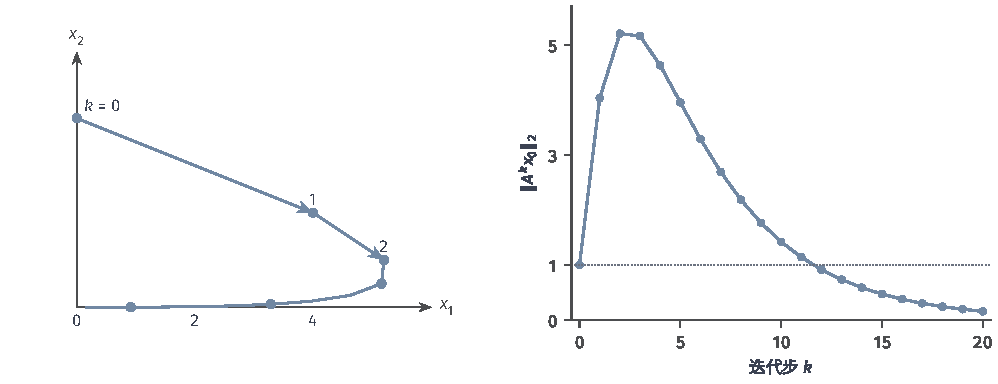
\includegraphics[width=169.0mm]{figures/01-mathematical-preliminaries-upper/02-linear-spaces/matplotlib/ch06-transient-growth/figure.pdf}
  \caption{固定二维矩阵的反复作用。初值为$(0,1)^{\top}$，前两步的长度增加，
  此后回到原点；右图将长度与初始长度$1$比较。特征值$0.8$和$0.5$决定长期衰减，
  非正交特征方向间的相消则决定早期放大。两图使用同一个矩阵和同一组迭代点。}
  \label{fig:ch06-transient-growth}
\end{figure*}

该矩阵可对角化，特征向量$\bm v_1=(1,0)^{\top}$、$\bm v_2=(-40/3,1)^{\top}$
对应$0.8$和$0.5$，因而
\begin{equation}
 \bm A^k=
 \begin{bmatrix}
  0.8^k&\frac{40}{3}(0.8^k-0.5^k)\\
  0&0.5^k
 \end{bmatrix},\qquad
 \bm x^{(k)}=
 \begin{bmatrix}\frac{40}{3}(0.8^k-0.5^k)\\0.5^k\end{bmatrix}.
 \label{eq:ch06-diagonalizable-finite-trajectory}
\end{equation}
$k=1,2,3$分别给$(4,0.5)^{\top}$、$(5.2,0.25)^{\top}$、$(5.16,0.125)^{\top}$，
与逐步相乘一致。初值实际写成$\tfrac{40}{3}\bm v_1+\bm v_2$，两个大横向分量
初始相消；衰减速度不同使相消被打破，长度先增大后回落。

\subsubsection{谱结构与增长速度}

\paragraph{特征方向不足与广义特征链}

当几何重数小于代数重数时，独立特征向量张不满空间，需要广义特征向量补齐：
对正整数$j$满足$(\bm A-\lambda\bm I)^j\bm v=\bm0$的非零向量。一条链从特征
向量$\bm v_1$开始，后续满足$(\bm A-\lambda\bm I)\bm v_{j+1}=\bm v_j$，
减去共同缩放后每个方向被送到链中前一个方向。动机：仅有的几个特征方向无法
分解任意初值，而幂$\bm A^k$沿链逐级平移，必须知道链长才能解释多项式增长。
复算：$\bm J=\begin{smallmatrix}0.8&1\\0&0.8\end{smallmatrix}$只有一个
特征向量$(1,0)^{\top}$，初值$(0,1)^{\top}$不在其中，若只按特征方向分解
就会漏掉第二坐标的耦合项。

\paragraph{实分裂条件下的Jordan块}

本节只处理特征多项式实分裂的情形（全部特征值为实数），非实共轭对留给实Schur块。
在链基下矩阵由块$\bm J_s(\lambda)=\lambda\bm I+\bm N$组成，$\bm N$为
$s\times s$幂零矩阵、$\bm N^s=\bm0$，超对角元为$1$。相似变换
$\bm J_s=\bm P^{-1}\bm A\bm P$保持谱与幂的长期行为（$\bm A^k=
\bm P\bm J_s^k\bm P^{-1}$），所以块分析可直接用于原矩阵。这是相似分类的
标准形，用于解释结构，数值计算通常不主动构造对扰动极敏感的链基。

\paragraph{链长度与相似分类}

块大小$s$等于该$\lambda$对应的最长链长度，即代数重数减去几何重数后的耦合深度。
$s=1$是普通特征方向；$s>1$记录“缺少独立特征方向”。例如
$\begin{smallmatrix}0.8&1\\0&0.8\end{smallmatrix}$只有一个特征方向，
不能因为对角元相同就当作$0.8\bm I$：后者可对角化、幂直接是$0.8^k\bm I$，
前者幂含$k0.8^{k-1}$耦合项，长期速度虽同为指数衰减，有限步轨迹不同。
判别方法：解$(\bm A-0.8\bm I)\bm v=0$只得到一维解空间，几何重数为$1$、
代数重数为$2$，故必有$s=2$块。

\paragraph{块幂中的多项式增长因子}

对$\bm J=\lambda\bm I+\bm N$作二项式展开（$\lambda\bm I$与$\bm N$可交换），
\begin{equation}
 \bm J^k=\sum_{j=0}^{\min(k,s-1)}\binom{k}{j}\lambda^{k-j}\bm N^j,
 \qquad k=0,1,\ldots.
 \label{eq:ch06-jordan-power}
\end{equation}
$\lambda=0$时$\bm J^k=\bm N^k$，$k\geq s$后恰为零（幂零）；$\lambda\neq0$时
$\binom{k}{j}$提供至多$s-1$次的多项式因子，而整体仍带$\lambda^k$指数。以
$\bm J=\begin{bmatrix}0.8&1\\0&0.8\end{bmatrix}$为例，
$\bm J^k=\begin{bmatrix}0.8^k&k\,0.8^{k-1}\\0&0.8^k\end{bmatrix}$，
初值$(0,1)^{\top}$第一步成为$(1,0.8)^{\top}$、第二步成为$(1.6,0.64)^{\top}$；
第一坐标的累积项$k0.8^{k-1}$先上升（$k\approx5$附近达到约$2.05$）再由指数
衰减主导。图~\ref{fig:vol1-add-linear-jordan-accumulation}画出两个坐标的
逐步变化。边界：多项式因子永远压不过$|\lambda|^k$，所以$\rho<1$时块幂
仍趋零，只是比对角情形慢一个多项式阶；$\rho=1$且$\lambda=1$的$s>1$块则
线性发散。

\begin{figure}[!htb]
  \centering
  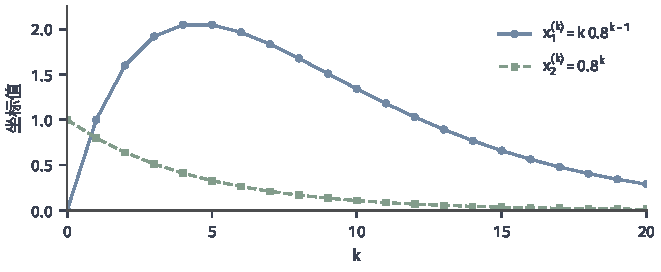
\includegraphics[width=112mm]{figures/01-mathematical-preliminaries-upper/02-linear-spaces/matplotlib/comprehension-additions/linear-jordan-accumulation.pdf}
  \caption{Jordan块的累积项。取正文$\bm J=\left[\begin{smallmatrix}0.8&1\\0&0.8\end{smallmatrix}\right]$与初值$(0,1)^{\top}$。绿线为$0.8^k$，蓝线在$k\geq1$时为$k0.8^{k-1}$，在$k=0$时为$0$。点表示整数步，连线仅引导读图；两坐标最终都趋零。}
  \label{fig:vol1-add-linear-jordan-accumulation}
\end{figure}

若$\bm A=\bm V\bm\Lambda\bm V^{-1}$实可对角化，对定义在其谱上的单值函数$f$，
\begin{equation}
 f(\bm A)=\bm V\operatorname{diag}(f(\lambda_1),\ldots,f(\lambda_d))\bm V^{-1}.
 \label{eq:matrix-analysis-matrix-function-diagonalizable}
\end{equation}
不可对角化时仅给根上的函数值不够，还要块大小所需的导数：
\begin{equation}
 f(\bm J_s(\lambda))=\sum_{j=0}^{s-1}\frac{f^{(j)}(\lambda)}{j!}\bm N^j,
 \label{eq:ch06-jordan-function}
\end{equation}
这是Taylor展开在$\bm N^s=\bm0$后精确终止的结果。证明：把$f$在$\lambda$处
展开，$(\bm J_s-\lambda\bm I)=\bm N$，高阶项$\bm N^j$在$j\geq s$为零，
逐项代入即得。函数中的多项式因子$t^j/j!$不是数值近似误差，而是幂零耦合的
真实作用；$f$在$\lambda$处不可导时，Jordan块上的$f(\bm A)$无法良好定义。

\paragraph{实Schur块与旋转衰减}

一般实矩阵取实Schur形式，$\bm Q$正交，$\bm T$为分块上三角，对角块大小为
$1$或$2$：
\begin{equation}
 \bm A=\bm Q\bm T\bm Q^{\top},\qquad \bm Q^{\top}\bm Q=\bm I.
 \label{eq:matrix-analysis-schur-decomposition}
\end{equation}
$2\times2$块对应非实共轭特征值对，形如
$\begin{bmatrix}a&-b\\b&a\end{bmatrix}=r\!\begin{bmatrix}\cos\theta&-\sin\theta\\\sin\theta&\cos\theta\end{bmatrix}$，
其幂为$r^k$乘旋转$k\theta$，$r=\sqrt{a^2+b^2}=|\lambda|$；
$r<1$时旋转振荡地衰减，$r=1$时在圆周上匀速旋转不取极限，$r>1$时增长。
上三角耦合项在块稳定时被几何因子吸收：把块按$r^k$归一，耦合贡献含额外
$r^k$因子，长期可忽略。

\paragraph{特征基条件与瞬态放大}

可对角化但非正交时，
\[
\lVert\bm A^k\rVert_2\leq
\lVert\bm V\rVert_2\lVert\bm V^{-1}\rVert_2\max_i|\lambda_i|^k,
\]
坐标放大因子$\lVert\bm V\rVert\lVert\bm V^{-1}\rVert$进入有限步界，它只在
$k$大时被$\max|\lambda_i|^k$压过，早期不受谱控制。自伴情形$\bm V$可取
正交，该因子为$1$；非正交基不能忽略它，这正是上面二维例短时放大的来源。
边界：该界是上界，非正交基病态时实际早期长度可能更大，但长期衰减率仍由
$\rho$决定，二者不矛盾。

\paragraph{分析表示和数值表示的区别}

Jordan形式用于解释结构和证明速度，微小扰动就可能改变块结构（把一个$s=2$块
拆成两个近邻特征值），数值识别精确块并不稳健；实际计算采用Schur形式只处理
稳定的分块上三角，不主动构造链基。分析结论（$\rho<1$趋零）与数值实现
（避免病态基）分工明确：证明用Jordan链说明多项式因子，工程计算用Schur块
避免对扰动敏感的基变换。

\subsubsection{非负矩阵的反复作用}

\paragraph{非负作用与质量传递}

逐项非负的$\bm A\geq0$（每个元素$a_{i,j}\geq0$）把非负向量$\bm x\geq0$映为
非负向量$\bm A\bm x\geq0$，分量之间只转移不创造。把$\bm x$看作各通道的质量，
$(\bm A\bm x)_i=\sum_j a_{i,j}x_j$是从$j$流入$i$的总量，$\bm A^k\bm x$描述
经过$k$步传递后的分布。非负性使各分量不会因相消变号，因而可以用分量比值
（而非范数）刻画方向收敛，这是Perron理论比一般谱分析更精细的原因。本小节只做
代数的收敛分析，概率转移的随机解释留待概率卷。

\paragraph{正矩阵的比值极值与正特征方向}

正矩阵（所有元素严格为正）满足Perron--Frobenius理论的最干净情形：谱半径
$\rho(\bm A)$本身是一个正特征值，对应一个严格为正的特征向量，且模不超过
$\rho(\bm A)$的其他特征值都不可能与之并列主导\scite{math-horn2013matrix}。
Collatz--Wielandt比值检验给出存在性与上下界：对任意正向量$\bm x>0$取
$m(\bm x)=\min_i(\bm A\bm x)_i/x_i$与$M(\bm x)=\max_i(\bm A\bm x)_i/x_i$，
则$m(\bm x)\leq\rho(\bm A)\leq M(\bm x)$。证明要点：设$\bm p>0$为Perron
方向、$\bm A\bm p=\rho\bm p$，令$s=\min_i x_i/p_i$、$t=\max_i x_i/p_i$，
则$\bm x\geq s\bm p$、$\bm x\leq t\bm p$，由非负性$\bm A\bm x\geq s\rho\bm p$
给出$m(\bm x)\geq s\rho$，$\bm A\bm x\leq t\rho\bm p$给出$M(\bm x)\leq t\rho$，
两式相除并取遍分量即得夹逼。复算正矩阵$\bm P=\begin{smallmatrix}1&2\\3&4\end{smallmatrix}$，
$\rho(\bm P)=(5+\sqrt{33})/2\approx5.3723$；取正向量$\bm x=(1,1)^{\top}$，
$\bm P\bm x=(3,7)^{\top}$，比值$m=3\leq5.3723\leq M=7$。再作用一次
$\bm P^2\bm x=(17,37)^{\top}$，比值区间收紧到$[5.286,5.667]$，第三步
$[5.353,5.378]$，逐次夹到$\rho$，演示区间单调收紧。反复作用$\bm A^k\bm x$时比值区间
$[m(\bm A^k\bm x),M(\bm A^k\bm x)]$单调收紧到$\rho(\bm A)$。
适用条件：$\bm A$不可约（本原矩阵更直接）且初值$\bm x>0$为正向量；
证明收紧方向：每作用一次，比值区间被夹逼关系重新包裹，$s,t$随$\bm A^k\bm x$
趋于Perron方向而收敛到同一比值，故区间两端收敛到$\rho$。边界：可约矩阵或
初值在某对角块上投影为零时，区间可能卡在该块的Perron根而不收紧到整矩阵的
$\rho$，不能把夹逼结论无条件外推。

\paragraph{非负逼近与不可约条件}

元素含零的非负矩阵要先区分连通性：把下标看作有向图的顶点，$a_{i,j}>0$即从$j$到$i$
有边，\term{不可约}（irreducible）指该图强连通，任意两顶点间有正向路径。
可约矩阵可经置换写成块上三角，各对角块独立传递，整矩阵的主方向由各块比较决定，
不能直接套用正矩阵结论。复算：$\bm A=\operatorname{diag}(0.5,0.8)$可约，
两个块各有自己的Perron根，长期方向由较大的$0.8$块决定，另一块分量直接衰减，
不存在全体正的公共主方向。

\paragraph{Perron根与主方向的尺度}

不可约非负矩阵仍有$\rho(\bm A)>0$作为一个单特征值（代数重数为$1$），对应
严格正的Perron方向$\bm p>0$；但其他特征值可以具有同一模$|\lambda|=\rho(\bm A)$，
此时长期行为不是单一方向。$\bm p$只在相差一个正倍数的意义下确定，归一化
（除以分量和或长度）去掉任意尺度。条件要点：上述正Perron方向与单重性要求
不可约；可约矩阵的Perron根可能多重，且主方向只在主导块内为正。

\paragraph{正幂下的收缩与归一化极限}

不可约且\term{本原}（primitive），即存在$k_0$使$\bm A^{k_0}>0$（某一幂把所有
零位置填正），则其余特征值的模都严格小于$\rho(\bm A)$。于是对任意非零
$\bm x\geq0$，归一化幂序列
$\bm A^k\bm x/\lVert\bm A^k\bm x\rVert$收敛到Perron方向；未归一化时
$\bm A^k\bm x$按$\rho(\bm A)^k$增长或衰减，方向先于尺度稳定。证明要点：
把$\bm x$在特征基展开，主导项为$\rho^k c\bm p$，其余项按$|\lambda_j|^k$
（$|\lambda_j|<\rho$）衰减，除以$\rho^k$后余项趋零，方向趋于$\bm p$。
初值条件：$\bm x\geq0$且不含零分量在主导块上的投影为零；本原性保证
$\bm A^{k_0}>0$把任何非零非负初值都变成正向量，故初值限制很弱。

\paragraph{周期情形的振荡边界}

不可约但非本原的矩阵有周期$p>1$：存在$p$个模同为$\rho(\bm A)$的特征值，
均匀分布在半径$\rho(\bm A)$的圆周上（实矩阵中成共轭对出现）。归一化序列在$p$个
循环类之间轮换，$k$模$p$不同时落在不同方向，不存在单一极限；这是
$\rho(\bm A)=1$边界振荡在非负矩阵中的具体形态。复算：$p=2$的置换矩阵
$\begin{smallmatrix}0&1\\1&0\end{smallmatrix}$，$\bm A^k$在$\bm I$与$\bm A$间
交替，归一化方向轮换，永不收敛到固定向量。

\paragraph{随机矩阵的代数保持与概率入口}

行和（或列和）全为$1$的非负矩阵称为\term{随机矩阵}（stochastic matrix），
代数上它保持总质量：$\sum_i(\bm A\bm x)_i=\sum_jx_j$（行和口径，因为
$\sum_i a_{i,j}=1$），$\rho(\bm A)=1$且$1$为特征值。本原随机矩阵的归一化
分布收敛到平稳Perron方向，这里只用到质量保持与方向收敛；“分布收敛到平稳分布”
的概率论证（遍历性、期望收敛）属于概率卷，这里不展开。边界：可约随机矩阵
存在多个闭类，初值落在哪个闭类就收敛到哪个平稳分布，不存在全体初值的公共极限。

\subsubsection{变化矩阵的连乘}

\paragraph{变化矩阵与有序乘积}

迭代中每步矩阵可能不同，第 $k$ 步乘积写成 $\bm B_k\cdots\bm B_1\bm x^{(0)}$，
误差按同一顺序累积。与固定矩阵不同，每一步的谱半径都小于$1$并不能保证乘积
衰减，因为各步作用的方向不一致：$\rho(\bm B_j)<1$只描述$\bm B_j$自身的
长期行为，而乘积的早期放大由各步方向间的夹角决定，谱半径不携带这一信息；
必须用乘积整体控制，不能逐步检查谱半径。

\paragraph{逐步谱半径不足的例子}

取$\bm B_1=\begin{bmatrix}0&2\\0&0\end{bmatrix}$、
$\bm B_2=\begin{bmatrix}0&0\\2&0\end{bmatrix}$，二者$\rho=0$且都是幂零的，
但$\bm B_2\bm B_1=\operatorname{diag}(0,4)$把第二分量放大$4$倍。
逐步相乘复算：$\bm B_1$把$(x_1,x_2)^{\top}$映为$(2x_2,0)^{\top}$，
$\bm B_2$再映为$(0,2\cdot2x_2)^{\top}=(0,4x_2)^{\top}$。
单个矩阵没有非零谱，两步交换方向后却产生放大，说明必须用乘积整体控制，
不能逐步检查谱半径。

\paragraph{共同范数与一致收缩}

若存在同一个范数使所有$\lVert\bm B_k\rVert\leq q<1$（一致收缩），则
$\lVert\bm B_k\cdots\bm B_1\rVert\leq q^k$，任意初值误差按几何因子$q^k$衰减。
关键是“同一个范数、同一个上界”；每步换范数或上界随$k$接近$1$，结论都不成立。
证明由次乘性归纳：$\lVert\bm B_k\cdots\bm B_1\rVert\leq
\lVert\bm B_k\rVert\lVert\bm B_{k-1}\cdots\bm B_1\rVert\leq q\cdot q^{k-1}$。

\paragraph{连乘界与初值误差衰减}

由次乘性递推，
$\lVert\bm e^{(k)}\rVert\leq\lVert\bm B_k\rVert\cdots\lVert\bm B_1\rVert
\lVert\bm e^{(0)}\rVert$。一致收缩时该乘积$\leq q^k\lVert\bm e^{(0)}\rVert$，
初始误差被整体压小，不需要逐坐标跟踪。边界：若仅$\lVert\bm B_k\rVert\leq1$
而无统一$q<1$，只能得到有界，不能推出趋零；若各步上界$q_k\to1$，乘积
$\prod q_k$可能不趋零。

\paragraph{作用顺序与累计放大}

矩阵不可交换，顺序不能随意调换：上例中$\bm B_1\bm B_2=\operatorname{diag}(4,0)$
放大的是第一分量。复算：$\bm B_2$先把$(x_1,x_2)^{\top}$映为$(0,2x_1)^{\top}$，
$\bm B_1$再映为$(2\cdot2x_1,0)^{\top}=(4x_1,0)^{\top}$。连乘界按实际作用
顺序相乘，重排步序会改变放大方向，比较两种实现时必须保留各自顺序。

\paragraph{缺少共同控制时的边界}

不存在共同一致收缩界时，乘积可能在某段内放大，是否长期收敛需要联合结构
（共同不变度量、联合谱半径等），超出本卷范围；本卷只要求识别“逐步谱半径小”
不是充分条件这一边界，不为变化矩阵编造统一衰减保证。

\subsection{矩阵级数与指数演化}
\label{sec:ls-matrix-series-exponential}

\subsubsection{矩阵级数}

\paragraph{部分和与尾项误差}

矩阵幂级数$\sum_{k=0}^{\infty}\bm A^k$的第$N$部分和
$\bm S_N=\sum_{k=0}^N\bm A^k$；级数收敛指$\bm S_N$作为矩阵序列收敛。
尾项$\sum_{k>N}\bm A^k$就是部分和与极限的差距，需要可计算的尾界而不是
只看通项趋零。动机：通项$\bm A^k\to0$只是级数收敛的必要条件，标量级数
$\sum 1/k$通项趋零却发散，矩阵级数同样不能仅凭通项判断；截断到$N$步时
必须给出尾项范数上界才能报告近似精度。

\paragraph{幂衰减下的Neumann收敛}

\term{Neumann级数}（Neumann series）$\sum_{k=0}^{\infty}\bm A^k$在
$\lVert\bm A\rVert<1$（某次乘性范数）时收敛。这是绝对收敛：
$\sum_k\lVert\bm A^k\rVert\leq\sum_k\lVert\bm A\rVert^k<\infty$，
由有限维范数等价保证矩阵级数绝对收敛即收敛。证明：绝对收敛的矩阵级数其
每个元素都是绝对收敛的标量级数，有限个元素同时收敛，故部分和矩阵收敛。

\paragraph{部分和恒等式与逆的构造}

逐项相消恒等式
$(\bm I-\bm A)\sum_{k=0}^N\bm A^k=\bm I-\bm A^{N+1}$，直接展开左侧：
$\sum_{k=0}^N\bm A^k-\sum_{k=1}^{N+1}\bm A^k=\bm I-\bm A^{N+1}$。
$\lVert\bm A\rVert<1$时$\bm A^{N+1}\to\bm0$，令$N\to\infty$得
$(\bm I-\bm A)\sum_{k=0}^{\infty}\bm A^k=\bm I$，故$\bm I-\bm A$可逆且
\begin{equation}
 (\bm I-\bm A)^{-1}=\sum_{k=0}^{\infty}\bm A^k.
 \label{eq:ls-neumann-series}
\end{equation}
右侧同样给出$(\sum\bm A^k)(\bm I-\bm A)=\bm I$，左逆即右逆。这是用级数
构造逆的显式公式，也给出逆的存在性充分条件；复算标量$\bm A=0.5$时
$(1-0.5)^{-1}=2=1+0.5+0.25+\cdots$，与几何级数一致。

\paragraph{几何尾界的范数条件}

尾项满足
$\lVert\sum_{k>N}\bm A^k\rVert\leq
\sum_{k>N}\lVert\bm A\rVert^k=
\lVert\bm A\rVert^{N+1}/(1-\lVert\bm A\rVert)$，
可直接用于截断误差估计。条件写为$\lVert\bm A\rVert<1$是充分的；
谱半径$\rho(\bm A)<1$时由~\ref{sec:ls-matrix-power-behavior}节分块估计仍可收敛，
但要先换到一个使范数上界小于$1$的等价范数，不能直接使用原范数尾界。
边界：$\lVert\bm A\rVert=1$时几何尾界分母为零，给不出衰减；$\rho(\bm A)<1$
而原范数$\geq1$时级数仍收敛，只是尾界需换范数后重算。

\paragraph{一般幂级数的收敛范围}

对标量幂级数$f(s)=\sum_{k=0}^{\infty}a_ks^k$的收敛半径$R$，矩阵级数
$\sum_{k=0}^{\infty}a_k\bm A^k$在$\rho(\bm A)<R$时收敛；$\rho(\bm A)>R$
发散，$\rho(\bm A)=R$边界上逐项判断。Jordan块中的多项式因子被$R^{-k}$吸收，
不改变收敛半径。复算：$f(s)=1/(1-s)$的$R=1$，对应Neumann级数；
$f(s)=e^s$的$R=\infty$，所以矩阵指数对任意$\bm A$收敛。

\paragraph{离散Lyapunov级数的构造}

离散时间稳定传播$\bm x^{(t+1)}=\bm A\bm x^{(t)}$下，正定Gram量
$\bm P=\sum_{k=0}^{\infty}(\bm A^{\top})^k\bm Q\bm A^k$（$\bm Q\succeq0$）
是离散Lyapunov方程
$\bm P-\bm A^{\top}\bm P\bm A=\bm Q$的解。把级数代入：
$\bm P-\bm A^{\top}\bm P\bm A=\bm Q+\sum_{k\geq1}(\bm A^{\top})^k\bm Q\bm A^k-
\sum_{k\geq0}(\bm A^{\top})^{k+1}\bm Q\bm A^{k+1}=\bm Q$，逐项相消。
级数收敛的条件正是$\rho(\bm A)<1$，每一项按$\rho^{2k}$量级衰减，级数
才有意义；该级数也是误差协方差在稳定传播下的长期累积。

\paragraph{正定性、唯一性与稳定条件}

$\bm Q\succ0$且$\bm A$稳定时$\bm P\succ0$：对任意非零$\bm x$，
$\bm x^{\top}\bm P\bm x=\sum_k(\bm A^k\bm x)^{\top}\bm Q(\bm A^k\bm x)>0$，
至少$k=0$项为正且其余非负。$\bm Q\succeq0$时$\bm P\succeq0$。
齐次方程$\bm P-\bm A^{\top}\bm P\bm A=0$在$\rho(\bm A)<1$时只有零解，
故级数给出唯一正定解：迭代$\bm P_{k+1}=\bm A^{\top}\bm P_k\bm A+\bm Q$
收敛到该解。连续时间的积分构造$\bm P=\int_0^\infty e^{\bm A^{\top} t}\bm Qe^{\bm At}dt$
留待微分方程章，此处不重复。

\subsubsection{矩阵指数}

\paragraph{固定时刻的级数与截断误差}

矩阵指数$e^{t\bm A}=\sum_{k=0}^{\infty}(t\bm A)^k/k!$的定义、收敛半径
（整函数，任意$\rho(\bm A)$都收敛）与级数计算已在
~\ref{sec:ls-matrix-exponential}节建立，这里不重复定义。
本小节只分析$t\to\infty$的长期行为：固定$t$的截断误差由级数尾界估计，
与时间趋于无穷是两个独立问题，前者靠$k!$压任意$(t\lVert\bm A\rVert)^k$，
后者由谱实部决定。

\paragraph{时间趋于无穷的独立问题}

$e^{t\bm A}$在每个有限$t$都存在且可逆（逆为$e^{-t\bm A}$），不意味着
$t\to\infty$趋零；长期行为由谱的实部（实矩阵对应Schur块的$a$）决定，
与级数是否收敛无关。动机：级数对所有$t$收敛只保证“每个时刻有定义”，
不保证轨迹衰减，必须单独检查特征值实部符号；固定$t$的级数存在与
$t\to\infty$行为是两个独立问题。

\paragraph{实对称谱下的衰减、保持与增长}

$\bm A$实对称时$e^{t\bm A}=\bm Q\operatorname{diag}(e^{t\lambda_i})\bm Q^{\top}$。
$\lambda_i<0$方向$e^{t\lambda_i}\to0$衰减；$\lambda_i=0$方向保持；
$\lambda_i>0$方向指数增长。三类方向由初值分量决定取舍，不能只报一个最大实部。
复算：$\bm A=\operatorname{diag}(-1,0,1)$，初值含第三分量时第三分量
$e^t$发散，前两分量分别衰减、保持，整体发散与前两分量无关。

\paragraph{实Schur块中的振荡和耦合}

一般实矩阵的$2\times2$块$\begin{bmatrix}a&-b\\b&a\end{bmatrix}$是缩放$r$乘
旋转，其指数为$e^{at}$乘旋转角$bt$：实部$a<0$时$e^{at}$旋转振荡地衰减，
$a=0$纯旋转保持长度，$a>0$增长。上三角耦合项在块稳定时被$e^{at}$吸收，
不改变主振荡频率。复算：$a=-1,b=2$时块指数为$e^{-t}$乘旋转$2t$，
长度$e^{-t}$趋零而方向持续振荡，两者同时发生。

\paragraph{非正规作用下的短期放大}

与矩阵幂同理，非正规矩阵$e^{t\bm A}$在早期可能因非正交方向相消而放大，
即使谱实部全为负、长期趋零。短期界由$\lVert e^{t\bm A}\rVert$的
有限步估计给出，长期由谱实部决定，二者分开报告；不得用
$e^{t\max\operatorname{Re}\lambda}$直接当作前几步长度上界。

\paragraph{长期界与初始方向}

$t\to\infty$时$e^{t\bm A}$的极限行为由最大实部特征空间主导，初值在该子空间的
分量决定长期残留；衰减方向的贡献只出现在有限时间内。若初值恰好不含最大实部
方向分量，主导项由次大实部给出，报告长期速度必须先检查初值投影。

\subsection{定常迭代的收敛}
\label{sec:ls-stationary-convergence}

~\ref{sec:ls-stationary-iterations}节给出分裂$\bm A=\bm M-\bm N$与四种定常
格式的更新公式，本节只证明
误差序列何时趋零、按什么因子趋零，不再重复逐行实现。

\subsubsection{一般判据}

\paragraph{分裂更新与精确解之差}

设$\bm x_*$满足$\bm A\bm x_*=\bm b$，迭代$\bm M\bm x^{(t+1)}=\bm N\bm x^{(t)}+\bm b$。
误差$\bm e^{(t)}=\bm x^{(t)}-\bm x_*$满足
$\bm M\bm e^{(t+1)}=\bm N\bm e^{(t)}$：把$\bm x^{(t+1)}=\bm e^{(t+1)}+\bm x_*$、
$\bm x^{(t)}=\bm e^{(t)}+\bm x_*$代入，利用$\bm M\bm x_*=\bm N\bm x_*+\bm b$
消去精确解项，右端$\bm b$随之消失，所以误差递推与右端无关。

\paragraph{误差传播矩阵的形成}

记误差传播矩阵$\bm T=\bm M^{-1}\bm N$，则
$\bm e^{(t+1)}=\bm T\bm e^{(t)}$，归纳得
$\bm e^{(t)}=\bm T^t\bm e^{(0)}$。迭代是否收敛完全由$\bm T^t$决定，
与右端$\bm b$无关；这也意味着换一个右端不改变收敛速度，只改变初始误差。
推导：由$\bm M\bm e^{(t+1)}=\bm N\bm e^{(t)}$两边左乘$\bm M^{-1}$即得
$\bm T=\bm M^{-1}\bm N$。

\paragraph{所有初值收敛的谱判据}

\begin{theorem}[定常迭代的收敛判据]
\label{thm:ls-stationary-convergence}
对任意初值$\bm x^{(0)}$都有$\bm x^{(t)}\to\bm x_*$，当且仅当
$\rho(\bm T)<1$。
\end{theorem}
\begin{proof}
必要性：若存在特征值$|\lambda|\geq1$及对应特征向量$\bm v$，取
$\bm e^{(0)}=\bm v$，则$\bm e^{(t)}=\lambda^t\bm v$不趋零。
充分性：$\rho(\bm T)<1$由~\ref{thm:ls-power-decay}得$\bm T^t\to0$，
故$\bm e^{(t)}\to0$。
\end{proof}
该判据是~\ref{sec:ls-matrix-power-behavior}节固定矩阵幂判据的直接应用；$\rho(\bm T)<1$是对全体初值收敛的
充要条件，任何范数上界（如$\lVert\bm T\rVert<1$）只是更保守的充分条件。

\paragraph{渐近速度与有限步界}

渐近速度由$\rho(\bm T)$给出：误差最终按$\rho(\bm T)^t$量级下降。
有限步则用$\lVert\bm T^t\rVert$估计，非正规的$\bm T$可能在前几步放大，
$\lVert\bm T^t\rVert\leq C_r r^t$（$r>\rho(\bm T)$）保留了这一可能；
不能用$\rho(\bm T)^t$直接当作前几步的误差界。复算：$\rho(\bm T)=0.8$
但$\bm T$非正交时第一步$\lVert\bm T\bm e^{(0)}\rVert$可能大于$\lVert\bm e^{(0)}\rVert$，
长期仍按$0.8^t$下降。

\paragraph{残差和误差的关系}

精确解满足$\bm r^{(t)}=\bm b-\bm A\bm x^{(t)}=-\bm A\bm e^{(t)}$，
故$\bm e^{(t)}=-\bm A^{-1}\bm r^{(t)}$。残差小不直接等于误差小，二者之间隔
着$\bm A^{-1}$的放大，定量条件界属~\ref{sec:ls-perturbation}节；本节只要求停止时
同时重算原残差，不用递推残差代替。

\subsubsection{Richardson迭代}

\paragraph{正定谱方向中的误差递推}

$\bm A$对称正定（SPD），取$\bm A=\bm Q\operatorname{diag}(\lambda_i)\bm Q^{\top}$，
Richardson更新$\bm x^{(t+1)}=\bm x^{(t)}+\omega\bm r^{(t)}$给出
$\bm e^{(t+1)}=(\bm I-\omega\bm A)\bm e^{(t)}$。在特征方向上误差解耦为
$e_i^{(t+1)}=(1-\omega\lambda_i)e_i^{(t)}$，每个方向独立按标量因子衰减；
因为$\bm A$自伴，不同特征方向不耦合，可逐方向检查倍率。

\paragraph{各方向同时收缩的步长范围}

要所有方向$|1-\omega\lambda_i|<1$，即$-1<1-\omega\lambda_i<1$。
由$\lambda_i>0$得右不等式自动成立（$\omega>0$），左不等式给
$\omega<2/\lambda_{\max}(\bm A)$，故谱口径的收敛区间为
$0<\omega<2/\lambda_{\max}$。6.2 节的算子范数口径把可执行条件写成
$0<\omega<2/\lVert\bm A\rVert_2$；对称正定时$\lVert\bm A\rVert_2=
\lambda_{\max}(\bm A)$（诱导欧氏范数等于最大特征值），两个口径一致，
前者用谱判据证明全体方向收敛，后者用范数直接核验。

\paragraph{极端特征值控制的最坏因子}

最慢方向由最小、最大特征值两端控制：最坏因子
$q_\omega=\max_i|1-\omega\lambda_i|$只出现在$\lambda_{\min}$或
$\lambda_{\max}$，中间特征值不会给出更大的绝对值，因为$|1-\omega\lambda|$
在正区间上是$|\lambda-\tfrac1\omega|$的单调函数，最大值在端点。

复算$\bm A=\operatorname{diag}(1,3)$、$\omega=0.5$时两端因子为$0.5$与$-0.5$，中间无其他特征值；若存在$\lambda=2$，因子$0$更小，不参与最坏。

\paragraph{最优固定步长的平衡}

把两端拉到同一水平：$1-\omega\lambda_{\min}=-(1-\omega\lambda_{\max})$，
解得$\omega_*=2/(\lambda_{\min}+\lambda_{\max})$，
最优最坏因子
$q_*=(\lambda_{\max}-\lambda_{\min})/(\lambda_{\max}+\lambda_{\min})
=(\kappa-1)/(\kappa+1)$，$\kappa=\lambda_{\max}/\lambda_{\min}$。
复算$\bm A=\operatorname{diag}(1,3)$时$\omega_*=1/2$，
$q_*=1/2$，两端因子分别为$1/2$和$-1/2$。

\paragraph{条件数与收敛速度}

$\kappa$大时$q_*\approx1-2/\kappa$，收敛极慢；谱集中在窄区间时$q_*$接近$0$。
固定步长的速度由条件数决定，条件数改善（预条件）的定量作用见
~\ref{sec:ls-preconditioning}节预条件构造。复算$\kappa=100$时
$q_*\approx0.98$，约需百步量级才压缩一个数量级。

\paragraph{步长端点的边界行为}

$\omega\to0$时因子$1-\omega\lambda_i\to1$，几乎不动；端点
$\omega=2/\lambda_{\max}$使最大方向因子为$-1$，误差在该方向交替符号而长度
不减、不衰减；区间外某方向$|1-\omega\lambda_i|>1$，该分量几何增长，整列发散。
端点与区间外都不给出收敛，必须严格落在开区间$(0,2/\lambda_{\max})$内。

\subsubsection{Jacobi迭代}

\paragraph{Jacobi误差矩阵}

记$\bm A=\bm D-\bm L-\bm U$（$\bm D$对角，$\bm L,\bm U$为严格下、上三角的
相反数），Jacobi迭代矩阵$\bm T_J=\bm D^{-1}(\bm L+\bm U)$，
误差$\bm e^{(t+1)}=\bm T_J\bm e^{(t)}$。它同时读取上一轮全部坐标，
不利用本轮新值，故$\bm T_J$固定，误差递推是定常的。

\paragraph{最大范数下的行和控制}

$\infty$范数诱导为最大行绝对值和：
$\lVert\bm T_J\rVert_\infty=
\max_i\sum_{j\neq i}|a_{i,j}|/|a_{i,i}|=:q$。
这是不需求特征值即可核验的充分收缩量，把每个坐标的新误差用旧误差最大值
线性放大。

复算：二阶对角占优矩阵$|a_{1,2}|/|a_{1,1}|=0.4$、$|a_{2,1}|/|a_{2,2}|=0.3$时$q=0.4<1$，无需特征值即可判定收缩；$q$只是上界，可能比真实$\rho(\bm T_J)$大。

\paragraph{严格对角占优与收缩}

各行严格对角占优即$q<1$，此时$\lVert\bm T_J\rVert_\infty<1$，
由次乘性$\lVert\bm e^{(t)}\rVert_\infty\leq q^t\lVert\bm e^{(0)}\rVert_\infty$，
迭代收敛。$q<1$是$\rho(\bm T_J)<1$的充分而非必要条件：存在$q\geq1$
但谱半径仍小于$1$的矩阵，此时范数界保守而迭代收敛。

边界：$q=1$（弱对角占优）时几何因子不严格小于$1$，给不出$q^t\to0$，只能另用谱判据；非严格占优矩阵仍可能$\rho(\bm T_J)<1$，但不能由行和推出。

\paragraph{由收缩得到误差界}

逐行写成$|e_i^{(t+1)}|\leq\sum_{j\neq i}|a_{i,j}|/|a_{i,i}|\,|e_j^{(t)}|
\leq q\lVert\bm e^{(t)}\rVert_\infty$，取最大行和即得上述$q^t$界，
不需要特征值计算；归纳：第$t$步取$i$使误差最大，即得
$\lVert\bm e^{(t)}\rVert_\infty\leq q\lVert\bm e^{(t-1)}\rVert_\infty$，
叠$t$次得$q^t$。

\paragraph{正定但不收敛的反例}

SPD不保证Jacobi收敛：取对角元为$1$、非对角元均为$0.9$的三阶正定矩阵，
写成$\bm A=0.1\bm I+0.9\bm J$（$\bm J$为全$1$矩阵），其特征值为
$2.8,0.1,0.1$（正定）。对角阵$\bm D=\bm I$，故Jacobi迭代矩阵
$\bm T_J=-\bm D^{-1}(\bm A-\bm D)=-0.9(\bm J-\bm I)$；$\bm J$的特征值为
$3,0,0$，故$\bm J-\bm I$的特征值为$2,-1,-1$，$\bm T_J$的特征值为
$-1.8,0.9,0.9$，$\rho(\bm T_J)=1.8>1$，一般初值发散。
因此“矩阵正定”不能直接推出Jacobi收敛，必须检查$\rho(\bm T_J)$或$q$；
这与Gauss--Seidel在SPD下必然收敛形成对照。

\subsubsection{Gauss--Seidel与SOR迭代}

\paragraph{坐标校正与二次能量变化}

SPD二次能量$\phi(\bm x)=\tfrac12\bm x^{\top}\bm A\bm x-\bm b^{\top}\bm x$，
第$i$坐标校正$\Delta x_i=\omega r_i/a_{i,i}$（$r_i=b_i-\sum_ja_{i,j}x_j$），
保持其余坐标不动，目标增量为
$-\dfrac{\omega(2-\omega)}{2a_{i,i}}r_i^2$。推导：把$\phi(x_i+\Delta x_i)$
在当前行展开，二次项$a_{i,i}\Delta x_i^2/2$、线性项$r_i\Delta x_i$合并，
代入$\Delta x_i=\omega r_i/a_{i,i}$即得该式。

\paragraph{Gauss--Seidel的一轮下降}

$\omega=1$时每一步增量为$-r_i^2/(2a_{i,i})<0$（$a_{i,i}>0$由SPD保证），
单坐标校正把$\phi$在该坐标方向最小化，$r_i=0$时增量为零、不再移动；
一轮顺序扫描后能量严格下降，已更新坐标立即供后续行使用，这是与Jacobi
同时读旧值的关键差别。

\paragraph{能量下界与坐标改变量趋零}

SPD的$\phi$有下界且强制（coercive），能量单调下降故收敛到有限极限；
总下降量$\sum_t\sum_i r_i^{(t)2}/a_{i,i}=\phi^{(0)}-\lim\phi^{(t)}<\infty$，
非负项级数收敛，通项$r_i^{(t)2}/a_{i,i}\to0$，即每步$r_i^{(t)}\to0$。
若某步残差不为零，该项为正，无限步累加将超过有限总下降量，矛盾。

\paragraph{残差趋零与误差恢复}

$r_i^{(t)}\to0$即$\bm r^{(t)}\to0$，由$\bm e^{(t)}=-\bm A^{-1}\bm r^{(t)}$
且有限维中$\bm A^{-1}$有界，$\lVert\bm e^{(t)}\rVert\leq
\lVert\bm A^{-1}\rVert\lVert\bm r^{(t)}\rVert\to0$。这证明SPD下
Gauss--Seidel收敛，而该保证不传给Jacobi，因为Jacobi一轮同时改动多个坐标，
单步能量展开不成立。

\paragraph{SOR参数对下降量的影响}

一般$\omega$时增量系数$\omega(2-\omega)/(2a_{i,i})$为正要求$0<\omega<2$；
在该区间内SOR每步同样下降，$\omega\neq1$只是改变每步移动幅度，不改变
下降方向。复算：$\omega=1$回到Gauss--Seidel；$\omega=0.5$与$\omega=1.5$
的系数$\omega(2-\omega)=0.75$对称，每步移动更慢但方向仍下降；$\omega=2$
系数为零、$\omega>2$系数为负，能量不再单调。快慢由谱结构而非单看$\omega$。

\paragraph{正定条件下的参数范围}

SPD且$0<\omega<2$时SOR收敛，闭环与Gauss--Seidel平行：单步增量为
$-\omega(2-\omega)r_i^2/(2a_{i,i})<0$，能量单调下降并有下界，故总下降量
$\sum_t\sum_i\omega(2-\omega)r_i^{(t)2}/(2a_{i,i})<\infty$；系数
$\omega(2-\omega)>0$可提出求和号，非负项级数收敛迫使$r_i^{(t)}\to0$，
再由$\lVert\bm e^{(t)}\rVert\leq\lVert\bm A^{-1}\rVert\lVert\bm r^{(t)}\rVert$
得$\bm e^{(t)}\to0$。因此在SPD下$0<\omega<2$也是SOR收敛的充分条件
（与上面的必要性合起来为充要）。Kahan必要条件是单向的：对一般矩阵，
SOR对任意初值收敛仅当$0<\omega<2$（收敛$\Rightarrow$区间内），反向不成立，
区间内仍可能不收敛，充分性需另行核验。在此区间内参数选择影响速度，最优$\omega_*$
依赖矩阵谱结构（如模型问题的超松弛最优值），不能无条件宣称超松弛一定更快。

\paragraph{参数选择与条件失效}

$\omega\leq0$或$\omega\geq2$时增量系数$\omega(2-\omega)\leq0$，能量不再
单调下降，不能再用本段能量论证证明收敛；$\omega$过大越过候选值可能振荡。
固定第$i$坐标的展开只证明单步下降，整体收敛仍以上述能量有界结合残差趋零完成。

\subsection{Krylov迭代的收敛}
\label{sec:ls-krylov-convergence}

~\ref{sec:ls-krylov-methods}节建立了Krylov子空间的生成与各方法的更新格式，
本节只证明误差或残差
多项式在谱上的衰减，不重复递推公式。

\subsubsection{CG与PCG}

\paragraph{能量误差的逐步最小化}

SPD方程$\bm A\bm x=\bm b$中，CG在$\bm x_0+\mathcal K_k(\bm A,\bm r_0)$内
最小化能量误差$\lVert\bm e\rVert_{\bm A}^2=\bm e^{\top}\bm A\bm e$，
故第$k$步能量误差不大于任何同空间候选的能量误差。动机：正规方程的极值条件
是$\bm A\bm e=-\bm r$，在仿射搜索空间内取能量最小等价于投影到解方向，
嵌套空间使这一最小值随$k$单调不增。

\paragraph{Krylov误差的多项式表示}

$\bm e_k=p_k(\bm A)\bm e_0$，其中$p_k$为次数至多$k$、$p_k(0)=1$的多项式
（由$\bm e_k=\bm e_0+\bm A\bm q_{k-1}(\bm A)\bm e_0$得到，常数项$1$来自
$p_k(0)=1$）。在$\bm A=\bm Q\operatorname{diag}(\lambda_i)\bm Q^{\top}$下，
每个特征方向的误差被$p_k(\lambda_i)$单独乘缩，因而问题化为“选次数$k$、
$p(0)=1$的多项式，使其在各$\lambda_i$上同时取小”。

\paragraph{谱区间上的Chebyshev界}

把谱限制在$[\lambda_{\min},\lambda_{\max}]$，次数$k$、$p(0)=1$的多项式在
该区间上的最大绝对值由Chebyshev多项式最小化，给出经典界
\begin{equation}
 \lVert\bm e_k\rVert_{\bm A}
 \leq 2\left(\frac{\sqrt{\kappa}-1}{\sqrt{\kappa}+1}\right)^k
 \lVert\bm e_0\rVert_{\bm A},
 \qquad \kappa=\frac{\lambda_{\max}}{\lambda_{\min}}.
 \label{eq:ch06-cg-condition-bound}
\end{equation}
证明要点：$p(t)=T_k((a+b-2t)/(b-a))/T_k((a+b)/(b-a))$在$[a,b]$上
$|p|\leq1$，利用$x>1$时$T_k(x)\approx(x+\sqrt{x^2-1})^k/2$得到
$(b-a)/(b+a)$相关的几何因子；$a=b$时$\bm A=a\bm I$，一步即解。

\paragraph{条件数与最坏速度估计}

该界只依赖$\kappa$，是最坏情形估计：$\kappa$大时因子接近$1$，能量误差下降慢；
它不承诺每步都按此因子下降，也不区分谱在区间内如何分布。复算$\kappa=100$
时Chebyshev因子$(\sqrt\kappa-1)/(\sqrt\kappa+1)\approx0.818$，每步只压缩约$18\%$，
与实际聚簇谱可能的骤降形成对比。注意这与7.2.4.2固定步长Richardson的最优因子
$q_*=(\kappa-1)/(\kappa+1)$不是同一量：$\kappa=10$时CG因子约$0.519$，而Richardson
的$q_*=9/11\approx0.82$，$\kappa=100$时分别为$0.818$与$0.980$；后者更接近$1$，
正是固定步长在病态矩阵上失效更快的定量原因，两套因子不可混用。

\paragraph{谱聚簇与实际收敛}

实际步数常远小于$d$：特征值聚成少数几个簇时，低次多项式在簇点上同时取小值，
误差在簇被“覆盖”后骤降。Chebyshev界只用区间端点，对聚簇过于保守，
报告速度时应区分最坏界与实际谱分布；把$d$个散开特征值误当成一个区间会
严重高估所需步数。复算：100个特征值聚成3个簇时，次数3—4的多项式即可在
各簇点同时取小，步数远小于$d$。

\paragraph{正定预条件与谱等价界}

PCG把SPD预条件$\bm M$用于对称等价系统$\bm M^{-1/2}\bm A\bm M^{-1/2}$，
其条件数$\kappa(\bm M^{-1/2}\bm A\bm M^{-1/2})$代入同一Chebyshev界；
非对称$\bm M^{-1}\bm A$不能当作自伴算子继承能量论证。预条件改善的是条件数，
不是改变原方程；预条件成本（构造、每次辅助求解、存储）应计入总代价。

\paragraph{有限步终止与有限精度}

精确算术下至多$d$步残差为零：满维空间中$d$个特征方向被多项式逐次消去，
这是不依赖步长调参的结构性质；初始误差为零时已经是精确解，不作额外限制。
有限精度中$\bm A$-共轭正交性逐步丢失，有限步终止不再成立，实际以真实残差
达到容限为准。

\subsubsection{MINRES}

\paragraph{嵌套子空间与残差最小化}

对称不定$\bm A$上MINRES在嵌套的$\mathcal K_k$中最小化欧氏残差
$\lVert\bm b-\bm A\bm x_k\rVert_2$，残差$\bm r_k=q_k(\bm A)\bm r_0$，
$q_k(0)=1$、次数至多$k$。不定矩阵没有正定能量可用，改用欧氏残差；
$\mathcal K_k$逐级嵌套，第$k$步最小值在更大空间取得，故残差范数单调不增。

\paragraph{对称谱上的残差多项式}

每个特征方向的残差分量被$q_k(\lambda_i)$乘缩；与CG在正定谱上最小化能量误差
$\bm e^{\top}\bm A\bm e$不同，MINRES目标是欧氏残差$\lVert\bm r\rVert_2$，
$\lambda_i$可正可负，多项式$q_k$要在整个实谱区间（含零点）上取小，
不能只在正区间逼近。

\paragraph{谱分布与残差衰减}

谱集中于少数区间时低次多项式可同时压低各点；谱跨越零点且分散时，
多项式逼近困难，残差下降慢。MINRES没有CG的条件数闭式因子，速度由谱分布决定。
复算$\bm A=\operatorname{diag}(-1,1)$时$q_k$需在$\pm1$同时取小，
低次多项式难以兼顾，残差下降慢于单符号谱；谱聚成少数点时低次多项式可同时压低。

\paragraph{相容性与有限步终止}

相容系统精确算术下至多$d$步残差为零：$\mathcal K_d$为全空间，第$d$步可取到
相容解使残差为零；残差单调不增（每步在更大空间取最小），这是MINRES相对
BiCGSTAB的结构保证，也是停止判断可以信任递推残差的原因。有限精度中正交性丢失，
该有限步结论不再严格成立。

\paragraph{奇异系统的残差和选解边界}

对称奇异且相容时MINRES给出最小残差解，但不保证最小欧氏范数代表；
零空间分量由初值保留，选解需另核，不能把残差小等同于唯一解。

\subsubsection{GMRES}

\paragraph{原系统残差的多项式表示}

一般可逆方阵上GMRES在$\mathcal K_k$中最小化
$\lVert p_k(\bm A)\bm r_0\rVert_2$，$p_k(0)=1$、次数至多$k$。
由$\bm r_k=\bm b-\bm A\bm x_k=\bm r_0-\bm A\bm q_{k-1}(\bm A)\bm r_0
=p_k(\bm A)\bm r_0$，常数项$p_k(0)=1$来自$\bm r_0$项。
与MINRES的区别在于$\bm A$不对称，残差分量不再按正交特征方向解耦，
$\lVert p_k(\bm A)\rVert_2$不由特征值模单独决定。

\paragraph{谱分布与多项式逼近}

若$\bm A$可对角化，
\[
\lVert p_k(\bm A)\bm r_0\rVert\leq
\lVert\bm V\rVert\lVert\bm V^{-1}\rVert\max_i|p_k(\lambda_i)|\,\lVert\bm r_0\rVert,
\]
多项式在离散特征值集合上取小；非实共轭对成对出现，多项式系数仍为实数。
复算例（$\bm A=\begin{smallmatrix}1&1\\0&2\end{smallmatrix}$、$\bm b=(0,1)^{\top}$、零初值）：
第一步候选$(0,t)^{\top}$，残差$(-t,1-2t)^{\top}$，最小化$t^2+(1-2t)^2$
得$t=2/5$、残差$1/\sqrt5$；第二步搜索空间满维，得精确解$(-1/2,1/2)^{\top}$。

\paragraph{特征基条件与误差常数}

非正交特征基的放大因子$\lVert\bm V\rVert\lVert\bm V^{-1}\rVert$进入界，
与~\ref{sec:ls-matrix-power-behavior}节瞬态放大同源。特征基接近正交时该常数
约为$1$可忽略；基病态时可达很大，即使特征值聚簇，有限步残差也可能被它拖住，
多项式取小不足以保证残差小。

\paragraph{非正规矩阵的残差行为}

非正规矩阵的特征值分布不足以决定GMRES速度：伪谱（$\varepsilon$-伪谱）
远离特征值时，多项式在伪谱上的取值可能很大，残差停滞。只列特征值位置
无法预测GMRES收敛，需结合伪谱或直接观察真实残差曲线；可对角化界中的
基条件常数就是非正规困难的代数来源。

\paragraph{重启后的搜索空间变化}

重启GMRES每$m$步丢弃旧方向重新开始，存储固定但$\mathcal K_k$不再嵌套，
精确算术下重启点残差仍不增加，但至多$d$步终止的保证消失；若重启点不在
收敛轨道上，可能长期停滞；若每$m$步重启后残差长期平台，应加大$m$或换预条件。

\paragraph{停滞、真实残差与停止}

停滞指残差多步不再下降，应先重算真实残差排除递推误差，再判断是否换预条件
或换方法；停止以真实原残差为准，不用递推估计残差。

\subsubsection{BiCGSTAB}

\paragraph{基础残差与平滑多项式}

GMRES存储随步数增长，BiCGSTAB用双正交短递推把存储压到常数，代价是放弃
残差单调保证。其结构核心是每两步把残差多项式写成两个一次因子的乘积
（BiCG因子乘一个GMRES式局部平稳因子），以固定存储换取非对称系统的短递推，
不要求$\bm A$-共轭。

\paragraph{局部下降与整列非单调}

局部平稳校正压低当前步残差，但整列残差范数不保证单调下降：中间步可能回升，
这是双正交结构的固有性质，不是实现错误；报告曲线时应允许非单调，
不以单步回升判定失败。

\paragraph{递推分母和精确失效}

递推中分母$(\tilde{\bm r}_j,\bm r_j)=0$即精确失效（breakdown）：方向系数
无法定义，强行代入会产生除零，不能跳过该步继续；应停止并改换方法（如重启GMRES）。

\paragraph{近失效与有限精度}

分母接近零时（近失效，near-breakdown），微小舍入被放大，残差估计迅速失真；
此时即使理论上可继续，数值上也应提前停止。

\paragraph{真实残差和收敛判断}

递推残差与真实残差在近失效处分离，停止判断必须重算$\bm b-\bm A\bm x_k$；
BiCGSTAB没有至多$d$步终止的简单陈述，适用性以真实残差曲线为准。

\subsection{最小二乘迭代的收敛}
\label{sec:ls-least-squares-iteration-convergence}
\label{sec:linear-algebra-iteration-convergence}
\label{sec:ch06-gradient-convergence}

~\ref{sec:ls-landweber}、~\ref{sec:ls-cgls}与~\ref{sec:ls-lsqr}给出更新格式，
本节证明系数、拟合值与残差
分别收敛到哪里，以及含噪时为什么需要提前停止。

\subsubsection{Landweber迭代}

\paragraph{SVD坐标中的误差更新}

Landweber更新（见~\ref{sec:ls-landweber}）
$\bm w^{(t+1)}=\bm w^{(t)}+\eta\bm A^{\top}(\bm b-\bm A\bm w^{(t)})$。设$\bm A=\bm U\Sigma\bm V^{\top}$，最小二乘解
$\bm w^\dagger=\bm A^\dagger\bm b$，误差$\bm e^{(t)}=\bm w^{(t)}-\bm w^\dagger$
满足$\bm e^{(t+1)}=(\bm I-\eta\bm A^{\top}\bm A)\bm e^{(t)}$，推导：残差
$\bm b-\bm A\bm w^{(t)}=-\bm A\bm e^{(t)}$，代入更新即得。在右奇异方向
$\bm v_i$上，系数$e_i^{(t)}$按$1-\eta\sigma_i^2$独立递推，各奇异方向解耦。

\paragraph{奇异值平方与步长范围}

$\bm A^{\top}\bm A$的特征值为$\sigma_i^2$（正奇异值）与$0$（零空间）。
要所有正方向$|1-\eta\sigma_i^2|<1$，右不等式$1-\eta\sigma_i^2>-1$即
$\eta<2/\sigma_i^2$，对所有方向取最紧的$\sigma_1=\lVert\bm A\rVert_2$，
得$0<\eta<2/\sigma_1^2$，与~\ref{sec:ls-landweber}的可执行区间一致。
必要性：$\eta\geq2/\sigma_1^2$时最大奇异方向倍率$\leq-1$，不收缩。

\paragraph{正奇异方向的衰减}

正奇异方向上$|1-\eta\sigma_i^2|<1$，故$e_i^{(t)}=(1-\eta\sigma_i^2)^t e_i^{(0)}\to0$；
小$\sigma_i$方向的倍率接近$1$，衰减最慢，这是Landweber速度受最小非零奇异值
控制的原因。复算$\sigma_1=1,\sigma_2=0.1,\eta=1$：第一方向倍率$0$一步趋零，
第二方向$0.99^t$需数百步才明显下降。

\paragraph{零空间分量与初值保留}

$\sigma_i=0$的零空间方向上倍率为$1-\eta\cdot0=1$，$\bm A^{\top}$在该方向
读数为零，迭代既不增大也不擦除该分量，始终保留初值在$\ker\bm A$中的部分；
这一保留是结构性的，不是步数不足，选解由初值决定，算法不替用户选零空间分量。

\paragraph{极限系数的选择}

\begin{theorem}[最小二乘梯度迭代的解选择]
\label{thm:gradient-descent-minimum-norm}
设非零$\bm A\in\mathbb R^{m\times d}$，$\bm b\in\mathbb R^m$，Landweber迭代
$0<\eta<2/\sigma_1^2$。任意初值均有
\begin{equation}
 \bm w^{(t)}\longrightarrow
 \bm A^\dagger\bm b+(\bm I-\bm A^\dagger\bm A)\bm w^{(0)}.
 \label{eq:matrix-analysis-gradient-limit}
\end{equation}
零初值选择唯一的最小欧氏范数最小二乘解。若进一步满行秩且$d>m$，则
\begin{equation}
 \widehat{\bm w}=\bm A^{\top}(\bm A\bm A^{\top})^{-1}\bm b,\qquad
 \{\widehat{\bm w}\}=\argmin_{\bm A\bm w=\bm b}\lVert\bm w\rVert_2.
 \label{eq:minimum-norm-interpolator}
\end{equation}
\end{theorem}
\begin{proof}
令$\bm H=\bm A^{\top}\bm A$，$\ker\bm H=\ker\bm A$（由
$\bm z^{\top}\bm H\bm z=\lVert\bm A\bm z\rVert_2^2=0$ iff $\bm A\bm z=0$），
$\lambda_{\max}(\bm H)=\sigma_1^2$。~\ref{sec:ls-pseudoinverse}的伪逆定理已给出
$\bm w^\dagger=\bm A^\dagger\bm b$满足正规方程$\bm H\bm w^\dagger=\bm A^{\top}\bm b$
且属于$(\ker\bm A)^\perp$。误差$\bm e^{(t)}=\bm w^{(t)}-\bm w^\dagger$满足
$\bm e^{(t+1)}=(\bm I-\eta\bm H)\bm e^{(t)}$。在正特征方向$\bm q_j$上，
$\bm q_j^{\top}\bm e^{(t)}=(1-\eta\lambda_j)^t\bm q_j^{\top}\bm e^{(0)}\to0$；
在$\ker\bm A$上倍率为$1$，保留
$\bm P_{\ker\bm A}\bm w^{(0)}=(\bm I-\bm A^\dagger\bm A)\bm w^{(0)}$。
两个正交分量合并即得一般极限，证明不需要显式SVD。

满行秩时全部输出可达，满秩伪逆公式给出$\widehat{\bm w}$，全部插值解为
\begin{equation}
 \bm w=\widehat{\bm w}+\bm v,\qquad \bm v\in\ker\bm A.
 \label{eq:interpolator-decomposition}
\end{equation}
由于$\widehat{\bm w}\perp\bm v$，
$\lVert\bm w\rVert_2^2=\lVert\widehat{\bm w}\rVert_2^2+\lVert\bm v\rVert_2^2$，
只有$\bm v=0$达到最小范数。
\end{proof}

\paragraph{系数、拟合值与残差的收敛}

极限式区分三种结果：系数$\bm w^{(t)}$按上式收敛；拟合值
$\bm A\bm w^{(t)}\to\bm A\bm A^\dagger\bm b$（零空间分量不影响拟合）；
输出残差$\bm b-\bm A\bm w^{(t)}\to(\bm I-\bm A\bm A^\dagger)\bm b$，
即最小残差。目标值下降、拟合趋近、系数趋近三者方向一致但速度不同，
不能用目标值下降代替系数收敛；零空间分量留在系数里却不进入拟合。
复算$\bm A=[1\ \ 1]$、$\bm b=2$，取$0<\eta<1$（如$\eta=1/2$，保证
$0<\eta<2/\sigma_1^2=1$）：零初值系数收敛到$(1,1)^{\top}$，拟合值$2$，
残差$0$；换初值$(3,-1)^{\top}$时系数停在另一插值解，拟合与残差仍相同。

\paragraph{步长端点和慢方向}

$\eta=2/\sigma_1^2$时最大奇异方向倍率为$-1$，该方向在两个值间振荡而不收敛，
端点不能使用；以$\bm A=[1\ \ 1]$、$\sigma_1^2=2$为例，端点$\eta=1$时
$w^{(t)}$在$0$与$(2,2)^{\top}$间来回，到不了$(1,1)^{\top}$，必须取
$0<\eta<2/\sigma_1^2$内部。$\eta\to0$时每步几乎不动。$\bm A=\bm0$时
$\sigma_1=0$，步长界无意义，目标与参数无关，任意步长都保持初值，
不能使用分母为零的步长界。

\subsubsection{CGLS与LSQR}

\paragraph{有效子空间与正定限制}

CGLS把CG用于正规方程$\bm A^{\top}\bm A\bm w=\bm A^{\top}\bm b$，但只在
$\operatorname{range}(\bm A^{\top})=(\ker\bm A)^\perp$内展开；$\bm A^{\top}\bm A$
在该子空间上正定（零空间外所有特征值$>0$），CG的能量论证在限制空间内成立。
若把零空间一并纳入，系数矩阵半正定，CG的正定能量最小化前提被破坏。

\paragraph{初值和最小范数选解}

与Landweber相同，零空间分量不被$\bm A^{\top}$读取并保留：正规方程
$\bm A^{\top}\bm A\bm w=\bm A^{\top}\bm b$在零空间上退化，任何方法都无法
凭梯度移动该分量，选解由初值决定。零初值在$\operatorname{range}(\bm A^{\top})$
内起步、零空间分量为零，自然给出最小欧氏范数解；非零初值保留其零空间分量，
不被算法擦除。

\paragraph{奇异值分布与多项式逼近}

CGLS误差是次数$k$、$p(0)=1$的多项式作用于$\bm A^{\top}\bm A$，
每个$\sigma_i^2$方向被$p(\sigma_i^2)$乘缩；谱（奇异值平方）聚簇时
低次多项式同时取小，收敛快。与Landweber固定几何倍率不同，CGLS每步选
最优多项式系数；小奇异值平方方向$p(\sigma_i^2)$最接近$1$，衰减最慢，是尾部瓶颈。

\paragraph{CGLS和LSQR的精确算术联系}

精确算术下，CGLS与LSQR对应同一个$k$维有效子空间，在同一步给出同一个
近似解序列；差别在残差递推方式与有限精度行为：LSQR直接掌握原输出残差，
CGLS递推正规方程残差，两方法可互换比较而不改变近似解。

\paragraph{有限步结论与有限精度}

相容系统精确算术下，限制空间维数为$\operatorname{rank}\bm A$，CGLS至多
该步数到达最小二乘解；有限精度中正交性丢失，以原残差与最优性残差
$\lVert\bm A^{\top}\bm r\rVert$共同停止。

\paragraph{原残差和最优性残差核验}

停止同时检查输出残差$\bm b-\bm A\bm w$（衡量拟合）与正规方程残差
$\bm g=\bm A^{\top}\bm r$（衡量最优性），两残差都小才算到达最小二乘解；
递推残差适时高精度重算，不以递推值代替。

\subsubsection{噪声与提前停止}

\paragraph{含噪数据的奇异方向分解}

实际观测$\bm b=\bm b^\dagger+\bm\varepsilon$，$\bm b^\dagger$为无噪目标。
在SVD坐标中，信号分量集中落在大奇异值方向，噪声$\bm\varepsilon$均匀散布于
所有输出方向，包括最小奇异值对应的输入方向；噪声系数在小$\sigma_i$上
被$1/\sigma_i$放大，这是病态不适定问题误差被放大的根源。

\paragraph{快方向与慢方向的逐步进入}

Landweber系数分量为
$w_i^{(t)}=(1-(1-\eta\sigma_i^2)^t)\,(\bm u_i^{\top}\bm b)/\sigma_i$；
大$\sigma_i$方向快速进入，小$\sigma_i$方向缓慢进入并在系数中被$1/\sigma_i$放大。
前半段先装大方向信号，后半段才轮到小方向，而小方向携带的主要是噪声；
进入顺序由$\sigma_i^2$大小决定，不是按系数大小。

\paragraph{有限步滤波的形成}

迭代只把部分小奇异方向纳入解，等价于按因子$1-(1-\eta\sigma_i^2)^t$滤波：
该因子在大$\sigma_i$上接近$1$（纳入）、在小$\sigma_i$上接近$0$（抑制），
未纳入方向保持零，因而抑制了噪声在小奇异方向上的放大；停止步本身就是
隐式正则化参数，不需要显式加罚项。

\paragraph{信号恢复与噪声拟合}

步数太少：大信号方向未完全进入，欠拟合；步数太多：噪声小奇异方向被逐步拟合，
系数偏离无噪解。存在一个中间步数使真实误差最小，继续迭代反而恶化。
复算：信号集中于$\sigma_1$，噪声均匀散布，继续迭代只增加小方向噪声分量。

\paragraph{半收敛与真实误差}

\term{半收敛}（semi-convergence）指真实误差先降后升，与无噪情形的单调收敛
不同：初始段信号进入占主导，后期噪声拟合占主导，迭代继续进行反而恶化。
必须监测真实误差或其代理量，不能机械地迭代到残差最小。

\paragraph{噪声尺度下的停止时刻}

按噪声水平用偏差原理（discrepancy principle）选定停止步：当输出残差达到
噪声尺度$\lVert\bm\varepsilon\rVert$附近时停止，继续迭代的边际收益已被
噪声放大抵消；停止步此时充当隐式正则化参数，定量阈值属~\ref{sec:ls-perturbation}节条件分析。

\subsection{谱方向迭代的收敛}
\label{sec:ls-spectral-iteration-convergence}

~\ref{sec:ls-quadratic-iterative}节给出幂迭代、移位逆迭代与Lanczos的更新格式，
本节证明方向何时收敛到
目标特征子空间，以及残差小与方向准之间隔了怎样的谱隙条件。

\subsubsection{幂迭代与逆迭代}

\paragraph{实可对角化情形的初值分量}

设实可对角化$\bm A=\bm V\operatorname{diag}(\lambda_i)\bm V^{-1}$，
初值$\bm v^{(0)}=\sum_i c_i\bm v_i$。幂迭代归一化后，第$k$步
$\bm A^k\bm v^{(0)}=\sum_i c_i\lambda_i^k\bm v_i$，各方向按$|\lambda_i|^k$
相对放大；这就是固定矩阵幂的长期主导现象在特征提取上的应用。

\paragraph{归一化和主导谱比例}

设$|\lambda_1|>|\lambda_2|\geq\cdots\geq|\lambda_d|$且$c_1\neq0$，
归一化序列方向收敛到$\bm v_1$，收敛率由比值$|\lambda_2/\lambda_1|^k$控制；
该比值越小、越偏离$1$，方向越快集中。推导：除以$\lambda_1^k$后第$i$项相对
幅度为$(c_i/c_1)(\lambda_i/\lambda_1)^k\to0$（$i\geq2$），只剩主导项。

\paragraph{初值缺失与谱间隔条件}

$c_1=0$时（初值恰好不含主导方向）幂迭代永远提取不到$\bm v_1$，有限精度中
舍入会逐步混入微小$c_1$分量，再按上述比率缓慢增长。谱间隔
$|\lambda_1|-|\lambda_2|$决定速率，间隔小则$|\lambda_2/\lambda_1|\approx1$，
需要很多步。边界：若$\lambda_1,\lambda_2$等模并列（$|\lambda_1|=|\lambda_2|$），
方向在两个子空间间振荡不定，单向量幂迭代收敛不到唯一方向。

\paragraph{符号变化与方向收敛}

$\lambda_1<0$时$\bm A^k\bm v^{(0)}$交替符号，作为一维子空间方向仍收敛，
单位向量在$\pm\bm v_1$间振荡；报告方向（子空间）而非带符号向量即可。
复算$\bm A=\operatorname{diag}(-1,0.5)$：向量交替翻转符号，但一维子空间
方向不变。

\paragraph{移位逆迭代的谱变换}

直接幂迭代只能取模最大者，移位逆迭代$(\bm A-\rho\bm I)^{-1}\bm v$把特征值
$\lambda_i$映为$1/(\lambda_i-\rho)$，放大最近$\rho$的方向，可定向逼近指定
特征值；收敛率由目标与邻近特征值的距离决定。要求$\rho$非特征值使
$\bm A-\rho\bm I$可逆。

\paragraph{内层线性求解误差的传播}

每步解一个移位线性系统而非求逆；内层求解误差$\delta^{(k)}$经
$(\bm A-\rho\bm I)^{-1}$放大，若移位接近谱，$(\bm A-\rho\bm I)$条件数大，
内层误差被放大后直接污染外层方向，不被外层迭代平均掉，内层需解到足够精度。
边界：移位取到特征值上矩阵奇异，不能执行。

\subsubsection{子空间迭代}

\paragraph{目标谱簇与子空间迭代}

求前$q$个主导方向时取$q$个初值列组成$\bm Q_0$，反复
$\bm Y_k=\bm A\bm Q_k$再QR正交化为$\bm Q_{k+1}$，同时逼近一个$q$维
主导子空间，而非逐个求特征向量；与单向量幂迭代不同，一次提取整簇$q$个方向，
避免并列模导致的单向量混乱，QR正交化保证基始终标准正交。

\paragraph{外部谱隙与子空间分离}

设$|\lambda_q|>|\lambda_{q+1}|$，收敛率由比值$|\lambda_{q+1}/\lambda_q|^k$
控制；该比值只依赖目标簇与外部之间的谱隙，决定整个子空间的收敛速度，
目标$q$个特征值内部无需分开，内部基可自由旋转。

\paragraph{基内旋转与子空间收敛}

目标$q$维子空间内部的基可以自由旋转（组合方式变化、个别列顺序无关），
子空间本身收敛即可，不要求个别列对齐某个特征向量；这与单方向幂迭代的
带符号收敛不同。子空间夹角是评价量。

\paragraph{Arnoldi和Lanczos的投影近似}

Arnoldi（一般方阵）与Lanczos（对称方阵）把$\bm A$投影到逐步扩大的Krylov基，
在小矩阵上求Ritz对$(\theta_j,\bm y_j)$，再经基映回原空间得Ritz向量
$\bm q_j=\bm V_k\bm y_j$；利用小矩阵便宜地获得近似谱，避免直接解大特征问题。

\paragraph{近似谱残差的计算}

Ritz对的残差$\lVert\bm A\bm q_j-\theta_j\bm q_j\rVert_2$可直接由小矩阵
末行系数与基范数算出，不需要形成额外大乘积，是可计算、可直接核验的停止量。

\paragraph{由残差到子空间误差}

小残差只在谱隙可靠时保证方向准：~\ref{sec:ls-spectral-sensitivity}节的
特征子空间扰动界把子空间夹角与残差之比除以目标与其余特征值的分离度；
谱隙小时，同样的残差对应很大的方向误差，不能只凭残差宣布方向收敛。

\subsubsection{实QR迭代}

\paragraph{QR步骤与相似更新}

QR迭代每步把当前矩阵作QR分解$\bm A_k=\bm Q_k\bm R_k$，再反序相乘
$\bm A_{k+1}=\bm R_k\bm Q_k=\bm Q_k^{\top}\bm A_k\bm Q_k$，这是正交相似
更新，谱保持不变；正交基保证不放大范数，与幂迭代的非正交放大不同。

\paragraph{移位和局部谱信息}

带移位$\mu$的步骤$(\bm A_k-\mu\bm I)=\bm Q\bm R$，再
$\bm A_{k+1}=\bm R\bm Q+\mu\bm I$；移位$\mu$接近某特征值时该方向因子快速
趋零，利用局部谱信息加速消去，复算：移位取接近某特征值的近似值，对应
子对角元迅速衰减。边界：$\mu$精确落在特征值上时该移位方向退化、无法再借
移位加速，应改用邻近近似值或换移位。

\paragraph{小耦合块与分块消去}

收敛时非对角耦合块趋于零，矩阵分裂为对角块；先消去已分离的块，再对剩余
小矩阵继续，不要求所有特征值同时出现；分块后每块独立，计算量逐级下降。

\paragraph{实二维块与停止残差}

非实共轭对在实形式下停为一个$2\times2$块收纳，不展开为复向量；以该块的
特征值残差和耦合块大小作为停止量。

\paragraph{重根、停滞和移位边界}

重特征值或分离极小时可能停滞，固定移位不再产生小因子；需要换移位或接受
块形式，不能宣称继续QR必能分离。整章不引入复向量空间，共轭对一律以
实二维块报告。

\subsection{矩阵函数迭代的收敛}
\label{sec:ls-matrix-function-iteration-convergence}

~\ref{sec:ls-matrix-functions}节给出求逆、逆平方根与极因子的多项式更新格式，
本节只证明它们在什么
初始条件下收敛、以几阶速度收敛，以及零方向与舍入下限，不重复更新公式。

\subsubsection{求逆迭代}

\paragraph{逆残差与更新恒等式}

$\bm X_0$逼近$\bm A^{-1}$，定义逆残差$\bm R_k=\bm I-\bm A\bm X_k$。
Newton更新~\eqref{eq:ls-newton-schulz-inverse}给出$\bm R_{k+1}=\bm R_k^2$，
因为展开$\bm I-\bm A\bm X_{k+1}=\bm I-2\bm A\bm X_k+(\bm A\bm X_k)^2
=(\bm I-\bm A\bm X_k)^2$；残差每步平方，这是二次收敛的直接来源。

\paragraph{误差平方递推的推导}

由$\bm A^{-1}-\bm X_{k+1}=\bm A^{-1}\bm R_{k+1}=\bm A^{-1}\bm R_k^2$，
且$\bm A^{-1}-\bm X_k=\bm A^{-1}\bm R_k$，得误差递推
$\bm A^{-1}-\bm X_{k+1}=(\bm A^{-1}-\bm X_k)\bm A(\bm A^{-1}-\bm X_k)$，
误差被自身乘缩，故为二次收敛。

\paragraph{初始残差与收敛条件}

在次乘性范数下要求$\lVert\bm R_0\rVert<1$，于是
$\lVert\bm R_k\rVert\leq\lVert\bm R_0\rVert^{2^k}\to0$。初值需可检查地满足
该收缩条件：一个可核验的起点是$\bm X_0=\bm A^{\top}/(\lVert\bm A\rVert_1
\lVert\bm A\rVert_\infty)$，对非奇异$\bm A$有$\lVert\bm I-\bm A\bm X_0\rVert_2<1$，
可直接由一次矩阵乘积核验；若改用$\bm X_0=\bm A^{\top}/\lVert\bm A\rVert_{\mathrm F}^2$，
是否满足$\lVert\bm R_0\rVert<1$需另行实算核验，不能默认成立。接近奇异时
收缩因子虽仍严格小于$1$但接近$1$，二次前期收敛很慢；$\lVert\bm R_0\rVert=1$
时残差逐步平方却恒为$1$、不趋零，$\lVert\bm R_0\rVert>1$时还会放大，
故$\lVert\bm R_0\rVert\geq1$不保证收敛，可能发散或停滞。

\paragraph{残差衰减到逆误差}

$\bm A^{-1}-\bm X_k=\bm A^{-1}\bm R_k$，故
$\lVert\bm A^{-1}-\bm X_k\rVert\leq\lVert\bm A^{-1}\rVert\lVert\bm R_k\rVert$，
残差趋零保证逆误差趋零，比例因子是固定的$\lVert\bm A^{-1}\rVert$；
$\bm A$病态时该因子大，残差需压得更小才能让逆误差达标。

\paragraph{二次收敛与舍入误差下限}

$\lVert\bm R_{k+1}\rVert\leq\lVert\bm R_k\rVert^2$使有效位数每步翻倍；
复算初始残差$0.1$依次为$0.01,10^{-4},10^{-8},10^{-16}$，第四步即触达
双精度下限；此后残差降到舍入误差量级不再下降，迭代停滞在机器精度附近，
不是无限精确。

\subsubsection{逆平方根迭代}

\paragraph{缩放后的正定谱区间}

$\bm A\succ0$，按~\eqref{eq:ls-inverse-rsqrt-iteration}取$\beta\geq\lambda_{\max}(\bm A)$并缩放
$\bm B=\bm A/\beta$，谱落入$(0,1]$；未缩放谱若超过$1$，标量递推将发散，
缩放把谱关进递推的不变区间。目标为$\bm A^{-1/2}$，先求$\bm B^{-1/2}$
再乘$\beta^{-1/2}$恢复尺度。

\paragraph{初始化与共同谱坐标}

$\bm X_0=\bm I$与$\bm B$同为多项式生成的矩阵，二者可同时对角化（共用谱坐标），
误差沿$\bm B$的特征方向独立演化，不发生方向混合；因而逐方向标量分析即可，
无需考虑耦合。

\paragraph{标量递推的不变区间}

沿$\bm B$的第$i$个特征方向，设近似为$x_k$（不动点$x=\lambda^{-1/2}$），
令$y_k=\sqrt{\lambda}\,x_k$，则递推化为标量
$y_{k+1}=\tfrac12y_k(3-y_k^2)$，初值$y_0=\sqrt{\lambda}\in(0,1]$。
$g(y)=\tfrac12y(3-y^2)$把$(0,1]$映入$(0,1]$（$y>0$时$g(y)>0$且$g(y)\leq1$），
区间不变，并把每个$y\in(0,1]$推向不动点$1$；各方向标量独立递推，无需考虑耦合。

\paragraph{单调或收缩机制与极限}

不动点方程$y=\tfrac12y(3-y^2)$给出$y=0$或$y=1$；$y_0=\sqrt{\lambda}>0$
且区间不变，序列不会落到$0$，故极限为$1$，即各方向收敛到$\bm B^{-1/2}$。
推导：$g(y)-y=\tfrac12y(1-y^2)>0$，序列单调上升且有上界$1$，
单调有界即收敛到不动点$1$。

\paragraph{原尺度恢复和矩阵残差}

恢复$\beta^{-1/2}\bm X_k\to\bm A^{-1/2}$；停止核验矩阵残差
$\lVert\bm X_k\bm B\bm X_k-\bm I\rVert$，它度量当前近似是否满足目标方程。

\paragraph{接近零谱方向与有限精度}

$\lambda$很小的方向早期进展慢；若$\bm A$接近奇异，$\bm A^{-1/2}$本身
无界，有限精度下不能宣称收敛到有限极限，输入必须正定可逆。

\subsubsection{极因子迭代}

\paragraph{奇异方向保持与标量递推}

Newton--Schulz更新~\eqref{eq:ls-newton-schulz-polar}（~\ref{sec:ls-polar-iteration}节）
与$\bm A$共用右奇异方向；每个非零奇异值$s$独立化为标量递推
$s_{t+1}=\tfrac12s_t(3-s_t^2)$，零方向保持零，方向不混合。

\paragraph{初始区间和非零奇异值收敛}

取$\beta\geq\lVert\bm A\rVert_2$缩放后$0<s\leq1$，递推把$s$推向$1$；
未缩放时要求$0<s<\sqrt3$，超出区间映射发散，不能省略缩放。
复算$s=0.5$经几步单调升至$1$，$s=2$越过$\sqrt3$而上跳发散。

\paragraph{零方向保持与秩亏极限}

零奇异方向在迭代中保持零，极限是规范部分等距$\bm Q=\bm U_r\bm V_r^{\top}$，
不是满正交矩阵；秩$r<d$时极限缺$d-r$个方向。

\paragraph{部分等距与正交延拓的区别}

迭代只在$(\ker\bm A)^\perp$上给出保长因子；任意正交延拓需要另补零方向的
标准正交基，迭代不供应延拓，不能把部分等距称为完整正交矩阵。

\paragraph{有限步多项式的误差}

有限次迭代只得到近似极因子，不是精确解；停止量为正交残差
$\lVert\bm X_t^{\top}\bm X_t-\bm I\rVert$（度量等距性），与极限方程
$\bm X^{\top}\bm X=\bm I$分开评价，残差接近零后按二次收敛继续下降。

\paragraph{舍入扰动与停止核验}

残差降到舍入量级后停滞；停止同时检查目标差$\lVert\bm A-\bm X\rVert_{\mathrm F}^2
=\sum_i(\sigma_i-1)^2$（度量因子误差）与正交残差（度量等距性），两者分开评价。

\subsection{长期误差传播与停止}
\label{sec:ls-long-term-error}

\subsubsection{扰动的累积}

\paragraph{初始误差与每步新增扰动}

定常递推$\bm e^{(t+1)}=\bm T\bm e^{(t)}+\bm\delta^{(t)}$，
$\bm e^{(0)}$为初始误差，$\bm\delta^{(t)}$为第$t$步新增扰动
（舍入、数据误差或右端变化）。理想递推只含$\bm T\bm e^{(t)}$，现实每一步
都注入新误差，必须分开统计初始误差与累积扰动。

\paragraph{误差递推的逐步展开}

归纳展开得
$\bm e^{(t)}=\bm T^t\bm e^{(0)}+
\sum_{j=0}^{t-1}\bm T^{t-1-j}\bm\delta^{(j)}$，
初始项与累积项分开，新增扰动按剩余步数被传播。归纳：$t=1$成立，
代入$\bm e^{(t+1)}=\bm T\bm e^{(t)}+\bm\delta^{(t)}$即得初始项
$\bm T^t\bm e^{(0)}$加累积项$\sum_j\bm T^{t-1-j}\bm\delta^{(j)}$。

\paragraph{传播算子的累计作用}

每步新增误差不是原地保留，而被$\bm T$反复作用；传播矩阵的长期行为由
~\ref{sec:ls-matrix-power-behavior}节的谱半径决定，累积项是各级扰动的加权和。
若$\rho(\bm T)\geq1$，早期扰动被反复放大，不存在稳定下限。

\paragraph{一致收缩下的累计界}

$\rho(\bm T)<1$时取等价范数使$\lVert\bm T\rVert\leq q<1$，
若$\lVert\bm\delta^{(j)}\rVert\leq\delta$，则
$\lVert\bm e^{(t)}\rVert\leq q^t\lVert\bm e^{(0)}\rVert+
\delta\sum_{j=0}^{t-1}q^{t-1-j}
\leq q^t\lVert\bm e^{(0)}\rVert+\delta/(1-q)$，
初始项衰减而扰动项留下一个稳态下限。

\paragraph{持续噪声与误差下限}

持续有界扰动使误差不能趋零，下限$\delta/(1-q)$由噪声尺度与收缩率共同决定；
$q$越接近$1$（慢收敛），下限被放大得越厉害，这是病态慢迭代的噪声代价。
复算$q=0.99$时下限放大$100$倍，$q=0.9$时仅$10$倍。

\paragraph{衰减扰动下的收敛条件}

若$\bm\delta^{(j)}\to0$，一致收缩下加权和 $\sum_{j<t}q^{t-1-j}\lVert\bm\delta^{(j)}\rVert$
趋于零，故$\bm e^{(t)}\to0$；扰动趋零比有界更弱地收敛，条件可放松。
证明：把和按$j$接近$t$（由$\bm\delta^{(j)}\to0$压住）与远离$t$
（由$q$的几何级数压住）两段估计。

\subsubsection{停止与精度}

\paragraph{目标输出精度与可计算残差}

停止面对的是可计算残差$\lVert\bm b-\bm A\bm x^{(t)}\rVert$，
目标是参数误差$\lVert\bm e^{(t)}\rVert$；二者通过~\ref{sec:ls-perturbation}节
的条件界连接，残差容限要先按目标误差反推，不能直接用残差大小代表解的精度。

\paragraph{条件界连接误差和停止阈值}

$\lVert\bm e\rVert\leq\lVert\bm A^{-1}\rVert\lVert\bm r\rVert$（可逆情形），
条件数大时小残差只对应中等误差；停止阈值必须结合条件数设定，不能直接
把残差容限当作误差容限。

\paragraph{病态问题的可达精度}

$\kappa(\bm A)$大时，数据噪声经$\kappa$放大为参数误差，存在一个不可再低的
可达精度下限，继续迭代越过该下限只会拟合噪声；这与7.2.6节半收敛一致。

\paragraph{数据精度与计算精度的匹配}

迭代精度不应超过数据本身精度：观测噪声、模型误差给定一个天花板，
计算残差低于该天花板后无意义，停止决策由数据尺度而非机器精度决定。

\paragraph{停滞识别与停止决策}

残差进入平台期（多步不降或回升）即停滞，先重算真实残差排除递推误差，
再按可达精度、噪声尺度与条件界决定停止；停滞不等于发散，也不等于已达精确解。

\section{本章小结}
\label{sec:ls-analysis-summary}
\label{sec:linear-algebra-summary}
\label{sec:matrix-analysis-summary}

本章把前述各章建立的更新放在极限视角下重新检查：同一套更新格式，
收敛与否由传播算子的谱结构决定，速度由谱分布与条件数决定。

有限维任意范数等价，故逐坐标收敛、柯西条件与范数收敛互相等价，有限维完备；
有界子列收敛不等于整列收敛。固定矩阵全体初值衰减当且仅当$\rho(\bm A)<1$；
$|\lambda|=1$边界上固定、振荡、增长逐类判别；非正交特征基带来的短时放大
与长期衰减并存。非负不可约本原矩阵归一化幂收敛到Perron方向，周期情形
振荡；变化矩阵逐步谱半径小不保证乘积衰减，需要共同一致收缩界。

Neumann级数在$\lVert\bm A\rVert<1$时构造逆并给出几何尾界；离散Lyapunov
级数在$\rho(\bm A)<1$时构造唯一正定解。矩阵指数的固定时刻存在与
$t\to\infty$行为分开，后者由谱实部决定。定常迭代全体初值收敛当且仅当
误差传播矩阵$\rho(\bm T)<1$；Richardson步长范围与最优因子由谱端点给出，
Jacobi靠行和收缩，Gauss--Seidel/SOR靠SPD能量下降，正定不保证所有分裂收敛。

CG在正定谱上按条件数给Chebyshev最坏界，聚簇实际更快；MINRES单调残差最小，
GMRES受非正规伪谱影响且重启失保证，BiCGSTAB非单调且可能精确失效（breakdown）。
Landweber在正奇异方向衰减、保留零空间分量，极限为伪逆解加初值零空间分量；
含噪时半收敛，按噪声尺度提前停止。

幂/逆迭代速率由谱隙决定，子空间迭代收敛到目标子空间而非个别向量，
小残差需可靠谱隙才保证方向准；实QR以实二维块收纳共轭对。求逆迭代二次收敛，
逆平方根与极因子迭代在缩放区间内单调推向极限并保留零方向，均停在舍入
下限。最后，持续扰动留下$\delta/(1-q)$的误差下限，停止阈值须由条件界、
数据精度与可达精度共同决定。本章不引入新的求解工具，只给出误差与收敛的
证明边界。


